%%!TEX root = ./marylie.tex
%%--.----1----.----2----.----3----.----4----.----5----.----6----.----7----.-!

\chapter{Additional Examples of Use of MaryLie}

\section{Overview}

Chapter 2 presented some simple examples of the use of \Maryend.  The
purpose of this chapter is to present additional and more advanced
examples that employ some of the advanced commands, various procedures,
and fitting and optimization commands.  For convenience, the examples and
their section numbers are listed below:

\vspace{5mm}
\contentsline {section}{\numberline {10.2}Tunes, Chromaticities, and Tune
Foot Prints}{\pageref{tunes}}
\contentsline {subsection}{\numberline {10.2.1}Fitting Tunes and
Chromaticities for a Storage Ring}{\pageref{fittingtunes}}
\contentsline {subsection}{\numberline {10.2.2}Computation of Full
Tunes}{\pageref{fulltunes}}
\contentsline {subsection}{\numberline {10.2.3}Computation of Tune Foot
Print}{\pageref{footprint}}
\contentsline {section}{\numberline {10.3}Octupole Correction and
Optimization of a Quadrupole Spot Forming System}{\pageref{octcorrect}}
\contentsline{subsection}{\numberline {10.3.1}Fitting Three Quadrupole
and Three Octupole Strengths}{\pageref{three}}
\contentsline{subsection}{\numberline {10.3.2}Fitting and Optimizing Seven Octupole Strengths}{\pageref{seven}}
\contentsline{subsection}{\numberline {10.3.3}Optimizing Using the MSS
Optimizer}{\pageref{mss}}
\contentsline {section}{\numberline {10.4}Sextupole Correction of a
Solenoidal Spot Forming System}{\pageref{sextcorrect}}
\contentsline{subsection}{\numberline {10.4.1}Fitting Solenoid and
Sextupole Strengths}{\pageref{fitsole}}
\contentsline{subsection}{\numberline {10.4.2}Scanning the Sextupole
Strength}{\pageref{scanning}}
\contentsline {section}{\numberline {10.5}Fitting at Multiple Lattice Locations}
{\pageref{latfunction}}
\contentsline {section}{\numberline {10.6}Construction of
Third-Order Achromats}{\pageref{achromat}}
\contentsline {subsection}{\numberline {10.6.1}Construction of Ordinary
Third-Order Achromat}{\pageref{ordinary}}
\contentsline {subsection}{\numberline {10.6.2}Construction of Complete
Third-Order Achromat}{\pageref{complete}}
\contentsline {section}{\numberline {10.7}Study of Final Focus Test Beam
Facility}{\pageref{testbeam}}
\contentsline {section}{\numberline {10.8}Calculation of Dynamic Aperture
for a Storage Ring}{\pageref{aperture}}
\contentsline {subsection}{\numberline {10.8.1}Dynamic Aperture of
Tevatron with Strong Distortion Sextupoles}{\pageref{teva}}
\contentsline {subsection}{\numberline {10.8.2}History of Lost
Particle}{\pageref{history}}
\contentsline {section}{\numberline {10.9}Production of Lattice Function Plots}
{\pageref{prodlatt}}
\contentsline {section}{\numberline {10.10}Production of Ray Plots}
{\pageref{prodray}}
\contentsline {section}{\numberline {10.11}Production of Beam Moment Plots}
{\pageref{prodbeam}}
\contentsline {section}{\numberline {10.12}Production of Composite  Plots
with Geometry}{\pageref{compplots}}
\contentsline {subsection}{\numberline {10.12.1}Lattice Function Plots
with Geometry}{\pageref{latfunplots}}
\contentsline {subsection}{\numberline {10.12.2}Ray Plots with
Geometry}{\pageref{rayplots}}
\contentsline {subsection}{\numberline {10.12.3}Beam Moment Plots with
Geometry}{\pageref{beammomplots}}
\contentsline {section}{\numberline {10.13}Production of Layout Drawings}
{\pageref{prodlayout}}
\vspace{7mm}
Again, as was the case with the examples of Chapter 2, each of these
examples could be a research program in its own right; and again in
general, this research has not been done.  Consequently, the parameter
values employed may not be optimal, and are not necessarily even of
physical interest.

The \Mary 3.0 input and output for these examples will be given in
detail, and may be of interest to the reader for later reference.
However, in most cases, only the highlights of the calculations
themselves will be described.

\section{Tunes, Chromaticities, and Tune Foot Prints}\label{tunes}
\subsection{Fitting Tunes and Chromaticities for a Storage Ring}
\label{fittingtunes} \index{fit} \index{tune} \index{chromaticity} \index{storage ring} \index{ring}

This example demonstrates the fitting of tunes and chromaticities for a
storage ring.  For simplicity, we treat the case of the small ring
described previously in section 2.6.  Fitting in \Mary is done within
{\em logical} loops (also called {\em procedures}) set up in the \#labor component of the master input file.
Both inner and outer logical loops are possible in \Maryend.  In this example only inner loops
(procedures) are used.

An inner logical loop (inner procedure) begins with a command having the type code {\em
bip} (begin inner procedure), and ends with a command having the type
code {\em tip} (terminate inner procedure).  The logical loop itself
should contain commands that produce whatever computations are required
followed by a command having the type code {\em fit}.  Prior to entering
the logical loop, commands with the type codes {\em aim} and {\em vary}
are used to specify what goals are to be achieved, and what quantities
are to be varied to meet these goals, respectively.

In this example, there are two successive inner logical loops.  See the
\#labor component of the master input file of the following annotated
transcript of a \Mary run.  Text in the transcript surrounded by
asterisks indicates comment statements, and text in italics indicates
user responses entered interactively during the course of the \Mary run.

Before entering the first logical loop, the command {\em aim} is used to specify
the desired values of .55 and .30 for the horizontal and vertical tunes,
respectively.  Then the command {\em vary} is used to specify that the
second parameter (the strength parameter) is to be varied in the
quadrupoles {\em hdq} and {\em hfq}.  See the text in italics to this
effect.  The tunes are then fit in the first logical loop:  First the
current transfer map is set to the identity map using the command {\em
clear}.  Then the map is recalculated using the line {\em arc}.  Next the tunes
and chromaticities for this map are computed using {\em qtasm}.  (To
minimize excessive output, {\em qtasm} is a {\em quiet} version of {\em
tasm}.)  Finally, {\em fit} adjusts the parameters specified by {\em
vary} to meet the goals specified by {\em aim}.

Similarly, before entering the second logical loop, the command {\em aim} is used
to specify chromaticities, and {\em vary} is used to specify sextupole
parameters.  The chromaticities are then fit in the second logical loop.

After fitting is completed, the command {\em next} is used to write out a new master input
file in which the quadrupoles and sextupoles have the parameter values
required to achieve the desired goals.

In this example {\em aim} and {\em vary} are used interactively with
information supplied by the user at the terminal during the course of a
run.  If many runs are to be made, it may be more convenient to take this
information from external files.  These files can be written
automatically by first doing one interactive run.  See sections 9.5 and
9.6.

{\bf NOTE WELL}: \ Each procedure (logical loop) must have within it
whatever items are required to compute the quantities that are to be
fit.  (In this example these items are {\em clear}, {\em arc}, and {\em
qtasm}.)  Simply specifying in {\em aim} what is to be fit is not enough.
There must be items within the logical loop itself that carry out the
necessary associated computations.  Failure to provide these items is a
common mistake for beginning \Mary users.  If the quantities to be fit
do
not actually change during a pass through a fitting loop (as a result of
failing to compute them or for any other reason) the fitter terminates with the
error message ``ERROR: \ Faulty Fit Set Up, Aim Space Point NOT Moving!''

\begin{footnotesize}
\begin{verbatim}

***MARYLIE 3.0***
Prerelease Development Version 9/28/91
Copyright 1987 Alex J. Dragt
All rights reserved

Data input complete; going into #labor.
#comment
Exhibit 10.2.1
 This is an example of fitting the tunes and chromaticities of
 a small static storage ring. The storage ring is that of section
 2.6 with the RF cavities omitted.  In this example there are two
 successive fitting logical loops.  The first is used to fit the tunes,
 and the second is used to fit first-order chromaticities.  Since
 the four arcs in the lattice are identical in this example, the fitting is done
 for a single arc.
#beam
  4.787400000236000
  2807.643747712000
  1.000000000000000
  1.000000000000000
#menu
 dr1      drft
  0.750000000000000
 dr2      drft
  0.320000000000000
 dr3      drft
  0.350000000000000
 dr4      drft
  0.200000000000000
 bend     nbnd
   90.0000000000000      0.000000000000000E+00  0.500000000000000
   4.00000000000000       1.00000000000000       1.00000000000000
 hfq      quad
  0.300000000000000       12.0000000000000       1.00000000000000
   1.00000000000000
 hdq      quad
  0.300000000000000      -12.0000000000000       1.00000000000000
   1.00000000000000
 hcs      sext
  0.200000000000000      0.000000000000000E+00
 vcs      sext
  0.200000000000000      0.000000000000000E+00
 tasm     tasm
   1.00000000000000      0.000000000000000E+00   1.00000000000000
  0.000000000000000E+00   3.00000000000000      0.000000000000000E+00
 qtasm    tasm
   1.00000000000000      0.000000000000000E+00   1.00000000000000
  0.000000000000000E+00  0.000000000000000E+00  0.000000000000000E+00
 fin      end
 mapout   ptm
   3.00000000000000       3.00000000000000      0.000000000000000E+00
  0.000000000000000E+00   1.00000000000000
 fileout  pmif
   1.00000000000000       12.0000000000000       3.00000000000000
 next     pmif
   1.00000000000000       14.0000000000000       3.00000000000000
 clear    iden
 bip      bip
   10.0000000000000
 tip      tip
  0.000000000000000E+00
 aim      aim
   2.00000000000000      0.000000000000000E+00  0.000000000000000E+00
  0.000000000000000E+00  1.000000000000000E+00   1.00000000000000
 vary     vary
   1.00000000000000      0.000000000000000E+00  0.000000000000000E+00
  0.000000000000000E+00  1.000000000000000E+00   1.00000000000000
 fit      fit
   10.0000000000000       1.00000000000000      1.000000000000000E-10
  1.000000000000000E-03  0.000000000000000E+00   1.00000000000000
#lines
 arc
     1*dr3         1*hcs         1*dr4         1*hfq         1*dr2      &
     1*hdq         1*dr4         1*vcs         1*dr3         1*bend     &
     1*dr1         1*hdq         1*dr2         1*hfq         1*dr1
 statring
     4*arc
#lumps
#loops
#labor
    1*fileout
    1*arc
    1*tasm
    1*aim
    1*vary
    1*bip
    1*clear
    1*arc
    1*qtasm
    1*fit
    1*tip
    1*tasm
    1*aim
    1*vary
    1*bip
    1*clear
    1*arc
    1*qtasm
    1*fit
    1*tip
    1*tasm
    1*next
    1*fin

twiss analysis of static map
det in fxpt is     0.1143E+02

tunes and chromaticities for delta defined in terms of P sub tau:

horizontal tune =  0.5454673831290581
first order horizontal chromaticity =  0.6139095067255258
second order horizontal chromaticity =   15.26625653955741
horizontal tune when delta =  0.0000000000000000E+00
 0.5454673831290581

vertical tune =  0.3258033686659295
first order vertical chromaticity =  0.7723024395232480
second order vertical chromaticity =   14.02884623374476
vertical tune when delta =  0.0000000000000000E+00
 0.3258033686659295

tune separation when delta=  0.0000000000000000E+00
 0.2196640144631286

normalized anharmonicities
 hhn=   5.274519546308877
 vvn=   3.130453324297847
 hvn=   5.453118605262739
det in fxpt is     0.1143E+02

********************************************************************
*                         Fitting of tunes:                        *
********************************************************************

 Enter aim(s) in the form:  symbol = target value
 (Enter a # sign when finished, or type help to review the defined symbols)
\end{verbatim}
\end{footnotesize}
{\em tx=.55 ty=.30 \#}
\begin{footnotesize}
\begin{verbatim}
accept  1:          tx =   0.55000000000000
accept  2:          ty =   0.30000000000000

 Aims selected :
No.     item        present value        target value
----------------------------------------------------
 1        tx =      0.545467383         0.550000000
 2        ty =      0.325803369         0.300000000

 Do you wish to start over? (y/n) <n>:

MARYLIE #menu entries available to be varied:
-----------------------------------------------------------------------
aim      clear    dr3      fin      hdq      next     tip
bend     dr1      dr4      fit      hfq      qtasm    vary
bip      dr2      fileout  hcs      mapout   tasm     vcs

Enter name and (optional) parameter index for #menu element(s) to be varied.
Elements named following a $ may be reset only.  Type * to relist
Selection of   2 more elements is required
\end{verbatim}
\end{footnotesize}
{\em hdq 2 hfq 2}
\begin{footnotesize}
\begin{verbatim}
No.  1 is hdq      quad    .  Parameter 2 out of 4 selected.
      hdq(2) =  -12.000000000000
No.  2 is hfq      quad    .  Parameter 2 out of 4 selected.
      hfq(2) =   12.000000000000

  Variable #menu elements selected:
No.  Element    Type     Parameter   Present value
-----------------------------------------------------------
 1    hdq        quad         2      -12.000000000000
 2    hfq        quad         2       12.000000000000

 Do you wish to start over? (y/n) <n>:

det in fxpt is     0.1143E+02
det in fxpt is     0.1143E+02
Error on iteration    0 is  2.58034E-02        reach cut by   1
-------------------------------------------------------
det in fxpt is     0.1146E+02
det in fxpt is     0.1146E+02
Error on iteration    1 is  2.64593E-02        reach cut by   1
-------------------------------------------------------
det in fxpt is     0.1141E+02
det in fxpt is     0.1141E+02
Error on iteration    2 is  2.55305E-02        reach cut by   1
-------------------------------------------------------
det in fxpt is     0.1020E+02
det in fxpt is     0.1020E+02
Error on iteration    3 is  3.46288E-04        reach cut by   1
-------------------------------------------------------
det in fxpt is     0.1022E+02
det in fxpt is     0.1022E+02
Error on iteration    4 is  1.77058E-05        reach cut by   1
-------------------------------------------------------
det in fxpt is     0.1022E+02
det in fxpt is     0.1022E+02
Error on iteration    5 is  4.46101E-07        reach cut by   1
-------------------------------------------------------
det in fxpt is     0.1022E+02
det in fxpt is     0.1022E+02
Error on iteration    6 is  3.46236E-10        reach cut by   1
-------------------------------------------------------
det in fxpt is     0.1022E+02
det in fxpt is     0.1022E+02
Error on iteration    7 is  6.11733E-14        reach cut by   1
-------------------------------------------------------
After    8 total iterations, final values with reach =   1 are:

 Aims selected :
No.     item        present value        target value
----------------------------------------------------
 1        tx =      0.550000000         0.550000000
 2        ty =      0.300000000         0.300000000

 New values for parameters:
No.  Element    Type   Parameter   Present value         IDV  Slope
-----------------------------------------------------------------------
 1   hdq        quad       2      -11.478299798312
 2   hfq        quad       2       11.865782461835

 Maximum error is     6.117329E-14
 Maximum allowed was  1.000000E-10

twiss analysis of static map
det in fxpt is     0.1022E+02

tunes and chromaticities for delta defined in terms of P sub tau:

horizontal tune =  0.5499999999999388
first order horizontal chromaticity =  0.5737079441800512
second order horizontal chromaticity =   14.18463858679287
horizontal tune when delta =  0.0000000000000000E+00
 0.5499999999999388

vertical tune =  0.3000000000000010
first order vertical chromaticity =  0.7682664023936413
second order vertical chromaticity =   13.40743836885656
vertical tune when delta =  0.0000000000000000E+00
 0.3000000000000010

tune separation when delta=  0.0000000000000000E+00
 0.2499999999999378

normalized anharmonicities
 hhn=   4.322238132571990
 vvn=   3.161697724154100
 hvn=   4.720728217616701
det in fxpt is     0.1022E+02

********************************************************************
*                    Fitting of chromaticities:                    *
********************************************************************

 Enter aim(s) in the form:  symbol = target value
 (Enter a # sign when finished, or type help to review the defined symbols)
\end{verbatim}
\end{footnotesize}
{\em cx=0 cy=0 \#}
\begin{footnotesize}
\begin{verbatim}
accept  1:          cx =   0.00000000000000E+00
accept  2:          cy =   0.00000000000000E+00

 Aims selected :
No.     item        present value        target value
----------------------------------------------------
 1        cx =      0.573707944         0.000000000E+00
 2        cy =      0.768266402         0.000000000E+00

 Do you wish to start over? (y/n) <n>:

MARYLIE #menu entries available to be varied:
-----------------------------------------------------------------------
aim      clear    dr3      fin      hdq      next     tip
bend     dr1      dr4      fit      hfq      qtasm    vary
bip      dr2      fileout  hcs      mapout   tasm     vcs

Enter name and (optional) parameter index for #menu element(s) to be varied.
Elements named following a $ may be reset only.  Type * to relist
Selection of   2 more elements is required
\end{verbatim}
\end{footnotesize}
{\em hcs 2 vcs 2}
\begin{footnotesize}
\begin{verbatim}
No.  1 is hcs      sext    .  Parameter 2 out of 2 selected.
      hcs(2) =  0.00000000000000E+00
No.  2 is vcs      sext    .  Parameter 2 out of 2 selected.
      vcs(2) =  0.00000000000000E+00

  Variable #menu elements selected:
No.  Element    Type     Parameter   Present value
-----------------------------------------------------------
 1    hcs        sext         2      0.00000000000000E+00
 2    vcs        sext         2      0.00000000000000E+00

 Do you wish to start over? (y/n) <n>:

det in fxpt is     0.1022E+02
det in fxpt is     0.1022E+02
Error on iteration    0 is  0.76827            reach cut by   1
-------------------------------------------------------
det in fxpt is     0.1022E+02
det in fxpt is     0.1022E+02
Error on iteration    1 is  0.76827            reach cut by   1
-------------------------------------------------------
det in fxpt is     0.1022E+02
det in fxpt is     0.1022E+02
Error on iteration    2 is  0.76827            reach cut by   1
-------------------------------------------------------
det in fxpt is     0.1022E+02
det in fxpt is     0.1022E+02
Error on iteration    3 is  5.48311E-09        reach cut by   1
-------------------------------------------------------
det in fxpt is     0.1022E+02
det in fxpt is     0.1022E+02
Error on iteration    4 is  1.96576E-16        reach cut by   1
-------------------------------------------------------
After    5 total iterations, final values with reach =   1 are:

 Aims selected :
No.     item        present value        target value
----------------------------------------------------
 1        cx =     -1.766974823E-17     0.000000000E+00
 2        cy =     -1.965759491E-16     0.000000000E+00

 New values for parameters:
No.  Element    Type   Parameter   Present value         IDV  Slope
-----------------------------------------------------------------------
 1   hcs        sext       2       9.3326886892598
 2   vcs        sext       2      -32.913553962081

 Maximum error is     1.965759E-16
 Maximum allowed was  1.000000E-10

twiss analysis of static map
det in fxpt is     0.1022E+02

tunes and chromaticities for delta defined in terms of P sub tau:

horizontal tune =  0.5499999999999388
first order horizontal chromaticity = -1.7669748230352870E-17
second order horizontal chromaticity =   14.30787737885859
horizontal tune when delta =  0.0000000000000000E+00
 0.5499999999999388

vertical tune =  0.3000000000000010
first order vertical chromaticity = -1.9657594906267568E-16
second order vertical chromaticity =   13.06004194144445
vertical tune when delta =  0.0000000000000000E+00
 0.3000000000000010

tune separation when delta=  0.0000000000000000E+00
 0.2499999999999378

normalized anharmonicities
 hhn=   5.416022776957640
 vvn=   5.317610103391216
 hvn=  -12.32819282671744
det in fxpt is     0.1022E+02

****************************************************************
*      Writing out of new master input file with adjusted      *
*                       parameter values:                      *
****************************************************************

#comment
 Exhibit 10.2.
 This is an example of fitting the tunes and chromaticities of
 a small static storage ring. The storage ring is that of Example
 2.6 with the RF cavities omitted.  In this example there are two
 successive fitting loops.  The first is used to fit the tunes,
 and the second is used to fit first-order chromaticities.  Since
 the four arcs are identical is this example, the fitting is done
 for a single arc.
#beam
  4.787400000236000
  2807.643747712000
  1.000000000000000
  1.000000000000000
#menu
 dr1      drft
  0.750000000000000
 dr2      drft
  0.320000000000000
 dr3      drft
  0.350000000000000
 dr4      drft
  0.200000000000000
 bend     nbnd
   90.0000000000000      0.000000000000000E+00  0.500000000000000
   4.00000000000000       1.00000000000000       1.00000000000000
 hfq      quad
  0.300000000000000       11.8657824618354       1.00000000000000
   1.00000000000000
 hdq      quad
  0.300000000000000      -11.4782997983117       1.00000000000000
   1.00000000000000
 hcs      sext
  0.200000000000000       9.33268868925980
 vcs      sext
  0.200000000000000      -32.9135539620812
 tasm     tasm
   1.00000000000000      0.000000000000000E+00   1.00000000000000
  0.000000000000000E+00   3.00000000000000      0.000000000000000E+00
 qtasm    tasm
   1.00000000000000      0.000000000000000E+00   1.00000000000000
  0.000000000000000E+00  0.000000000000000E+00  0.000000000000000E+00
 fin      end
 mapout   ptm
   3.00000000000000       3.00000000000000      0.000000000000000E+00
  0.000000000000000E+00   1.00000000000000
 fileout  pmif
   1.00000000000000       12.0000000000000       3.00000000000000
 next     pmif
   1.00000000000000       14.0000000000000       3.00000000000000
 clear    iden
 bip      bip
   10.0000000000000
 tip      tip
  0.000000000000000E+00
 aim      aim
   2.00000000000000      0.000000000000000E+00  0.000000000000000E+00
  0.000000000000000E+00  1.000000000000000E+00   1.00000000000000
 vary     vary
   1.00000000000000      0.000000000000000E+00  0.000000000000000E+00
  0.000000000000000E+00  1.000000000000000E+00   1.00000000000000
 fit      fit
   10.0000000000000       1.00000000000000      1.000000000000000E-10
  1.000000000000000E-03  0.000000000000000E+00   1.00000000000000
#lines
 arc
     1*dr3         1*hcs         1*dr4         1*hfq         1*dr2      &
     1*hdq         1*dr4         1*vcs         1*dr3         1*bend     &
     1*dr1         1*hdq         1*dr2         1*hfq         1*dr1
 statring
     4*arc
#lumps
#loops
#labor
    1*fileout
    1*arc
    1*tasm
    1*aim
    1*vary
    1*bip
    1*clear
    1*arc
    1*qtasm
    1*fit
    1*tip
    1*tasm
    1*aim
    1*vary
    1*bip
    1*clear
    1*arc
    1*qtasm
    1*fit
    1*tip
    1*tasm
    1*next
    1*fin

end of MARYLIE run
\end{verbatim}
\end{footnotesize}

\subsection{Computation of Full Tunes}\index{full tune} \index{tune}
\label{fulltunes}
As described in section 8.2, from a knowledge of only the one-turn map
for a ring it is
possible to compute only the fractional part of the tune.  To define full
tunes (including their integer parts) it is necessary to make a
sufficiently fine subdivision of the ring and to have access to the maps
for these subdivisions.\index{slicing a lattice or ring}  Consider the ring shown schematically in figure
2.1 below.  The one-turn map ${\cal M}_1$ starting and ending at
location {\em 1} can be written in the form
\begin{equation}
{\cal M}_1 = {\cal M}_{12} {\cal M}_{23} {\cal M}_{34} \cdots {\cal M}_{n1}.
\end{equation}
Similarly, the one-turn maps for locations {\em 2}, {\em 3}, etc. can be written in
the form
\begin{equation}
{\cal M}_2 = {\cal M}_{23} {\cal M}_{34} \cdots {\cal M}_{n1} {\cal M}_{12},
\end{equation}
\begin{equation}
{\cal M}_3 = {\cal M}_{34} {\cal M}_{45} \cdots {\cal M}_{n1} {\cal M}_{12} {\cal
M}_{23} , \ {\rm etc.}
\end{equation}
Let ${\cal A}_1$ be the transforming map that brings ${\cal M}_1$ to
normal form,
\begin{equation}
{\cal N} = {\cal A}_1 {\cal M}_1 {\cal A}^{-1}_1.
\end{equation}
Similarly, let ${\cal A}_2$, ${\cal A}_3$, etc. be the transforming maps
that bring ${\cal M}_2$, ${\cal M}_3$, etc. to normal form,
\begin{equation}
{\cal N} = {\cal A}_2 {\cal M}_2 {\cal A}_2^{-1},
\end{equation}
\begin{equation}
{\cal N} = {\cal A}_3 {\cal M}_3 {\cal A}_3^{-1}, \ {\rm etc}.
\end{equation}
Note that in all cases the normal form ${\cal N}$ is the {\em same}
because the maps ${\cal M}_1$, ${\cal M}_2$, etc. are all conjugate.  For
example, there is the relation
\begin{equation}
{\cal M}_2 = ({\cal M}_{12})^{-1} {\cal M}_1 {\cal M}_{12}.
\end{equation}

\begin{figure}[h]
\renewcommand{\thefigure}{\thesection.\arabic{figure}}
  \centering
  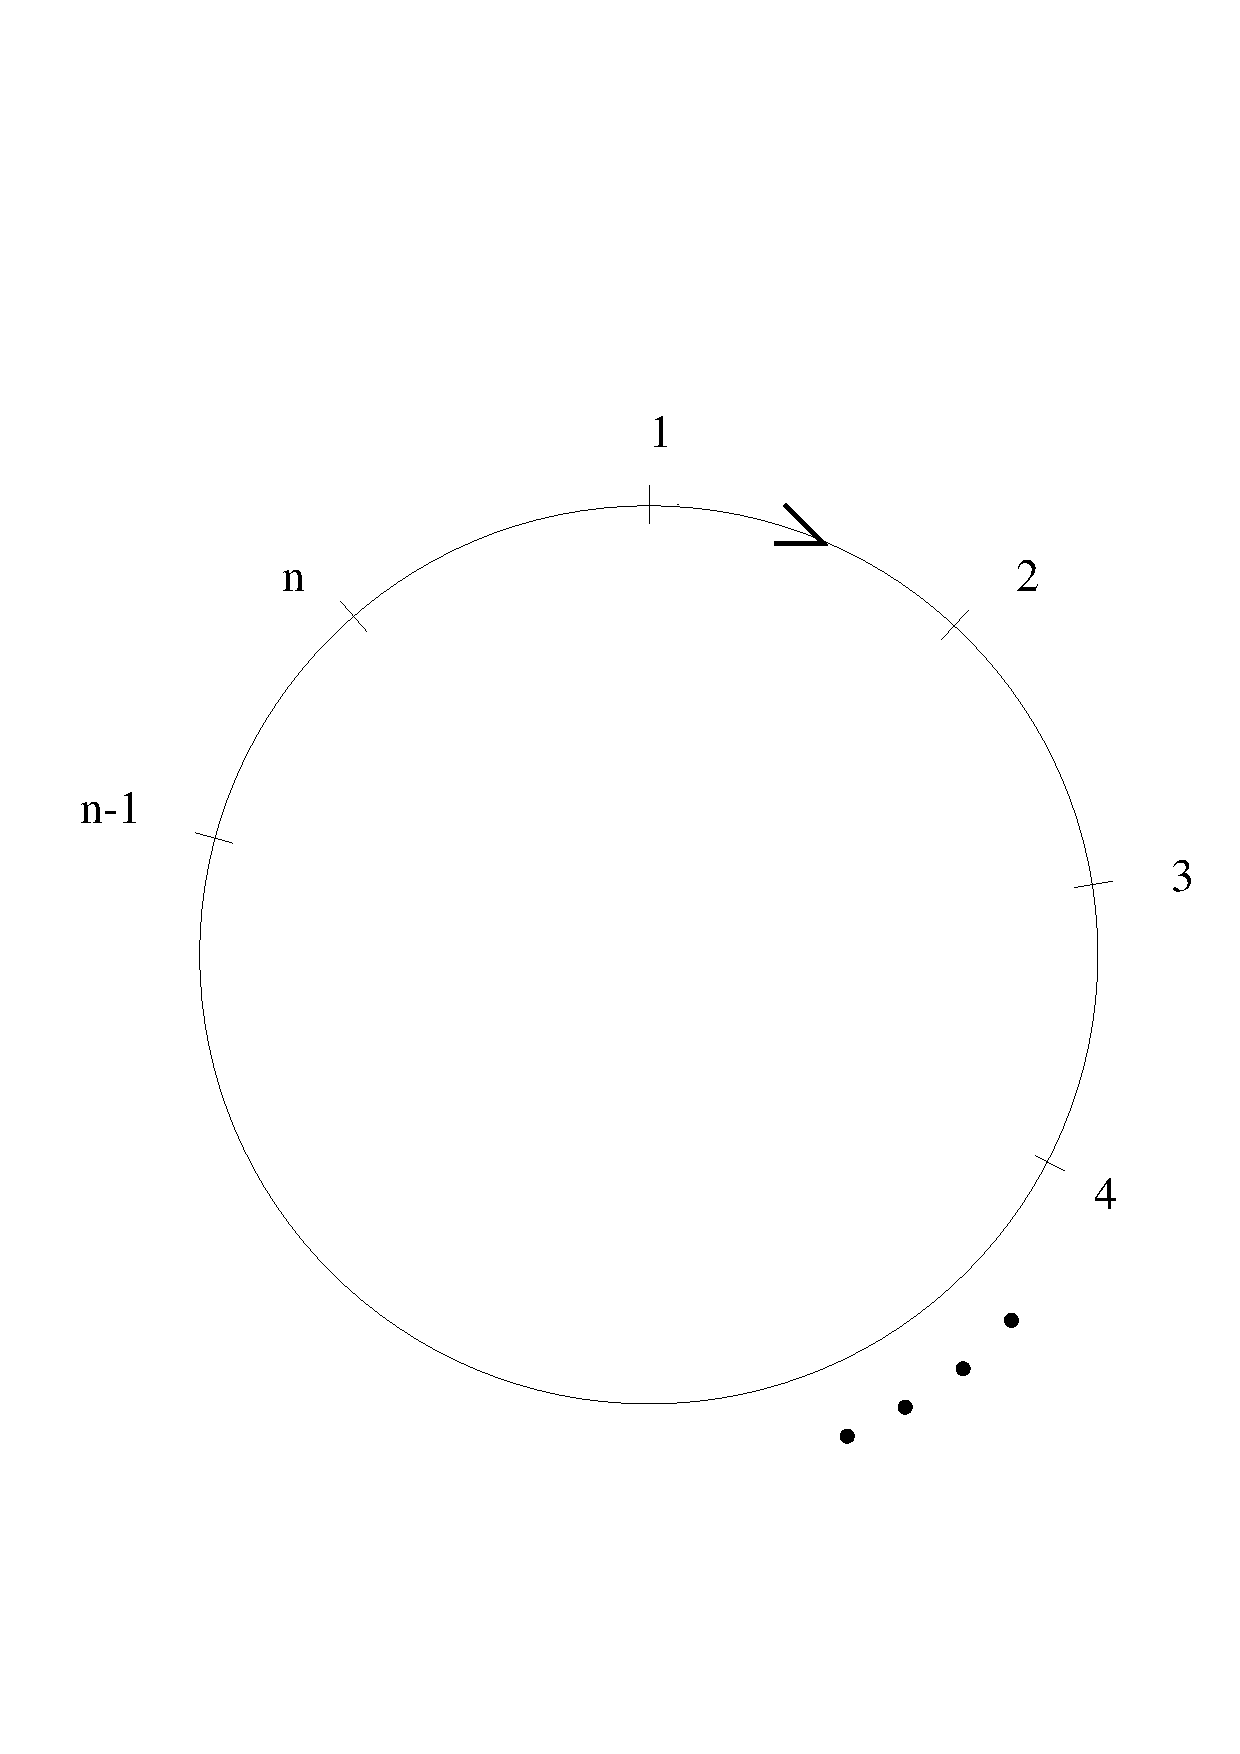
\includegraphics[height=2.5in]{fig10_10_1}
  \caption{Schematic drawing of a ring showing Poincare surfaces of
section (locations) {\em 1} through {\em n}.}
\end{figure}

Now use (2.1) and (2.4) to write ${\cal N}$ in the form
\begin{eqnarray}
{\cal N} &=& {\cal A}_1 {\cal M}_1 {\cal A}_1^{-1} = {\cal A}_1
{\cal M}_{12} {\cal M}_{23} \cdots {\cal M}_{n1} {\cal A}_1^{-1} \nonumber \\
&=& {\cal A}_1 {\cal M}_{12} {\cal A}_2^{-1} {\cal A}_2 {\cal
M}_{23} {\cal A}_3^{-1} \cdots {\cal A}_n {\cal M}_{n1} {\cal A}_1^{-1}
\nonumber \\
&=& {\cal N}_{12} {\cal N}_{23}  \cdots {\cal N}_{n1}.
\end{eqnarray}
Here the maps ${\cal N}_{12}$, ${\cal N}_{23}$, etc. are defined by the
relations
\begin{equation}
{\cal N}_{12} = {\cal A}_1 {\cal M}_{12} {\cal A}_2^{-1},
\end{equation}
\begin{equation}
{\cal N}_{23} = {\cal A}_2 {\cal M}_{23} {\cal A}_3^{-1}, \ {\rm etc.}
\end{equation}
It can be shown all the maps ${\cal N}_{12}$, ${\cal N}_{23}$, etc.
commute with each other and with ${\cal N}$, and are all in {\em normal} form.

If the ring is sufficiently subdivided, the subdivision maps ${\cal
M}_{12}$, ${\cal M}_{23}$, etc. will be near the identity.
Correspondingly the members of the map pairs ${\cal A}_i$, ${\cal
A}_{i+1}$ will be close to each other.  Consequently, the maps ${\cal
N}_{12}$, ${\cal N}_{23}$, etc. given by relations of the form (2.9) and
(2.10) will all be close to the identity.  It
follows that they can be written uniquely in the exponential form
\begin{equation}
{\cal N}_{12} = \exp (:h_{12}:),
\end{equation}
\begin{equation}
{\cal N}_{23} = \exp (:h_{23}:), \ {\rm etc.}
\end{equation}
where the Lie operators $:h_{12}:$, $:h_{23}:$, etc. are all small and
all commute.

Based on the observations above, ${\cal N}$ can be written in the form
\begin{equation}
{\cal N} = \exp (:h:)
\end{equation}
with $h$ given by the sum
\begin{equation}
h = h_{12} + h_{23} + \cdots h_{n1}.
\end{equation}
Full tunes can now be defined in terms of the coefficients of the {\em
quadratic} parts of $h$.

Exhibit 10.2.2 illustrates this procedure for the Proton Storage Ring (PSR)
using, for convenience, the subdivision introduced in section 10.9.
(Actually, this subdivision is far finer than necessary.  It is usually
sufficient to use just the maps for individual elements without
subdividing them further.  Indeed, even a coarser subdivision may be
adequate.  What is required is that the principal value of the logarithm
of each ${\cal N}_{i,i+1}$ be the correct value.)  The line {\em
benchmk} computes tunes for the {\em nsex} sector (period) map and the
one-turn {\em ring} map to be used later as comparison values.  The line
{\em setup} initializes various maps to the identity map, computes the
one-turn map and stores it as the lump {\em luring}, and computes the
corresponding ${\cal A}$ and stores it as ``script A before''.

The stage is now set for \Mary to step its way around the ring using the
line {\em \%ring}.  At each location marked by a \%, {\em work} is invoked
to carry out the following tasks:
\begin{quote}
Compute the Poincare surface of section map ${\cal M}_i$ for that
location. \\

Compute and store ${\cal A}_i$ (script A after) and ${\cal A}^{-1}_i$ for
that location. \\

Compute ${\cal N}_{i-1,i} = {\cal A}_{i-1} {\cal M}_{i-1,i} {\cal
A}_i^{-1}$, the transformed current map. \\

Compute the ``phase advances'' (scaled exponents) for ${\cal N}_{i-1,i}$
with the aid of the {\em lnf} command (see section 8.41), and add these
phase advances to the running total.  \\

Update ${\cal A}$.
\end{quote}

Finally, the line {\em tunes} accesses and displays the final {\em total}
tunes.  Observe that $f(7)$ is 10 times the horizontal tune for the
sector {\em nsex}, and $f(18)$ is 10 times the vertical tune for the
sector {\em nsex}.  This is as it should be, because the full PSR is made
of 10 identical sectors (apart from sextupoles whose contribution to
tunes is the same as the drift spaces they replace).  Note also that the
fractional horizontal and vertical tunes computed from the one-turn map
{\em ring} agree with the fractional parts of $f(9)$ and $f(18)$,
respectively.

\begin{footnotesize}
\begin{verbatim}
Exhibit 10.2.2
***MARYLIE 3.0***
Prerelease Development Version 8/21/98
Copyright 1987 Alex J. Dragt
All rights reserved

Data input complete; going into #labor.
#comment
 Exhibit 10.2.2.
       This is a MaryLie run that illustrates the computation of full tunes
  (including integer parts) using the PSR as an example.  To compute full tunes
  of a circulating lattice, it is necessary to subdivide the lattice into
  sufficiently small pieces.  In this case the dipoles and the long and
  medium-long drifts are split into 5 pieces.  Quads and sextupoles are
  split in two.  This splitting is the same as that used in exhibit 10.9.
  For the purposes of this example such a fine subdivision of the lattice
  is in fact unnecessary.  It would have been sufficient to have simply used
  the maps for the individual beam-line elements.

  The following acronyms are used:
  scurmap = store current map
  gcurmap = get current map
  scummap = store cumulative map
  gcummap = get cumulative map
  sab = store script A before
  gab = get script A before
  saa = store script A after
  gaa = get script A after
  saai = store script A after inverse
  gaai = get script A after inverse
  spha = store phase advance
  gpha = get phase advance
  benchmk = bench mark
  cpssmap = compute Poincare surface of section map
  caa&aai = compute script A afterward and script A afterward inverse
  tcurmap = transform current map
  adpha = add phase advance

 #beam
   4.86914813175970
  0.849425847892200
   1.00000000000000
   1.00000000000000
 #menu
  drvs     drft
   0.300000000000000
  drs      drft
   0.450000000000000
  cdrml    drft
    1.48646000000000
  drml/5   drft
   0.297292000000000
  cdrl     drft
    2.28646000000000
  drl/5    drft
   0.457292000000000
  cbend    pbnd
    36.0000000000000      0.000000000000000E+00  0.500000000000000
    1.20000000000000
  inprot   prot
    18.0000000000000       1.00000000000000
  outprot  prot
    18.0000000000000       2.00000000000000
  infrng   frng
    18.0000000000000      0.000000000000000E+00  0.000000000000000E+00
    1.20000000000000       1.00000000000000
  outfrng  frng
    18.0000000000000      0.000000000000000E+00  0.000000000000000E+00
    1.20000000000000       2.00000000000000
  ingbdy   gbdy
   0.000000000000000E+00   18.0000000000000      0.000000000000000E+00
    1.20000000000000
  outgbdy  gbdy
   0.000000000000000E+00  0.000000000000000E+00   18.0000000000000
    1.20000000000000
  sbend/5  nbnd
    7.20000000000000      0.000000000000000E+00  0.500000000000000
    1.20000000000000      0.000000000000000E+00  0.000000000000000E+00
  chfq     quad
   0.500000000000000       2.72000000000000       1.00000000000000
    1.00000000000000
  inhfq    quad
   0.250000000000000       2.72000000000000       1.00000000000000
   0.000000000000000E+00
  outhfq   quad
   0.250000000000000       2.72000000000000      0.000000000000000E+00
    1.00000000000000
  chdq     quad
   0.500000000000000      -1.92000000000000       1.00000000000000
    1.00000000000000
  inhdq    quad
   0.250000000000000      -1.92000000000000       1.00000000000000
   0.000000000000000E+00
  outhdq   quad
   0.250000000000000      -1.92000000000000      0.000000000000000E+00
    1.00000000000000
  chcs     sext
   0.500000000000000      0.000000000000000E+00
  hcs/2    sext
   0.250000000000000      0.000000000000000E+00
  cvcs     sext
   0.500000000000000      0.000000000000000E+00
  vcs/2    sext
   0.250000000000000      0.000000000000000E+00
  fileout  pmif
    1.00000000000000       12.0000000000000       3.00000000000000
  snor     snor
   0.000000000000000E+00   2.00000000000000      0.000000000000000E+00
   0.000000000000000E+00  0.000000000000000E+00
  tasm     tasm
    1.00000000000000      1.000000000000000E-03   1.00000000000000
   0.000000000000000E+00   3.00000000000000      0.000000000000000E+00
  iden     iden
  inv      inv
  scurmap  stm
    1.00000000000000
  gcurmap  gtm
    1.00000000000000       1.00000000000000
  scummap  stm
    2.00000000000000
  gcummap  gtm
    1.00000000000000       2.00000000000000
  sab      stm
    3.00000000000000
  gab      gtm
    1.00000000000000       3.00000000000000
  saa      stm
    4.00000000000000
  gaa      gtm
    1.00000000000000       4.00000000000000
  saai     stm
    5.00000000000000
  gaai     gtm
    1.00000000000000       5.00000000000000
  spha     stm
    6.00000000000000
  gpha     gtm
    2.00000000000000       6.00000000000000
  gbuf1    gbuf
    2.00000000000000       1.00000000000000
  padd     padd
   0.000000000000000E+00   6.00000000000000       6.00000000000000
  wcl10    wcl
    3.00000000000000       10.0000000000000       3.00000000000000
  setzero  zer
   0.000000000000000E+00  1.000000000000000E-07  0.000000000000000E+00
  mapout   ptm
    3.00000000000000       3.00000000000000      0.000000000000000E+00
   0.000000000000000E+00   1.00000000000000
  matout   ptm
    3.00000000000000      0.000000000000000E+00  0.000000000000000E+00
   0.000000000000000E+00   1.00000000000000
  fout     ptm
   0.000000000000000E+00   3.00000000000000      0.000000000000000E+00
   0.000000000000000E+00   1.00000000000000
  lnf      lnf
    1.00000000000000       1.00000000000000       2.00000000000000
  fin      end
 #lines
  drml
      5*drml/5
  drl
      5*drl/5
  bend
      1*inprot      1*infrng      1*ingbdy      5*sbend/5     1*outgbdy  &
      1*outfrng     1*outprot
  hfq
      1*inhfq       1*outhfq
  hdq
      1*inhdq       1*outhdq
  hcs
      2*hcs/2
  vcs
      2*vcs/2
  nsex
      1*drl         1*hdq         1*drs         1*bend        1*drs      &
      1*hfq         1*drl
  tsex
      1*drl         1*hdq         1*drs         1*bend        1*drs      &
      1*hfq         1*drvs        1*hcs         1*drml
  lsex
      1*drml        1*vcs         1*drvs        1*hdq         1*drs      &
      1*bend        1*drs         1*hfq         1*drl
  half
      1*nsex        1*tsex        1*lsex        1*nsex        1*nsex
  ring
      2*half
  %ring
      1*%           1*drl/5       1*%           1*drl/5       1*%        &
      1*drl/5       1*%           1*drl/5       1*%           1*drl/5    &
      1*%           1*inhdq       1*%           1*outhdq      1*%        &
      1*drs         1*%           1*inprot      1*%           1*infrng   &
      1*%           1*ingbdy      1*%           1*sbend/5     1*%        &
      1*sbend/5     1*%           1*sbend/5     1*%           1*sbend/5  &
      1*%           1*sbend/5     1*%           1*outgbdy     1*%        &
      1*outfrng     1*%           1*outprot     1*%           1*drs      &
      1*%           1*inhfq       1*%           1*outhfq      1*%        &
      1*drl/5       1*%           1*drl/5       1*%           1*drl/5    &
      1*%           1*drl/5       1*%           1*drl/5       1*%        &
      1*drl/5       1*%           1*drl/5       1*%           1*drl/5    &
      1*%           1*drl/5       1*%           1*drl/5       1*%        &
      1*inhdq       1*%           1*outhdq      1*%           1*drs      &
      1*%           1*inprot      1*%           1*infrng      1*%        &
      1*ingbdy      1*%           1*sbend/5     1*%           1*sbend/5  &
      1*%           1*sbend/5     1*%           1*sbend/5     1*%        &
      1*sbend/5     1*%           1*outgbdy     1*%           1*outfrng  &
      1*%           1*outprot     1*%           1*drs         1*%        &
      1*inhfq       1*%           1*outhfq      1*%           1*drvs     &
      1*%           1*hcs/2       1*%           1*hcs/2       1*%        &
      1*drml/5      1*%           1*drml/5      1*%           1*drml/5   &
      1*%           1*drml/5      1*%           1*drml/5      1*%        &
      1*drml/5      1*%           1*drml/5      1*%           1*drml/5   &
      1*%           1*drml/5      1*%           1*drml/5      1*%        &
      1*vcs/2       1*%           1*vcs/2       1*%           1*drvs     &
      1*%           1*inhdq       1*%           1*outhdq      1*%        &
      1*drs         1*%           1*inprot      1*%           1*infrng   &
      1*%           1*ingbdy      1*%           1*sbend/5     1*%        &
      1*sbend/5     1*%           1*sbend/5     1*%           1*sbend/5  &
      1*%           1*sbend/5     1*%           1*outgbdy     1*%        &
      1*outfrng     1*%           1*outprot     1*%           1*drs      &
      1*%           1*inhfq       1*%           1*outhfq      1*%        &
      1*drl/5       1*%           1*drl/5       1*%           1*drl/5    &
      1*%           1*drl/5       1*%           1*drl/5       1*%        &
      1*drl/5       1*%           1*drl/5       1*%           1*drl/5    &
      1*%           1*drl/5       1*%           1*drl/5       1*%        &
      1*inhdq       1*%           1*outhdq      1*%           1*drs      &
      1*%           1*inprot      1*%           1*infrng      1*%        &
      1*ingbdy      1*%           1*sbend/5     1*%           1*sbend/5  &
      1*%           1*sbend/5     1*%           1*sbend/5     1*%        &
      1*sbend/5     1*%           1*outgbdy     1*%           1*outfrng  &
      1*%           1*outprot     1*%           1*drs         1*%        &
      1*inhfq       1*%           1*outhfq      1*%           1*drl/5    &
      1*%           1*drl/5       1*%           1*drl/5       1*%        &
      1*drl/5       1*%           1*drl/5       1*%           1*drl/5    &
      1*%           1*drl/5       1*%           1*drl/5       1*%        &
      1*drl/5       1*%           1*drl/5       1*%           1*inhdq    &
      1*%           1*outhdq      1*%           1*drs         1*%        &
      1*inprot      1*%           1*infrng      1*%           1*ingbdy   &
      1*%           1*sbend/5     1*%           1*sbend/5     1*%        &
      1*sbend/5     1*%           1*sbend/5     1*%           1*sbend/5  &
      1*%           1*outgbdy     1*%           1*outfrng     1*%        &
      1*outprot     1*%           1*drs         1*%           1*inhfq    &
      1*%           1*outhfq      1*%           1*drl/5       1*%        &
      1*drl/5       1*%           1*drl/5       1*%           1*drl/5    &
      1*%           1*drl/5       1*%           1*drl/5       1*%        &
      1*drl/5       1*%           1*drl/5       1*%           1*drl/5    &
      1*%           1*drl/5       1*%           1*inhdq       1*%        &
      1*outhdq      1*%           1*drs         1*%           1*inprot   &
      1*%           1*infrng      1*%           1*ingbdy      1*%        &
      1*sbend/5     1*%           1*sbend/5     1*%           1*sbend/5  &
      1*%           1*sbend/5     1*%           1*sbend/5     1*%        &
      1*outgbdy     1*%           1*outfrng     1*%           1*outprot  &
      1*%           1*drs         1*%           1*inhfq       1*%        &
      1*outhfq      1*%           1*drl/5       1*%           1*drl/5    &
      1*%           1*drl/5       1*%           1*drl/5       1*%        &
      1*drl/5       1*%           1*drl/5       1*%           1*drl/5    &
      1*%           1*drl/5       1*%           1*drl/5       1*%        &
      1*drl/5       1*%           1*inhdq       1*%           1*outhdq   &
      1*%           1*drs         1*%           1*inprot      1*%        &
      1*infrng      1*%           1*ingbdy      1*%           1*sbend/5  &
      1*%           1*sbend/5     1*%           1*sbend/5     1*%        &
      1*sbend/5     1*%           1*sbend/5     1*%           1*outgbdy  &
      1*%           1*outfrng     1*%           1*outprot     1*%        &
      1*drs         1*%           1*inhfq       1*%           1*outhfq   &
      1*%           1*drvs        1*%           1*hcs/2       1*%        &
      1*hcs/2       1*%           1*drml/5      1*%           1*drml/5   &
      1*%           1*drml/5      1*%           1*drml/5      1*%        &
      1*drml/5      1*%           1*drml/5      1*%           1*drml/5   &
      1*%           1*drml/5      1*%           1*drml/5      1*%        &
      1*drml/5      1*%           1*vcs/2       1*%           1*vcs/2    &
      1*%           1*drvs        1*%           1*inhdq       1*%        &
      1*outhdq      1*%           1*drs         1*%           1*inprot   &
      1*%           1*infrng      1*%           1*ingbdy      1*%        &
      1*sbend/5     1*%           1*sbend/5     1*%           1*sbend/5  &
      1*%           1*sbend/5     1*%           1*sbend/5     1*%        &
      1*outgbdy     1*%           1*outfrng     1*%           1*outprot  &
      1*%           1*drs         1*%           1*inhfq       1*%        &
      1*outhfq      1*%           1*drl/5       1*%           1*drl/5    &
      1*%           1*drl/5       1*%           1*drl/5       1*%        &
      1*drl/5       1*%           1*drl/5       1*%           1*drl/5    &
      1*%           1*drl/5       1*%           1*drl/5       1*%        &
      1*drl/5       1*%           1*inhdq       1*%           1*outhdq   &
      1*%           1*drs         1*%           1*inprot      1*%        &
      1*infrng      1*%           1*ingbdy      1*%           1*sbend/5  &
      1*%           1*sbend/5     1*%           1*sbend/5     1*%        &
      1*sbend/5     1*%           1*sbend/5     1*%           1*outgbdy  &
      1*%           1*outfrng     1*%           1*outprot     1*%        &
      1*drs         1*%           1*inhfq       1*%           1*outhfq   &
      1*%           1*drl/5       1*%           1*drl/5       1*%        &
      1*drl/5       1*%           1*drl/5       1*%           1*drl/5    &
      1*%           1*drl/5       1*%           1*drl/5       1*%        &
      1*drl/5       1*%           1*drl/5       1*%           1*drl/5    &
      1*%           1*inhdq       1*%           1*outhdq      1*%        &
      1*drs         1*%           1*inprot      1*%           1*infrng   &
      1*%           1*ingbdy      1*%           1*sbend/5     1*%        &
      1*sbend/5     1*%           1*sbend/5     1*%           1*sbend/5  &
      1*%           1*sbend/5     1*%           1*outgbdy     1*%        &
      1*outfrng     1*%           1*outprot     1*%           1*drs      &
      1*%           1*inhfq       1*%           1*outhfq      1*%        &
      1*drl/5       1*%           1*drl/5       1*%           1*drl/5    &
      1*%           1*drl/5       1*%           1*drl/5       1*%
  benchmk
      1*nsex        1*tasm        1*iden        1*ring        1*tasm     &
      1*iden
  setup
      1*setzero     1*iden        1*scurmap     1*scummap     1*spha     &
      1*luring      1*snor        1*gbuf1       1*sab         1*iden
  %
      1*work
  work
      1*scurmap     1*cpssmap     1*caa&aai     1*tcurmap     1*adpha    &
      1*update      1*iden
  cpssmap
      1*iden        1*gcummap     1*gcurmap     1*scummap     1*inv      &
      1*luring      1*gcummap
  caa&aai
      1*snor        1*gbuf1       1*saa         1*inv         1*saai
  tcurmap
      1*iden        1*gab         1*gcurmap     1*gaai
  adpha
      1*lnf         1*gbuf1       1*padd
  update
      1*iden        1*gaa         1*sab
  tunes
      1*gpha        1*fout
 #lumps
  luring
      1*ring
 #loops
  lring
      1*ring
 #labor
     1*fileout
     1*benchmk
     1*setup
     1*%ring
     1*tunes
     1*fin

*********************************************
* Calculation of tunes for the nsex sector: *
*********************************************

 twiss analysis of static map

 tunes and chromaticities for delta defined in terms of P sub tau:

 horizontal tune =  0.225410281174760
 first order horizontal chromaticity =  0.110337520026812
 second order horizontal chromaticity =   3.75197479724374
 horizontal tune when delta =  1.000000000000000E-003
  0.225524370669584

 vertical tune =  0.225543770585176
 first order vertical chromaticity =  0.250986502239161
 second order vertical chromaticity =   2.18869156252695
 vertical tune when delta =  1.000000000000000E-003
  0.225796945778978

 tune separation when delta=  1.000000000000000E-003
 -2.725751093941298E-004

 normalized anharmonicities
  hhn=  0.481212294862244
  vvn=  0.287510196121498
  hvn=  0.489194351436008

*******************************************
* Calculation of (fractional) tunes using *
* the one-turn map for the whole ring:    *
*******************************************

 twiss analysis of static map

 tunes and chromaticities for delta defined in terms of P sub tau:

 horizontal tune =  0.254102811747597
 first order horizontal chromaticity =   1.10337520026812
 second order horizontal chromaticity =   37.5197479724370
 horizontal tune when delta =  1.000000000000000E-003
  0.255243706695837

 vertical tune =  0.255437705851762
 first order vertical chromaticity =   2.50986502239162
 second order vertical chromaticity =   21.8869156252694
 vertical tune when delta =  1.000000000000000E-003
  0.257969457789779

 tune separation when delta=  1.000000000000000E-003
 -2.725751093941298E-003

 normalized anharmonicities
  hhn=   4.81212294862237
  vvn=   2.87510196121501
  hvn=   4.89194351436007

lump luring   constructed and stored.( 1)

****************
* Total tunes: *
****************

nonzero elements in generating polynomial are :

 f(  7)=f( 20 00 00 )=  2.2541028117476
 f( 13)=f( 02 00 00 )=  2.2541028117476
 f( 18)=f( 00 20 00 )=  2.2554377058518
 f( 22)=f( 00 02 00 )=  2.2554377058518

end of MARYLIE run
\end{verbatim}
\end{footnotesize}

\subsection{Computation of Tune Foot Print}\label{footprint} \index{tune foot print} \index{foot print}
Exhibit 8.2 in section 8.2 illustrated the use of a {\em tasm} command to compute the tunes for a single particle in a static ring.  It is also possible to compute all the tunes for a collection of particles.  This can be done by preparing a particle distribution and repeatedly using a tasm command within a logical loop.  The particle distribution is stored on an external file, and particle phase-space coordinates are read in particle-by-particle from this file with the aid of a random parameter set command. A {\em tasm} command then takes these coordinates from the parameter set and computes the tunes for each particle.   Finally, the tunes for each particle can be written on an external file (with the aid of {\em sq} and {\em wsq} commands) for subsequent plotting to produce a tune footprint for the particle distribution.  (See section 7.26 for a description of the use of random parameter sets.)  Exhibits 10.2.3a and 10.2.3b below illustrate this process for a simple example.  Exhibit 10.2.3a displays the instructions for the {\em sq} command that along with the {\em wsq} command are used to write out the array entries tn(1,3) and tn(2,3).  (See sections 8.26 and 9.5).  Exhibit 10.2.3b shows the \Mary run itself.  Note that in this example a simple set of preliminary commands was used to generate a particle distribution.  However, this distribution could have come from anywhere.

Figures 10.2.3.1 through 10.2.3.3 display the particle distribution.  Figure 10.2.3.4 shows the footprint in tune space produced by this distribution for the case of the PSR.  Finally, note that a similar process could have been carried out for a dynamic ring by using a {\em tadm} command.  In this case, the tune footprint would be three dimensional.


\vspace{.25in}
\noindent Exhibit 10.2.3 a: Contents of file 15 that provides instructions for the {\em sq} command.
\begin{footnotesize}
\begin{verbatim}
1 tn(1,3)
2 tn(2,3)
#
\end{verbatim}
\end{footnotesize}

\vspace{.25in}
\noindent Exhibit 10.2.3b: \Mary run illustrating the computation of tunes for a distribution of particles.
\begin{footnotesize}
\begin{verbatim}
#comment
  Exhibit 10.2.3
  This MaryLie run illustrates the computation of a tune footprint.
  For simplicity, a tune footprint is computed for the PSR ring
  of Section 2.5. This run consists of three parts:

   a) Generation of the 1-turn map.

   b) Generation of a particle distribution.  This is done by the line
      makeic.  For convenience, a gaussian distribution is used. The
      particle distribution is written on file 14.

   c) Computation of the tune footprint for this distribution.  This
      is done using a logical loop.  Rays are read in one at a time
      from file 14 using the random parameter set command rptdata.
      Instructions for sq, which is invoked before entering the loop,
      are taken from file 15.  Tunes are written on file 16 for
      subsequent plotting.

#beam
   4.86914813175970
  0.849425847892200
   1.00000000000000
   1.00000000000000
#menu
  drvs     drft
   0.300000000000000
  drs      drft
   0.450000000000000
  drml     drft
    1.48646000000000
  drl      drft
    2.28646000000000
  bend     pbnd
    36.0000000000000      0.000000000000000E+00  0.500000000000000
    1.20000000000000
  hfq      quad
   0.500000000000000       2.72000000000000       1.00000000000000
    1.00000000000000
  hdq      quad
   0.500000000000000      -1.92000000000000       1.00000000000000
    1.00000000000000
  hcs      sext
   0.500000000000000      0.000000000000000E+00
  vcs      sext
   0.500000000000000      0.000000000000000E+00
  fileout  pmif
    1.00000000000000       12.0000000000000       3.00000000000000
  mapout   ptm
    3.00000000000000       3.00000000000000      0.000000000000000E+00
   0.000000000000000E+00   1.00000000000000
  tasmpt   tasm
    1.00000000000000       1.00000000000000       1.00000000000000
   0.000000000000000E+00   3.00000000000000      0.000000000000000E+00
  qtasmpt  tasm
    1.00000000000000       1.00000000000000       1.00000000000000
   0.000000000000000E+00  0.000000000000000E+00  0.000000000000000E+00
  ptdata   ps1
   1.000000000000000E-02  0.000000000000000E+00  1.000000000000000E-02
   0.000000000000000E+00  0.000000000000000E+00  1.000000000000000E-03
  rptdata  rps1
    14.0000000000000      0.000000000000000E+00
  clear    iden
  zer      zer
   0.000000000000000E+00  1.000000000000000E-10  1.000000000000000E-10
   0.000000000000000E+00
  fin      end
  sho3     shoa
    3.00000000000000       1.00000000000000      0.000000000000000E+00
  bip      bip
    100.000000000000
  tip      tip
   0.000000000000000E+00
  sq       sq
    15.0000000000000      0.000000000000000E+00   1.00000000000000
    1.00000000000000
  wsq      wsq
    1.00000000000000       1.00000000000000       16.0000000000000
    1.00000000000000       1.00000000000000      0.000000000000000E+00
  bgendat  ps1
   1.000000000000000E-04  1.000000000000000E-04  1.000000000000000E-04
    5.00000000000000      0.000000000000000E+00  0.000000000000000E+00
  bgen     bgen
    6.00000000000000       123.000000000000       100.000000000000
    137.000000000000       1.00000000000000       1.00000000000000
  raysout  rt
   0.000000000000000E+00   14.0000000000000      0.000000000000000E+00
   0.000000000000000E+00   1.00000000000000      0.000000000000000E+00
#lines
  nsex
      1*drl         1*hdq         1*drs         1*bend        1*drs      &
      1*hfq         1*drl
  tsex
      1*drl         1*hdq         1*drs         1*bend        1*drs      &
      1*hfq         1*drvs        1*hcs         1*drml
  lsex
      1*drml        1*vcs         1*drvs        1*hdq         1*drs      &
      1*bend        1*drs         1*hfq         1*drl
  half
      1*nsex        1*tsex        1*lsex        1*nsex        1*nsex
  ring
      2*half
  makeic
      1*bgendat     1*bgen        1*raysout
#lumps
#loops
#labor
     1*fileout
     1*ring
     1*makeic
     1*sq
     1*bip
     1*rptdata
     1*qtasmpt
     1*wsq
     1*tip
     1*fin

         100 rays generated

  numerically computed values of selected moments
  values of <x*x>, <x*px>, <px*px>:
  9.425467645700800E-005 -1.354881408024196E-005  1.017819260324027E-004
  values of <y*y>, <y*py>, <py*py>:
  1.082160291148366E-004  6.573236882795287E-006  8.852331615780860E-005
  values of <t*t>, <t*pt>, <pt*pt>:
  1.134396798850281E-004  2.404587894362543E-005  9.217736080450674E-005

  analytically computed values of selected moments
  values of <x*x>, <x*px>, <px*px>:
  1.000000000000000E-004  0.000000000000000E+000  1.000000000000000E-004
  values of <y*y>, <y*py>, <py*py>:
  1.000000000000000E-004  0.000000000000000E+000  1.000000000000000E-004
  values of <t*t>, <t*pt>, <pt*pt>:
  1.000000000000000E-004  0.000000000000000E+000  1.000000000000000E-004

  In subroutine sq
accept  1:     tn(1,3)
accept  2:     tn(2,3)

  Aims/quantities selected :
No.     item      present value
----------------------------------
  1   tn(1,3) =      0.000000000E+00
  2   tn(2,3) =      0.000000000E+00

end of MARYLIE run
\end{verbatim}
\end{footnotesize}


\newpage
\renewcommand{\thefigure}{\arabic{chapter}.\arabic{section}.\arabic{subsection}.\arabic{figure}}
\setcounter{figure}{0}
\begin{figure}[h]
  \centering
  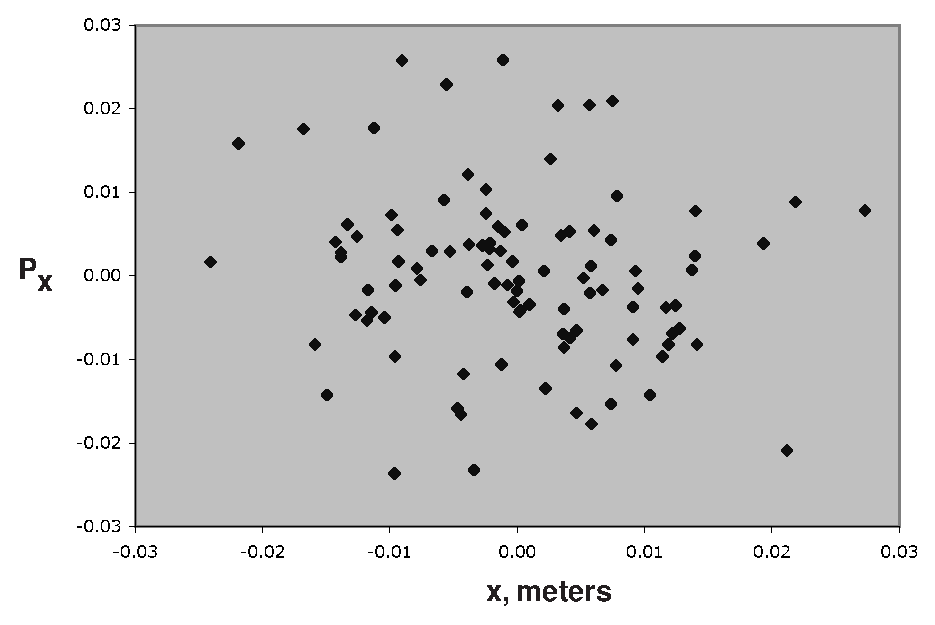
\includegraphics[height=2.7in]{fig10_2_3_1}
  \caption{Horizontal projection of phase-space distribution produced by plotting the first two columns of file 14.}
\end{figure}


\begin{figure}[h]
  \centering
  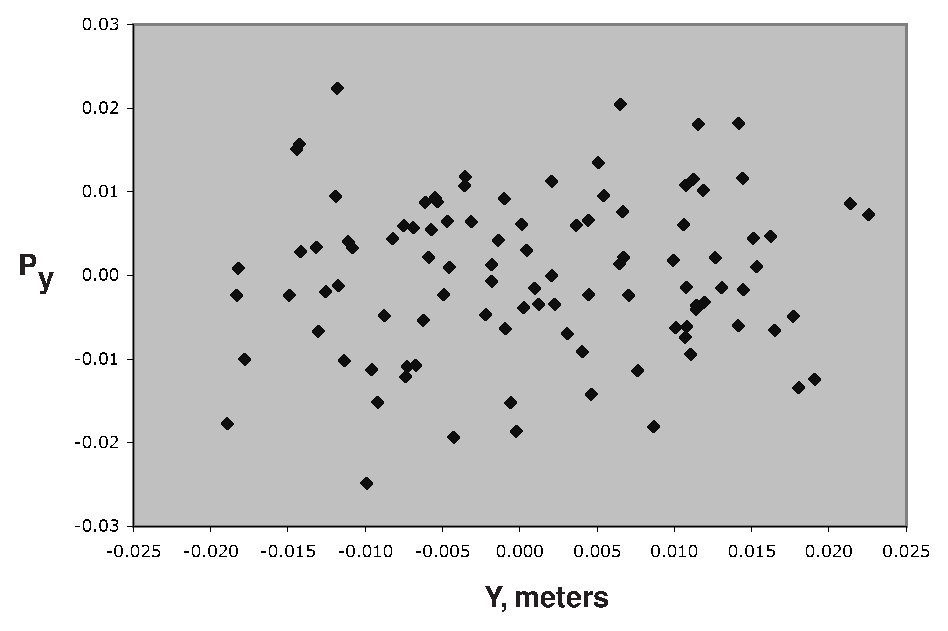
\includegraphics[height=2.7in]{fig10_2_3_2}
  \caption{Vertical projection of phase-space distribution produced by plotting the third and fourth columns of file 14.}
\end{figure}

\newpage
\begin{figure}[h]
  \centering
  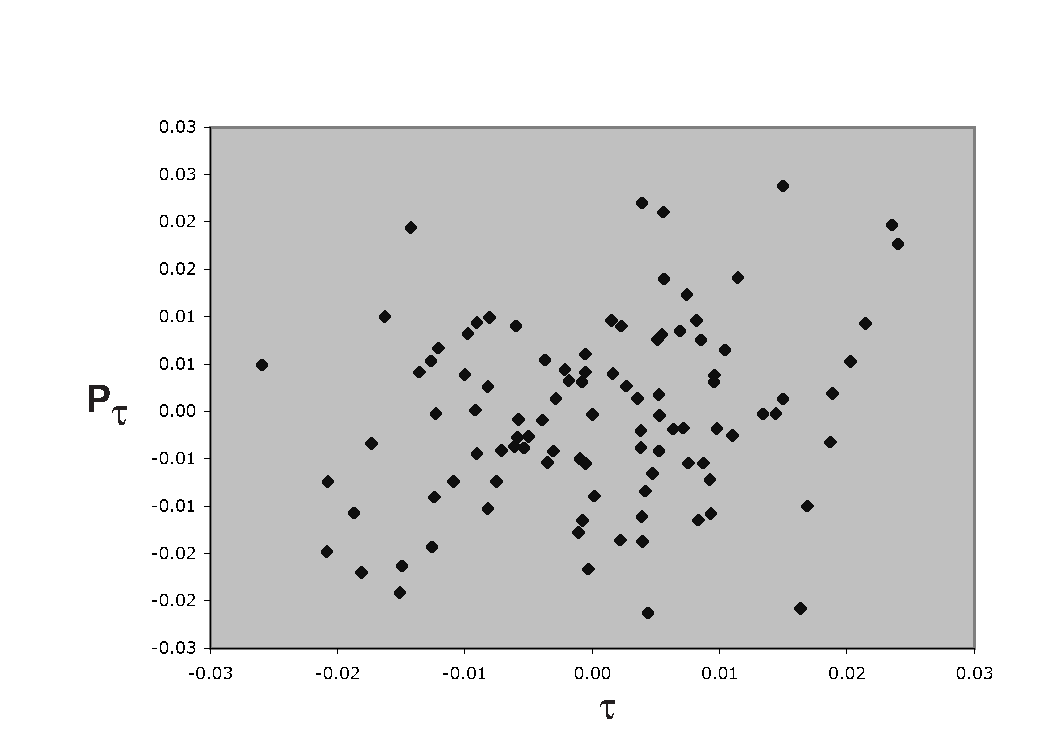
\includegraphics[height=2.7in]{fig10_2_3_3}
  \caption{Temporal projection of phase-space distribution produced by plotting the last two columns of file 14.}
\end{figure}

\begin{figure}[h]
  \centering
  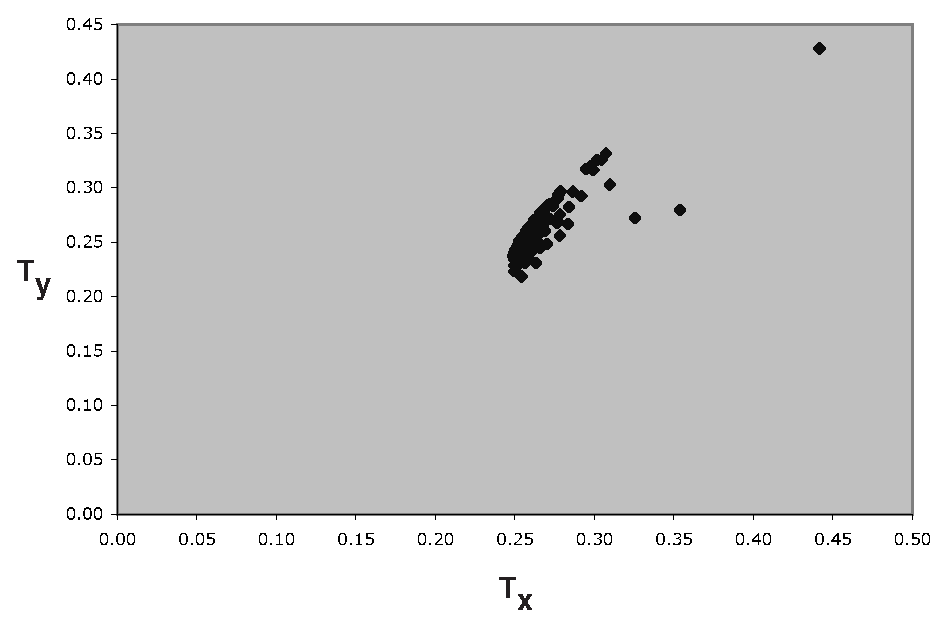
\includegraphics[height=2.7in]{fig10_2_3_4}
  \caption{Tune footprint associated with the distribution shown in Figures 10.2.3.1 through 10.2.3.3 and produced by plotting the contents of file 16.}
\end{figure}


\newpage
\section[Octupole Correction \& Optimization of a Quadrupole $\cdots$]{Octupole Correction and Optimization of a Quadrupole Spot Forming System}
\label{octcorrect}
Section 2.2 illustrated the importance of certain third-order aberrations
for governing the performance of a spot forming system.  See figure
2.2.2.  In the examples of this section these aberrations are corrected with
the aid of octupoles.  In subsection 10.3.1 the simple quadrupoles in
the triplet of figure 2.2.1 are replaced with combined-function quadrupoles
that are capable of having an octupole component.  See section 6.24.  The
octupole components of these combined-function quadrupoles are then
varied to correct the detrimental third-order aberrations.  In subsection
10.3.2 four additional octupoles are added to the system and all seven
octupole strengths are then varied to find an optimized fit.  Finally,
in subsection 10.3.3, the same optimized fitting is carried out using the
{\em mss} optimizer.\index{spherical aberration} \index{aberrations} \index{corrector} \index{microprobe}

%\numberbysubsection
\subsection{Fitting Three Quadrupole and Three Octupole Strengths}
\label{three} \index{octupole correction} \index{spot forming system} \index{fit}
The first part of the \Mary run for this example, shown in Exhibit 10.3.1, is devoted to fitting the
quadrupole strengths in order to achieve the paraxial spot-forming
condition $r(1,1) = r(3,3) = 0$.  In this case there are three
quadrupole strengths to be adjusted with the constraint that the outer
quadrupoles should have the same strengths.  This is accomplished by
taking three steps:
\begin{enumerate}
\renewcommand{\theenumi}{roman{enumi}}
\item At the beginning of the \Mary run the inner and outer quads are
given the same nominal strengths (.1 Tesla/meter).
\item The ``vary'' command {\em qvary} that is used to vary the
quadrupoles has the value JOB=$-$1 for its first parameter.  See section 9.6.
\item The variation of the third quadrupole strength, parm3(1), is
required to be the same as that of the first quadrupole strength.  See
the italicized text entry ``{\em 1 1}'' in the quadrupole fitting part of
the Exhibit.
\end{enumerate}

The second part of the run is devoted to adjusting the three normal
octupole components of the three combined function quadrupoles to achieve
the goal $f(140) = f(149) = f(195) = 0$ for the Lie generators of the net
transfer map for the full system.  (It can be shown that these are the
Lie generators for the offensive geometric aberrations of a spot-forming
system.)  In this case there are no constraints and the ``vary" command
{\em ovary} is used with JOB=1 to vary the strength of the octupole
components.

In the third part of the run rays are traced through the
octupole-corrected spot-forming system using the net transfer map for the
full system.  The results of this ray trace are shown in figure 10.3.1.1,
which is to be compared with figure 2.2.3.  Evidently, within the achieved
numerical accuracy of the paraxial fitting requirement $r(1,1) = r(3,3) =
0$, all the rays of figure 2.2.2 are now brought to a point.  This is
because the ray trace has been done through third order using a single
map, and all the detrimental geometric third-order aberrations for a
spot-forming system have been fit to zero.

Of course, there are also detrimental higher-order aberrations beyond
third order.  An estimate of the effect of these aberrations can be had
by tracing rays element-by-element rather than using a single map.  In
this way, although the map for each element is still used only through
third order, at least the higher-order aberrations associated with
concatenating these elements can be estimated. \index{element by element}

As illustrated in the fourth part of the run, element-by-element ray
tracing can be achieved by invoking the loop {\em onebyone} whose
content is {\em cspot}, and use of the ``circ'' command {\em circ15}.
The result of this element-by-element ray trace is shown in figure 10.3.1.2,
which should also be compared with figure 2.2.3.  Now, thanks to octupole
correction, the spot size has shrunk from its initial value of $4 \times
10^{-7}$ meters (see figure 2.2.3) to an estimated value of $1 \times
10^{-8}$ meters (see figure 10.3.1.2).

\begin{footnotesize}
\begin{verbatim}
***MARYLIE 3.0***
Prerelease Development Version 5/25/98
Copyright 1987 Alex J. Dragt
All rights reserved

Data input complete; going into #labor.
#comment
 Exhibit 10.3.1.
 This is a MARYLIE run that demonstrates the use of three octupoles to
 correct three offensive aberrations in the simple spot forming system
 of Section 2.2.  To do this the simple quadrupoles are replaced with
 combined function quadrupoles having a possible octupole component.
 This run does four things:

  a) It adjusts quad strengths as an example of fitting of matrix
     elements and the use of simple constraints.

  b) It adjusts three octupole strengths to remove ("zero out") three
     Lie generators corresponding to three third-order geometrical
     aberrations that are detrimental to the performance of a
     spot forming system.  These Lie generators are:

     f(140)=f( 04 00 00 ),
     f(149)=f( 02 02 00 ), and
     f(195)=f( 00 04 00 ).

  c) It traces rays through this corrected system using the total
     transfer map.

  d) To give a rough indication of residual fifth-order aberration
     effects, rays are also traced element-by-element through the
     corrected system.  Doing so illustrates as well use of the
     element-by-element tracking ("turtle") feature of MaryLie
     acomplished with the aid of a loop and a 'circ' command.

 The beam parameters are those for 50 MeV protons.

#beam
  1.03527440851950
 5.328901960570000E-002
  1.00000000000000
  1.00000000000000
#menu
 drs      drft
  0.500000000000000
 drl      drft
   20.0026000000000
 cfq1     cfqd
   1.50000000000000       1.00000000000000       1.00000000000000
   1.00000000000000
 cfq2     cfqd
   3.00000000000000       2.00000000000000       1.00000000000000
   1.00000000000000
 cfq3     cfqd
   1.50000000000000       3.00000000000000       1.00000000000000
   1.00000000000000
 parm1    ps1
  0.100000000000000      0.000000000000000E+00  0.000000000000000E+00
  0.000000000000000E+00  0.000000000000000E+00  0.000000000000000E+00
 parm2    ps2
 -0.100000000000000      0.000000000000000E+00  0.000000000000000E+00
  0.000000000000000E+00  0.000000000000000E+00  0.000000000000000E+00
 parm3    ps3
  0.100000000000000      0.000000000000000E+00  0.000000000000000E+00
  0.000000000000000E+00  0.000000000000000E+00  0.000000000000000E+00
 fileout  pmif
   1.00000000000000       12.0000000000000       3.00000000000000
 mapout   ptm
   3.00000000000000       3.00000000000000      0.000000000000000E+00
  0.000000000000000E+00   1.00000000000000
 raysin   rt
   13.0000000000000       14.0000000000000      -1.00000000000000
  0.000000000000000E+00  0.000000000000000E+00  0.000000000000000E+00
 trace14  rt
  0.000000000000000E+00   14.0000000000000       5.00000000000000
   1.00000000000000       1.00000000000000      0.000000000000000E+00
 circ15   circ
  0.000000000000000E+00   15.0000000000000       5.00000000000000
   1.00000000000000       1.00000000000000       3.00000000000000
 clear    iden
 bip      bip
   20.0000000000000
 tip      tip
  0.000000000000000E+00
 qaim     aim
   2.00000000000000      0.000000000000000E+00  0.000000000000000E+00
  0.000000000000000E+00   1.00000000000000       1.00000000000000
 oaim     aim
   2.00000000000000      0.000000000000000E+00  0.000000000000000E+00
  0.000000000000000E+00   1.00000000000000       1.00000000000000
 qvary    vary
  -1.00000000000000      0.000000000000000E+00  0.000000000000000E+00
  0.000000000000000E+00   1.00000000000000       1.00000000000000
 ovary    vary
   1.00000000000000      0.000000000000000E+00  0.000000000000000E+00
  0.000000000000000E+00   1.00000000000000       1.00000000000000
 fit      fit
   1.00000000000000      0.000000000000000E+00  1.000000000000000E-10
  1.000000000000000E-03  0.000000000000000E+00   1.00000000000000
 end      end
#lines
 ctrip
     1*cq1         1*drs         1*cq2         1*drs         1*cq3
 cspot
     1*ctrip       1*drl
 cq1
     1*parm1       1*cfq1
 cq2
     1*parm2       1*cfq2
 cq3
     1*parm3       1*cfq3
#lumps
#loops
 onebyone
     1*cspot
#labor
    1*fileout
    1*cspot
    1*mapout
    1*qaim
    1*qvary
    1*bip
    1*clear
    1*cspot
    1*fit
    1*tip
    1*oaim
    1*ovary
    1*bip
    1*clear
    1*cspot
    1*fit
    1*tip
    1*mapout
    1*fileout
    1*raysin
    1*trace14
    1*clear
    1*raysin
    1*onebyone
    1*circ15
    1*end

matrix for map is :

-9.79758E-02  2.45188E+01  0.00000E+00  0.00000E+00  0.00000E+00  0.00000E+00
-4.39027E-02  7.80192E-01  0.00000E+00  0.00000E+00  0.00000E+00  0.00000E+00
 0.00000E+00  0.00000E+00 -8.27252E-01  2.04751E+01  0.00000E+00  0.00000E+00
 0.00000E+00  0.00000E+00 -8.03617E-02  7.80192E-01  0.00000E+00  0.00000E+00
 0.00000E+00  0.00000E+00  0.00000E+00  0.00000E+00  1.00000E+00  2.46784E+02
 0.00000E+00  0.00000E+00  0.00000E+00  0.00000E+00  0.00000E+00  1.00000E+00

nonzero elements in generating polynomial are :

 f( 33)=f( 20 00 01 )=-6.04808059081979E-02
 f( 38)=f( 11 00 01 )=  2.0122232539117
 f( 53)=f( 02 00 01 )= -67.414521760868
 f( 67)=f( 00 20 01 )=-0.17640226595271
 f( 70)=f( 00 11 01 )=  7.4697013709437
 f( 76)=f( 00 02 01 )= -117.36243475098
 f( 83)=f( 00 00 03 )= -392.90849771004
 f( 84)=f( 40 00 00 )=-2.11757899035411E-03
 f( 85)=f( 31 00 00 )= 0.20262469843156
 f( 90)=f( 22 00 00 )= -7.4710486909263
 f( 95)=f( 20 20 00 )=-2.19642741685004E-02
 f( 96)=f( 20 11 00 )= 0.98611756284480
 f( 99)=f( 20 02 00 )= -11.141058580412
 f(104)=f( 20 00 02 )=-0.24588274282846
 f(105)=f( 13 00 00 )=  125.73129325848
 f(110)=f( 11 20 00 )=  1.0668779239009
 f(111)=f( 11 11 00 )= -48.200211504437
 f(114)=f( 11 02 00 )=  547.95111488459
 f(119)=f( 11 00 02 )=  10.503188819264
 f(140)=f( 04 00 00 )= -818.08252738262
 f(145)=f( 02 20 00 )= -13.386602379412
 f(146)=f( 02 11 00 )=  608.50033286562
 f(149)=f( 02 02 00 )= -6966.2862966306
 f(154)=f( 02 00 02 )= -352.37791726722
 f(175)=f( 00 40 00 )=-7.53266954192657E-03
 f(176)=f( 00 31 00 )= 0.67996172743022
 f(179)=f( 00 22 00 )= -23.083862921095
 f(184)=f( 00 20 02 )=-0.96482279237247
 f(185)=f( 00 13 00 )=  349.22093373843
 f(190)=f( 00 11 02 )=  53.067411640374
 f(195)=f( 00 04 00 )= -1989.0172460778
 f(200)=f( 00 02 02 )= -862.77140055689
 f(209)=f( 00 00 04 )= -1533.0379170756

*************************************************************************
*                     Fitting of quad strengths:                        *
*  Note that strengths of quads 1 and 2 are varied, and the strength    *
*  of quad 3 is constrained to be the same as that of quad 1.           *
*************************************************************************

 Enter aim(s) in the form:  symbol = target value
 (Enter a # sign when finished, or type help to review the defined symbols)
\end{verbatim}
\end{footnotesize}

{\em r(1,1)=0 r(3,3)=0 \#}

\begin{footnotesize}
\begin{verbatim}
accept  1:      r(1,1)
accept  2:      r(3,3)

 Aims selected :
No.     item        present value        target value
----------------------------------------------------
 1    r(1,1) =     -9.797576941E-02     0.000000000E+00
 2    r(3,3) =     -0.827251756         0.000000000E+00

 Do you wish to start over? (y/n) <n>:

MARYLIE #menu entries available to be varied:
-----------------------------------------------------------------------
bip      cfq3     drl      fileout  oaim     parm2    qvary    trace14
cfq1     circ15   drs      fit      ovary    parm3    raysin
cfq2     clear    end      mapout   parm1    qaim     tip

Enter name and (optional) parameter index for #menu element(s) to be varied.
Elements named following a $ may be reset only.  Type * to relist
Selection of   2 more elements is required
\end{verbatim}
\end{footnotesize}

{\em parm1 1 parm2 1}

\begin{footnotesize}
\begin{verbatim}
No.  1 is parm1    ps1     .  Parameter 1 out of 6 selected.
    parm1(1) =  0.10000000000000
No.  2 is parm2    ps2     .  Parameter 1 out of 6 selected.
    parm2(1) = -0.10000000000000

  Variable #menu elements selected:
No.  Element    Type     Parameter   Present value
-----------------------------------------------------------
 1    parm1      ps1          1      0.10000000000000
 2    parm2      ps2          1     -0.10000000000000

 Do you wish to start over? (y/n) <n>:


Define up to  98 dependent variables V by entering their names
and (optional) parameter indices. (Enter a # sign when finished)
\end{verbatim}
\end{footnotesize}

{\em parm3 1 \#}

\begin{footnotesize}
\begin{verbatim}
No.  1 is parm3    ps3     .  Parameter 1 out of 6 selected.
Enter ID (1 to   2) of independent variable x , and the derivative dV/dx:
\end{verbatim}
\end{footnotesize}

{\em 1 1}

\begin{footnotesize}
\begin{verbatim}
  Dependent #menu elements selected:
No.  Element    Type     Parameter   Present value       IDV  Slope
-----------------------------------------------------------------------
 1   parm3      ps3        1      0.10000000000000        1   1.00000

 Do you wish to start over? (y/n) <n>:

 target           1 =  0.000000000000000E+000
 target           2 =  0.000000000000000E+000
Iter   1 Error= 8.2725E-01,  Step= 1.0000E-04,  SubErr= 8.2725E-01 @cut=    1
-------------------------------------------------------
Iter   2 Error= 8.2124E-01,  Step=-1.0000E-04,  SubErr= 8.2124E-01 @cut=    1
-------------------------------------------------------
Iter   3 Error= 8.3724E-01,  Step= 2.0197E-02,  SubErr= 8.3724E-01 @cut=    1
-------------------------------------------------------
Iter   4 Error= 4.8878E-02,  Step= 1.6411E-03,  SubErr= 4.8878E-02 @cut=    1
-------------------------------------------------------
Iter   5 Error= 4.7241E-03,  Step= 1.5524E-04,  SubErr= 4.7241E-03 @cut=    1
-------------------------------------------------------
Iter   6 Error= 1.6004E-04,  Step= 5.9429E-06,  SubErr= 1.6004E-04 @cut=    1
-------------------------------------------------------
Iter   7 Error= 1.3818E-06,  Step= 4.7931E-08,  SubErr= 1.3818E-06 @cut=    1
-------------------------------------------------------
Iter   8 Error= 7.6755E-10,  Step= 2.7713E-11,  SubErr= 7.6755E-10 @cut=    1
-------------------------------------------------------
Quit on iteration   9 for reason 1: Converged: error < tolerance
Final values with reach =   1 are:

 Aims selected :
No.     item        present value        target value
----------------------------------------------------
 1    r(1,1) =     -2.553512957E-15     0.000000000E+00
 2    r(3,3) =     -1.143529715E-14     0.000000000E+00

 New values for parameters:
No.  Element    Type   Parameter   Present value         IDV  Slope
-----------------------------------------------------------------------
 1   parm1      ps1        1      8.63000353805416E-02
 2   parm2      ps2        1     -8.28945310775849E-02
 3   parm3      ps3        1      8.63000353805416E-02    1    1.0000

 Maximum error is     1.143530E-14
 Maximum allowed was  1.000000E-10

***************************************************************************
*            Fitting of octupole strengths:                               *
***************************************************************************

 Enter aim(s) in the form:  symbol = target value
 (Enter a # sign when finished, or type help to review the defined symbols)
\end{verbatim}
\end{footnotesize}
{\em f(140)=0 f(149)=0 f(195)=0 \#}
\begin{footnotesize}
\begin{verbatim}
accept  1:      f(140)
accept  2:      f(149)
accept  3:      f(195)

 Aims selected :
No.     item        present value        target value
----------------------------------------------------
 1    f(140) =      -636.933699         0.000000000E+00
 2    f(149) =      -5304.72550         0.000000000E+00
 3    f(195) =      -1394.45593         0.000000000E+00

 Do you wish to start over? (y/n) <n>:

MARYLIE #menu entries available to be varied:
-----------------------------------------------------------------------
bip      cfq3     drl      fileout  oaim     parm2    qvary    trace14
cfq1     circ15   drs      fit      ovary    parm3    raysin
cfq2     clear    end      mapout   parm1    qaim     tip

Enter name and (optional) parameter index for #menu element(s) to be varied.
Elements named following a $ may be reset only.  Type * to relist
Selection of   3 more elements is required
\end{verbatim}
\end{footnotesize}
{\em parm1 5 parm2 5 parm3 5}
\begin{footnotesize}
\begin{verbatim}
No.  1 is parm1    ps1     .  Parameter 5 out of 6 selected.
    parm1(5) =  0.00000000000000E+00
No.  2 is parm2    ps2     .  Parameter 5 out of 6 selected.
    parm2(5) =  0.00000000000000E+00
No.  3 is parm3    ps3     .  Parameter 5 out of 6 selected.
    parm3(5) =  0.00000000000000E+00

  Variable #menu elements selected:
No.  Element    Type     Parameter   Present value
-----------------------------------------------------------
 1    parm1      ps1          5      0.00000000000000E+00
 2    parm2      ps2          5      0.00000000000000E+00
 3    parm3      ps3          5      0.00000000000000E+00

 Do you wish to start over? (y/n) <n>:

 target           1 =  0.000000000000000E+000
 target           2 =  0.000000000000000E+000
 target           3 =  0.000000000000000E+000
Iter   1 Error= 5.3047E+03,  Step= 1.0000E-05,  SubErr= 5.3047E+03 @cut=    1
-------------------------------------------------------
Iter   2 Error= 5.2978E+03,  Step= 1.0000E-05,  SubErr= 5.2978E+03 @cut=    1
-------------------------------------------------------
Iter   3 Error= 5.2931E+03,  Step= 1.0000E-05,  SubErr= 5.2931E+03 @cut=    1
-------------------------------------------------------
Iter   4 Error= 5.3007E+03,  Step= 5.7594E-01,  SubErr= 5.3007E+03 @cut=    1
-------------------------------------------------------
Iter   5 Error= 2.1723E-08,  Step= 6.0969E-13,  SubErr= 2.1723E-08 @cut=    1
-------------------------------------------------------
Quit on iteration   6 for reason 1: Converged: error < tolerance
Final values with reach =   1 are:

 Aims selected :
No.     item        present value        target value
----------------------------------------------------
 1    f(140) =      1.168842800E-12     0.000000000E+00
 2    f(149) =      6.771472272E-12     0.000000000E+00
 3    f(195) =     -4.437339385E-12     0.000000000E+00

 New values for parameters:
No.  Element    Type   Parameter   Present value         IDV  Slope
-----------------------------------------------------------------------
 1   parm1      ps1        5     -0.23700261617188
 2   parm2      ps2        5     -3.62329120367890E-02
 3   parm3      ps3        5      0.52366882583228

 Maximum error is     6.771472E-12
 Maximum allowed was  1.000000E-10

***************************************************************************
*  Transfer map for the corrected system:  Note that r(1,1), r(3,3),      *
*  f(140), f(149), and f(195) are now vanishingly small as desired.       *
***************************************************************************

matrix for map is :

-2.55351E-15  2.47288E+01  0.00000E+00  0.00000E+00  0.00000E+00  0.00000E+00
-4.04388E-02  8.08880E-01  0.00000E+00  0.00000E+00  0.00000E+00  0.00000E+00
 0.00000E+00  0.00000E+00 -1.14353E-14  2.28173E+01  0.00000E+00  0.00000E+00
 0.00000E+00  0.00000E+00 -4.38264E-02  8.76642E-01  0.00000E+00  0.00000E+00
 0.00000E+00  0.00000E+00  0.00000E+00  0.00000E+00  1.00000E+00  2.46784E+02
 0.00000E+00  0.00000E+00  0.00000E+00  0.00000E+00  0.00000E+00  1.00000E+00

nonzero elements in generating polynomial are :

 f( 33)=f( 20 00 01 )=-4.57660844478320E-02
 f( 38)=f( 11 00 01 )=  1.4345989929097
 f( 53)=f( 02 00 01 )= -59.832856603695
 f( 67)=f( 00 20 01 )=-0.10955102975777
 f( 70)=f( 00 11 01 )=  4.6810988356401
 f( 76)=f( 00 02 01 )= -88.881855045722
 f( 83)=f( 00 00 03 )= -392.90849771004
 f( 84)=f( 40 00 00 )=-0.12327408289743
 f( 85)=f( 31 00 00 )=  8.7910508067722
 f( 90)=f( 22 00 00 )= -211.07885008370
 f( 95)=f( 20 20 00 )= 0.68595569362657
 f( 96)=f( 20 11 00 )= -25.219718510725
 f( 99)=f( 20 02 00 )=  221.73626436929
 f(104)=f( 20 00 02 )=-0.19073155606124
 f(105)=f( 13 00 00 )=  1706.8172870476
 f(110)=f( 11 20 00 )= -22.188718833106
 f(111)=f( 11 11 00 )=  736.23108430665
 f(114)=f( 11 02 00 )= -5357.5423986594
 f(119)=f( 11 00 02 )=  7.8836884544112
 f(140)=f( 04 00 00 )= 1.16884280032536E-12
 f(145)=f( 02 20 00 )=  139.95819449778
 f(146)=f( 02 11 00 )= -3163.2230792371
 f(149)=f( 02 02 00 )= 6.77147227179375E-12
 f(154)=f( 02 00 02 )= -309.42966067238
 f(175)=f( 00 40 00 )=-9.75407684979115E-02
 f(176)=f( 00 31 00 )=  6.5454816213134
 f(179)=f( 00 22 00 )= -146.85444082835
 f(184)=f( 00 20 02 )=-0.58685439648812
 f(185)=f( 00 13 00 )=  1101.5239192045
 f(190)=f( 00 11 02 )=  32.524413735691
 f(195)=f( 00 04 00 )=-4.43733938482183E-12
 f(200)=f( 00 02 02 )= -601.71802504631
 f(209)=f( 00 00 04 )= -1533.0379170756

************************************************************************
*     Writing out new master input file with adjusted                  *
*                       parameter values:                              *
************************************************************************

#comment
 Exhibit 10.3.1.
 This is a MARYLIE run that demonstrates the use of three octupoles to
 correct three offensive aberrations in the simple spot forming system
 of Section 2.2.  To do this the simple quadrupoles are replaced with
 combined function quadrupoles having a possible octupole component.
 This run does four things:

  a) It adjusts quad strengths as an example of fitting of matrix
     elements and the use of simple constraints.

  b) It adjusts three octupole strengths to remove ("zero out") three
     Lie generators corresponding to three third-order geometrical
     aberrations that are detrimental to the performance of a
     spot forming system.  These Lie generators are:

     f(140)=f( 04 00 00 ),
     f(149)=f( 02 02 00 ), and
     f(195)=f( 00 04 00 ).

  c) It traces rays through this corrected system using the total
     transfer map.

  d) To give a rough indication of residual fifth-order aberration
     effects, rays are also traced element-by-element through the
     corrected system.  Doing so illustrates as well use of the
     element-by-element tracking ("turtle") feature of MaryLie
     acomplished with the aid of a loop and a 'circ' command.

 The beam parameters are those for 50 MeV protons.

#beam
  1.03527440851950
 5.328901960570000E-002
  1.00000000000000
  1.00000000000000
#menu
 drs      drft
  0.500000000000000
 drl      drft
   20.0026000000000
 cfq1     cfqd
   1.50000000000000       1.00000000000000       1.00000000000000
   1.00000000000000
 cfq2     cfqd
   3.00000000000000       2.00000000000000       1.00000000000000
   1.00000000000000
 cfq3     cfqd
   1.50000000000000       3.00000000000000       1.00000000000000
   1.00000000000000
 parm1    ps1
  8.630003538054155E-02  0.000000000000000E+00  0.000000000000000E+00
  0.000000000000000E+00 -0.237002616171883      0.000000000000000E+00
 parm2    ps2
 -8.289453107758495E-02  0.000000000000000E+00  0.000000000000000E+00
  0.000000000000000E+00 -3.623291203678902E-02  0.000000000000000E+00
 parm3    ps3
  8.630003538054155E-02  0.000000000000000E+00  0.000000000000000E+00
  0.000000000000000E+00  0.523668825832279      0.000000000000000E+00
 fileout  pmif
   1.00000000000000       12.0000000000000       3.00000000000000
 mapout   ptm
   3.00000000000000       3.00000000000000      0.000000000000000E+00
  0.000000000000000E+00   1.00000000000000
 raysin   rt
   13.0000000000000       14.0000000000000      -1.00000000000000
  0.000000000000000E+00  0.000000000000000E+00  0.000000000000000E+00
 trace14  rt
  0.000000000000000E+00   14.0000000000000       5.00000000000000
   1.00000000000000       1.00000000000000      0.000000000000000E+00
 circ15   circ
  0.000000000000000E+00   15.0000000000000       5.00000000000000
   1.00000000000000       1.00000000000000       3.00000000000000
 clear    iden
 bip      bip
   20.0000000000000
 tip      tip
  0.000000000000000E+00
 qaim     aim
   2.00000000000000      0.000000000000000E+00  0.000000000000000E+00
  0.000000000000000E+00   1.00000000000000       1.00000000000000
 oaim     aim
   2.00000000000000      0.000000000000000E+00  0.000000000000000E+00
  0.000000000000000E+00   1.00000000000000       1.00000000000000
 qvary    vary
  -1.00000000000000      0.000000000000000E+00  0.000000000000000E+00
  0.000000000000000E+00   1.00000000000000       1.00000000000000
 ovary    vary
   1.00000000000000      0.000000000000000E+00  0.000000000000000E+00
  0.000000000000000E+00   1.00000000000000       1.00000000000000
 fit      fit
   1.00000000000000      0.000000000000000E+00  1.000000000000000E-10
  1.000000000000000E-03  0.000000000000000E+00   1.00000000000000
 end      end
#lines
 ctrip
     1*cq1         1*drs         1*cq2         1*drs         1*cq3
 cspot
     1*ctrip       1*drl
 cq1
     1*parm1       1*cfq1
 cq2
     1*parm2       1*cfq2
 cq3
     1*parm3       1*cfq3
#lumps
#loops
 onebyone
     1*cspot
#labor
    1*fileout
    1*cspot
    1*mapout
    1*qaim
    1*qvary
    1*bip
    1*clear
    1*cspot
    1*fit
    1*tip
    1*oaim
    1*ovary
    1*bip
    1*clear
    1*cspot
    1*fit
    1*tip
    1*mapout
    1*fileout
    1*raysin
    1*trace14
    1*clear
    1*raysin
    1*onebyone
    1*circ15
    1*end

**************************************************************************
*              Ordinary ray trace using total map:                       *
**************************************************************************

  200 ray(s) read in from file  13

**************************************************************************
*              Element-by-element ray trace:                             *
**************************************************************************

  200 ray(s) read in from file  13
circulating through onebyone :
 parm1    cfq1     drs      parm2    cfq2
 drs      parm3    cfq3     drl

end of MARYLIE run
\end{verbatim}
\end{footnotesize}

\newpage
\setcounter{figure}{0}
\begin{figure}[h]
  \centering
  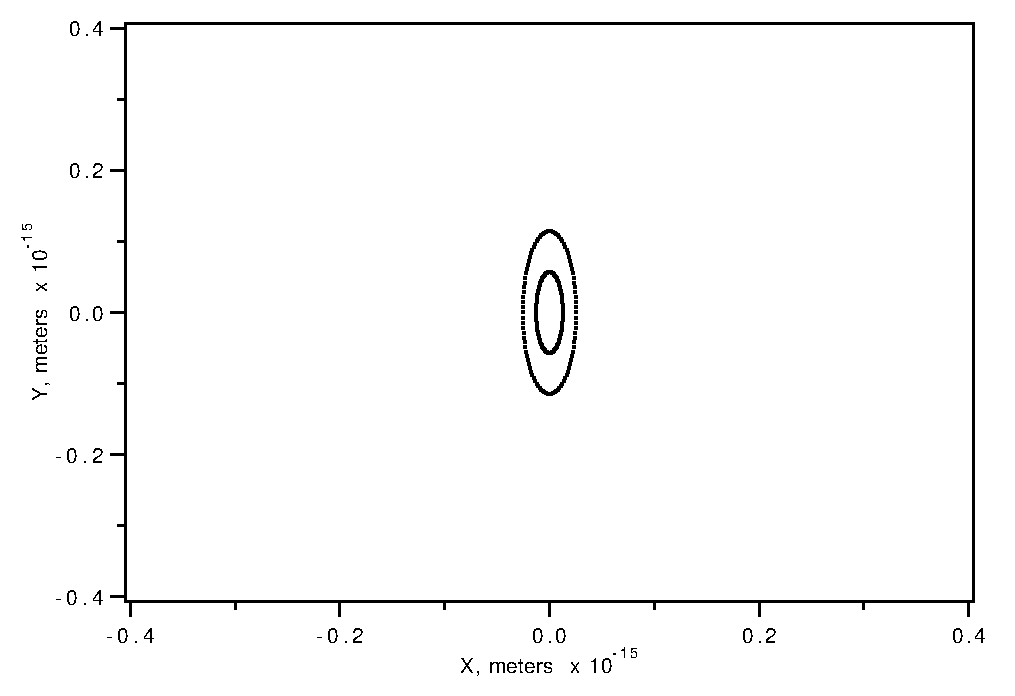
\includegraphics{fig10_3a}
  \caption{Focal spot pattern, for octupole corrected Spot Forming System,
produced by two incoming cylinders of parallel rays.  Third-order single
map calculation.}
\end{figure}

\newpage
\begin{figure}[h]
  \centering
  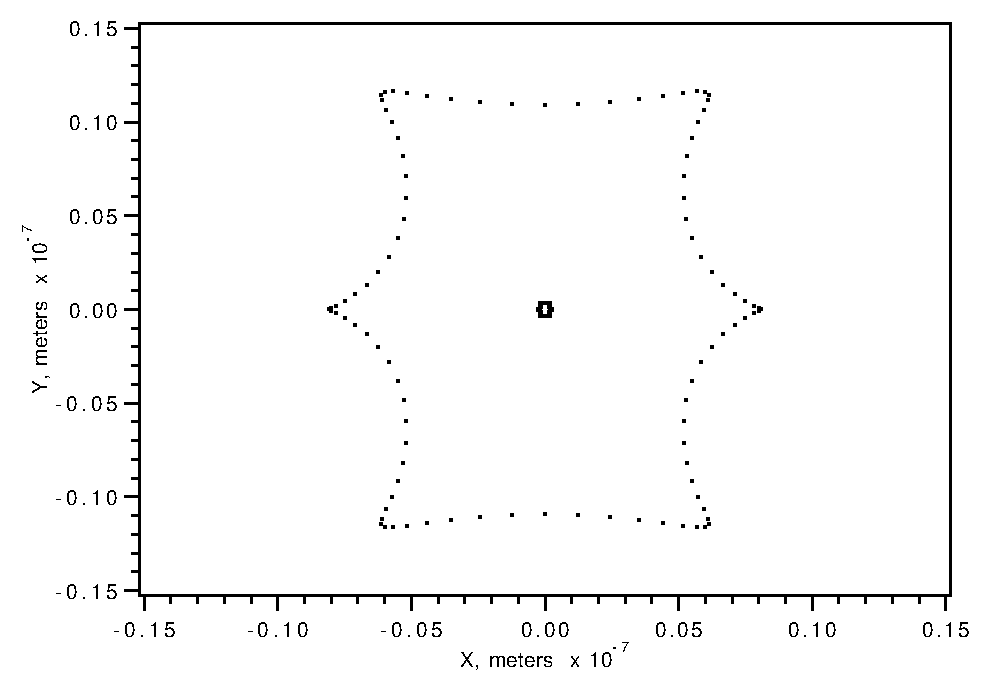
\includegraphics{fig10_3b}
  \caption{Focal spot pattern, for octupole corrected Spot Forming System,
produced by two incoming cylinders of parallel rays.  Third-order
element-by-element calculation.}
\end{figure}
\index{element by element}

\newpage
\subsection{Fitting and Optimizing Seven Octupole Strengths}
\label{seven}
The higher-order aberrations that produce the finite spot size in figure
10.3.1.2 arise from ``cross talk'' between the third-order terms associated
with the hard-edge fringe fields of the quads and the third-order terms
of the various octupoles.  In principle these higher-order terms could be
minimized by the use of more, but {\em weaker}, octupoles.  Ideally one
might consider employing more octupoles with all octupole strengths
adjusted in such a way as to remove detrimental third-order aberrations
while simultaneously minimizing higher-order aberrations.  However,
this cannot be done using \Mary 3.0 since it only computes aberrations
through third-order.  (It can be done with \Mary 5.0.)  What can be done
with \Mary 3.0 is to adjust {\em multiple} octupoles to fit the
detrimental third-order aberrations to zero (as before) while
simultaneously minimizing the sum of the squares of the octupole
strengths.  In so doing, octupole strengths are generally reduced, the
cross talk between them is also reduced, and correspondingly one
might hope that higher-order aberrations are also reduced.\index{fit} \index{optimize} \index{octupole correction} \index{spot forming system}

This is indeed the case.  Exhibit 10.3.2 shows a \Mary run that carries
out the optimization just described.  As before in Exhibit 10.3.1, there
are 3 combined-function quads with octupole components.  In addition, 4
ordinary octupoles are placed around the 3 combined function quadrupoles
in the triplet.  See the contents of the line {\em ctrip} in the
\Mary master input file in Exhibit 10.3.2c.

As illustrated  in Exhibit 10.3.2a, a user-written merit function is
placed in {\em mrt2}.  See section 9.11.  This merit function has access
to the contents of the array {\em ucalc} through use of the include
statement `usrdat.inc'.  The array {\em ucalc} is a multipurpose array.
In this case the first 7 entries of this array are given the values of
the octupole strengths of the 3 combined-function quads and the 4
ordinary octupoles.  This is achieved by the use of a ``vary'' command
with JOB=3 and ISTORE=3 to select the octupole strength parameters of the
three combined function quads and the four octupoles.  See section 9.6.
This ``vary'' command is given the user name {\em selparm} as a mnemonic
for ``select parameters''.  Subsequently a ``wsq'' command with JOB=2,
ISTORE=3,
and IFILE=$-$1 is used to transfer these parameter values to the first
seven storage locations in the array {\em ucalc}.  See section 8.27.
This command is given the user name {\em setucalc}.

The response to the ``vary'' command {\em selparm} described above could
have been made interactively as in Exhibit 10.3.1.  However, it can also
be obtained from an external file.  See section 9.6.  In this example an
external file (file 19) is employed to illustrate use of this feature.
See Exhibit 10.3.2b.

For the \Mary run itself it is necessary to specify what must be fit in
response to the command {\em fitaim} and what must be optimized in
response to the command {\em optaim}.  It is also necessary to specify
what must be varied in response to the commands {\em fitvary} and {\em
optvary}.  See the contents of the lines {\em setup} and {\em work} in
the {\em \#lines} component of the master input file shown in Exhibit
10.3.2g.  The responses to these commands could also have been made
interactively as in Exhibit 10.3.1.  Alternatively, as is done in this
example, they may be provided from external files.  See sections 9.5 and
9.6 and Exhibits 10.3.2c through 10.3.2f.

The desired fitting and optimization are carried out by invoking the line
{\em setup} followed by two {\em nested} logical loops (procedures) in {\em \#labor}.  The
relevant excerpt from {\em \#labor} is shown below:

\begin{center}
setup \\
bop \\
bip \\
clear \\
cspot \\
fit \\
tip \\
work \\
opt \\
top \\
\end{center}

\noindent Fitting is done in an inner procedure which begins with {\em
bip} and terminates with {\em tip}.  Optimization is done in an outer
procedure which begins with {\em bop} and terminates with {\em top}.  See
sections 9.1 through 9.4.

{\bf NOTE WELL}: \ Each procedure (logical loop) must have within it
whatever items are required to compute the quantity that is to be
optimized.  (In this example these items are specified by {\em work}.)  Simply specifying in {\em aim} what is to be optimized is not enough.
There must be items within the logical loop itself that carry out the
necessary associated computations.  Failure to provide these items is a
common mistake for beginning \Mary users.  If the quantity to be optimized
does not actually change during a pass through an optimizing loop (as a result of
failing to compute it or for any other reason) the optimizer terminates with the
error message ``ERROR: \ Faulty Opt Set Up, Aim Space Point NOT Moving!''

Finally, after optimization is complete, one
last fitting procedure is again carried out to ensure that the
detrimental aberrations are indeed completely removed for the current
setting of the four ordinary octupoles.  The relevant
excerpt from {\em \#labor} for this procedure is also shown below:

\begin{center}
work \\
bip \\
clear \\
cspot \\
fit \\
tip \\
\end{center}

By looking at the output of the \Mary run, Exhibit 10.3.2g, one sees that
before optimization (when the ordinary octupoles are off and the octupole
components of the combined function quads have the fitted values found in
Exhibit 10.3.1) the merit function has the value $4.7387 \times
10^{-2}$.  After optimization, when all octupoles are powered, the merit
function has been reduced to the value $3.258891 \times 10^{-2}$.  Does
this optimization actually improve the spot forming performance of the
system?  Figure 10.3.2.1, which should be compared with figure 10.3.1.2, shows
the focal spot pattern for the octupole corrected and optimized Spot
Forming System.  Evidently optimization has reduced the size of the spot
pattern by almost a factor of two.

\begin{footnotesize}
\begin{verbatim}
Exhibit 10.3.2a
Merit function for use by opt:

      subroutine mrt2(p)
c
      include 'impli.inc'
      include 'merit.inc'
      include 'usrdat.inc'
c
c Calling arrays:
      dimension p(6)
c
c set up sum of squares merit function based
c on contents of ucalc
c
c get strengths of octupole components of cfqds
      res1=ucalc(1)
      res2=ucalc(2)
      res3=ucalc(3)
c get strengths of remaining octupoles
      res4=ucalc(4)
      res5=ucalc(5)
      res6=ucalc(6)
      res7=ucalc(7)
c form sum of squares of cfqds octupole strengths
      sscf=res1**2 + res2**2 + res3**2
c form sum of squares of remaining octupole strengths
      sso=res4**2 + res5**2 + res6**2 + res7**2
c form full sum of squares
      sst = sscf + sso
c divide by 7 (the number of octupoles)
      wss = sst/7.d0
c set value of merit function
      val(2)=wss
c
      return
      end


Exhibit 10.3.2b
Contents of file 19 that provides instructions
about what parameters are to be selected in response
to the command selparm:

 parm1      5
 parm2      5
 parm3      5
 oct1       2
 oct2       2
 oct3       2
 oct4       2
  #


Exhibit 10.3.2c
Contents of file 20 that provides instructions
about what aims are to be selected in response
to the command fitaim:

 1    f(140) =      0.000000000E+00
 2    f(149) =      0.000000000E+00
 3    f(195) =      0.000000000E+00
 #


Exhibit 10.3.2d
Contents of file 21 that provides instructions
about what aims are to be selected in response
to the command optaim:

 1       um2 =      0.000000000E+00
 #


Exhibit 10.3.2e
Contents of file 22 that provides instructions
about what parameters are to be selected in response
to the command fitvary:

 parm1      5
 parm2      5
 parm3      5
  #


Exhibit 10.3.2f
Contents of file 23 that provides instructions
about what parameters are to be selected in response
to the command optvary:

 oct1       2
 oct2       2
 oct3       2
 oct4       2
  #

Exhibit 10.3.2g
***MARYLIE 3.0***
Prerelease Development Version 8/21/98
Copyright 1987 Alex J. Dragt
All rights reserved

Data input complete; going into #labor.
#comment
 Exhibit 10.3.2
 This is a MARYLIE run that demonstrates the use of seven octupoles to
 correct three offensive aberrations in the simple spot forming system
 of Section 2.2.  As in Exhibit 10.3.1, each of the three quadrupoles
 also has an octupole component.  In addition, four octupoles are placed
 around the combined function quadrupoles in the triplet.  This run does
 two things:

  a) It adjusts seven octupole strengths to remove ("zero out") three
     Lie generators corresponding to three third-order geometrical
     aberrations that are detrimental to the performance of a
     spot forming system.  These Lie generators are:

     f(140)=f( 04 00 00 ),
     f(149)=f( 02 02 00 ), and
     f(195)=f( 00 04 00 ).

     At the same time the sum of the squares of all seven octupole
     strengths is minimized.  The optimizer is the quadratic step
     optimizer in opt.  This is done by fitting on the octupole strengths
     of the combined function quadrupoles using an inner logical
     loop (procedure) and optimizing on the strengths of the remaining
     four octupoles in an outer procedure.  The merit function used with
     the optimizer is (1/7)*(the sum of the squares of all seven octupole
     strengths).  This quantity is computed in mrt2.  A "vary" command
     (selparm) with ISTORE=3 is used to select the octupole strength
     parameters of the three combined function quads and the four octupoles.
     A "wsq" command (setucalc) with ISTORE=3 and IFILE=-1 is used to
     transfer these selected parameter values to the first 7 storage
     locations in the array ucalc.  The contents of ucalc are used by mrt2
     to compute the merit function.

  b) To give a rough indication of residual fifth-order aberration
     effects, rays are also traced element-by-element through the
     corrected system.  Doing so illustrates as well use of the
     element-by-element tracking ("turtle") feature of MaryLie
     acomplished with the aid of a loop and a 'circ' command.

 The beam parameters are those for 50 MeV protons.

#beam
  1.03527440851950
 5.328901960570000E-002
  1.00000000000000
  1.00000000000000
#menu
 drvs     drft
  0.125000000000000
 drs      drft
  0.500000000000000
 drml     drft
   19.6276000000000
 drl      drft
   20.0026000000000
 cfq1     cfqd
   1.50000000000000       1.00000000000000       1.00000000000000
   1.00000000000000
 cfq2     cfqd
   3.00000000000000       2.00000000000000       1.00000000000000
   1.00000000000000
 cfq3     cfqd
   1.50000000000000       3.00000000000000       1.00000000000000
   1.00000000000000
 oct1     octm
  0.250000000000000      0.000000000000000E+00
 oct2     octm
  0.250000000000000      0.000000000000000E+00
 oct3     octm
  0.250000000000000      0.000000000000000E+00
 oct4     octm
  0.250000000000000      0.000000000000000E+00
 parm1    ps1
  8.630003538054180E-02  0.000000000000000E+00  0.000000000000000E+00
  0.000000000000000E+00 -0.237002616171880      0.000000000000000E+00
 parm2    ps2
 -8.289453107758520E-02  0.000000000000000E+00  0.000000000000000E+00
  0.000000000000000E+00 -3.623291203678830E-02  0.000000000000000E+00
 parm3    ps3
  8.630003538054180E-02  0.000000000000000E+00  0.000000000000000E+00
  0.000000000000000E+00  0.523668825832260      0.000000000000000E+00
 fileout  pmif
   1.00000000000000       12.0000000000000       3.00000000000000
 mapout   ptm
   3.00000000000000       3.00000000000000      0.000000000000000E+00
  0.000000000000000E+00   1.00000000000000
 raysin   rt
   13.0000000000000       14.0000000000000      -1.00000000000000
  0.000000000000000E+00  0.000000000000000E+00  0.000000000000000E+00
 trace14  rt
  0.000000000000000E+00   14.0000000000000       5.00000000000000
   1.00000000000000       1.00000000000000      0.000000000000000E+00
 circ15   circ
  0.000000000000000E+00   15.0000000000000       5.00000000000000
   1.00000000000000       1.00000000000000       3.00000000000000
 clear    iden
 bip      bip
   20.0000000000000
 tip      tip
  0.000000000000000E+00
 bop      bop
   30.0000000000000
 top      top
  0.000000000000000E+00
 selparm  vary
   3.00000000000000       19.0000000000000      0.000000000000000E+00
  0.000000000000000E+00   3.00000000000000      0.000000000000000E+00
 setucalc wsq
   2.00000000000000       3.00000000000000      -1.00000000000000
  0.000000000000000E+00  0.000000000000000E+00  0.000000000000000E+00
 fitaim   aim
   2.00000000000000       20.0000000000000      0.000000000000000E+00
  0.000000000000000E+00   1.00000000000000       1.00000000000000
 optaim   aim
   2.00000000000000       21.0000000000000      0.000000000000000E+00
  0.000000000000000E+00   2.00000000000000       1.00000000000000
 fitvary  vary
   1.00000000000000       22.0000000000000      0.000000000000000E+00
  0.000000000000000E+00   1.00000000000000       1.00000000000000
 optvary  vary
   3.00000000000000       23.0000000000000      0.000000000000000E+00
  0.000000000000000E+00   2.00000000000000       1.00000000000000
 fit      fit
   1.00000000000000      0.000000000000000E+00  1.000000000000000E-10
  1.000000000000000E-04  0.000000000000000E+00   1.00000000000000
 opt      opt
  -11.0000000000000      1.000000000000000E-10  1.000000000000000E-04
  1.000000000000000E-04  0.100000000000000       1.00000000000000
 merit2   mrt2
  0.000000000000000E+00  0.000000000000000E+00  0.000000000000000E+00
  0.000000000000000E+00  0.000000000000000E+00  0.000000000000000E+00
 wmerit2  wmrt
   2.00000000000000       3.00000000000000
 end      end
#lines
 ctrip
     1*oct1        1*drvs        1*cq1         1*drvs        1*oct2     &
     1*drvs        1*cq2         1*drvs        1*oct3        1*drvs     &
     1*cq3         1*drvs        1*oct4
 cspot
     1*ctrip       1*drml
 cq1
     1*parm1       1*cfq1
 cq2
     1*parm2       1*cfq2
 cq3
     1*parm3       1*cfq3
 work
     1*setucalc    1*merit2      1*wmerit2
 setup
     1*selparm     1*work        1*fitaim      1*optaim      1*fitvary  &
     1*optvary
#lumps
#loops
 onebyone
     1*cspot
#labor
    1*fileout
    1*cspot
    1*mapout
    1*setup
    1*bop
    1*bip
    1*clear
    1*cspot
    1*fit
    1*tip
    1*work
    1*opt
    1*top
    1*work
    1*bip
    1*clear
    1*cspot
    1*fit
    1*tip
    1*work
    1*clear
    1*cspot
    1*mapout
    1*fileout
    1*clear
    1*raysin
    1*onebyone
    1*circ15
    1*end

matrix for map is :

-5.66214E-15  2.47288E+01  0.00000E+00  0.00000E+00  0.00000E+00  0.00000E+00
-4.04388E-02  7.93716E-01  0.00000E+00  0.00000E+00  0.00000E+00  0.00000E+00
 0.00000E+00  0.00000E+00 -1.95399E-14  2.28173E+01  0.00000E+00  0.00000E+00
 0.00000E+00  0.00000E+00 -4.38264E-02  8.60207E-01  0.00000E+00  0.00000E+00
 0.00000E+00  0.00000E+00  0.00000E+00  0.00000E+00  1.00000E+00  2.50212E+02
 0.00000E+00  0.00000E+00  0.00000E+00  0.00000E+00  0.00000E+00  1.00000E+00

nonzero elements in generating polynomial are :

 f( 33)=f( 20 00 01 )=-4.67424231122905E-02
 f( 38)=f( 11 00 01 )=  1.4345989929097
 f( 53)=f( 02 00 01 )= -59.832856603695
 f( 67)=f( 00 20 01 )=-0.11069779980158
 f( 70)=f( 00 11 01 )=  4.6810988356401
 f( 76)=f( 00 02 01 )= -88.881855045722
 f( 83)=f( 00 00 03 )= -398.36503473393
 f( 84)=f( 40 00 00 )=-0.12327420824976
 f( 85)=f( 31 00 00 )=  8.7910508067718
 f( 90)=f( 22 00 00 )= -211.07885008368
 f( 95)=f( 20 20 00 )= 0.68595539915843
 f( 96)=f( 20 11 00 )= -25.219718510723
 f( 99)=f( 20 02 00 )=  221.73626436928
 f(104)=f( 20 00 02 )=-0.19664222372908
 f(105)=f( 13 00 00 )=  1706.8172870474
 f(110)=f( 11 20 00 )= -22.188718833104
 f(111)=f( 11 11 00 )=  736.23108430660
 f(114)=f( 11 02 00 )= -5357.5423986589
 f(119)=f( 11 00 02 )=  8.0005227170256
 f(140)=f( 04 00 00 )= 7.62074847671101E-10
 f(145)=f( 02 20 00 )=  139.95819449777
 f(146)=f( 02 11 00 )= -3163.2230792366
 f(149)=f( 02 02 00 )=-5.03137442819934E-09
 f(154)=f( 02 00 02 )= -309.42966067238
 f(175)=f( 00 40 00 )=-9.75409414333912E-02
 f(176)=f( 00 31 00 )=  6.5454816213129
 f(179)=f( 00 22 00 )= -146.85444082834
 f(184)=f( 00 20 02 )=-0.59751982937518
 f(185)=f( 00 13 00 )=  1101.5239192044
 f(190)=f( 00 11 02 )=  32.728267833300
 f(195)=f( 00 04 00 )= 7.92969245821951E-10
 f(200)=f( 00 02 02 )= -601.71802504632
 f(209)=f( 00 00 04 )= -1554.3280602063

***************************************************
* Selection of parameters in response to selparm: *
***************************************************

No.  1 is parm1    ps1     .  Parameter 5 out of 6 selected.
    parm1(5) = -0.23700261617188
No.  2 is parm2    ps2     .  Parameter 5 out of 6 selected.
    parm2(5) = -3.62329120367883E-02
No.  3 is parm3    ps3     .  Parameter 5 out of 6 selected.
    parm3(5) =  0.52366882583226
No.  4 is oct1     octm    .  Parameter 2 out of 2 selected.
     oct1(2) =  0.00000000000000E+00
No.  5 is oct2     octm    .  Parameter 2 out of 2 selected.
     oct2(2) =  0.00000000000000E+00
No.  6 is oct3     octm    .  Parameter 2 out of 2 selected.
     oct3(2) =  0.00000000000000E+00
No.  7 is oct4     octm    .  Parameter 2 out of 2 selected.
     oct4(2) =  0.00000000000000E+00

************************************************
* Value of merit function before optimization: *
************************************************

value of merit function           2 is  4.738744330507415E-002

************************************************************************
* Specifying in fitaim that f(140), f(149), and f(195) should be zero: *
************************************************************************

accept  1:      f(140)
accept  2:      f(149)
accept  3:      f(195)

 Aims selected :
No.     item        present value        target value
----------------------------------------------------
 1    f(140) =      7.620748477E-10     0.000000000E+00
 2    f(149) =     -5.031374428E-09     0.000000000E+00
 3    f(195) =      7.929692458E-10     0.000000000E+00

***************************************************************************
* Specifying in optaim that um2, the merit function, should be minimized: *
***************************************************************************

accept  1:         um2

 Aims selected :
No.     item        present value        target value
----------------------------------------------------
 1       um2 =      4.738744331E-02     0.000000000E+00


**********************************************************
* Specifying in fitvary that the fifth parameters in the *
* parameter sets 1 through 3 should be varied by fit:    *
**********************************************************

No.  1 is parm1    ps1     .  Parameter 5 out of 6 selected.
    parm1(5) = -0.23700261617188
No.  2 is parm2    ps2     .  Parameter 5 out of 6 selected.
    parm2(5) = -3.62329120367883E-02
No.  3 is parm3    ps3     .  Parameter 5 out of 6 selected.
    parm3(5) =  0.52366882583226

  Variable #menu elements selected:
No.  Element    Type     Parameter   Present value
-----------------------------------------------------------
 1    parm1      ps1          5     -0.23700261617188
 2    parm2      ps2          5     -3.62329120367883E-02
 3    parm3      ps3          5      0.52366882583226

****************************************************************
* Specifying in optvary that the second parameters in the      *
* octupole elements oct1 through oct4 should be varied by opt: *
****************************************************************

No.  1 is oct1     octm    .  Parameter 2 out of 2 selected.
     oct1(2) =  0.00000000000000E+00
No.  2 is oct2     octm    .  Parameter 2 out of 2 selected.
     oct2(2) =  0.00000000000000E+00
No.  3 is oct3     octm    .  Parameter 2 out of 2 selected.
     oct3(2) =  0.00000000000000E+00
No.  4 is oct4     octm    .  Parameter 2 out of 2 selected.
     oct4(2) =  0.00000000000000E+00

  Variable #menu elements selected:
No.  Element    Type     Parameter   Present value
-----------------------------------------------------------
 1    oct1       octm         2      0.00000000000000E+00
 2    oct2       octm         2      0.00000000000000E+00
 3    oct3       octm         2      0.00000000000000E+00
 4    oct4       octm         2      0.00000000000000E+00

**************************************************
* Beginning of fitting and optimization process: *
**************************************************

**************************
* First fitting process: *
**************************

 target           1 =  0.000000000000000E+000
 target           2 =  0.000000000000000E+000
 target           3 =  0.000000000000000E+000
Iter   1 Error= 5.0314E-09,  Step=-2.3700E-05,  SubErr= 5.0314E-09 @cut=    1
-------------------------------------------------------
Iter   2 Error= 1.6360E+01,  Step=-3.6233E-06,  SubErr= 1.6360E+01 @cut=    1
-------------------------------------------------------
Iter   3 Error= 4.2241E+00,  Step= 5.2367E-05,  SubErr= 4.2241E+00 @cut=    1
-------------------------------------------------------
Iter   4 Error= 2.1115E+01,  Step= 5.2367E-05,  SubErr= 2.1115E+01 @cut=    1
-------------------------------------------------------
Iter   5 Error= 2.7610E-10,  Step= 5.6728E-15,  SubErr= 2.7610E-10 @cut=    1
-------------------------------------------------------
Quit on iteration   6 for reason 1: Converged: error < tolerance
Final values with reach =   1 are:

 Aims selected :
No.     item        present value        target value
----------------------------------------------------
 1    f(140) =     -2.355804440E-11     0.000000000E+00
 2    f(149) =     -3.358735512E-11     0.000000000E+00
 3    f(195) =     -9.745093621E-12     0.000000000E+00

 New values for parameters:
No.  Element    Type   Parameter   Present value         IDV  Slope
-----------------------------------------------------------------------
 1   parm1      ps1        5     -0.23700261617188
 2   parm2      ps2        5     -3.62329120367892E-02
 3   parm3      ps3        5      0.52366882583228

 Maximum error is     3.358736E-11
 Maximum allowed was  1.000000E-10
value of merit function           2 is  4.738744330507717E-002

**************************************
* Beginning of optimization process: *
**************************************

 OPT is initialized

   1=iter   F=  4.738744330508E-02  DF=  4.738744E-02  DX=  4.072297E-02
XNEW:  -8.0554614611E-02 -9.2573944632E-02 -0.1525865604      4.0722971665E-02
-------------------------------------------------------

***************************
* Second fitting process: *
***************************

 target           1 =  0.000000000000000E+000
 target           2 =  0.000000000000000E+000
 target           3 =  0.000000000000000E+000
Iter   1 Error= 2.9632E+04,  Step=-2.3700E-05,  SubErr= 2.9632E+04 @cut=    1
-------------------------------------------------------
Iter   2 Error= 2.9648E+04,  Step=-3.6233E-06,  SubErr= 2.9648E+04 @cut=    1
-------------------------------------------------------
Iter   3 Error= 2.9636E+04,  Step= 5.2367E-05,  SubErr= 2.9636E+04 @cut=    1
-------------------------------------------------------
Iter   4 Error= 2.9611E+04,  Step= 6.2288E-02,  SubErr= 2.9611E+04 @cut=    1
-------------------------------------------------------
Iter   5 Error= 2.5191E-07,  Step= 4.1437E-12,  SubErr= 2.5191E-07 @cut=    1
-------------------------------------------------------
Iter   6 Error= 1.7298E-10,  Step= 1.5157E-14,  SubErr= 1.7298E-10 @cut=    1
-------------------------------------------------------
Quit on iteration   7 for reason 1: Converged: error < tolerance
Final values with reach =   1 are:

 Aims selected :
No.     item        present value        target value
----------------------------------------------------
 1    f(140) =      1.481126333E-11     0.000000000E+00
 2    f(149) =      1.996625087E-12     0.000000000E+00
 3    f(195) =     -1.997690902E-11     0.000000000E+00

 New values for parameters:
No.  Element    Type   Parameter   Present value         IDV  Slope
-----------------------------------------------------------------------
 1   parm1      ps1        5     -0.23860001986872
 2   parm2      ps2        5     -3.13582643927528E-02
 3   parm3      ps3        5      0.58579797083584

 Maximum error is     1.997691E-11
 Maximum allowed was  1.000000E-10
value of merit function           2 is  6.301036755178095E-002

**************************************
* Second pass through the optimizer: *
**************************************


   2=iter   F=  6.301036755178E-02  DF=  1.562292E-02  DX=  9.026208E-02
XNEW:   0.1203632232     -9.0738312807E-02 -1.1053048434E-02  0.1309850496
-------------------------------------------------------

**************************
* Third fitting process: *
**************************

 target           1 =  0.000000000000000E+000
 target           2 =  0.000000000000000E+000
 target           3 =  0.000000000000000E+000
Iter   1 Error= 3.9617E+04,  Step=-2.3860E-05,  SubErr= 3.9617E+04 @cut=    1
-------------------------------------------------------
Iter   2 Error= 3.9601E+04,  Step=-3.1358E-06,  SubErr= 3.9601E+04 @cut=    1
-------------------------------------------------------
Iter   3 Error= 3.9613E+04,  Step= 5.8580E-05,  SubErr= 3.9613E+04 @cut=    1
-------------------------------------------------------
Iter   4 Error= 3.9641E+04,  Step= 5.6977E-02,  SubErr= 3.9641E+04 @cut=    1
-------------------------------------------------------
Iter   5 Error= 2.0548E-07,  Step= 1.2945E-12,  SubErr= 2.0548E-07 @cut=    1
-------------------------------------------------------
Iter   6 Error= 1.0396E-10,  Step= 5.0826E-15,  SubErr= 1.0396E-10 @cut=    1
-------------------------------------------------------
Quit on iteration   7 for reason 1: Converged: error < tolerance
Final values with reach =   1 are:

 Aims selected :
No.     item        present value        target value
----------------------------------------------------
 1    f(140) =      3.413802574E-11     0.000000000E+00
 2    f(149) =     -6.007638831E-11     0.000000000E+00
 3    f(195) =     -2.334488158E-11     0.000000000E+00

 New values for parameters:
No.  Element    Type   Parameter   Present value         IDV  Slope
-----------------------------------------------------------------------
 1   parm1      ps1        5     -0.29476105240516
 2   parm2      ps2        5     -3.51579943703615E-02
 3   parm3      ps3        5      0.59467937850852

 Maximum error is     6.007639E-11
 Maximum allowed was  1.000000E-10
value of merit function           2 is  6.882338940091765E-002

******************
* ETC, ETC, ETC. *
******************

  14=iter   F=  3.260264197907E-02  DF= -5.341392E-05  DX=  8.732209E-04
XNEW:  -0.1521671061      0.1813548907      0.1214744146      1.1100786946E-02
-------------------------------------------------------

***********************************************************
* Last fitting process in optimization-fitting procedure: *
***********************************************************


 target           1 =  0.000000000000000E+000
 target           2 =  0.000000000000000E+000
 target           3 =  0.000000000000000E+000
Iter   1 Error= 1.3272E+03,  Step=-1.5708E-05,  SubErr= 1.3272E+03 @cut=    1
-------------------------------------------------------
Iter   2 Error= 1.3380E+03,  Step=-4.0540E-06,  SubErr= 1.3380E+03 @cut=    1
-------------------------------------------------------
Iter   3 Error= 1.3319E+03,  Step= 3.6328E-05,  SubErr= 1.3319E+03 @cut=    1
-------------------------------------------------------
Iter   4 Error= 1.3125E+03,  Step= 2.2521E-03,  SubErr= 1.3125E+03 @cut=    1
-------------------------------------------------------
Iter   5 Error= 9.6571E-09,  Step= 1.0386E-12,  SubErr= 9.6571E-09 @cut=    1
-------------------------------------------------------
Quit on iteration   6 for reason 1: Converged: error < tolerance
Final values with reach =   1 are:

 Aims selected :
No.     item        present value        target value
----------------------------------------------------
 1    f(140) =      8.177281074E-11     0.000000000E+00
 2    f(149) =      8.237321936E-11     0.000000000E+00
 3    f(195) =      1.004352157E-11     0.000000000E+00

 New values for parameters:
No.  Element    Type   Parameter   Present value         IDV  Slope
-----------------------------------------------------------------------
 1   parm1      ps1        5     -0.15490720001740
 2   parm2      ps2        5     -4.04928706913628E-02
 3   parm3      ps3        5      0.36271588688665

 Maximum error is     8.237322E-11
 Maximum allowed was  1.000000E-10
value of merit function           2 is  3.258891617766553E-002

************************************
* Last pass through the optimizer: *
************************************

  15=iter   F=  3.258891617767E-02  DF= -1.372580E-05  DX=  7.954995E-05
XNEW:  -0.1522469818      0.1813821208      0.1213325660      1.1180336891E-02
-------------------------------------------------------

done
relative gradient is less than gtol.
After   15 total iterations, final values are:
Final RMS error for loop 2 is  3.2588916178E-02

 New values for parameters:
No.  Element    Type   Parameter   Present value         IDV  Slope
-----------------------------------------------------------------------
 1   oct1       octm       2     -0.15224698182631
 2   oct2       octm       2      0.18138212079769
 3   oct3       octm       2      0.12133256602590
 4   oct4       octm       2      1.11803368908222E-02

 Final change was -1.372580E-05  final step was  7.954995E-05
 Tolerances: ftol= 1.000000E-10            xtol= 1.000000E-04
value of merit function           2 is  3.258913378939155E-002

***********************************************
* Final fitting procedure after optimization: *
***********************************************

 target           1 =  0.000000000000000E+000
 target           2 =  0.000000000000000E+000
 target           3 =  0.000000000000000E+000
Iter   1 Error= 1.3039E+01,  Step=-1.5491E-05,  SubErr= 1.3039E+01 @cut=    1
-------------------------------------------------------
Iter   2 Error= 2.3733E+01,  Step=-4.0493E-06,  SubErr= 2.3733E+01 @cut=    1
-------------------------------------------------------
Iter   3 Error= 1.7760E+01,  Step= 3.6272E-05,  SubErr= 1.7760E+01 @cut=    1
-------------------------------------------------------
Iter   4 Error= 1.5858E+00,  Step= 3.5221E-05,  SubErr= 1.5858E+00 @cut=    1
-------------------------------------------------------
Quit on iteration   5 for reason 1: Converged: error < tolerance
Final values with reach =   1 are:

 Aims selected :
No.     item        present value        target value
----------------------------------------------------
 1    f(140) =     -9.404033108E-12     0.000000000E+00
 2    f(149) =      1.063682475E-11     0.000000000E+00
 3    f(195) =     -1.996980359E-11     0.000000000E+00

 New values for parameters:
No.  Element    Type   Parameter   Present value         IDV  Slope
-----------------------------------------------------------------------
 1   parm1      ps1        5     -0.15489553304785
 2   parm2      ps2        5     -4.04896976522865E-02
 3   parm3      ps3        5      0.36271907726308

 Maximum error is     1.996980E-11
 Maximum allowed was  1.000000E-10

*********************************************************************
* Final value of merit function for optimized and corrected system: *
*********************************************************************

value of merit function           2 is  3.258891135949125E-002

*****************************************************************
* Transfer map for optimized and corrected Spot Forming System: *
*****************************************************************

matrix for map is :

-5.66214E-15  2.47288E+01  0.00000E+00  0.00000E+00  0.00000E+00  0.00000E+00
-4.04388E-02  7.93716E-01  0.00000E+00  0.00000E+00  0.00000E+00  0.00000E+00
 0.00000E+00  0.00000E+00 -1.95399E-14  2.28173E+01  0.00000E+00  0.00000E+00
 0.00000E+00  0.00000E+00 -4.38264E-02  8.60207E-01  0.00000E+00  0.00000E+00
 0.00000E+00  0.00000E+00  0.00000E+00  0.00000E+00  1.00000E+00  2.50212E+02
 0.00000E+00  0.00000E+00  0.00000E+00  0.00000E+00  0.00000E+00  1.00000E+00

nonzero elements in generating polynomial are :

 f( 33)=f( 20 00 01 )=-4.67424231122905E-02
 f( 38)=f( 11 00 01 )=  1.4345989929097
 f( 53)=f( 02 00 01 )= -59.832856603695
 f( 67)=f( 00 20 01 )=-0.11069779980158
 f( 70)=f( 00 11 01 )=  4.6810988356401
 f( 76)=f( 00 02 01 )= -88.881855045722
 f( 83)=f( 00 00 03 )= -398.36503473393
 f( 84)=f( 40 00 00 )=-8.89083353541492E-02
 f( 85)=f( 31 00 00 )=  6.3613003164667
 f( 90)=f( 22 00 00 )= -153.33711587259
 f( 95)=f( 20 20 00 )= 0.49139317427674
 f( 96)=f( 20 11 00 )= -18.071264442261
 f( 99)=f( 20 02 00 )=  158.73936098854
 f(104)=f( 20 00 02 )=-0.19664222372908
 f(105)=f( 13 00 00 )=  1245.5445056207
 f(110)=f( 11 20 00 )= -15.974726045653
 f(111)=f( 11 11 00 )=  530.15850256210
 f(114)=f( 11 02 00 )= -3846.3731133617
 f(119)=f( 11 00 02 )=  8.0005227170256
 f(140)=f( 04 00 00 )=-9.40403310778493E-12
 f(145)=f( 02 20 00 )=  101.88774855927
 f(146)=f( 02 11 00 )= -2311.9488850312
 f(149)=f( 02 02 00 )= 1.06368247543287E-11
 f(154)=f( 02 00 02 )= -309.42966067238
 f(175)=f( 00 40 00 )=-6.95583699768062E-02
 f(176)=f( 00 31 00 )=  4.6744564689799
 f(179)=f( 00 22 00 )= -105.05879704592
 f(184)=f( 00 20 02 )=-0.59751982937518
 f(185)=f( 00 13 00 )=  789.61713892920
 f(190)=f( 00 11 02 )=  32.728267833300
 f(195)=f( 00 04 00 )=-1.99698035885376E-11
 f(200)=f( 00 02 02 )= -601.71802504632
 f(209)=f( 00 00 04 )= -1554.3280602063

*************************************
* Writing out new master input file *
* with optimized parameter values:  *
*************************************

#comment
 Exhibit 10.3.2
 This is a MARYLIE run that demonstrates the use of seven octupoles to
 correct three offensive aberrations in the simple spot forming system
 of Section 2.2.  As in Exhibit 10.3.1, each of the three quadrupoles
 also has an octupole component.  In addition, four octupoles are placed
 around the combined function quadrupoles in the triplet.  This run does
 two things:

  a) It adjusts seven octupole strengths to remove ("zero out") three
     Lie generators corresponding to three third-order geometrical
     aberrations that are detrimental to the performance of a
     spot forming system.  These Lie generators are:

     f(140)=f( 04 00 00 ),
     f(149)=f( 02 02 00 ), and
     f(195)=f( 00 04 00 ).

     At the same time the sum of the squares of all seven octupole
     strengths is minimized.  The optimizer is the quadratic step
     optimizer in opt.  This is done by fitting on the octupole strengths
     of the combined function quadrupoles using an inner logical
     loop (procedure) and optimizing on the strengths of the remaining
     four octupoles in an outer procedure.  The merit function used with
     the optimizer is (1/7)*(the sum of the squares of all seven octupole
     strengths).  This quantity is computed in mrt2.  A "vary" command
     (selparm) with ISTORE=3 is used to select the octupole strength
     parameters of the three combined function quads and the four octupoles.
     A "wsq" command (setucalc) with ISTORE=3 and IFILE=-1 is used to
     transfer these selected parameter values to the first 7 storage
     locations in the array ucalc.  The contents of ucalc are used by mrt2
     to compute the merit function.

  b) To give a rough indication of residual fifth-order aberration
     effects, rays are also traced element-by-element through the
     corrected system.  Doing so illustrates as well use of the
     element-by-element tracking ("turtle") feature of MaryLie
     acomplished with the aid of a loop and a 'circ' command.

 The beam parameters are those for 50 MeV protons.

#beam
  1.03527440851950
 5.328901960570000E-002
  1.00000000000000
  1.00000000000000
#menu
 drvs     drft
  0.125000000000000
 drs      drft
  0.500000000000000
 drml     drft
   19.6276000000000
 drl      drft
   20.0026000000000
 cfq1     cfqd
   1.50000000000000       1.00000000000000       1.00000000000000
   1.00000000000000
 cfq2     cfqd
   3.00000000000000       2.00000000000000       1.00000000000000
   1.00000000000000
 cfq3     cfqd
   1.50000000000000       3.00000000000000       1.00000000000000
   1.00000000000000
 oct1     octm
  0.250000000000000     -0.152246981826309
 oct2     octm
  0.250000000000000      0.181382120797693
 oct3     octm
  0.250000000000000      0.121332566025899
 oct4     octm
  0.250000000000000      1.118033689082220E-02
 parm1    ps1
  8.630003538054180E-02  0.000000000000000E+00  0.000000000000000E+00
  0.000000000000000E+00 -0.154895533047847      0.000000000000000E+00
 parm2    ps2
 -8.289453107758520E-02  0.000000000000000E+00  0.000000000000000E+00
  0.000000000000000E+00 -4.048969765228652E-02  0.000000000000000E+00
 parm3    ps3
  8.630003538054180E-02  0.000000000000000E+00  0.000000000000000E+00
  0.000000000000000E+00  0.362719077263076      0.000000000000000E+00
 fileout  pmif
   1.00000000000000       12.0000000000000       3.00000000000000
 mapout   ptm
   3.00000000000000       3.00000000000000      0.000000000000000E+00
  0.000000000000000E+00   1.00000000000000
 raysin   rt
   13.0000000000000       14.0000000000000      -1.00000000000000
  0.000000000000000E+00  0.000000000000000E+00  0.000000000000000E+00
 trace14  rt
  0.000000000000000E+00   14.0000000000000       5.00000000000000
   1.00000000000000       1.00000000000000      0.000000000000000E+00
 circ15   circ
  0.000000000000000E+00   15.0000000000000       5.00000000000000
   1.00000000000000       1.00000000000000       3.00000000000000
 clear    iden
 bip      bip
   20.0000000000000
 tip      tip
  0.000000000000000E+00
 bop      bop
   30.0000000000000
 top      top
  0.000000000000000E+00
 selparm  vary
   3.00000000000000       19.0000000000000      0.000000000000000E+00
  0.000000000000000E+00   3.00000000000000      0.000000000000000E+00
 setucalc wsq
   2.00000000000000       3.00000000000000      -1.00000000000000
  0.000000000000000E+00  0.000000000000000E+00  0.000000000000000E+00
 fitaim   aim
   2.00000000000000       20.0000000000000      0.000000000000000E+00
  0.000000000000000E+00   1.00000000000000       1.00000000000000
 optaim   aim
   2.00000000000000       21.0000000000000      0.000000000000000E+00
  0.000000000000000E+00   2.00000000000000       1.00000000000000
 fitvary  vary
   1.00000000000000       22.0000000000000      0.000000000000000E+00
  0.000000000000000E+00   1.00000000000000       1.00000000000000
 optvary  vary
   3.00000000000000       23.0000000000000      0.000000000000000E+00
  0.000000000000000E+00   2.00000000000000       1.00000000000000
 fit      fit
   1.00000000000000      0.000000000000000E+00  1.000000000000000E-10
  1.000000000000000E-04  0.000000000000000E+00   1.00000000000000
 opt      opt
  -11.0000000000000      1.000000000000000E-10  1.000000000000000E-04
  1.000000000000000E-04  0.100000000000000       1.00000000000000
 merit2   mrt2
  0.000000000000000E+00  0.000000000000000E+00  0.000000000000000E+00
  0.000000000000000E+00  0.000000000000000E+00  0.000000000000000E+00
 wmerit2  wmrt
   2.00000000000000       3.00000000000000
 end      end
#lines
 ctrip
     1*oct1        1*drvs        1*cq1         1*drvs        1*oct2     &
     1*drvs        1*cq2         1*drvs        1*oct3        1*drvs     &
     1*cq3         1*drvs        1*oct4
 cspot
     1*ctrip       1*drml
 cq1
     1*parm1       1*cfq1
 cq2
     1*parm2       1*cfq2
 cq3
     1*parm3       1*cfq3
 work
     1*setucalc    1*merit2      1*wmerit2
 setup
     1*selparm     1*work        1*fitaim      1*optaim      1*fitvary  &
     1*optvary
#lumps
#loops
 onebyone
     1*cspot
#labor
    1*fileout
    1*cspot
    1*mapout
    1*setup
    1*bop
    1*bip
    1*clear
    1*cspot
    1*fit
    1*tip
    1*work
    1*opt
    1*top
    1*work
    1*bip
    1*clear
    1*cspot
    1*fit
    1*tip
    1*work
    1*clear
    1*cspot
    1*mapout
    1*fileout
    1*clear
    1*raysin
    1*onebyone
    1*circ15
    1*end

*********************************
* Element-by element ray trace: *
*********************************

  200 ray(s) read in from file  13
circulating through onebyone :
 oct1     drvs     parm1    cfq1     drvs
 oct2     drvs     parm2    cfq2     drvs
 oct3     drvs     parm3    cfq3     drvs
 oct4     drml

end of MARYLIE run
\end{verbatim}
\end{footnotesize}

\newpage
\renewcommand{\thefigure}{\thesubsection.\arabic{figure}}
%\setcounter{\thefigure}{1}
\begin{figure}[h]
  \centering
  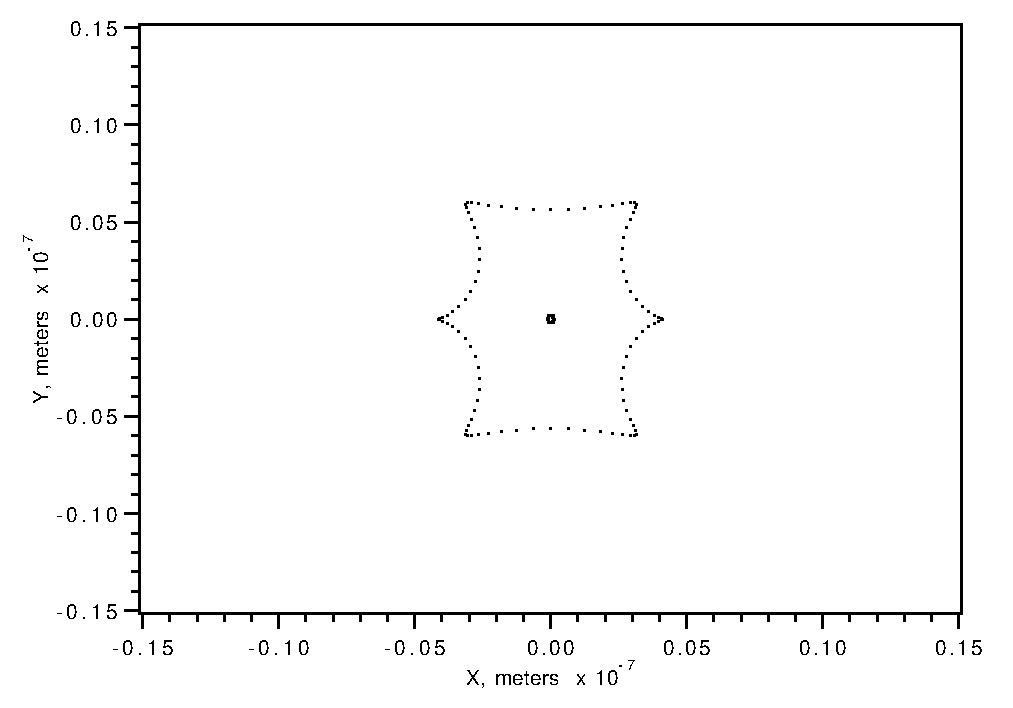
\includegraphics{fig10_3c}
  \caption{Focal spot pattern, for octupole corrected and optimized Spot Forming System,
produced by two incoming cylinders of parallel rays.  Third-order
element-by-element calculation.}
\end{figure}
\index{element by element}

\subsection{Optimizing Using the MSS Optimizer} \index{optimize} \index{MSS optimizer}
\label{mss}
Since the merit function in the last example was a sum of squares, see
Exhibit 10.3.2a, it is tempting to carry out optimization using the
nonlinear least squares optimizer in {\em mss} that is designed for this
purpose (see section 9.8) rather than {\em opt}.  Exhibits 10.3.3a and
10.3.3b describe a
\Mary run that carries out this alternate approach.  As before external
files 19, 20, 22, and 23, that are identical to those shown in Exhibits
10.3.2b, 10.3.2c, 10.3.2e, and 10.3.2f, respectively, are used to respond
to the commands {\em selparm}, {\em fitaim}, {\em fitvary}, and {\em
optvary}, respectively.  In particular, the contents of {\em ucalc} are
established as before.  However, the response to {\em optaim}, given by
the contents of file 21, differs as shown in Exhibit 10.3.3a.  Now the
weighted sum of squares merit function is set up directly from the
contents of {\em ucalc} by {\em optaim} using JOB=3.  (The optimizer {\em
mss} requires that a weighted sum of squares merit function be set up in
{\em aim} because it makes use of the ingredients of the merit function
as well as its total value.)  See sections 9.5, 9.8, and 9.10.

Exhibit 10.3.b shows the \Mary run itself.  Evidently the final fitted
and optimized octupole values are essentially identical to those found in
Exhibit 10.3.2f.  However, only 6 passes through the {\em mss} optimizer
were required in contrast to the 15 passes through {\em opt} in Exhibit
10.3.2f.  We conclude that, at least for this example, the nonlinear
least squares optimizer in {\em mss} is indeed superior when the merit
function is a weighted sum of squares.

{\bf NOTE WELL}: \ Each procedure (logical loop) must have within it
whatever items are required to compute the quantities that are to be
optimized.  (In this example these items are specified by {\em work}.)  Simply specifying in {\em aim} what is to be optimized is not enough.
There must be items within the logical loop itself that carry out the
necessary associated computations.  Failure to provide these items is a
common mistake for beginning \Mary users.  If the quantity to be optimized
does
not actually change during a pass through a optimizing loop (as a result of
failing to compute it or for any other reason) the optimizer terminates with the
error message ``ERROR: \ Faulty Mss Set Up, Aim Space Point NOT Moving!''

Two comments, one about programming and one about physics, can be made at
this point.  With regard to programming, if one is content to use
weighted-sum-of-squares merit functions, then they can always be set up
for use with either {\em mss} or {\em opt} simply by using {\em aim} with
JOB=3 as was done in this example.  That is, there is then no need to
write merit function
routines as in Exhibit 10.3.2a.  See sections 9.5 and 9.9.  With regard
to physics, it is evident from Exhibits 10.3.2g and 10.3.3b that, after
optimization (sum of squares minimization), the octupole strengths of
cfqd2 and oct4 are rather small compared to the others.  This suggests
these elements are rather {\em ineffective} as correctors.  (After sum-of-squares
minimization, correctors with large strengths must be effective since
there would be otherwise no reason for them to be large considering that
their large values have the undesirable feature of making the
sum-of-squares merit function large.  Correspondingly, weak correctors
must be ineffective.)  Consequently, it would be worth exploring the
optimized solution when only 5 octupole correctors (those in cdqd1 and
cfqd3 and oct1, oct2, and oct3) are used.  This solution is likely to be
almost as good as that with 7 octupole correctors.

\begin{footnotesize}
\begin{verbatim}
Exhibit 10.3.3a
Contents of file 21 that provides instructions
about what aims are to be selected in response
to the command optaim:

 1    u(  1) =      0.000000000E+00      1.00000000
 2    u(  2) =      0.000000000E+00      1.00000000
 3    u(  3) =      0.000000000E+00      1.00000000
 4    u(  4) =      0.000000000E+00      1.00000000
 5    u(  5) =      0.000000000E+00      1.00000000
 6    u(  6) =      0.000000000E+00      1.00000000
 7    u(  7) =      0.000000000E+00      1.00000000
 #

Exhibit 10.3.3b
***MARYLIE 3.0***
Prerelease Development Version 1/12/00
Copyright 1987 Alex J. Dragt
All rights reserved

Data input complete; going into #labor.
#comment
 Exhibit 10.3.3
 This is a MARYLIE run that demonstrates the use of seven octupoles to
 correct three offensive aberrations in the simple spot forming system
 of Section 2.2.  It is similar to that in Exhibit 10.3.2 except that
 the sum of squares merit function is set up in aim and the mss optimizer
 is used in place of opt.  Specifically, this run adjusts seven octupole
 strengths to remove ("zero out") three Lie generators corresponding to
 three third-order geometrical aberrations that are detrimental to the
 performance of a spot forming system.  These Lie generators are:

     f(140)=f( 04 00 00 ),
     f(149)=f( 02 02 00 ), and
     f(195)=f( 00 04 00 ).

 At the same time the sum of the squares of all seven octupole
 strengths is minimized.  The optimizer is the nonlinear least squares
 optimizer in mss.  As in Exhibit 10.3.2, this is done by fitting on
 the octupole strengths of the combined function quadrupoles using an
 inner logical loop (procedure) and optimizing on the strengths of the
 remaining four octupoles in an outer procedure.  A "vary" command
 (selparm) with ISTORE=3 is used to select the octupole strength parameters
 of the three combined function quads and the four octupoles.  A "wsq"
 command (setucalc) with ISTORE=3 and IFILE=-1 is used to transfer these
 selected parameter values to the first 7 storage locations in the array
 ucalc.  A merit function, which is again (1/7)*(the sum of the squares of
 all seven octupole strengths) and is available as mrt0, is set up in optaim
 (with JOB=3) based on the entries in ucalc.

 The beam parameters are those for 50 MeV protons.

#beam
  1.03527440851950
 5.328901960570000E-002
  1.00000000000000
  1.00000000000000
#menu
 drvs     drft
  0.125000000000000
 drs      drft
  0.500000000000000
 drml     drft
   19.6276000000000
 drl      drft
   20.0026000000000
 cfq1     cfqd
   1.50000000000000       1.00000000000000       1.00000000000000
   1.00000000000000
 cfq2     cfqd
   3.00000000000000       2.00000000000000       1.00000000000000
   1.00000000000000
 cfq3     cfqd
   1.50000000000000       3.00000000000000       1.00000000000000
   1.00000000000000
 oct1     octm
  0.250000000000000      0.000000000000000E+00
 oct2     octm
  0.250000000000000      0.000000000000000E+00
 oct3     octm
  0.250000000000000      0.000000000000000E+00
 oct4     octm
  0.250000000000000      0.000000000000000E+00
 parm1    ps1
  8.630003538054180E-02  0.000000000000000E+00  0.000000000000000E+00
  0.000000000000000E+00 -0.237002616171880      0.000000000000000E+00
 parm2    ps2
 -8.289453107758520E-02  0.000000000000000E+00  0.000000000000000E+00
  0.000000000000000E+00 -3.623291203678830E-02  0.000000000000000E+00
 parm3    ps3
  8.630003538054180E-02  0.000000000000000E+00  0.000000000000000E+00
  0.000000000000000E+00  0.523668825832260      0.000000000000000E+00
 fileout  pmif
   1.00000000000000       12.0000000000000       3.00000000000000
 mapout   ptm
   3.00000000000000       3.00000000000000      0.000000000000000E+00
  0.000000000000000E+00   1.00000000000000
 raysin   rt
   13.0000000000000       14.0000000000000      -1.00000000000000
  0.000000000000000E+00  0.000000000000000E+00  0.000000000000000E+00
 trace14  rt
  0.000000000000000E+00   14.0000000000000       5.00000000000000
   1.00000000000000       1.00000000000000      0.000000000000000E+00
 circ15   circ
  0.000000000000000E+00   15.0000000000000       5.00000000000000
   1.00000000000000       1.00000000000000       3.00000000000000
 clear    iden
 bip      bip
   20.0000000000000
 tip      tip
  0.000000000000000E+00
 bop      bop
   30.0000000000000
 top      top
  0.000000000000000E+00
 selparm  vary
   3.00000000000000       19.0000000000000      0.000000000000000E+00
  0.000000000000000E+00   3.00000000000000      0.000000000000000E+00
 setucalc wsq
   2.00000000000000       3.00000000000000      -1.00000000000000
  0.000000000000000E+00  0.000000000000000E+00  0.000000000000000E+00
 fitaim   aim
   2.00000000000000       20.0000000000000      0.000000000000000E+00
  0.000000000000000E+00   1.00000000000000       1.00000000000000
 optaim   aim
   3.00000000000000       21.0000000000000      0.000000000000000E+00
  0.000000000000000E+00   2.00000000000000       1.00000000000000
 fitvary  vary
   1.00000000000000       22.0000000000000      0.000000000000000E+00
  0.000000000000000E+00   1.00000000000000       1.00000000000000
 optvary  vary
   3.00000000000000       23.0000000000000      0.000000000000000E+00
  0.000000000000000E+00   2.00000000000000       1.00000000000000
 fit      fit
   1.00000000000000      0.000000000000000E+00  1.000000000000000E-10
  1.000000000000000E-04  0.000000000000000E+00   1.00000000000000
 mss      mss
  -1.00000000000000      1.000000000000000E-10  1.000000000000000E-04
  1.000000000000000E-04  0.100000000000000       1.00000000000000
 merit0   mrt0
   1.00000000000000       2.00000000000000
 wmerit0  wmrt
  0.000000000000000E+00   3.00000000000000
 merit2   mrt2
  0.000000000000000E+00  0.000000000000000E+00  0.000000000000000E+00
  0.000000000000000E+00  0.000000000000000E+00  0.000000000000000E+00
 wmerit2  wmrt
   2.00000000000000       3.00000000000000
 end      end
#lines
 ctrip
     1*oct1        1*drvs        1*cq1         1*drvs        1*oct2     &
     1*drvs        1*cq2         1*drvs        1*oct3        1*drvs     &
     1*cq3         1*drvs        1*oct4
 cspot
     1*ctrip       1*drml
 cq1
     1*parm1       1*cfq1
 cq2
     1*parm2       1*cfq2
 cq3
     1*parm3       1*cfq3
 work
     1*setucalc    1*merit0      1*wmerit0
 setup
     1*selparm     1*fitaim      1*setucalc    1*optaim      1*work     &
     1*fitvary     1*optvary
#lumps
#loops
 onebyone
     1*cspot
#labor
    1*fileout
    1*cspot
    1*mapout
    1*setup
    1*bop
    1*bip
    1*clear
    1*cspot
    1*fit
    1*tip
    1*work
    1*mss
    1*top
    1*work
    1*bip
    1*clear
    1*cspot
    1*fit
    1*tip
    1*work
    1*clear
    1*cspot
    1*mapout
    1*fileout
    1*end

matrix for map is :

-5.66214E-15  2.47288E+01  0.00000E+00  0.00000E+00  0.00000E+00  0.00000E+00
-4.04388E-02  7.93716E-01  0.00000E+00  0.00000E+00  0.00000E+00  0.00000E+00
 0.00000E+00  0.00000E+00 -1.95399E-14  2.28173E+01  0.00000E+00  0.00000E+00
 0.00000E+00  0.00000E+00 -4.38264E-02  8.60207E-01  0.00000E+00  0.00000E+00
 0.00000E+00  0.00000E+00  0.00000E+00  0.00000E+00  1.00000E+00  2.50212E+02
 0.00000E+00  0.00000E+00  0.00000E+00  0.00000E+00  0.00000E+00  1.00000E+00

nonzero elements in generating polynomial are :

 f( 33)=f( 20 00 01 )=-4.67424231122905E-02
 f( 38)=f( 11 00 01 )=  1.4345989929097
 f( 53)=f( 02 00 01 )= -59.832856603695
 f( 67)=f( 00 20 01 )=-0.11069779980158
 f( 70)=f( 00 11 01 )=  4.6810988356401
 f( 76)=f( 00 02 01 )= -88.881855045722
 f( 83)=f( 00 00 03 )= -398.36503473393
 f( 84)=f( 40 00 00 )=-0.12327420824976
 f( 85)=f( 31 00 00 )=  8.7910508067718
 f( 90)=f( 22 00 00 )= -211.07885008368
 f( 95)=f( 20 20 00 )= 0.68595539915843
 f( 96)=f( 20 11 00 )= -25.219718510723
 f( 99)=f( 20 02 00 )=  221.73626436928
 f(104)=f( 20 00 02 )=-0.19664222372908
 f(105)=f( 13 00 00 )=  1706.8172870474
 f(110)=f( 11 20 00 )= -22.188718833104
 f(111)=f( 11 11 00 )=  736.23108430660
 f(114)=f( 11 02 00 )= -5357.5423986589
 f(119)=f( 11 00 02 )=  8.0005227170256
 f(140)=f( 04 00 00 )= 7.62074847671101E-10
 f(145)=f( 02 20 00 )=  139.95819449777
 f(146)=f( 02 11 00 )= -3163.2230792366
 f(149)=f( 02 02 00 )=-5.03137442819934E-09
 f(154)=f( 02 00 02 )= -309.42966067238
 f(175)=f( 00 40 00 )=-9.75409414333912E-02
 f(176)=f( 00 31 00 )=  6.5454816213129
 f(179)=f( 00 22 00 )= -146.85444082834
 f(184)=f( 00 20 02 )=-0.59751982937518
 f(185)=f( 00 13 00 )=  1101.5239192044
 f(190)=f( 00 11 02 )=  32.728267833300
 f(195)=f( 00 04 00 )= 7.92969245821951E-10
 f(200)=f( 00 02 02 )= -601.71802504632
 f(209)=f( 00 00 04 )= -1554.3280602063

***************************************************
* Selection of parameters in response to selparm: *
***************************************************

No.  1 is parm1    ps1     .  Parameter 5 out of 6 selected.
    parm1(5) = -0.23700261617188
No.  2 is parm2    ps2     .  Parameter 5 out of 6 selected.
    parm2(5) = -3.62329120367883E-02
No.  3 is parm3    ps3     .  Parameter 5 out of 6 selected.
    parm3(5) =  0.52366882583226
No.  4 is oct1     octm    .  Parameter 2 out of 2 selected.
     oct1(2) =  0.00000000000000E+00
No.  5 is oct2     octm    .  Parameter 2 out of 2 selected.
     oct2(2) =  0.00000000000000E+00
No.  6 is oct3     octm    .  Parameter 2 out of 2 selected.
     oct3(2) =  0.00000000000000E+00
No.  7 is oct4     octm    .  Parameter 2 out of 2 selected.
     oct4(2) =  0.00000000000000E+00

************************************************************************
* Specifying in fitaim that f(140), f(149), and f(195) should be zero: *
************************************************************************

accept  1:      f(140)
accept  2:      f(149)
accept  3:      f(195)

 Aims selected :
No.     item        present value        target value
----------------------------------------------------
 1    f(140) =      7.620748477E-10     0.000000000E+00
 2    f(149) =     -5.031374428E-09     0.000000000E+00
 3    f(195) =      7.929692458E-10     0.000000000E+00

****************************************************************
* Setting up weighted sum of squares merit function in optaim: *
****************************************************************

accept  1:      u(  1)
accept  2:      u(  2)
accept  3:      u(  3)
accept  4:      u(  4)
accept  5:      u(  5)
accept  6:      u(  6)
accept  7:      u(  7)

 Aims selected :
No.     item        present value        target value        weights
---------------------------------------------------------------------
 1    u(  1) =     -0.237002616         0.000000000E+00        1.0000
 2    u(  2) =     -3.623291204E-02     0.000000000E+00        1.0000
 3    u(  3) =      0.523668826         0.000000000E+00        1.0000
 4    u(  4) =      0.000000000E+00     0.000000000E+00        1.0000
 5    u(  5) =      0.000000000E+00     0.000000000E+00        1.0000
 6    u(  6) =      0.000000000E+00     0.000000000E+00        1.0000
 7    u(  7) =      0.000000000E+00     0.000000000E+00        1.0000

************************************************
* Value of merit function before optimization. *
************************************************

value of merit function           0 is  4.738744330507415E-002

**********************************************************
* Specifying in fitvary that the fifth parameters in the *
* parameter sets 1 through 3 should be varied by fit:    *
**********************************************************

No.  1 is parm1    ps1     .  Parameter 5 out of 6 selected.
    parm1(5) = -0.23700261617188
No.  2 is parm2    ps2     .  Parameter 5 out of 6 selected.
    parm2(5) = -3.62329120367883E-02
No.  3 is parm3    ps3     .  Parameter 5 out of 6 selected.
    parm3(5) =  0.52366882583226

  Variable #menu elements selected:
No.  Element    Type     Parameter   Present value
-----------------------------------------------------------
 1    parm1      ps1          5     -0.23700261617188
 2    parm2      ps2          5     -3.62329120367883E-02
 3    parm3      ps3          5      0.52366882583226

****************************************************************
* Specifying in optvary that the second parameters in the      *
* octupole elements oct1 through oct4 should be varied by mss: *
****************************************************************

No.  1 is oct1     octm    .  Parameter 2 out of 2 selected.
     oct1(2) =  0.00000000000000E+00
No.  2 is oct2     octm    .  Parameter 2 out of 2 selected.
     oct2(2) =  0.00000000000000E+00
No.  3 is oct3     octm    .  Parameter 2 out of 2 selected.
     oct3(2) =  0.00000000000000E+00
No.  4 is oct4     octm    .  Parameter 2 out of 2 selected.
     oct4(2) =  0.00000000000000E+00

  Variable #menu elements selected:
No.  Element    Type     Parameter   Present value
-----------------------------------------------------------
 1    oct1       octm         2      0.00000000000000E+00
 2    oct2       octm         2      0.00000000000000E+00
 3    oct3       octm         2      0.00000000000000E+00
 4    oct4       octm         2      0.00000000000000E+00

**************************************************
* Beginning of fitting and optimization process: *
**************************************************

**************************
* First fitting process: *
**************************

 target           1 =  0.000000000000000E+000
 target           2 =  0.000000000000000E+000
 target           3 =  0.000000000000000E+000
Iter   1 Error= 5.0314E-09,  Step=-2.3700E-05,  SubErr= 5.0314E-09 @cut=    1
-------------------------------------------------------
Iter   2 Error= 1.6360E+01,  Step=-3.6233E-06,  SubErr= 1.6360E+01 @cut=    1
-------------------------------------------------------
Iter   3 Error= 4.2241E+00,  Step= 5.2367E-05,  SubErr= 4.2241E+00 @cut=    1
-------------------------------------------------------
Iter   4 Error= 2.1115E+01,  Step= 5.2367E-05,  SubErr= 2.1115E+01 @cut=    1
-------------------------------------------------------
Iter   5 Error= 2.7610E-10,  Step= 5.6728E-15,  SubErr= 2.7610E-10 @cut=    1
-------------------------------------------------------
Quit on iteration   6 for reason 1: Converged: error < tolerance
Final values with reach =   1 are:

 Aims selected :
No.     item        present value        target value
----------------------------------------------------
 1    f(140) =     -2.355804440E-11     0.000000000E+00
 2    f(149) =     -3.358735512E-11     0.000000000E+00
 3    f(195) =     -9.745093621E-12     0.000000000E+00

 New values for parameters:
No.  Element    Type   Parameter   Present value         IDV  Slope
-----------------------------------------------------------------------
 1   parm1      ps1        5     -0.23700261617188
 2   parm2      ps2        5     -3.62329120367892E-02
 3   parm3      ps3        5      0.52366882583228

 Maximum error is     3.358736E-11
 Maximum allowed was  1.000000E-10
value of merit function           0 is  4.738744330507717E-002

**************************************
* Beginning of optimization process: *
**************************************

 MSS is initialized

 MSS iteration    1 F=   0.217686571      DF=  0.217687
XNEW:
-------------------------------------------------------
  optimizer return:           0=info
  XV= -8.055461461143337E-002 -9.257394463233393E-002 -0.152586560413296
 4.072297166529814E-002

***************************
* Second fitting process: *
***************************

 target           1 =  0.000000000000000E+000
 target           2 =  0.000000000000000E+000
 target           3 =  0.000000000000000E+000
Iter   1 Error= 2.9632E+04,  Step=-2.3700E-05,  SubErr= 2.9632E+04 @cut=    1
-------------------------------------------------------
Iter   2 Error= 2.9648E+04,  Step=-3.6233E-06,  SubErr= 2.9648E+04 @cut=    1
-------------------------------------------------------
Iter   3 Error= 2.9636E+04,  Step= 5.2367E-05,  SubErr= 2.9636E+04 @cut=    1
-------------------------------------------------------
Iter   4 Error= 2.9611E+04,  Step= 6.2288E-02,  SubErr= 2.9611E+04 @cut=    1
-------------------------------------------------------
Iter   5 Error= 2.5191E-07,  Step= 4.1437E-12,  SubErr= 2.5191E-07 @cut=    1
-------------------------------------------------------
Iter   6 Error= 1.7298E-10,  Step= 1.5157E-14,  SubErr= 1.7298E-10 @cut=    1
-------------------------------------------------------
Quit on iteration   7 for reason 1: Converged: error < tolerance
Final values with reach =   1 are:

 Aims selected :
No.     item        present value        target value
----------------------------------------------------
 1    f(140) =      1.481126333E-11     0.000000000E+00
 2    f(149) =      1.996625087E-12     0.000000000E+00
 3    f(195) =     -1.997690902E-11     0.000000000E+00

 New values for parameters:
No.  Element    Type   Parameter   Present value         IDV  Slope
-----------------------------------------------------------------------
 1   parm1      ps1        5     -0.23860001986872
 2   parm2      ps2        5     -3.13582643927528E-02
 3   parm3      ps3        5      0.58579797083584

 Maximum error is     1.997691E-11
 Maximum allowed was  1.000000E-10
value of merit function           0 is  6.301036755178098E-002

***********************************************************
* ETC. ETC. ETC.                                          *
***********************************************************

 MSS iteration    5 F=   0.219037440      DF=  1.954982E-03
XNEW:   -0.138875126      -2.607438137E-02  -2.042575327E-03  -0.155860897
-------------------------------------------------------
  optimizer return:           0=info
  XV= -0.152246981826715       0.181382120797905       0.121332566025053
 1.118033689145392E-002
 target           1 =  0.000000000000000E+000
 target           2 =  0.000000000000000E+000
 target           3 =  0.000000000000000E+000
Iter   1 Error= 4.0896E+04,  Step=-1.8731E-05,  SubErr= 4.0896E+04 @cut=    1
-------------------------------------------------------
Iter   2 Error= 4.0883E+04,  Step=-3.5496E-06,  SubErr= 4.0883E+04 @cut=    1
-------------------------------------------------------
Iter   3 Error= 4.0892E+04,  Step= 5.0521E-05,  SubErr= 4.0892E+04 @cut=    1
-------------------------------------------------------
Iter   4 Error= 4.0916E+04,  Step= 1.4626E-01,  SubErr= 4.0916E+04 @cut=    1
-------------------------------------------------------
Iter   5 Error= 4.7552E-07,  Step= 1.8134E-11,  SubErr= 4.7552E-07 @cut=    1
-------------------------------------------------------
Iter   6 Error= 1.2387E-10,  Step= 4.1088E-15,  SubErr= 1.2387E-10 @cut=    1
-------------------------------------------------------
Quit on iteration   7 for reason 1: Converged: error < tolerance
Final values with reach =   1 are:

 Aims selected :
No.     item        present value        target value
----------------------------------------------------
 1    f(140) =     -2.952660338E-11     0.000000000E+00
 2    f(149) =      7.305089866E-11     0.000000000E+00
 3    f(195) =      6.462386182E-12     0.000000000E+00

 New values for parameters:
No.  Element    Type   Parameter   Present value         IDV  Slope
-----------------------------------------------------------------------
 1   parm1      ps1        5     -0.15489553304781
 2   parm2      ps2        5     -4.04896976522688E-02
 3   parm3      ps3        5      0.36271907726309

 Maximum error is     7.305090E-11
 Maximum allowed was  1.000000E-10
value of merit function           0 is  3.258891135949227E-002

********************************
* Last pass through optimizer: *
********************************

 MSS iteration    6 F=   0.180523991      DF= -3.851345E-02
XNEW:   -0.152246982       0.181382121       0.121332566       1.118033689E-02
-------------------------------------------------------
  optimizer return:           8=info
  XV= -0.152246981826680       0.181382120797860       0.121332566025083
 1.118033689140618E-002

done
absolute x error lies within stol.
After    6 total iterations, final values are:

 Aims selected :
No.     item        present value        target value
----------------------------------------------------
 1    u(  1) =     -0.154895533         0.000000000E+00
 2    u(  2) =     -4.048969765E-02     0.000000000E+00
 3    u(  3) =      0.362719077         0.000000000E+00
 4    u(  4) =     -0.152246982         0.000000000E+00
 5    u(  5) =      0.181382121         0.000000000E+00
 6    u(  6) =      0.121332566         0.000000000E+00
 7    u(  7) =      1.118033689E-02     0.000000000E+00

 New values for parameters:
No.  Element    Type   Parameter   Present value         IDV  Slope
-----------------------------------------------------------------------
 1   oct1       octm       2     -0.15224698182668
 2   oct2       octm       2      0.18138212079786
 3   oct3       octm       2      0.12133256602508
 4   oct4       octm       2      1.11803368914062E-02

 Final change was    -3.851345E-02
value of merit function           0 is  3.258891135948936E-002

***********************************************
* Final fitting procedure after optimization: *
***********************************************

 target           1 =  0.000000000000000E+000
 target           2 =  0.000000000000000E+000
 target           3 =  0.000000000000000E+000
Iter   1 Error= 1.1144E-09,  Step=-1.5490E-05,  SubErr= 1.1144E-09 @cut=    1
-------------------------------------------------------
Iter   2 Error= 1.0693E+01,  Step=-4.0490E-06,  SubErr= 1.0693E+01 @cut=    1
-------------------------------------------------------
Iter   3 Error= 4.7204E+00,  Step= 3.6272E-05,  SubErr= 4.7204E+00 @cut=    1
-------------------------------------------------------
Iter   4 Error= 1.4625E+01,  Step= 3.6272E-05,  SubErr= 1.4625E+01 @cut=    1
-------------------------------------------------------
Iter   5 Error= 1.1772E-10,  Step= 3.7818E-15,  SubErr= 1.1772E-10 @cut=    1
-------------------------------------------------------
Quit on iteration   6 for reason 1: Converged: error < tolerance
Final values with reach =   1 are:

 Aims selected :
No.     item        present value        target value
----------------------------------------------------
 1    f(140) =     -4.686029342E-12     0.000000000E+00
 2    f(149) =      8.987655065E-11     0.000000000E+00
 3    f(195) =      2.420463829E-11     0.000000000E+00

 New values for parameters:
No.  Element    Type   Parameter   Present value         IDV  Slope
-----------------------------------------------------------------------
 1   parm1      ps1        5     -0.15489553304782
 2   parm2      ps2        5     -4.04896976522696E-02
 3   parm3      ps3        5      0.36271907726312

 Maximum error is     8.987655E-11
 Maximum allowed was  1.000000E-10

*********************************************************************
* Final value of merit function for optimized and corrected system: *
*********************************************************************

value of merit function           0 is  3.258891135949328E-002

matrix for map is :

-5.66214E-15  2.47288E+01  0.00000E+00  0.00000E+00  0.00000E+00  0.00000E+00
-4.04388E-02  7.93716E-01  0.00000E+00  0.00000E+00  0.00000E+00  0.00000E+00
 0.00000E+00  0.00000E+00 -1.95399E-14  2.28173E+01  0.00000E+00  0.00000E+00
 0.00000E+00  0.00000E+00 -4.38264E-02  8.60207E-01  0.00000E+00  0.00000E+00
 0.00000E+00  0.00000E+00  0.00000E+00  0.00000E+00  1.00000E+00  2.50212E+02
 0.00000E+00  0.00000E+00  0.00000E+00  0.00000E+00  0.00000E+00  1.00000E+00

nonzero elements in generating polynomial are :

 f( 33)=f( 20 00 01 )=-4.67424231122905E-02
 f( 38)=f( 11 00 01 )=  1.4345989929097
 f( 53)=f( 02 00 01 )= -59.832856603695
 f( 67)=f( 00 20 01 )=-0.11069779980158
 f( 70)=f( 00 11 01 )=  4.6810988356401
 f( 76)=f( 00 02 01 )= -88.881855045722
 f( 83)=f( 00 00 03 )= -398.36503473393
 f( 84)=f( 40 00 00 )=-8.89083353541736E-02
 f( 85)=f( 31 00 00 )=  6.3613003164683
 f( 90)=f( 22 00 00 )= -153.33711587263
 f( 95)=f( 20 20 00 )= 0.49139317427684
 f( 96)=f( 20 11 00 )= -18.071264442264
 f( 99)=f( 20 02 00 )=  158.73936098856
 f(104)=f( 20 00 02 )=-0.19664222372908
 f(105)=f( 13 00 00 )=  1245.5445056211
  f(110)=f( 11 20 00 )= -15.974726045656
 f(111)=f( 11 11 00 )=  530.15850256220
 f(114)=f( 11 02 00 )= -3846.3731133623
 f(119)=f( 11 00 02 )=  8.0005227170256
 f(140)=f( 04 00 00 )=-4.68602934233786E-12
 f(145)=f( 02 20 00 )=  101.88774855930
 f(146)=f( 02 11 00 )= -2311.9488850317
 f(149)=f( 02 02 00 )= 8.98765506462951E-11
 f(154)=f( 02 00 02 )= -309.42966067238
 f(175)=f( 00 40 00 )=-6.95583699768157E-02
 f(176)=f( 00 31 00 )=  4.6744564689805
 f(179)=f( 00 22 00 )= -105.05879704593
 f(184)=f( 00 20 02 )=-0.59751982937518
 f(185)=f( 00 13 00 )=  789.61713892929
 f(190)=f( 00 11 02 )=  32.728267833300
 f(195)=f( 00 04 00 )= 2.42046382936678E-11
 f(200)=f( 00 02 02 )= -601.71802504632
 f(209)=f( 00 00 04 )= -1554.3280602063
#comment
 Exhibit 10.3.3.
 This is a MARYLIE run that demonstrates the use of seven octupoles to
 correct three offensive aberrations in the simple spot forming system
 of Section 2.2.  It is similar to that in Exhibit 10.3.2 except that
 the sum of squares merit function is set up in aim and the mss optimizer
 is used in place of opt.  Specifically, this run adjusts seven octupole
 strengths to remove ("zero out") three Lie generators corresponding to
 three third-order geometrical aberrations that are detrimental to the
 performance of a spot forming system.  These Lie generators are:

     f(140)=f( 04 00 00 ),
     f(149)=f( 02 02 00 ), and
     f(195)=f( 00 04 00 ).

 At the same time the sum of the squares of all seven octupole
 strengths is minimized.  The optimizer is the nonlinear least squares
 optimizer in mss.  As in Exhibit 10.3.2, this is done by fitting on
 the octupole strengths of the combined function quadrupoles using an
 inner logical loop (procedure) and optimizing on the strengths of the
 remaining four octupoles in an outer procedure.  A "vary" command
 (selparm) with ISTORE=3 is used to select the octupole strength parameters
 of the three combined function quads and the four octupoles.  A "wsq"
 command (setucalc) with ISTORE=3 and IFILE=-1 is used to transfer these
 selected parameter values to the first 7 storage locations in the array
 ucalc.  A merit function, which is again (1/7)*(the sum of the squares of
 all seven octupole strengths) and is available as mrt0, is set up in optaim
 (with JOB=3) based on the entries in ucalc.

 The beam parameters are those for 50 MeV protons.

#beam
  1.03527440851950
 5.328901960570000E-002
  1.00000000000000
  1.00000000000000
#menu
 drvs     drft
  0.125000000000000
 drs      drft
  0.500000000000000
 drml     drft
   19.6276000000000
 drl      drft
   20.0026000000000
 cfq1     cfqd
   1.50000000000000       1.00000000000000       1.00000000000000
   1.00000000000000
 cfq2     cfqd
   3.00000000000000       2.00000000000000       1.00000000000000
   1.00000000000000
 cfq3     cfqd
   1.50000000000000       3.00000000000000       1.00000000000000
   1.00000000000000
 oct1     octm
  0.250000000000000     -0.152246981826680
 oct2     octm
  0.250000000000000      0.181382120797860
 oct3     octm
  0.250000000000000      0.121332566025083
 oct4     octm
  0.250000000000000      1.118033689140618E-02
 parm1    ps1
  8.630003538054180E-02  0.000000000000000E+00  0.000000000000000E+00
  0.000000000000000E+00 -0.154895533047822      0.000000000000000E+00
 parm2    ps2
 -8.289453107758520E-02  0.000000000000000E+00  0.000000000000000E+00
  0.000000000000000E+00 -4.048969765226963E-02  0.000000000000000E+00
 parm3    ps3
  8.630003538054180E-02  0.000000000000000E+00  0.000000000000000E+00
  0.000000000000000E+00  0.362719077263124      0.000000000000000E+00
 fileout  pmif
   1.00000000000000       12.0000000000000       3.00000000000000
 mapout   ptm
   3.00000000000000       3.00000000000000      0.000000000000000E+00
  0.000000000000000E+00   1.00000000000000
 raysin   rt
   13.0000000000000       14.0000000000000      -1.00000000000000
  0.000000000000000E+00  0.000000000000000E+00  0.000000000000000E+00
 trace14  rt
  0.000000000000000E+00   14.0000000000000       5.00000000000000
   1.00000000000000       1.00000000000000      0.000000000000000E+00
 circ15   circ
  0.000000000000000E+00   15.0000000000000       5.00000000000000
   1.00000000000000       1.00000000000000       3.00000000000000
 clear    iden
 bip      bip
   20.0000000000000
 tip      tip
  0.000000000000000E+00
 bop      bop
   30.0000000000000
 top      top
  0.000000000000000E+00
 selparm  vary
   3.00000000000000       19.0000000000000      0.000000000000000E+00
  0.000000000000000E+00   3.00000000000000      0.000000000000000E+00
 setucalc wsq
   2.00000000000000       3.00000000000000      -1.00000000000000
  0.000000000000000E+00  0.000000000000000E+00  0.000000000000000E+00
 fitaim   aim
   2.00000000000000       20.0000000000000      0.000000000000000E+00
  0.000000000000000E+00   1.00000000000000       1.00000000000000
 optaim   aim
   3.00000000000000       21.0000000000000      0.000000000000000E+00
  0.000000000000000E+00   2.00000000000000       1.00000000000000
 fitvary  vary
   1.00000000000000       22.0000000000000      0.000000000000000E+00
  0.000000000000000E+00   1.00000000000000       1.00000000000000
 optvary  vary
   3.00000000000000       23.0000000000000      0.000000000000000E+00
  0.000000000000000E+00   2.00000000000000       1.00000000000000
 fit      fit
   1.00000000000000      0.000000000000000E+00  1.000000000000000E-10
  1.000000000000000E-04  0.000000000000000E+00   1.00000000000000
 mss      mss
  -1.00000000000000      1.000000000000000E-10  1.000000000000000E-04
  1.000000000000000E-04  0.100000000000000       1.00000000000000
 merit0   mrt0
   1.00000000000000       2.00000000000000
 wmerit0  wmrt
  0.000000000000000E+00   3.00000000000000
 merit2   mrt2
  0.000000000000000E+00  0.000000000000000E+00  0.000000000000000E+00
  0.000000000000000E+00  0.000000000000000E+00  0.000000000000000E+00
 wmerit2  wmrt
   2.00000000000000       3.00000000000000
 end      end
#lines
 ctrip
     1*oct1        1*drvs        1*cq1         1*drvs        1*oct2     &
     1*drvs        1*cq2         1*drvs        1*oct3        1*drvs     &
     1*cq3         1*drvs        1*oct4
 cspot
     1*ctrip       1*drml
 cq1
     1*parm1       1*cfq1
 cq2
     1*parm2       1*cfq2
 cq3
     1*parm3       1*cfq3
 work
     1*setucalc    1*merit0      1*wmerit0
 setup
     1*selparm     1*fitaim      1*setucalc    1*optaim      1*work     &
     1*fitvary     1*optvary
#lumps
#loops
 onebyone
     1*cspot
#labor
    1*fileout
    1*cspot
    1*mapout
    1*setup
    1*bop
    1*bip
    1*clear
    1*cspot
    1*fit
    1*tip
    1*work
    1*mss
    1*top
    1*work
    1*bip
    1*clear
    1*cspot
    1*fit
    1*tip
    1*work
    1*clear
    1*cspot
    1*mapout
    1*fileout
    1*end

end of MARYLIE run
\end{verbatim}
\end{footnotesize}

\newpage
\section[Sextupole Correction of a Solenoidal Spot Forming $\cdots$]{Sextupole Correction of a Solenoidal Spot Forming System}
\label{sextcorrect}
Consider the simple solenoid spot-forming system shown in figure 10.4.1.  It may be viewed as the prototype for a scanning electron microscope, and
consists of two solenoids with a beam crossover between them.  The major
geometric aberrations for such a system are those of third order arising
from unavoidable solenoidal fringe-field effects.  See section 6.23.
The \Mary examples of this section illustrate that the third-order aberrations
detrimental to a spot-forming system can be removed by placing a properly
powered sextupole corrector at the crossover.\index{sextupole correction} \index{solenoid} \index{spot forming system} \index{spherical aberration} \index{aberrations} \index{corrector} \index{microscope} \index{electron microscope}

\begin{figure}[htbp]
\renewcommand{\thefigure}{\thesection.\arabic{figure}}
  \centering
  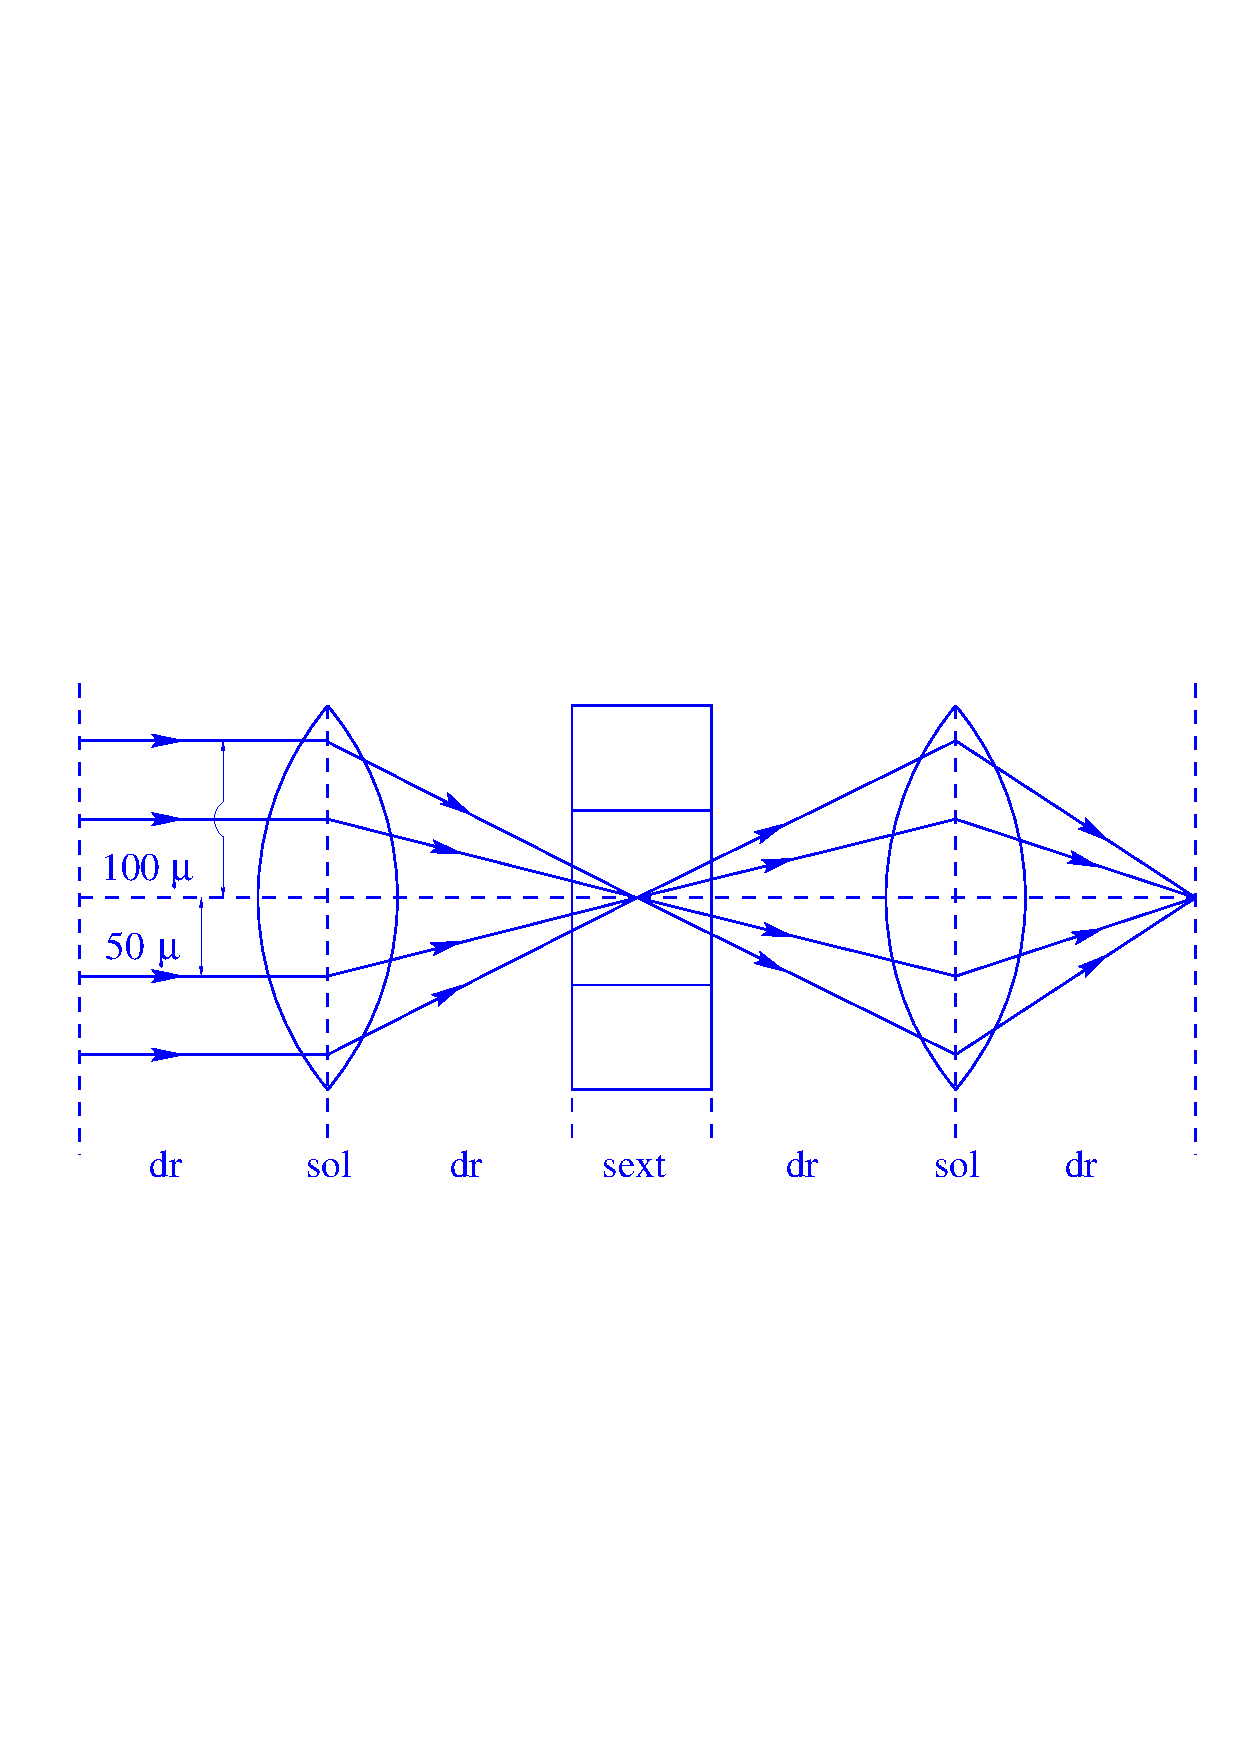
\includegraphics[height=2.5in]{fig10_4a}
  \caption{A simple spot-forming system consisting of two solenoids and
suitably chosen drifts.}
\end{figure}

\subsection{Fitting Solenoid and Sextupole Strengths}
\label{fitsole}
The \Mary run of Exhibit 10.4.1 illustrates how the two solenoid
strengths are fit to achieve a spot-forming system with an intermediate
beam crossover.  This fitting is simplified by setting IOPT=1 for each
solenoid so that the paraxial rotation parts of their respective maps are
artificially removed.  See section 6.23.  In this way one does not have to
worry about complications caused by coupling of the $x$ and $y$ plane
motions.  Once fitting of solenoid strengths has been achieved, IOPT for
each solenoid is reset to IOPT=0 by use of a {\em rset} command.  See
section 9.18.\index{fit}

After the solenoid strengths have been fit, rays are traced through the
system (with the sextupole off) to evaluate the effect of aberrations.
Similar to the case of figure 2.2.1 of section 2.2, the incoming rays lie
on two cylinders parallel to the optic axis.  In this case the cylinders
have radii of 50 and 100 $\times 10^{-6}$ meters, respectively.  See
figure 10.4.1.  The result of this ray trace is shown in figure 10.4.1.1.  While the radii of the incoming cylinders have a ratio of 2 to 1, the
ratio of the two final circles shown in figure 10.4.1.1 is 8 to 1.  This is
what is to be expected from third-order geometrical aberrations since
$2^3 = 8$.


\begin{figure}[htbp]
\setcounter{figure}{0}
  \centering
  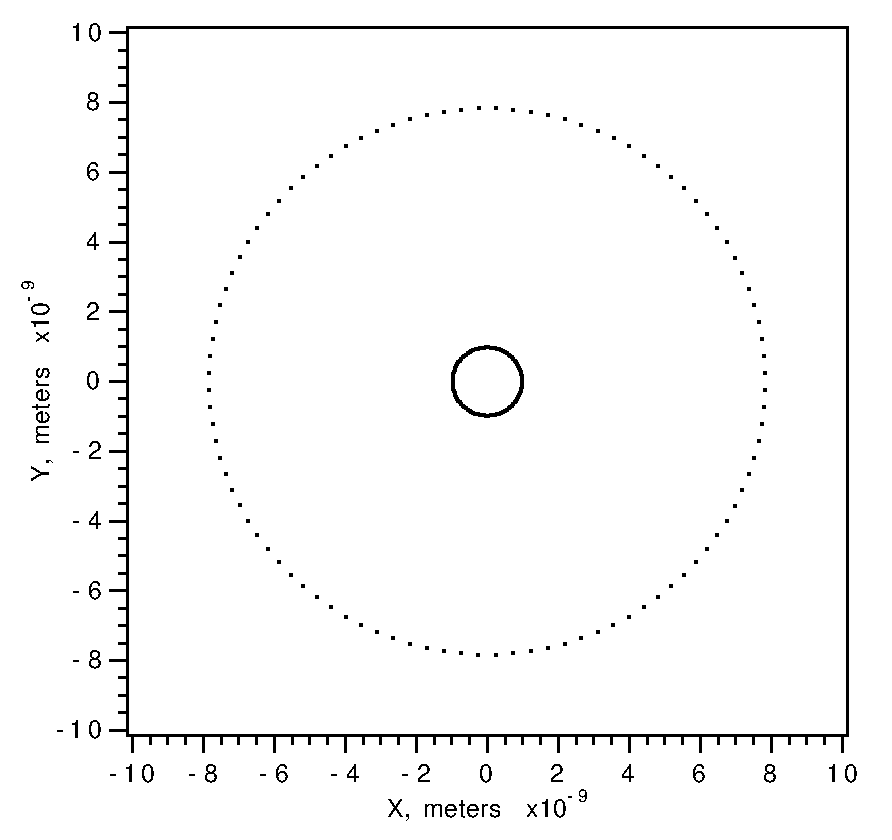
\includegraphics[height=2.5in]{fig10_4b}
  \caption{Final focal spot patterns produced by the simple (uncorrected)
Solenoid Spot-Forming System of figure 10.4.1.}
\end{figure}

Note that, for this and later parts of the run, the solenoid maps (whose
computation requires numerical integration) are stored as the lumps {\em
llens1} and {\em llens2} so that they do not have to be continually
recomputed.  See section 5.9.

Subsequently the sextupole corrector strength is set to achieve the
condition
\[
f(140) = f(149) = f(195) = 0
\]
in order to remove the aberrations detrimental to a spot-forming system.
Rays are then traced through this system using the total transfer map to
verify that correction has indeed occurred.  The results of this ray
trace are not shown, but are similar to those of figure 10.3.1.1: \ up to
fitting and roundoff errors, all rays are now brought to a point focus.
Finally, to estimate the effect of fourth and yet higher-order
aberrations not computed by \Mary 3.0 for the total transfer map, rays
are traced element-by-element using the loop {\em onebyone} and the
command circ18.  The results of this ray trace are shown in figure
10.4.1.2.  Comparison of figures 10.4.1.1 and 10.4.1.2 shows that the spot size
has shrunk by about an order of magnitude as a result of sextupole
correction.

\begin{figure}[htbp]
  \centering
  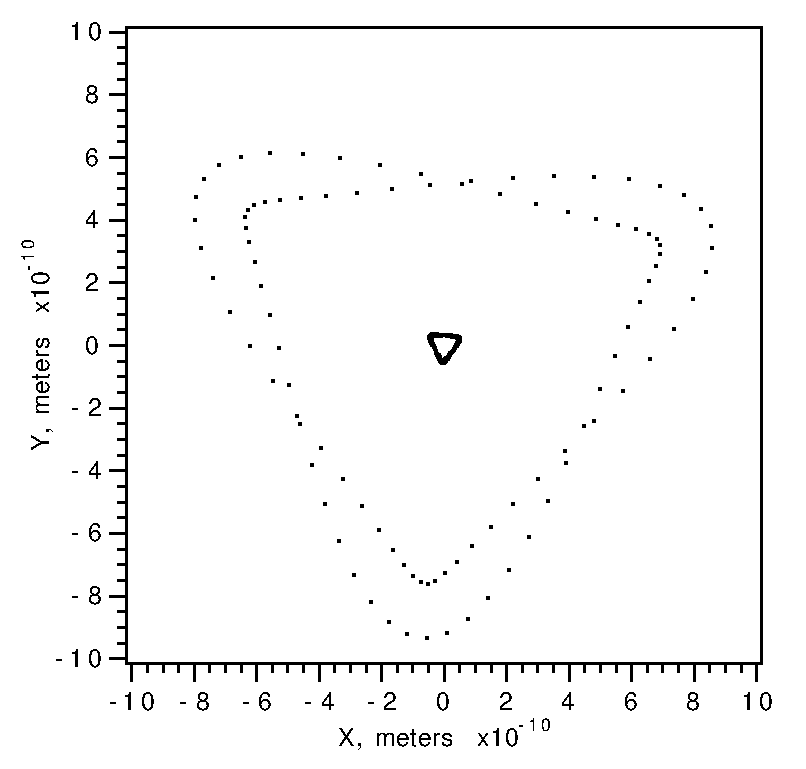
\includegraphics[width=2.65in]{fig10_4c}
  \caption{Estimated final focal spot patterns for sextupole-corrected
system.  Third order element-by-element calculation.}
\end{figure}

Exhibits 10.4.1a and 10.4.1b show the contents of the external instruction
files associated with the commands {\em aim1} and {\em vary1} that are
used to fit the strength for the solenoid {\em sol1} in the line {\em
sect1f}.  A beam crossover is achieved by requiring the condition R(1,1)
= 0 for the map associated with the line {\em sect1f}.  Exhibits
10.4.1c and 10.4.1d show the instruction files for the commands {\em
aim2} and {\em vary2} that are used to fit the strength for the solenoid
{\em sol2} in the line {\em sect2f}.  Note that imaging for the map
associated with {\em sect2f} is achieved by requiring the condition
R(1,2)=0 for this map.  Exhibit 10.4.1e shows the instruction file for
the reset command {\em rset}.\index{reset menu entries}  As described earlier, it is invoked after
the fitting of solenoid strengths is complete.  Next, Exhibits 10.4.1f
and 10.4.1g show the instruction files for the commands {\em aim3} and
{\em vary3} that are used to set the strength of the sextupole corrector.
Note that all the instructions provided by all these files could also
have been entered interactively, if desired.  Finally, Exhibit 10.4.1h
show the \Mary run itself along with explanatory remarks.

\newpage
\begin{footnotesize}
\begin{verbatim}
Exhibit 10.4.1a
Contents of file 021 that provides instructions for the command aim1:

 1    r(1,1) =      0.000000000E+00
 #


Exhibit 10.4.1b
Contents of file 022 that provides instructions for the command vary1:

 par1    4
  #


Exhibit 10.4.1c
Contents of file 023 that provides instructions for the command aim2:

 1    r(1,2) =      0.000000000E+00
 #


Exhibit 10.4.1d
Contents of file 024 that provides instructions for the command vary2:

 par2     4
  #


Exhibit 10.4.1e
Contents of file 027 that provides instructions for the command rset:

par1 6 par2 6
0
0
#


Exhibit 10.4.1f
Contents of file 025 that provides instructions for the command aim3:

 1    f(140) =      0.000000000E+00
 #


Exhibit 10.4.1g
Contents of file 026 that provides instructions for the command vary3:

 sex        2
  #


Exhibit 10.4.1h
***MARYLIE 3.0***
Prerelease Development Version 8/21/98
Copyright 1987 Alex J. Dragt
All rights reserved

Data input complete; going into #labor.
#comment
 Exhibit 10.4.1.
 This is a MARYLIE run for a sextupole corrected Solenoidal Spot-Forming
 System. The system consists of two solenoids, a sextupole, and suitably
 chosen drifts.  The beam parameters are those for 200 KeV electrons.

 This run does 8 things:

  a) The strength of the first solenoid is fit to produce a
     crossover (starting with parallel incoming rays) at the
     center of the location where the sextupole corrector is
     to be placed.  For simplicity, this fitting is carried
     out with the rotation part of the first solenoid map
     removed, and is equivalent to demanding that

     r(1,1)=0

     for the map corresponding to the line sect1f.

  b) The strength of the second solenoid is fit to image the
     crossover at a distance of .5 meter after the second
     solenoid. For simplicity, this fitting is carried
     out with the rotation part of the second solenoid map
     also removed, and is equivalent to demanding that

     r(1,2)=0


     for the map corresponding to the line sect2f.

  c) After the strengths of the two solenoids have been set,
     the map for the combined system (sect1f sect2f) is
     computed to make sure that it is spot forming as it
     should be, i.e. it should satisfy

     r(1,1)=0.


  d) As indicated, for ease of fitting the operations above
     were carried out with the rotation parts of the solenoidal
     maps removed.  After solenoidal fitting is complete, the
     6'th parameters in the parameter sets par1 and par2 are
     reset to IOPT=0 so that in subsequent use the full transfer
     maps for the solenoids will be computed.

  e) The full transfer map is computed for the sextupole corrected
     spot-forming system with the sextupole turned off (replaced
     by an equivalent drift).  A ray trace is carried out using
     this map to show the detrimental effect of third-order
     spherical aberrations described by the generators

       f(140) = f(04 00 00) = -33.7677,
       f(149) = f(02 02 00) = -67.5354, and
       f(195) = f(00 04 00) = -33.7677.

     See the results below of printing out the generators for
     the full transfer map.  Note that, due to the rotational
     symmetry of solenoids, the generators appear in the
     combination

       (Px**2 + Py**2)**2.

     That is, there are the relations

       f(195) = f(140),
       f(149) = 2f(140).

  f) The strength of the sextupole corrector corrector is fit
     to "zero out" the detrimental aberration generators.
     This is done by requiring that

       f(140) = 0.

     In so doing, the remaining aberration generators, f(149)
     and f(195),  are then also zeroed out automatically as
     a result of symmetry.

  g) A ray trace is carried out using the map for the sextupole
     corrected system to indicate that the spot size has indeed
     diminished as a result of properly powering the corrector.

  h) An element by element ray trace is carried out to estimate
     the effect of residual fourth and higher order aberrations.

#beam
 1.649033824222788E-003
 0.391390152459380
  1.00000000000000
  1.00000000000000
#menu
 fileout  pmif
   1.00000000000000       12.0000000000000       3.00000000000000
 sol1     sol
  0.000000000000000E+00  0.200000000000000       200.000000000000
  0.000000000000000E+00   1.00000000000000      0.000000000000000E+00
 sol2     sol
  0.000000000000000E+00  0.200000000000000       200.000000000000
  0.000000000000000E+00   1.00000000000000      0.000000000000000E+00
 par1     ps1
  5.000000000000000E-02  0.100000000000000      1.000000000000000E-02
  2.000000000000000E-02   3.00000000000000       1.00000000000000
 par2     ps1
  5.000000000000000E-02  0.100000000000000      1.000000000000000E-02
  2.000000000000000E-02   3.00000000000000       1.00000000000000
 dr1      drft
  0.000000000000000E+00
 dr2      drft
  0.100000000000000
 dr3      drft
  0.500000000000000
 dr4      drft
  0.500000000000000
 nosex    drft
  0.200000000000000
 nosex/2  drft
  0.100000000000000
 sex      sext
  0.200000000000000       100.000000000000
 mapout   ptm
   3.00000000000000       3.00000000000000      0.000000000000000E+00
  0.000000000000000E+00   1.00000000000000
 matout   ptm
   3.00000000000000      0.000000000000000E+00  0.000000000000000E+00
  0.000000000000000E+00   1.00000000000000
 bip      bip
   20.0000000000000
 tip      tip
  0.000000000000000E+00
 aim1     aim
   1.00000000000000       21.0000000000000      0.000000000000000E+00
  0.000000000000000E+00   1.00000000000000       1.00000000000000
 aim2     aim
   1.00000000000000       23.0000000000000      0.000000000000000E+00
  0.000000000000000E+00   1.00000000000000       1.00000000000000
 aim3     aim
   1.00000000000000       25.0000000000000      0.000000000000000E+00
  0.000000000000000E+00   1.00000000000000       1.00000000000000
 vary1    vary
   1.00000000000000       22.0000000000000      0.000000000000000E+00
  0.000000000000000E+00   1.00000000000000       1.00000000000000
 vary2    vary
   1.00000000000000       24.0000000000000      0.000000000000000E+00
  0.000000000000000E+00   1.00000000000000       1.00000000000000
 vary3    vary
   1.00000000000000       26.0000000000000      0.000000000000000E+00
  0.000000000000000E+00   1.00000000000000       1.00000000000000
 rset     rset
   1.00000000000000       27.0000000000000      0.000000000000000E+00
  0.000000000000000E+00   1.00000000000000
 fit      fit
   1.00000000000000      0.000000000000000E+00  1.000000000000000E-10
  1.000000000000000E-03   1.00000000000000       1.00000000000000
 clear    iden
 raysin   rt
   13.0000000000000       14.0000000000000      -1.00000000000000
  0.000000000000000E+00  0.000000000000000E+00  0.000000000000000E+00
 trace14  rt
  0.000000000000000E+00   14.0000000000000       4.00000000000000
  0.000000000000000E+00   1.00000000000000      0.000000000000000E+00
 trace16  rt
  0.000000000000000E+00   16.0000000000000       6.00000000000000
  0.000000000000000E+00   1.00000000000000      0.000000000000000E+00
 circ18   circ
  0.000000000000000E+00   18.0000000000000       5.00000000000000
   1.00000000000000       1.00000000000000       3.00000000000000
 end      end
#lines
 lens1
     1*par1        1*sol1
 lens2
     1*par2        1*sol1
 sect1
     1*dr1         1*llens1      1*dr2
 sect2
     1*dr3         1*llens2      1*dr4
 sect1f
     1*dr1         1*lens1       1*dr2         1*nosex/2
 sect2f
     1*nosex/2     1*dr3         1*lens2       1*dr4
 spot
     1*sect1       1*nosex       1*sect2
 cspot
     1*sect1       1*sex         1*sect2
#lumps
 llens1
     1*lens1
 llens2
     1*lens2
#loops
 onebyone
     1*cspot
#labor
    1*fileout
    1*sect1f
    1*aim1
    1*vary1
    1*bip
    1*clear
    1*sect1f
    1*fit
    1*tip
    1*matout
    1*clear
    1*sect2f
    1*aim2
    1*vary2
    1*bip
    1*clear
    1*sect2f
    1*fit
    1*tip
    1*matout
    1*clear
    1*sect1f
    1*sect2f
    1*matout
    1*rset
    1*clear
    1*spot
    1*mapout
    1*raysin
    1*trace14
    1*clear
    1*cspot
    1*mapout
    1*aim3
    1*vary3
    1*bip
    1*clear
    1*cspot
    1*fit
    1*tip
    1*mapout
    1*raysin
    1*trace16
    1*clear
    1*raysin
    1*onebyone
    1*circ18
    1*end

 zi=  0.000000000000000E+000 zf=  0.200000000000000
 ns=         200
 di=  5.000000000000000E-002 length=  0.100000000000000
 cl=  1.000000000000000E-002 B=  2.000000000000000E-002
 iopt=           1

 symplectic violation =   1.554312234475219E-015

**********************
* Response to aim1:  *
**********************

accept  1:      r(1,1)

 Aims selected :
No.     item      present value
----------------------------------
 1    r(1,1) =      5.358248605E-02

**********************
* Response to vary1: *
**********************

No.  1 is par1     ps1     .  Parameter 4 out of 6 selected.
     par1(4) =  2.00000000000000E-02

  Variable #menu elements selected:
No.  Element    Type     Parameter   Present value
-----------------------------------------------------------
 1    par1       ps1          4      2.00000000000000E-02

****************************
* First fitting procedure: *
****************************

 zi=  0.000000000000000E+000 zf=  0.200000000000000
 ns=         200
 di=  5.000000000000000E-002 length=  0.100000000000000
 cl=  1.000000000000000E-002 B=  2.000000000000000E-002
 iopt=           1

 symplectic violation =   1.554312234475219E-015


 target           1 =  0.000000000000000E+000
Iter   1 Error= 5.3582E-02,  Step= 2.0000E-05,  SubErr= 5.3582E-02 @cut=    1
-------------------------------------------------------

 zi=  0.000000000000000E+000 zf=  0.200000000000000
 ns=         200
 di=  5.000000000000000E-002 length=  0.100000000000000
 cl=  1.000000000000000E-002 B=  2.002000000000000E-002
 iopt=
        1
 symplectic violation =   8.881784197001252E-016

********************************************
* ETC. ETC. ETC.                           *
********************************************

 zi=  0.000000000000000E+000 zf=  0.200000000000000
 ns=         200
 di=  5.000000000000000E-002 length=  0.100000000000000
 cl=  1.000000000000000E-002 B=  2.058806040588981E-002
 iopt=           1

 symplectic violation =   3.774758283725532E-015

Quit on iteration   6 for reason 1: Converged: error < tolerance
Final values with reach =   1 are:

 Aims selected :
No.     item        present value        target value
----------------------------------------------------
 1    r(1,1) =     -8.881784197E-16     0.000000000E+00

 New values for parameters:
No.  Element    Type   Parameter   Present value         IDV  Slope
-----------------------------------------------------------------------
 1   par1       ps1        4      2.05880604058898E-02

 Maximum error is     8.881784E-16
 Maximum allowed was  1.000000E-10

*****************************************************************************
* Matrix part of map for sect1f showing that fitting has been accomplished: *
*****************************************************************************

matrix for map is :

-8.88178E-16  3.01323E-01  0.00000E+00  0.00000E+00  0.00000E+00  0.00000E+00
-3.31870E+00  6.63740E-01  0.00000E+00  0.00000E+00  0.00000E+00  0.00000E+00
 0.00000E+00  0.00000E+00 -8.88178E-16  3.01323E-01  0.00000E+00  0.00000E+00
 0.00000E+00  0.00000E+00 -3.31870E+00  6.63740E-01  0.00000E+00  0.00000E+00
 0.00000E+00  0.00000E+00  0.00000E+00  0.00000E+00  1.00000E+00  4.27366E-01
 0.00000E+00  0.00000E+00  0.00000E+00  0.00000E+00  0.00000E+00  1.00000E+00

 zi=  0.000000000000000E+000 zf=  0.200000000000000
 ns=         200
 di=  5.000000000000000E-002 length=  0.100000000000000
 cl=  1.000000000000000E-002 B=  2.000000000000000E-002
 iopt=           1

 symplectic violation =   1.554312234475219E-015

**********************
* Response to aim2:  *
**********************

accept  1:      r(1,2)

 Aims selected :
No.     item      present value
----------------------------------
 1    r(1,2) =     -2.210611452E-02

**********************
* Response to vary2: *
**********************

No.  1 is par2     ps1     .  Parameter 4 out of 6 selected.
     par2(4) =  2.00000000000000E-02

  Variable #menu elements selected:
No.  Element    Type     Parameter   Present value
-----------------------------------------------------------
 1    par2       ps1          4      2.00000000000000E-02

*****************************
* Second fitting procedure: *
*****************************

 zi=  0.000000000000000E+000 zf=  0.200000000000000
 ns=         200
 di=  5.000000000000000E-002 length=  0.100000000000000
 cl=  1.000000000000000E-002 B=  2.000000000000000E-002
 iopt=           1

 symplectic violation =   1.554312234475219E-015

 target           1 =  0.000000000000000E+000
Iter   1 Error= 2.2106E-02,  Step= 2.0000E-05,  SubErr= 2.2106E-02 @cut=    1
-------------------------------------------------------

 zi=  0.000000000000000E+000 zf=  0.200000000000000
 ns=         200
 di=  5.000000000000000E-002 length=  0.100000000000000
 cl=  1.000000000000000E-002 B=  2.002000000000000E-002
 iopt=           1

 symplectic violation =   8.881784197001252E-016

********************************************
* ETC. ETC. ETC.                           *
********************************************

 zi=  0.000000000000000E+000 zf=  0.200000000000000
 ns=         200
 di=  5.000000000000000E-002 length=  0.100000000000000
 cl=  1.000000000000000E-002 B=  1.982359647711195E-002
 iopt=           1

 symplectic violation =   1.776356839400250E-015
Quit on iteration   5 for reason 1: Converged: error < tolerance
Final values with reach =   1 are:

 Aims selected :
No.     item        present value        target value
----------------------------------------------------
 1    r(1,2) =     -4.293787548E-12     0.000000000E+00

 New values for parameters:
No.  Element    Type   Parameter   Present value         IDV  Slope
-----------------------------------------------------------------------
 1   par2       ps1        4      1.98235964771120E-02

 Maximum error is     4.293788E-12
 Maximum allowed was  1.000000E-10

*****************************************************************************
* Matrix part of map for sect2f showing that fitting has been accomplished: *
*****************************************************************************

matrix for map is :

-8.57392E-01 -4.29379E-12  0.00000E+00  0.00000E+00  0.00000E+00  0.00000E+00
-3.08935E+00 -1.16633E+00  0.00000E+00  0.00000E+00  0.00000E+00  0.00000E+00
 0.00000E+00  0.00000E+00 -8.57392E-01 -4.29379E-12  0.00000E+00  0.00000E+00
 0.00000E+00  0.00000E+00 -3.08935E+00 -1.16633E+00  0.00000E+00  0.00000E+00
 0.00000E+00  0.00000E+00  0.00000E+00  0.00000E+00  1.00000E+00  1.38894E+00
 0.00000E+00  0.00000E+00  0.00000E+00  0.00000E+00  0.00000E+00  1.00000E+00

 zi=  0.000000000000000E+000 zf=  0.200000000000000
 ns=         200
 di=  5.000000000000000E-002 length=  0.100000000000000
 cl=  1.000000000000000E-002 B=  2.058806040588981E-002
 iopt=           1

 symplectic violation =   3.774758283725532E-015

 zi=  0.000000000000000E+000 zf=  0.200000000000000
 ns=         200
 di=  5.000000000000000E-002 length=  0.100000000000000
 cl=  1.000000000000000E-002 B=  1.982359647711195E-002
 iopt=           1

 symplectic violation =   1.776356839400250E-015

*****************************************************************************
* Matrix part of map for sect1f sect2f showing that is indeed spot forming; *
*****************************************************************************

matrix for map is :

 1.42508E-11 -2.58352E-01  0.00000E+00  0.00000E+00  0.00000E+00  0.00000E+00
 3.87069E+00 -1.70503E+00  0.00000E+00  0.00000E+00  0.00000E+00  0.00000E+00
 0.00000E+00  0.00000E+00  1.42508E-11 -2.58352E-01  0.00000E+00  0.00000E+00
 0.00000E+00  0.00000E+00  3.87069E+00 -1.70503E+00  0.00000E+00  0.00000E+00
 0.00000E+00  0.00000E+00  0.00000E+00  0.00000E+00  1.00000E+00  1.81630E+00
 0.00000E+00  0.00000E+00  0.00000E+00  0.00000E+00  0.00000E+00  1.00000E+00

*********************
* Response to rset: *
*********************

MARYLIE #menu entries available to be varied:
-----------------------------------------------------------------------
aim1     circ18   dr3      fit      nosex/2  rset     tip      vary2
aim2     clear    dr4      mapout   par1     sex      trace14  vary3
aim3     dr1      end      matout   par2     sol1     trace16
bip      dr2      fileout  nosex    raysin   sol2     vary1

To RESET #menu items, enter name and (optional) parameter index.
Type * to relist, or a # sign when finished.

The following  2 #menu item(s) have been reset:
No.   Item       Type     Parameter   New value
-----------------------------------------------------------
 1    par1       ps1          6      0.00000000000000E+00
 2    par2       ps1          6      0.00000000000000E+00

 zi=  0.000000000000000E+000 zf=  0.200000000000000
 ns=         200
 di=  5.000000000000000E-002 length=  0.100000000000000
 cl=  1.000000000000000E-002 B=  2.058806040588981E-002
 iopt=           0

 symplectic violation =   1.457667320181599E-01

lump llens1   constructed and stored.( 1)

 zi=  0.000000000000000E+000 zf=  0.200000000000000
 ns=         200
 di=  5.000000000000000E-002 length=  0.100000000000000
 cl=  1.000000000000000E-002 B=  1.982359647711195E-002
 iopt=           0

 symplectic violation =   1.325245468919434E-012

lump llens2   constructed and stored.( 2)

**********************************************************
* Map for spot forming system with sextupole turned off: *
**********************************************************

matrix for map is :

 3.92752E-12 -8.74925E-02  1.36455E-11 -2.43086E-01  0.00000E+00  0.00000E+00
 1.31084E+00 -5.77420E-01  3.64197E+00 -1.60428E+00  0.00000E+00  0.00000E+00
-1.36451E-11  2.43086E-01  3.92752E-12 -8.74925E-02  0.00000E+00  0.00000E+00
-3.64197E+00  1.60428E+00  1.31084E+00 -5.77420E-01  0.00000E+00  0.00000E+00
 0.00000E+00  0.00000E+00  0.00000E+00  0.00000E+00  1.00000E+00  1.81630E+00
 0.00000E+00  0.00000E+00  0.00000E+00  0.00000E+00  0.00000E+00  1.00000E+00

nonzero elements in generating polynomial are :

 f( 33)=f( 20 00 01 )= -19.354345343837
 f( 38)=f( 11 00 01 )=  8.5317869933313
 f( 42)=f( 10 10 01 )= 1.77635683940025E-15
 f( 45)=f( 10 01 01 )=  1.7622352560429
 f( 53)=f( 02 00 01 )= -1.8284384427366
 f( 57)=f( 01 10 01 )= -1.7622352560429
 f( 60)=f( 01 01 01 )= 3.19189119579733E-16
 f( 67)=f( 00 20 01 )= -19.354345343837
 f( 70)=f( 00 11 01 )=  8.5317869933313
 f( 76)=f( 00 02 01 )= -1.8284384427366
 f( 83)=f( 00 00 03 )= -1.3061027823091
 f( 84)=f( 40 00 00 )= -5368.1678868663
 f( 85)=f( 31 00 00 )=  3124.3698789490
 f( 86)=f( 30 10 00 )= 1.72228897810101E-11
 f( 87)=f( 30 01 00 )=  75.164310605427
 f( 90)=f( 22 00 00 )= -1010.3164650898
 f( 91)=f( 21 10 00 )= -75.164310605444
 f( 92)=f( 21 01 00 )= -30.445062048227
 f( 95)=f( 20 20 00 )= -10736.335773733
 f( 96)=f( 20 11 00 )=  3124.3698789490
 f( 99)=f( 20 02 00 )= -341.27794387998
 f(104)=f( 20 00 02 )= -88.367907544732
 f(105)=f( 13 00 00 )=  255.03547488004
 f(106)=f( 12 10 00 )=  30.445062048233
 f(107)=f( 12 01 00 )=  5.5596519517141
 f(110)=f( 11 20 00 )=  3124.3698789490
 f(111)=f( 11 11 00 )= -1338.0770424196
 f(114)=f( 11 02 00 )=  255.03547488004
 f(119)=f( 11 00 02 )=  62.904770756084
 f(120)=f( 10 30 00 )= 7.26174675946822E-12
 f(121)=f( 10 21 00 )=  75.164310605425
 f(124)=f( 10 12 00 )= -30.445062048228
 f(129)=f( 10 10 02 )= 5.49862591908003E-14
 f(130)=f( 10 03 00 )=  5.5596519517147
 f(135)=f( 10 01 02 )=  3.1890117279099
 f(140)=f( 04 00 00 )= -33.767743155594
 f(141)=f( 03 10 00 )= -5.5596519517151
 f(142)=f( 03 01 00 )= 3.83495318834193E-14
 f(145)=f( 02 20 00 )= -341.27794387998
 f(146)=f( 02 11 00 )=  255.03547488004
 f(149)=f( 02 02 00 )= -67.535486311188
 f(154)=f( 02 00 02 )= -10.294678284563
 f(155)=f( 01 30 00 )= -75.164310605433
 f(156)=f( 01 21 00 )=  30.445062048232
 f(159)=f( 01 12 00 )= -5.5596519517156
 f(164)=f( 01 10 02 )= -3.1890117279099
 f(165)=f( 01 03 00 )= 1.42049566553837E-13
 f(170)=f( 01 01 02 )= 9.90874049477952E-15
 f(175)=f( 00 40 00 )= -5368.1678868663
 f(176)=f( 00 31 00 )=  3124.3698789490
 f(179)=f( 00 22 00 )= -1010.3164650898
 f(184)=f( 00 20 02 )= -88.367907544732
 f(185)=f( 00 13 00 )=  255.03547488004
 f(190)=f( 00 11 02 )=  62.904770756084
 f(195)=f( 00 04 00 )= -33.767743155594
 f(200)=f( 00 02 02 )= -10.294678284563
 f(209)=f( 00 00 04 )= -2.1210054140684

****************************************************************
* Ray trace for spot forming system with sextupole turned off: *
****************************************************************

  200 ray(s) read in from file  13

*****************************************************************
* Map for spot forming system with sextupole partially powered: *
*****************************************************************

matrix for map is :

 3.92752E-12 -8.74925E-02  1.36455E-11 -2.43086E-01  0.00000E+00  0.00000E+00
 1.31084E+00 -5.77420E-01  3.64197E+00 -1.60428E+00  0.00000E+00  0.00000E+00
-1.36451E-11  2.43086E-01  3.92752E-12 -8.74925E-02  0.00000E+00  0.00000E+00
-3.64197E+00  1.60428E+00  1.31084E+00 -5.77420E-01  0.00000E+00  0.00000E+00
 0.00000E+00  0.00000E+00  0.00000E+00  0.00000E+00  1.00000E+00  1.81630E+00
 0.00000E+00  0.00000E+00  0.00000E+00  0.00000E+00  0.00000E+00  1.00000E+00

nonzero elements in generating polynomial are :

 f( 28)=f( 30 00 00 )= -1580.8951974218
 f( 29)=f( 21 00 00 )=  57.529446412786
 f( 30)=f( 20 10 00 )= -20039.007779464
 f( 31)=f( 20 01 00 )=  243.07599601673
 f( 33)=f( 20 00 01 )= -19.354345343837
 f( 34)=f( 12 00 00 )= -7.9831068587096
 f( 35)=f( 11 10 00 )=  486.15199203346
 f( 36)=f( 11 01 00 )= -67.461161965202
 f( 38)=f( 11 00 01 )=  8.5317869933313
 f( 39)=f( 10 20 00 )=  4742.6855922654
 f( 40)=f( 10 11 00 )= -115.05889282557
 f( 42)=f( 10 10 01 )= 1.77635683940025E-15
 f( 43)=f( 10 02 00 )=  7.9831068587118
 f( 45)=f( 10 01 01 )=  1.7622352560429
 f( 49)=f( 03 00 00 )= 3.52997631125618E-11
 f( 50)=f( 02 10 00 )= -33.730580982600
 f( 51)=f( 02 01 00 )= 3.67890606867149E-10
 f( 53)=f( 02 00 01 )= -1.8284384427366
 f( 54)=f( 01 20 00 )= -57.529446412787
 f( 55)=f( 01 11 00 )=  15.966213717424
 f( 57)=f( 01 10 01 )= -1.7622352560429
 f( 58)=f( 01 02 00 )=-1.07888808997814E-10
 f( 60)=f( 01 01 01 )= 3.19189119579733E-16
 f( 64)=f( 00 30 00 )=  6679.6692598213
 f( 65)=f( 00 21 00 )= -243.07599601673
 f( 67)=f( 00 20 01 )= -19.354345343837
 f( 68)=f( 00 12 00 )=  33.730580982599
 f( 70)=f( 00 11 01 )=  8.5317869933313
 f( 74)=f( 00 03 00 )=-1.22327037388459E-10
 f( 76)=f( 00 02 01 )= -1.8284384427366
 f( 83)=f( 00 00 03 )= -1.3061027823091
 f( 84)=f( 40 00 00 )=  4534434.9355423
 f( 85)=f( 31 00 00 )= -417.18711658195
 f( 86)=f( 30 10 00 )=-1.58325412780158E-08
 f( 87)=f( 30 01 00 )=  75.164314169984
 f( 89)=f( 30 00 01 )= -4135.3649240237
 f( 90)=f( 22 00 00 )=  464.02211364079
 f( 91)=f( 21 10 00 )= -75.164314147981
 f( 92)=f( 21 01 00 )= -30.445062007087
 f( 94)=f( 21 00 01 )=  6096.0173475002
 f( 95)=f( 20 20 00 )=  9068869.8710847
 f( 96)=f( 20 11 00 )= -417.18711659685
 f( 98)=f( 20 10 01 )= -56889.773039091
 f( 99)=f( 20 02 00 )= -39075.431813770
 f(101)=f( 20 01 01 )=  25811.399464434
 f(104)=f( 20 00 02 )= -88.367907544732
 f(105)=f( 13 00 00 )= -17.747784419917
 f(106)=f( 12 10 00 )=  30.445061995271
 f(107)=f( 12 01 00 )=  5.5596519387338
 f(109)=f( 12 00 01 )= -155.63630755806
 f(110)=f( 11 20 00 )= -417.18711658567
 f(111)=f( 11 11 00 )=  79078.907854842
 f(113)=f( 11 10 01 )=  51622.798928869
 f(114)=f( 11 02 00 )= -17.747784425039
 f(116)=f( 11 01 01 )= -1330.2545443094
 f(119)=f( 11 00 02 )=  62.904770756084
 f(120)=f( 10 30 00 )= 7.45056638606911E-09
 f(121)=f( 10 21 00 )=  75.164314153104
 f(123)=f( 10 20 01 )=  12406.094772071
 f(124)=f( 10 12 00 )= -30.445061992942
 f(126)=f( 10 11 01 )= -12192.034695000
 f(129)=f( 10 10 02 )= 5.49862591908003E-14
 f(130)=f( 10 03 00 )=  5.5596519354159
 f(132)=f( 10 02 01 )=  155.63630755804
 f(135)=f( 10 01 02 )=  3.1890117279099
 f(140)=f( 04 00 00 )= -14.841279885615
 f(141)=f( 03 10 00 )= -5.5596519367838
 f(142)=f( 03 01 00 )= 9.82282501865717E-11
 f(144)=f( 03 00 01 )=  9.7710840812635
 f(145)=f( 02 20 00 )= -39075.431813776
 f(146)=f( 02 11 00 )= -17.747784422245
 f(148)=f( 02 10 01 )= -665.12727215468
 f(149)=f( 02 02 00 )= -29.682559770183
 f(151)=f( 02 01 01 )=  123.85566749550
 f(154)=f( 02 00 02 )= -10.294678284563
 f(155)=f( 01 30 00 )= -75.164314166142
  f(156)=f( 01 21 00 )=  30.445062003885
 f(158)=f( 01 20 01 )= -6096.0173475002
 f(159)=f( 01 12 00 )= -5.5596519411203
 f(161)=f( 01 11 01 )=  311.27261511610
 f(164)=f( 01 10 02 )= -3.1890117279099
 f(165)=f( 01 03 00 )= 1.28056848111568E-09
 f(167)=f( 01 02 01 )= -29.313252243794
 f(170)=f( 01 01 02 )= 9.90874049477952E-15
 f(175)=f( 00 40 00 )=  4534434.9355423
 f(176)=f( 00 31 00 )= -417.18711657636
 f(178)=f( 00 30 01 )=  18963.257679697
 f(179)=f( 00 22 00 )=  464.02211363707
 f(181)=f( 00 21 01 )= -25811.399464434
 f(184)=f( 00 20 02 )= -88.367907544732
 f(185)=f( 00 13 00 )= -17.747784420382
 f(187)=f( 00 12 01 )=  665.12727215469
 f(190)=f( 00 11 02 )=  62.904770756084
 f(195)=f( 00 04 00 )= -14.841279885324
 f(197)=f( 00 03 01 )= -41.285222498500
 f(200)=f( 00 02 02 )= -10.294678284563
 f(209)=f( 00 00 04 )= -2.1210054140684

*********************
* Response to aim3: *
*********************

accept  1:      f(140)

 Aims selected :
No.     item      present value
----------------------------------
 1    f(140) =      -14.8412799

**********************
* Response to vary3: *
**********************

No.  1 is sex      sext    .  Parameter 2 out of 2 selected.
      sex(2) =   100.00000000000

  Variable #menu elements selected:
No.  Element    Type     Parameter   Present value
-----------------------------------------------------------
 1    sex        sext         2       100.00000000000

*****************************************
* Beginning of third fitting procedure: *
*****************************************

 target           1 =  0.000000000000000E+000
Iter   1 Error= 1.4841E+01,  Step= 1.0000E-01,  SubErr= 1.4841E+01 @cut=    1
-------------------------------------------------------

********************************************
* ETC. ETC. ETC.                           *
********************************************

Quit on iteration   8 for reason 2: Best effort: Hit bottom at full reach
Final values with reach =   1 are:

 Aims selected :
No.     item        present value        target value
----------------------------------------------------
 1    f(140) =     -1.222360879E-09     0.000000000E+00

 New values for parameters:
No.  Element    Type   Parameter   Present value         IDV  Slope
-----------------------------------------------------------------------
 1   sex        sext       2       133.57226325988

 Maximum error is     1.222361E-09
 Maximum allowed was  1.000000E-10

**********************************************
* Map for fully fitted and corrected system: *
**********************************************

matrix for map is :

 3.92752E-12 -8.74925E-02  1.36455E-11 -2.43086E-01  0.00000E+00  0.00000E+00
 1.31084E+00 -5.77420E-01  3.64197E+00 -1.60428E+00  0.00000E+00  0.00000E+00
-1.36451E-11  2.43086E-01  3.92752E-12 -8.74925E-02  0.00000E+00  0.00000E+00
-3.64197E+00  1.60428E+00  1.31084E+00 -5.77420E-01  0.00000E+00  0.00000E+00
 0.00000E+00  0.00000E+00  0.00000E+00  0.00000E+00  1.00000E+00  1.81630E+00
 0.00000E+00  0.00000E+00  0.00000E+00  0.00000E+00  0.00000E+00  1.00000E+00

nonzero elements in generating polynomial are :

 f( 28)=f( 30 00 00 )= -2111.6374949631
 f( 29)=f( 21 00 00 )=  76.843383614438
 f( 30)=f( 20 10 00 )= -26766.556225854
 f( 31)=f( 20 01 00 )=  324.68210932105
 f( 33)=f( 20 00 01 )= -19.354345343837
 f( 34)=f( 12 00 00 )= -10.663216509634
 f( 35)=f( 11 10 00 )=  649.36421864209
 f( 36)=f( 11 01 00 )= -90.109400858331
 f( 38)=f( 11 00 01 )=  8.5317869933313
 f( 39)=f( 10 20 00 )=  6334.9124848893
 f( 40)=f( 10 11 00 )= -153.68676722888
 f( 42)=f( 10 10 01 )= 1.77635683940025E-15
 f( 43)=f( 10 02 00 )=  10.663216509637
 f( 45)=f( 10 01 01 )=  1.7622352560429
 f( 49)=f( 03 00 00 )= 4.74926764582051E-11
 f( 50)=f( 02 10 00 )= -45.054700429167
 f( 51)=f( 02 01 00 )= 4.90217644255608E-10
 f( 53)=f( 02 00 01 )= -1.8284384427366
 f( 54)=f( 01 20 00 )= -76.843383614437
 f( 55)=f( 01 11 00 )=  21.326433019271
 f( 57)=f( 01 10 01 )= -1.7622352560429
 f( 58)=f( 01 02 00 )=-1.44609657581896E-10
 f( 60)=f( 01 01 01 )= 3.19189119579733E-16
 f( 64)=f( 00 30 00 )=  8922.1854086180
 f( 65)=f( 00 21 00 )= -324.68210932103
 f( 67)=f( 00 20 01 )= -19.354345343837
 f( 68)=f( 00 12 00 )=  45.054700429161
 f( 70)=f( 00 11 01 )=  8.5317869933313
 f( 74)=f( 00 03 00 )=-1.62799551617354E-10
 f( 76)=f( 00 02 01 )= -1.8284384427366
 f( 83)=f( 00 00 03 )= -1.3061027823091
 f( 84)=f( 40 00 00 )=  8094344.0167363
 f( 85)=f( 31 00 00 )= -3194.3165697586
 f( 86)=f( 30 10 00 )= 2.98022648781426E-08
 f( 87)=f( 30 01 00 )=  75.164316937991
 f( 89)=f( 30 00 01 )= -5523.7005230738
 f( 90)=f( 22 00 00 )=  1620.1320099849
 f( 91)=f( 21 10 00 )= -75.164316997363
 f( 92)=f( 21 01 00 )= -30.445061940206
 f( 94)=f( 21 00 01 )=  8142.5883397711
 f( 95)=f( 20 20 00 )=  16188688.033473
 f( 96)=f( 20 11 00 )= -3194.3165697176
 f( 98)=f( 20 10 01 )= -75988.957411725
 f( 99)=f( 20 02 00 )= -69449.010352819
 f(101)=f( 20 01 01 )=  34476.870443694
 f(104)=f( 20 00 02 )= -88.367907544732
 f(105)=f( 13 00 00 )= -231.65212782705
 f(106)=f( 12 10 00 )=  30.445061980602
 f(107)=f( 12 01 00 )=  5.5596519154216
 f(109)=f( 12 00 01 )= -207.88693845939
 f(110)=f( 11 20 00 )= -3194.3165697195
 f(111)=f( 11 11 00 )=  142138.28472555
 f(113)=f( 11 10 01 )=  68953.740887388
 f(114)=f( 11 02 00 )= -231.65212781727
 f(116)=f( 11 01 01 )= -1776.8511019515
 f(119)=f( 11 00 02 )=  62.904770756084
 f(120)=f( 10 30 00 )=-2.98023365985500E-08
 f(121)=f( 10 21 00 )=  75.164316997363
 f(123)=f( 10 20 01 )=  16571.101569221
 f(124)=f( 10 12 00 )= -30.445061979904
 f(126)=f( 10 11 01 )= -16285.176679542
 f(129)=f( 10 10 02 )= 5.49862591908003E-14
 f(130)=f( 10 03 00 )=  5.5596519271504
 f(132)=f( 10 02 01 )=  207.88693845939
 f(135)=f( 10 01 02 )=  3.1890117279099
 f(140)=f( 04 00 00 )=-1.22236087918282E-09
 f(141)=f( 03 10 00 )= -5.5596519279799
 f(142)=f( 03 01 00 )= 1.46610828165306E-09
 f(144)=f( 03 00 01 )=  13.051458152368
 f(145)=f( 02 20 00 )= -69449.010352816
 f(146)=f( 02 11 00 )= -231.65212781914
 f(148)=f( 02 10 01 )= -888.42555097574
 f(149)=f( 02 02 00 )=-5.23868948221207E-09
 f(151)=f( 02 01 01 )=  165.43681824937
 f(154)=f( 02 00 02 )= -10.294678284563
 f(155)=f( 01 30 00 )= -75.164316935896
 f(156)=f( 01 21 00 )=  30.445061932406
 f(158)=f( 01 20 01 )= -8142.5883397711
 f(159)=f( 01 12 00 )= -5.5596519116672
 f(161)=f( 01 11 01 )=  415.77387691878
 f(164)=f( 01 10 02 )= -3.1890117279099
 f(165)=f( 01 03 00 )=-1.65891839501442E-09
 f(167)=f( 01 02 01 )= -39.154374457109
 f(170)=f( 01 01 02 )= 9.90874049477952E-15
 f(175)=f( 00 40 00 )=  8094344.0167363
 f(176)=f( 00 31 00 )= -3194.3165697567
 f(178)=f( 00 30 01 )=  25329.652470575
 f(179)=f( 00 22 00 )=  1620.1320099793
 f(181)=f( 00 21 01 )= -34476.870443694
 f(184)=f( 00 20 02 )= -88.367907544732
 f(185)=f( 00 13 00 )= -231.65212782333
 f(187)=f( 00 12 01 )=  888.42555097573
 f(190)=f( 00 11 02 )=  62.904770756084
 f(195)=f( 00 04 00 )=-2.38651409745216E-09
 f(197)=f( 00 03 01 )= -55.145606083124
 f(200)=f( 00 02 02 )= -10.294678284563
 f(209)=f( 00 00 04 )= -2.1210054140684

*****************************************
* Ray trace for fully corrected system: *
*****************************************

  200 ray(s) read in from file  13

************************************************************
* Element by element ray trace for fully corrected system: *
************************************************************

  200 ray(s) read in from file  13

circulating through onebyone :
 dr1      llens1   dr2      sex      dr3
 llens2   dr4

end of MARYLIE run
\end{verbatim}
\end{footnotesize}

\subsection{Scanning the Sextupole Strength}\index{scan}
\label{scanning}
The results of Exhibit 10.4.1h show that the third-order spherical
aberration vanishes when the sextupole corrector has the strength
S=133.57 Tesla/(meter)$^2$.  One might wonder how the spherical
aberration, as measured say by the value of f(140), varies as the
sextupole strength is varied.  Questions of this sort can be addressed by
use of the {\em scan} and {\em wsq} commands within a logical loop.  See
sections 9.14 and 8.27.  The answer to our question in this case is given
by the graph in figure 10.4.2.1.  It shows that the spherical aberration is
an even {\em quadratic} function of S that crosses zero at S = $\pm$
133.57.

Figure 10.4.2.1 was prepared by plotting the file shown in Exhibit 10.4.2a.
This file was written by the {\em wsq} command in the \Mary run shown in
the remaining parts of Exhibit 10.4.2.  In particular, Exhibits 10.4.2b
and 10.4.2c show the instruction files for the commands {\em svary} and
{\em sq} that are issued prior to entering the logical loop.  See
sections 9.6 and 8.26.  Finally, Exhibit 10.4.2d shows the \Mary run
itself.  Scanning the parameter value for the sextupole strength and
writing out the value of the parameter and the corresponding value of
f(140) on file 10 are carried out in {\em \#labor} by the commands in the
logical loop listed below:
\begin{center}
bip \\
scan \\
clear \\
cspot \\
wsq \\
tip
\end{center}

\begin{figure}[htbp]
\setcounter{figure}{0}
  \centering
  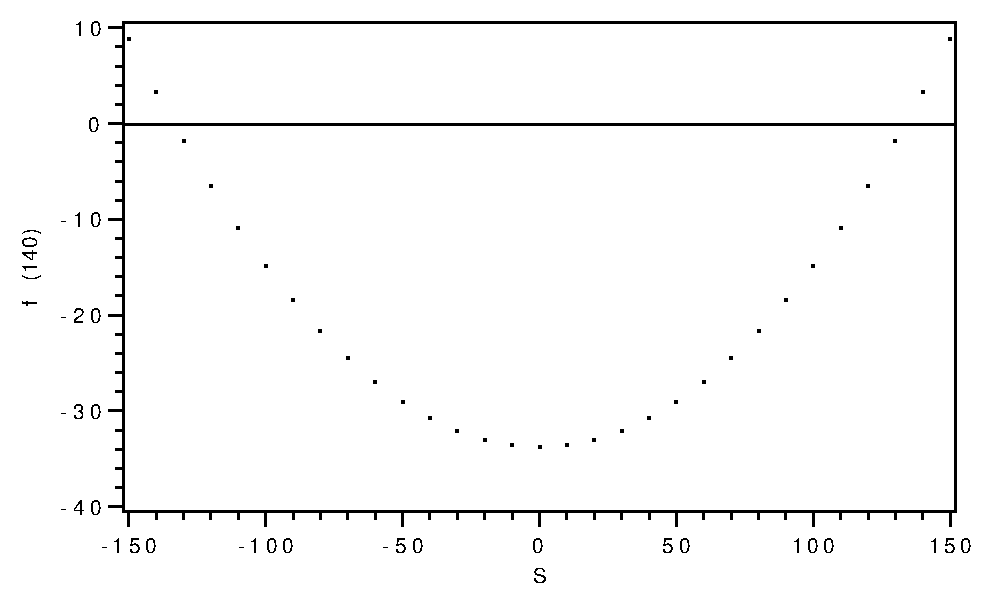
\includegraphics[height=2.5in]{fig10_4d}
  \caption{Spherical aberration of the Solenoidal Spot-Forming System as a
function of the sextupole corrector strength.}
\end{figure}

\newpage
\begin{footnotesize}
\begin{verbatim}
Exhibit 10.4.2a
Contents of file 10 resulting from use of the scan and wsq commands.
The first column is the sextupole strength S, and the second is f(140)
for the total transfer map for the Solenoidal Spot-Forming System.

-1.50000E+02  8.81680E+00
-1.40000E+02  3.32812E+00
-1.30000E+02 -1.78202E+00
-1.20000E+02 -6.51364E+00
-1.10000E+02 -1.08667E+01
-1.00000E+02 -1.48413E+01
-9.00000E+01 -1.84373E+01
-8.00000E+01 -2.16548E+01
-7.00000E+01 -2.44938E+01
-6.00000E+01 -2.69542E+01
-5.00000E+01 -2.90361E+01
-4.00000E+01 -3.07395E+01
-3.00000E+01 -3.20644E+01
-2.00000E+01 -3.30107E+01
-1.00000E+01 -3.35785E+01
 0.00000E+00 -3.37677E+01
 1.00000E+01 -3.35785E+01
 2.00000E+01 -3.30107E+01
 3.00000E+01 -3.20644E+01
 4.00000E+01 -3.07395E+01
 5.00000E+01 -2.90361E+01
 6.00000E+01 -2.69542E+01
 7.00000E+01 -2.44938E+01
 8.00000E+01 -2.16548E+01
 9.00000E+01 -1.84373E+01
 1.00000E+02 -1.48413E+01
 1.10000E+02 -1.08667E+01
 1.20000E+02 -6.51364E+00
 1.30000E+02 -1.78202E+00
 1.40000E+02  3.32812E+00
 1.50000E+02  8.81680E+00


Exhibit 10.4.2b
Contents of file 19 that provides
instructions for the command svary:

 sex        2
  #


Exhibit 10.4.2c
Contents of file 21 that provides
instructions for the command sq:

 1    f(140)
 #


Exhibit 10.4.2d
***MARYLIE 3.0***
Prerelease Development Version 8/21/98
Copyright 1987 Alex J. Dragt
All rights reserved

Data input complete; going into #labor.
#comment
 Exhibit 10.4.2.
 This is a MARYLIE run for a sextupole corrected Solenoidal Spot-Forming
 System. The system consists of two solenoids, a sextupole, and suitably
 chosen drifts.  The beam parameters are those for 200 KeV electrons.

 This run illustrates, with the aid of scan and wsq commands, how
 the offensive spherical aberration generator f(140) depends on the
 strength of the sextupole corrector.  The fit solenoid strengths
 are those of Exhibit 10.4.1.  Again, due to the rotational
 symmetry of solenoids, the offensive generators appear in the
 combination

       (Px**2 + Py**2)**2.

 That is, there are the relations

       f(195) = f(140),
       f(149) = 2f(140),

 so that it is sufficient to examine only the f(140) generator.

#beam
 1.649033824222788E-003
 0.391390152459380
  1.00000000000000
  1.00000000000000
#menu
 fileout  pmif
   1.00000000000000       12.0000000000000       3.00000000000000
 sol1     sol
  0.000000000000000E+00  0.200000000000000       200.000000000000
  0.000000000000000E+00   1.00000000000000      0.000000000000000E+00
 sol2     sol
  0.000000000000000E+00  0.200000000000000       200.000000000000
  0.000000000000000E+00   1.00000000000000      0.000000000000000E+00
 par1     ps1
  5.000000000000000E-02  0.100000000000000      1.000000000000000E-02
  2.058806040588981E-02   3.00000000000000      0.000000000000000E+00
 par2     ps1
  5.000000000000000E-02  0.100000000000000      1.000000000000000E-02
  1.982359647711195E-02   3.00000000000000      0.000000000000000E+00
 dr1      drft
  0.000000000000000E+00
 dr2      drft
  0.100000000000000
 dr3      drft
  0.500000000000000
 dr4      drft
  0.500000000000000
 sex      sext
  0.200000000000000      0.000000000000000E+00
 mapout   ptm
   3.00000000000000       3.00000000000000      0.000000000000000E+00
  0.000000000000000E+00   1.00000000000000
 clear    iden
 bip      bip
   200.000000000000
 tip      tip
  0.000000000000000E+00
 svary    vary
   3.00000000000000       19.0000000000000      0.000000000000000E+00
  0.000000000000000E+00   1.00000000000000       1.00000000000000
 sq       sq
   21.0000000000000      0.000000000000000E+00   1.00000000000000
   1.00000000000000
 scan     scan
   1.00000000000000      -15.0000000000000      0.000000000000000E+00
   10.0000000000000      0.000000000000000E+00   1.00000000000000
 wsq      wsq
   3.00000000000000       1.00000000000000       10.0000000000000
   1.00000000000000       2.00000000000000      0.000000000000000E+00
 end      end
#lines
 lens1
     1*par1        1*sol1
 lens2
     1*par2        1*sol1
 sect1
     1*dr1         1*llens1      1*dr2
 sect2
     1*dr3         1*llens2      1*dr4
 cspot
     1*sect1       1*sex         1*sect2
#lumps
 llens1
     1*lens1
 llens2
     1*lens2
#loops
#labor
    1*fileout
    1*cspot
    1*svary
    1*sq
    1*bip
    1*scan
    1*clear
    1*cspot
    1*wsq
    1*tip
    1*end

 zi=  0.000000000000000E+000 zf=  0.200000000000000
 ns=         200
 di=  5.000000000000000E-002 length=  0.100000000000000
 cl=  1.000000000000000E-002 B=  2.058806040588981E-002
 iopt=           0

 symplectic violation =   1.457667320181599E-012
lump llens1   constructed and stored.( 1)

 zi=  0.000000000000000E+000 zf=  0.200000000000000
 ns=         200
 di=  5.000000000000000E-002 length=  0.100000000000000
 cl=  1.000000000000000E-002 B=  1.982359647711195E-002
 iopt=           0

 symplectic violation =   1.322331133479793E-012
lump llens2   constructed and stored.( 2)

**********************************
* Response to the command svary: *
**********************************

No.  1 is sex      sext    .  Parameter 2 out of 2 selected.
      sex(2) =  0.00000000000000E+00

  Variable #menu elements selected:
No.  Element    Type     Parameter   Present value
-----------------------------------------------------------
 1    sex        sext         2      0.00000000000000E+00


*******************************
* Response to the command sq: *
*******************************

 In subroutine sq
accept  1:      f(140)

 Aims selected :
No.     item      present value
----------------------------------
 1    f(140) =      -33.7677432

***********************************************************
* Response to scan command in the logical loop in #labor: *
***********************************************************

** Scan Step   1 xx, yy =  -150.0000      0.0000000E+00
** Scan Step   2 xx, yy =  -140.0000      0.0000000E+00
** Scan Step   3 xx, yy =  -130.0000      0.0000000E+00
** Scan Step   4 xx, yy =  -120.0000      0.0000000E+00
** Scan Step   5 xx, yy =  -110.0000      0.0000000E+00
** Scan Step   6 xx, yy =  -100.0000      0.0000000E+00
** Scan Step   7 xx, yy =  -90.00000      0.0000000E+00
** Scan Step   8 xx, yy =  -80.00000      0.0000000E+00
** Scan Step   9 xx, yy =  -70.00000      0.0000000E+00
** Scan Step  10 xx, yy =  -60.00000      0.0000000E+00
** Scan Step  11 xx, yy =  -50.00000      0.0000000E+00
** Scan Step  12 xx, yy =  -40.00000      0.0000000E+00
** Scan Step  13 xx, yy =  -30.00000      0.0000000E+00
** Scan Step  14 xx, yy =  -20.00000      0.0000000E+00
** Scan Step  15 xx, yy =  -10.00000      0.0000000E+00
** Scan Step  16 xx, yy =  0.0000000E+00  0.0000000E+00
** Scan Step  17 xx, yy =   10.00000      0.0000000E+00
** Scan Step  18 xx, yy =   20.00000      0.0000000E+00
** Scan Step  19 xx, yy =   30.00000      0.0000000E+00
** Scan Step  20 xx, yy =   40.00000      0.0000000E+00
** Scan Step  21 xx, yy =   50.00000      0.0000000E+00
** Scan Step  22 xx, yy =   60.00000      0.0000000E+00
** Scan Step  23 xx, yy =   70.00000      0.0000000E+00
** Scan Step  24 xx, yy =   80.00000      0.0000000E+00
** Scan Step  25 xx, yy =   90.00000      0.0000000E+00
** Scan Step  26 xx, yy =   100.0000      0.0000000E+00
** Scan Step  27 xx, yy =   110.0000      0.0000000E+00
** Scan Step  28 xx, yy =   120.0000      0.0000000E+00
** Scan Step  29 xx, yy =   130.0000      0.0000000E+00
** Scan Step  30 xx, yy =   140.0000      0.0000000E+00
** Scan Step  31 xx, yy =   150.0000      0.0000000E+00
  Scan loop is finished

end of MARYLIE run
\end{verbatim}
\end{footnotesize}

\section{Fitting at Multiple Lattice Locations}\index{multiple locations} \index{fitting at multiple locations} \index{optimizing at multiple locations}
\label{latfunction}
The fitting/optimizing examples described so far in this chapter have
involved quantities {\em all} calculated at the {\em same} location
within a lattice.  Such fitting/optimizing is relatively straight forward
because essentially all the values of quantities computed by \Mary in any
``single instance'' are automatically set aside for possible fitting/optimization or
other possible study.  However, fitting/optimization or other possible
study of ``multipole instances'' of the same quantity requires a
different approach.  In this case, one must arrange to store the multiple
values of the multiple instances of any given quantity until all the
values required for any desired operation (fitting/optimization or other
possible study) have been accumulated.

Consider, for example, the problem of fitting the horizontal beta
functions ({\em plural}) at the centers of {\em both} the F and D quads in a simple
FODO cell.  In this problem we have two instances of the same quantity,
namely the horizontal beta function, both of which must be computed
and stored during the course of a fitting operation.  Exhibit 10.5.1
shows how this may be done.  Once this example has been understood, it
will be evident how to fit/optimize, or otherwise study, any number of
occurrences of any number of quantities.

The general nature of the
computation is explained in the {\em \#comments}
portion of the \Mary run.  The key feature is that the two values of the
horizontal beta functions at the centers of the two quads are accumulated
by putting them in locations 1 and 2 of the array {\em ucalc}.  This is
accomplished by use of the commands {\em sq}, {\em wsq1}, and {\em
wsq2}.  These two values
are then looked at by {\em fit} thanks to the command {\em aim}.

Exhibit 10.5.1a shows the instructions for the {\em sq} command that
selects the horizontal beta function as the quantity of interest.  Note
from the {\em \#menu} component of the \Mary run, see Exhibit 10.5.1d,
that {\em sq} uses the {\em auxiliary} storage (ISTORE = 3).  See section
8.26.  Correspondingly {\em wsq1} and {\em wsq2}, which are meant to act
in concert with {\em sq}, also use ISTORE = 3.  The command {\em wsq1}
has JOB=1 and IFILE=$-$1, and consequently writes the quantity selected
by {\em sq} in the {\em first} location of the {\em ucalc} array.  The command
{\em wsq2} has JOB=1 and IFILE=$-$2.  Therefore it writes the quantity
selected by {\em sq} in the {\em second} location of the {\em ucalc}
array.  See section 8.27.

Exhibit 10.5.1b shows the instructions for the {\em aim} command.  They
specify that {\em fit} should try to achieve the conditions \\

u(1) = ucalc(1) = value of horizontal beta function in the center of the
F quad = 11,\\

u(2) = ucalc(2) = value of horizontal beta function in the center of the
D quad = 5. \\

Exhibit 10.5.1c shows the instructions for the {\em vary} command.  They
specify that {\em fit} should vary the strengths of the leading
half-quads {\em inhfq} and {\em inhdq}.  Also, the strengths of the
trailing half-quads, {\em outhfq} and {\em outhdq}, should be tied to
their leading counterparts.  Note that both {\em aim} and {\em vary} use
ISTORE=1 while (as described earlier) {\em sq}, {\em wsq1}, and {\em
wsq2} use ISTORE=3.  Indeed, it is necessary that {\em sq}, {\em wsq1},
and {\em wsq2} use a value of ISTORE different from ISTORE=1 since \Mary
treats the commands {\em aim} and {\em sq} as variants of each other.
Therefore, they must use different storage (different values of ISTORE) in
order not to conflict.

Exhibit 10.5.1d shows the \Mary run itself along with explanatory
comments.  Note that, because \Mary permits the use of nested lines that
may contain both elements and commands, it is possible to carry out quite
complicated operations while still keeping {\em \#labor} quite succinct.

As a last comment, suppose one wanted instead to fit the horizontal beta
function in the center of the $F$ quad and the {\em vertical} beta
function in the center of the $D$ quad.  In this case the {\em sq}
command should be changed to select both the horizontal and vertical beta
functions as illustrated below:

\begin{footnotesize}
\begin{verbatim}
 Contents of file 15 that provides instructions for the command sq
 so that both the horizontal and vertical beta functions are selected.

 1        bx
 2        by
 #
 \end{verbatim}
 \end{footnotesize}

\noindent The {\em wsq1} command would be
unchanged, but its effect would now be to place, for the center of the
$F$ quad, the value of the horizontal beta function in u(1) and the value
of the vertical beta function in u(2).  The command {\em wsq2}, which
could now better be called {\em wsq3}, should be changed to have
IFILE=$-$3.  In this case its effect would be to place, for the center of
the $D$ quad, the value of the horizontal beta function in u(3) and the
value of the vertical beta function in u(4).  Correspondingly, in order
to specify that {\em fit} should look at the value of the horizontal beta
function in the center of the $F$ quad and the value of the vertical beta
function in the center of the $D$ quad, {\em aim}
should be altered to specify desired values for u(1) and u(4).  Finally,
if desired, the command {\em wuca} could be used to check
that the proper values were indeed being placed in the {\em ucalc} array.
See section 7.41.

\begin{footnotesize}
\begin{verbatim}
Exhibit 10.5.1a
Contents of file 15 that provides instructions for the command sq:

 1        bx
 #


Exhibit 10.5.1b
Contents of file 17 that provides instructions for the command aim:

 1    u(  1) =       11.0000000
 2    u(  2) =       5.00000000
 #


Exhibit 10.5.1c
Contents of file 19 that provides instructions for the command vary:

 inhfq      2
 inhdq      2
 outhfq     2
          1   1.00000000000000
 outhdq     2
          2   1.00000000000000
  #



Exhibit 10.5.1d
***MARYLIE 3.0***
Prerelease Development Version 8/21/98
Copyright 1987 Alex J. Dragt
All rights reserved

Data input complete; going into #labor.
#comment
 Exhibit 10.5.1.
      This is an example of fitting quantities at two different locations
 in a lattice.  The lattice is a simple FODO cell, and the horizontal
 beta functions are fitted at the centers of the quads to achieve the aim

   horizontal beta function in center of F quad = 11,

   horizontal beta function in center of D quad = 5.

 The drifts in the FODO cell are each 3 meters long, and the quads are
 each .5 meters long.  The quads are split into "in" and "out" halves,

   F quad = hfq = inhfq outhfq,

   D quad = hdq = inhdq outhdq.

 The beam parameters are those for 800 Mev protons.

      The computation of lattice functions at various locations in a
 cell requires some explanation.  To compute lattice functions at the
 center of the F quad it is necessary to compute the transfer map
 from the center of the F quad back to itself,

   map from center of F quad and back =  outhfq dr3 inhdq outhdq dr3 inhfq.

 Similarly, to compute lattice functions at the center of the D quad it
 is necessary to compute the transfer map from the center of the D quad
 back to itself,

   map from center of D quad and back =  outhdq dr3 inhfq outhfq dr3 inhdq.

 In each case, once the required map has been computed, the linear lattice
 functions can be found using a tasm command.

      The computation of these two maps can be organized as follows:
 Let cell be the map for the FODO cell,

   cell = hfq dr3 hdq dr3 = inhfq outhfq dr3 inhdq outhdq dr3.

 Evidently the maps from the centers of the F and D quads and back
 can be written in the form

   map from center of F quad and back =  (inhfq)**-1 cell (inhfq),

   map from center of D quad and back =

       (inhfq outhfq dr3 inhdq)**-1 cell (inhfq outhfq dr3 inhdq).

 Thus, in each case, it is only necessary to carry out the following steps:

   a) Accumulate (concatenate) the maps up to the observation point.

   b) Store the accumulated map.

   c) Invert the accumulated map.

   d) Concatenate the resulting map with the map for cell (which itself
      needs to be computed only once beforehand and stored for repeated use).

   e) Concatenate that result with the stored accumulated map.

     Examination of the #lines component below shows that the line "work"
 carries out the operations b through e above as well as calling tasm.
 Finally, it again makes the current map the accumulated map up to that point.
 The map for cell itself is computed and stored by invoking the line
 "setup".  The reader is now prepared to understand the contents of the line
 "wcell": it has the same contents as cell with the addition that (work wsq1)
 are inserted in the center of the F quad, and (work wsq2) are inserted in
 the center of the D quad.  The net result is that the required maps are
 computed, the corresponding lattice functions are computed, and the
 required horizontal beta functions are written into the first and second
 locations of the array ucalc for subsequent fitting.

#beam
  4.86914813175970
 0.849425847892200
  1.00000000000000
  1.00000000000000
#menu
 dr3      drft
   3.00000000000000
 inhfq    quad
  0.250000000000000       2.60000000000000       1.00000000000000
  0.000000000000000E+00
 outhfq   quad
  0.250000000000000       2.60000000000000      0.000000000000000E+00
   1.00000000000000
 inhdq    quad
  0.250000000000000      -2.40000000000000       1.00000000000000
  0.000000000000000E+00
 outhdq   quad
  0.250000000000000      -2.40000000000000      0.000000000000000E+00
   1.00000000000000
 fileout  pmif
   1.00000000000000       12.0000000000000       3.00000000000000
 mapout   ptm
   3.00000000000000       3.00000000000000      0.000000000000000E+00
  0.000000000000000E+00   1.00000000000000
 tasm     tasm
   1.00000000000000      1.000000000000000E-03   12.0000000000000
  0.000000000000000E+00  0.000000000000000E+00  0.000000000000000E+00
 clear    iden
 inv      inv
 stm1     stm
   1.00000000000000
 gtm1     gtm
   1.00000000000000       1.00000000000000
 stm2     stm
   2.00000000000000
 gtm2     gtm
   1.00000000000000       2.00000000000000
 sq       sq
   15.0000000000000      0.000000000000000E+00   3.00000000000000
   1.00000000000000
 wsq1     wsq
   1.00000000000000       3.00000000000000      -1.00000000000000
   1.00000000000000       2.00000000000000      0.000000000000000E+00
 wsq2     wsq
   1.00000000000000       3.00000000000000      -2.00000000000000
   1.00000000000000       2.00000000000000      0.000000000000000E+00
 aim      aim
   2.00000000000000       17.0000000000000      0.000000000000000E+00
  0.000000000000000E+00   1.00000000000000       1.00000000000000
 vary     vary
  -1.00000000000000       19.0000000000000      0.000000000000000E+00
  0.000000000000000E+00   1.00000000000000       1.00000000000000
 bip      bip
   20.0000000000000
 tip      tip
  0.000000000000000E+00
 fit      fit
   1.00000000000000      0.000000000000000E+00  1.000000000000000E-10
  1.000000000000000E-03  0.000000000000000E+00   1.00000000000000
 fin      end
#lines
 cell
     1*hfq         1*dr3         1*hdq         1*dr3
 wcell
     1*inhfq       1*work        1*wsq1        1*outhfq      1*dr3      &
     1*inhdq       1*work        1*wsq2        1*outhdq      1*dr3
 hfq
     1*inhfq       1*outhfq
 hdq
     1*inhdq       1*outhdq
 setup
     1*clear       1*cell        1*stm1        1*clear
 work
     1*stm2        1*inv         1*gtm1        1*gtm2        1*tasm     &
     1*clear       1*gtm2
#lumps
#loops
#labor
    1*fileout
    1*setup
    1*sq
    1*wcell
    1*aim
    1*vary
    1*bip
    1*setup
    1*wcell
    1*fit
    1*tip
    1*fileout
    1*fin

*******************************
* Response to the command sq: *
*******************************

 In subroutine sq
accept  1:          bx

 Aims selected :
No.     item      present value
----------------------------------
 1        bx =      0.000000000E+00

********************************
* Response to the command aim: *
********************************

accept  1:      u(  1)
accept  2:      u(  2)

 Aims selected :
No.     item        present value        target value
----------------------------------------------------
 1    u(  1) =       11.8093936          11.0000000
 2    u(  2) =       4.74820585          5.00000000

*********************************
* Response to the command vary: *
*********************************

No.  1 is inhfq    quad    .  Parameter 2 out of 4 selected.
    inhfq(2) =   2.6000000000000
No.  2 is inhdq    quad    .  Parameter 2 out of 4 selected.
    inhdq(2) =  -2.4000000000000

  Variable #menu elements selected:
No.  Element    Type     Parameter   Present value
-----------------------------------------------------------
 1    inhfq      quad         2       2.6000000000000
 2    inhdq      quad         2      -2.4000000000000
No.  1 is outhfq   quad    .  Parameter 2 out of 4 selected.
No.  2 is outhdq   quad    .  Parameter 2 out of 4 selected.

  Dependent #menu elements selected:
No.  Element    Type     Parameter   Present value       IDV  Slope
-----------------------------------------------------------------------
 1   outhfq     quad       2       2.6000000000000        1   1.00000
 2   outhdq     quad       2      -2.4000000000000        2   1.00000

**************************************
* Beginning of fitting logical loop. *
**************************************

 target           1 =   11.0000000000000
 target           2 =   5.00000000000000
Iter   1 Error= 8.0939E-01,  Step= 2.6000E-03,  SubErr= 8.0939E-01 @cut=    1
-------------------------------------------------------

******************
* ETC. ETC. ETC. *
******************

***************************
* End of fitting process. *
***************************

Iter   7 Error= 1.5515E-06,  Step= 3.0118E-07,  SubErr= 1.5515E-06 @cut=    1
-------------------------------------------------------

Quit on iteration   8 for reason 1: Converged: error < tolerance
Final values with reach =   1 are:

 Aims selected :
No.     item        present value        target value
----------------------------------------------------
 1    u(  1) =       11.0000000          11.0000000
 2    u(  2) =       5.00000000          5.00000000

 New values for parameters:
No.  Element    Type   Parameter   Present value         IDV  Slope
-----------------------------------------------------------------------
 1   inhfq      quad       2       2.3922257405147
 2   inhdq      quad       2      -1.8908550921822
 3   outhfq     quad       2       2.3922257405147        1    1.0000
 4   outhdq     quad       2      -1.8908550921822        2    1.0000

 Maximum error is     1.583444E-11
 Maximum allowed was  1.000000E-10

*****************************************************************
* Writing out new master input file with quad strenghts fitted. *
*****************************************************************

#comment
 Exhibit 10.5.1.
      This is an example of fitting quantities at two different locations
 in a lattice.  The lattice is a simple FODO cell, and the horizontal
 beta functions are fitted at the centers of the quads to achieve the aim

   horizontal beta function in center of F quad = 11,

   horizontal beta function in center of D quad = 5.

 The drifts in the FODO cell are each 3 meters long, and the quads are
 each .5 meters long.  The quads are split into "in" and "out" halves,

   F quad = hfq = inhfq outhfq,

   D quad = hdq = inhdq outhdq.

 The beam parameters are those for 800 Mev protons.

      The computation of lattice functions at various locations in a
 cell requires some explanation.  To compute lattice functions at the
 center of the F quad it is necessary to compute the transfer map
 from the center of the F quad back to itself,

   map from center of F quad and back =  outhfq dr3 inhdq outhdq dr3 inhfq.

 Similarly, to compute lattice functions at the center of the D quad it
 is necessary to compute the transfer map from the center of the D quad
 back to itself,

   map from center of D quad and back =  outhdq dr3 inhfq outhfq dr3 inhdq.

 In each case, once the required map has been computed, the linear lattice
 functions can be found using a tasm command.

      The computation of these two maps can be organized as follows:
 Let cell be the map for the FODO cell,

   cell = hfq dr3 hdq dr3 = inhfq outhfq dr3 inhdq outhdq dr3.

 Evidently the maps from the centers of the F and D quads and back
 can be written in the form

   map from center of F quad and back =  (inhfq)**-1 cell (inhfq),

   map from center of D quad and back =

       (inhfq outhfq dr3 inhdq)**-1 cell (inhfq outhfq dr3 inhdq).

 Thus, in each case, it is only necessary to carry out the following steps:

   a) Accumulate (concatenate) the maps up to the observation point.

   b) Store the accumulated map.

   c) Invert the accumulated map.

   d) Concatenate the resulting map with the map for cell (which itself
      needs to be computed only once beforehand and stored for repeated use).

   e) Concatenate that result with the stored accumulated map.

     Examination of the #lines component below shows that the line "work"
 carries out the operations b through e above as well as calling tasm.
 Finally, it again makes the current map the accumulated map up to that point.
 The map for cell itself is computed and stored by invoking the line
 "setup".  The reader is now prepared to understand the contents of the line
 "wcell": it has the same contents as cell with the addition that (work wsq1)
 are inserted in the center of the F quad, and (work wsq2) are inserted in
 the center of the D quad.  The net result is that the required maps are
 computed, the corresponding lattice functions are computed, and the
 required horizontal beta functions are written into the first and second
 locations of the array ucalc for subsequent fitting.

#beam
  4.86914813175970
 0.849425847892200
  1.00000000000000
  1.00000000000000
#menu
 dr3      drft
   3.00000000000000
 inhfq    quad
  0.250000000000000       2.39222574051469       1.00000000000000
  0.000000000000000E+00
 outhfq   quad
  0.250000000000000       2.39222574051469      0.000000000000000E+00
   1.00000000000000
 inhdq    quad
  0.250000000000000      -1.89085509218216       1.00000000000000
  0.000000000000000E+00
 outhdq   quad
  0.250000000000000      -1.89085509218216      0.000000000000000E+00
   1.00000000000000
 fileout  pmif
   1.00000000000000       12.0000000000000       3.00000000000000
 mapout   ptm
   3.00000000000000       3.00000000000000      0.000000000000000E+00
  0.000000000000000E+00   1.00000000000000
 tasm     tasm
   1.00000000000000      1.000000000000000E-03   12.0000000000000
  0.000000000000000E+00  0.000000000000000E+00  0.000000000000000E+00
 clear    iden
 inv      inv
 stm1     stm
   1.00000000000000
 gtm1     gtm
   1.00000000000000       1.00000000000000
 stm2     stm
   2.00000000000000
 gtm2     gtm
   1.00000000000000       2.00000000000000
 sq       sq
   15.0000000000000      0.000000000000000E+00   3.00000000000000
   1.00000000000000
 wsq1     wsq
   1.00000000000000       3.00000000000000      -1.00000000000000
   1.00000000000000       2.00000000000000      0.000000000000000E+00
 wsq2     wsq
   1.00000000000000       3.00000000000000      -2.00000000000000
   1.00000000000000       2.00000000000000      0.000000000000000E+00
 aim      aim
   2.00000000000000       17.0000000000000      0.000000000000000E+00
  0.000000000000000E+00   1.00000000000000       1.00000000000000
 vary     vary
  -1.00000000000000       19.0000000000000      0.000000000000000E+00
  0.000000000000000E+00   1.00000000000000       1.00000000000000
 bip      bip
   20.0000000000000
 tip      tip
  0.000000000000000E+00
 fit      fit
   1.00000000000000      0.000000000000000E+00  1.000000000000000E-10
  1.000000000000000E-03  0.000000000000000E+00   1.00000000000000
 fin      end
#lines
 cell
     1*hfq         1*dr3         1*hdq         1*dr3
 wcell
     1*inhfq       1*work        1*wsq1        1*outhfq      1*dr3      &
     1*inhdq       1*work        1*wsq2        1*outhdq      1*dr3
 hfq
     1*inhfq       1*outhfq
 hdq
     1*inhdq       1*outhdq
 setup
     1*clear       1*cell        1*stm1        1*clear
 work
     1*stm2        1*inv         1*gtm1        1*gtm2        1*tasm     &
     1*clear       1*gtm2
#lumps
#loops
#labor
    1*fileout
    1*setup
    1*sq
    1*wcell
    1*aim
    1*vary
    1*bip
    1*setup
    1*wcell
    1*fit
    1*tip
    1*fileout
    1*fin

end of MARYLIE run
\end{verbatim}
\end{footnotesize}

\section{Construction of Third-Order Achromats}
\label{achromat}
An achromat is a collection of beam-line elements that transports and
bends a beam but otherwise, through some order, does as little to a beam
as possible.  What may be called an {\em ordinary} achromat is a system
whose net transfer map (through some order) is the identity map except
for energy dependent time-of-flight (temporal dispersion) terms.  The construction of such
achromats, at least through third order, is relatively easy and is
described in subsection 10.6.1.  A {\em complete} achromat is a system
whose net transfer map is exactly the identity map through some order.
The construction of complete achromats is somewhat harder.  An example of
such a construction is given in subsection 10.6.2.  Again, in no case is
it claimed that these constructions are optimal.  They are only proofs of
principle.  Finally, all achromats constructed in this section make use
of {\em repetitive} symmetry.  Other kinds of symmetry (e.g. reversal
symmetry, see section 7.11) may also be of value, but that is not
explored here.

\subsection{Construction of Ordinary Third-Order Achromat}\index{achromat}
\label{ordinary}
The net transfer map ${\cal M}$ for an ordinary achromat is (through
third order) of the form
\begin{equation}
{\cal M} = \exp (:aP^2_{\tau} + bP^3_{\tau} + cP^4_{\tau}:).
\end{equation}
One way to construct such a device is to use 5 identical cells
(repetitive symmetry) with each
cell having a tune of 1/5 in both transverse planes.

Let ${\cal M}_c$ be the map for a single cell, and let ${\cal N}_c$ be
its normal form.  That is, write ${\cal M}_c$ in the form
\begin{equation}
{\cal M}_c = {\cal A}^{-1} {\cal N}_c {\cal A}.
\end{equation}
The normal form map ${\cal N}_c$ will generally be of the form
\begin{equation}
{\cal N}_c = {\cal R}_c \exp (:g_3:) \exp (:g_4:)
\end{equation}
where (under the assumption of midplane symmetry)
\begin{equation}
g_3 = * (P^2_x + X^2) P_{\tau} + (P^2_y + Y^2) P_{\tau} + *P^3_{\tau},
\end{equation}
\begin{eqnarray}
g_4 &=& * (P^2_x + X^2)^2 + *(P^2_x + X^2)(P^2_y + Y^2) + *(P^2_y
+ Y^2)^2 \nonumber \\
&+& *(P^2_x + X^2) P^2_{\tau} + *(P^2_y + Y^2) P^2_{\tau} + *P^4_{\tau} \nonumber \\
&+& *{\rm R}20020 + *{\rm I}20020.
\end{eqnarray}
Here the asterisks ``*'' denote possibly nonzero coefficients, and the
symbols R20020 and I20020 are shorthand for the $(2\nu_x - 2\nu_y)$ resonance
terms.  See section 14.2.  Because both transverse tunes are 1/5, the
linear map ${\cal R}_c$ will satisfy the condition
\begin{equation}
({\cal R}_c)^5 = \exp (:aP^2_{\tau}:).
\end{equation}

Suppose each cell contains a pair of sextupoles and these sextupoles are
tuned to zero out the first-order chromaticity terms $(P^2_x + X^2)
P_{\tau}$and $(P^2_y + Y^2) P_{\tau}$ in $g_3$.  Suppose each cell also
contains 7 octupoles and that these octupoles are tuned to zero out all
the terms in $g_4$ except $*P^4_{\tau}$.  When this is done, the
nonlinear part of ${\cal N}_c$ has only time-of-flight terms,
\begin{equation}
{\cal N}_c = {\cal R}_c \exp (:*P^3_{\tau} + *P^4_{\tau}).
\end{equation}
Since both ${\cal R}_c$ and ${\cal A}$ are static maps (have no $\tau$
dependent terms), they both commute with $:P_{\tau}:$.  It follows that
\begin{eqnarray}
{\cal M} &=& ({\cal M}_c)^5 = {\cal A}^{-1}({\cal N}_c)^5{\cal A} = {\cal
A}^{-1}({\cal R}_c)^5 \exp (:bP^3_{\tau} + cP^4_{\tau}:) {\cal A}
\nonumber \\
&=& {\cal A}^{-1} \exp (:aP^2_{\tau} + bP^3_{\tau} + cP^4_{\tau}:) {\cal
A} = \exp (:aP^2_{\tau} + bP^3_{\tau} + cP^4_{\tau}:).
\end{eqnarray}
Thus, the system described by ${\cal M}$ will be an (ordinary)
third-order achromat.

Exhibit 10.6.1 below shows an example of such a system.  The horizontal
and vertical tunes have already been set to 1/5 in an earlier run similar
to that described in section 10.2.  For fun all the offensive Lie
generators are fit to zero at once.  See Exhibits 10.6.1a and 10.6.1b.
However, in principle it is better to first fit the offensive terms in
$g_3$ to zero in one logical fitting loop, and then fit those in $g_4$ to
zero in a subsequent loop.  The nature of the fitting process itself is
described in the {\em \#comments} section of Exhibit 10.6.1c.  The
calculations at the end of the exhibit verify that, after fitting, the five-cell system does indeed
comprise an ordinary achromat.  That is, the matrix part of the map is
the identity save for a 5,6 entry that corresponds to the factor $\exp
(:aP^2_{\tau}:)$, and all other Lie generators vanish save for $bP^3_{\tau}$
and $cP^4_{\tau}$.

\begin{footnotesize}
\begin{verbatim}
Exhibit 10.6.1a
Contents of file 15 that provides instructions for the command aim:

 1    f( 28) =      0.000000000E+00
 2    f( 29) =      0.000000000E+00
 3    f( 84) =      0.000000000E+00
 4    f( 85) =      0.000000000E+00
 5    f( 87) =      0.000000000E+00
 6    f( 88) =      0.000000000E+00
 7    f( 89) =      0.000000000E+00
 8    f(152) =      0.000000000E+00
 9    f(153) =      0.000000000E+00
 #


Exhibit 10.6.1b
Contents of file 17 that provides instructions for the command vary:

 hcs        2
 vcs        2
 oct1       2
 oct2       2
 oct3       2
 oct4       2
 oct5       2
 oct6       2
 oct7       2
  #


Exhibit 10.6.1c
***MARYLIE 3.0***
Prerelease Development Version 8/21/98
Copyright 1987 Alex J. Dragt
All rights reserved

Data input complete; going into #labor.
#comment
 Exhibit 10.6.1.
      This is a study of a five-cell "ordinary" achromat based
 on a cell similar to that for the Los Alamos Proton Storage Ring.
 See section 2.5.  The tunes have already been fit to 1/5.  See
 the response below to the tasm command.  This run does 4 things:

  a) Computes the static normal form map for a cell and displays
     the f3 and f4 generators for the map in a static resonance
     basis.  See section 14.2.

  b) Fits the offensive terms in the generators by adjusting
     2 sextupoles and 7 octupoles so that

         f( 28)=f( R11001 )=0
         f( 29)=f( R00111 )=0
         f( 84)=f( R11002 )=0
         f( 85)=f( R00112 )=0
         f( 87)=f( R22000 )=0
         f( 88)=f( R00220 )=0
         f( 89)=f( R11110 )=0
         f(152)=f( R20020 )=0
         f(153)=f( I20020 )=0

  c) Displays that the map (in a Cartesian basis) for the
     fitted cell still has many nonlinear generators,
     as might be expected.

  d) Verifies that five such cells make an ordinary achromat.

#beam
  4.86914813175970
 0.849425847892200
  1.00000000000000
  1.00000000000000
#menu
 czer     zer
  0.000000000000000E+00  5.000000000000000E-09  0.000000000000000E+00
 dr       drft
  0.300000000000000
 bend     pbnd
   36.0000000000000      0.000000000000000E+00  0.500000000000000
   1.20000000000000
 hfq      quad
  0.500000000000000       1.72870070795707       1.00000000000000
   1.00000000000000
 hdq      quad
  0.500000000000000     -0.885058164867516       1.00000000000000
   1.00000000000000
 hcs      sext
  0.500000000000000      0.000000000000000E+00
 vcs      sext
  0.500000000000000      0.000000000000000E+00
 oct1     octm
  0.250000000000000      0.000000000000000E+00
 oct2     octm
  0.500000000000000      0.000000000000000E+00
 oct3     octm
  0.500000000000000      0.000000000000000E+00
 oct4     octm
  0.500000000000000      0.000000000000000E+00
 oct5     octm
  0.500000000000000      0.000000000000000E+00
 oct6     octm
  0.500000000000000      0.000000000000000E+00
 oct7     octm
  0.500000000000000      0.000000000000000E+00
 fileout  pmif
   1.00000000000000       12.0000000000000       3.00000000000000
 mapout   ptm
   3.00000000000000       3.00000000000000      0.000000000000000E+00
  0.000000000000000E+00   1.00000000000000
 tasm     tasm
   2.00000000000000      1.000000000000000E-03   1.00000000000000
  0.000000000000000E+00   3.00000000000000      0.000000000000000E+00
 snor     snor
  0.000000000000000E+00  0.000000000000000E+00  0.000000000000000E+00
  0.000000000000000E+00  0.000000000000000E+00
 gbuf2    gbuf
   2.00000000000000       2.00000000000000
 ctosr    tbas
   1.00000000000000
 rmapout  ptm
  0.000000000000000E+00   3.00000000000000      0.000000000000000E+00
  0.000000000000000E+00   2.00000000000000
 clear    iden
 bip      bip
   20.0000000000000
 tip      tip
  0.000000000000000E+00
 aim      aim
   2.00000000000000       15.0000000000000      0.000000000000000E+00
  0.000000000000000E+00   1.00000000000000       1.00000000000000
 vary     vary
   1.00000000000000       17.0000000000000      0.000000000000000E+00
  0.000000000000000E+00   1.00000000000000       1.00000000000000
 fit      fit
   1.00000000000000      0.000000000000000E+00  5.000000000000000E-11
  1.000000000000000E-03  0.000000000000000E+00   1.00000000000000
 fin      end
#lines
 cell
     1*oct1        1*dr          1*oct2        1*dr          1*hdq      &
     1*dr          1*oct3        1*dr          1*vcs         1*dr       &
     1*oct4        1*dr          1*bend        1*dr          1*oct5     &
     1*dr          1*hcs         1*dr          1*oct6        1*dr       &
     1*hfq         1*dr          1*oct7        1*dr          1*oct1
 achromat
     5*cell
#lumps
#loops
#labor
    1*fileout
    1*czer
    1*cell
    1*tasm
    1*snor
    1*gbuf2
    1*ctosr
    1*rmapout
    1*aim
    1*vary
    1*bip
    1*clear
    1*cell
    1*snor
    1*gbuf2
    1*ctosr
    1*fit
    1*tip
    1*rmapout
    1*clear
    1*cell
    1*mapout
    1*clear
    1*achromat
    1*mapout
    1*fin

*****************************************
* Response to tasm command illustrating *
* that the tunes have been fit to 1/5.  *
*****************************************

twiss analysis of static map

tunes and chromaticities for delta defined in terms of momentum deviation:

horizontal tune =  0.200000000000008
first order horizontal chromaticity = -0.105040682704069
second order horizontal chromaticity =   2.75215458263220
horizontal tune when delta =  1.000000000000000E-003
 0.199897711471887

vertical tune =  0.200000000000007
first order vertical chromaticity = -0.272925216767796
second order vertical chromaticity =   1.68583159998465
vertical tune when delta =  1.000000000000000E-003
 0.199728760614839

tune separation when delta=  1.000000000000000E-003
 1.689508570480169E-004
  5.14062615116981      -0.519186710495935       0.000000000000000E+000
 0.000000000000000E+000
  5.14062615116981      -0.519186710495935       0.000000000000000E+000
 0.000000000000000E+000

normalized anharmonicities
 hhn=  0.271979146437940
 vvn=  9.484809327375197E-002
 hvn=  0.303162388848243

***************************************
* Lie generators for cell normal form *
* map in the static resonance basis.  *
***************************************

nonzero elements in generating polynomial in
the static resonance basis are :

f( 28)=f( R11001 )=-0.39228609609582
f( 29)=f( R00111 )= -1.0192695349627
f( 30)=f( R00003 )= -3.3913541328042
f( 84)=f( R11002 )= -12.286552529786
f( 85)=f( R00112 )= -7.6614923782636
f( 86)=f( R00004 )= -18.214644014768
f( 87)=f( R22000 )=-0.42722384418953
f( 88)=f( R00220 )=-0.14898703651791
f( 89)=f( R11110 )=-0.95241273365037
f(152)=f( R20020 )=-0.35459141937509
f(153)=f( I20020 )=-8.76601451451970E-02

********************************
* Response to the command aim: *
********************************

accept  1:      f( 28)
accept  2:      f( 29)
accept  3:      f( 84)
accept  4:      f( 85)
accept  5:      f( 87)
accept  6:      f( 88)
accept  7:      f( 89)
accept  8:      f(152)
accept  9:      f(153)

 Aims selected :
No.     item        present value        target value
----------------------------------------------------
 1    f( 28) =     -0.392286096         0.000000000E+00
 2    f( 29) =      -1.01926953         0.000000000E+00
 3    f( 84) =      -12.2865525         0.000000000E+00
 4    f( 85) =      -7.66149238         0.000000000E+00
 5    f( 87) =     -0.427223844         0.000000000E+00
 6    f( 88) =     -0.148987037         0.000000000E+00
 7    f( 89) =     -0.952412734         0.000000000E+00
 8    f(152) =     -0.354591419         0.000000000E+00
 9    f(153) =     -8.766014515E-02     0.000000000E+00

*********************************
* Response to the command vary: *
*********************************

No.  1 is hcs      sext    .  Parameter 2 out of 2 selected.
      hcs(2) =  0.00000000000000E+00
No.  2 is vcs      sext    .  Parameter 2 out of 2 selected.
      vcs(2) =  0.00000000000000E+00
No.  3 is oct1     octm    .  Parameter 2 out of 2 selected.
     oct1(2) =  0.00000000000000E+00
No.  4 is oct2     octm    .  Parameter 2 out of 2 selected.
     oct2(2) =  0.00000000000000E+00
No.  5 is oct3     octm    .  Parameter 2 out of 2 selected.
     oct3(2) =  0.00000000000000E+00
No.  6 is oct4     octm    .  Parameter 2 out of 2 selected.
     oct4(2) =  0.00000000000000E+00
No.  7 is oct5     octm    .  Parameter 2 out of 2 selected.
     oct5(2) =  0.00000000000000E+00
No.  8 is oct6     octm    .  Parameter 2 out of 2 selected.
     oct6(2) =  0.00000000000000E+00
No.  9 is oct7     octm    .  Parameter 2 out of 2 selected.
     oct7(2) =  0.00000000000000E+00

  Variable #menu elements selected:
No.  Element    Type     Parameter   Present value
-----------------------------------------------------------
 1    hcs        sext         2      0.00000000000000E+00
 2    vcs        sext         2      0.00000000000000E+00
 3    oct1       octm         2      0.00000000000000E+00
 4    oct2       octm         2      0.00000000000000E+00
 5    oct3       octm         2      0.00000000000000E+00
 6    oct4       octm         2      0.00000000000000E+00
 7    oct5       octm         2      0.00000000000000E+00
 8    oct6       octm         2      0.00000000000000E+00
 9    oct7       octm         2      0.00000000000000E+00

*****************************
* Start of fitting process: *
*****************************

 target           1 =  0.000000000000000E+000
 target           2 =  0.000000000000000E+000
 target           3 =  0.000000000000000E+000
 target           4 =  0.000000000000000E+000
 target           5 =  0.000000000000000E+000
 target           6 =  0.000000000000000E+000
 target           7 =  0.000000000000000E+000
 target           8 =  0.000000000000000E+000
 target           9 =  0.000000000000000E+000

Iter   1 Error= 1.2287E+01,  Step= 1.0000E-05,  SubErr= 1.2287E+01 @cut=    1
-------------------------------------------------------

******************
* ETC. ETC. ETC. *
******************

Iter  15 Error= 7.1680E-11,  Step= 2.5141E-09,  SubErr= 7.1680E-11 @cut=    1
-------------------------------------------------------

***************************
* End of fitting process: *
***************************

Quit on iteration  16 for reason 1: Converged: error < tolerance
Final values with reach =   1 are:

 Aims selected :
No.     item        present value        target value
----------------------------------------------------
 1    f( 28) =      3.073983097E-16     0.000000000E+00
 2    f( 29) =     -1.735744426E-15     0.000000000E+00
 3    f( 84) =     -2.103206498E-11     0.000000000E+00
 4    f( 85) =     -5.513811629E-12     0.000000000E+00
 5    f( 87) =     -6.439293543E-13     0.000000000E+00
 6    f( 88) =     -8.200107260E-13     0.000000000E+00
 7    f( 89) =     -1.000088901E-12     0.000000000E+00
 8    f(152) =      6.528111385E-13     0.000000000E+00
 9    f(153) =     -1.088018564E-13     0.000000000E+00

 New values for parameters:
No.  Element    Type   Parameter   Present value         IDV  Slope
-----------------------------------------------------------------------
 1   hcs        sext       2      0.45738388996717
 2   vcs        sext       2     -0.71686155644278
 3   oct1       octm       2      -49.658510427750
 4   oct2       octm       2      -39.836629522527
 5   oct3       octm       2       68.022002709280
 6   oct4       octm       2      -49.277842476621
 7   oct5       octm       2       48.388287465694
 8   oct6       octm       2      -72.003461762391
 9   oct7       octm       2       94.871363144729

 Maximum error is     2.103206E-11
 Maximum allowed was  5.000000E-11

*********************************************************
* Confirmation that all nonlinear generators have been  *
* removed except energy dependent time-of-flight terms: *
*********************************************************

nonzero elements in generating polynomial in
the static resonance basis are :

f( 30)=f( R00003 )= -2.7017339551965
f( 86)=f( R00004 )= -16.577513712914

************************
* Map for fitted cell: *
************************

matrix for map is :

 1.41271E+00  9.82535E+00  0.00000E+00  0.00000E+00  0.00000E+00 -3.54203E+00
-2.16038E-01 -7.94679E-01  0.00000E+00  0.00000E+00  0.00000E+00 -2.12550E-01
 0.00000E+00  0.00000E+00 -5.00626E-01  7.51094E+00  0.00000E+00  0.00000E+00
 0.00000E+00  0.00000E+00 -2.07701E-01  1.11866E+00  0.00000E+00  0.00000E+00
 1.06549E+00  4.90315E+00  0.00000E+00  0.00000E+00  1.00000E+00  4.58067E+00
 0.00000E+00  0.00000E+00  0.00000E+00  0.00000E+00  0.00000E+00  1.00000E+00

nonzero elements in generating polynomial are :

 f( 28)=f( 30 00 00 )=-8.72327683853229E-03
 f( 29)=f( 21 00 00 )= 7.60724728692393E-02
 f( 33)=f( 20 00 01 )=-0.20062065357347
 f( 34)=f( 12 00 00 )=-0.44374011377906
 f( 38)=f( 11 00 01 )= -1.9135093070850
 f( 39)=f( 10 20 00 )= 7.30532670999164E-02
 f( 40)=f( 10 11 00 )=-0.38053025668887
 f( 43)=f( 10 02 00 )= 0.42873435511120
 f( 48)=f( 10 00 02 )= -1.1734603194920
 f( 49)=f( 03 00 00 )= -5.3829856680555
 f( 53)=f( 02 00 01 )= -10.353119823222
 f( 54)=f( 01 20 00 )= 0.93364238881311
 f( 55)=f( 01 11 00 )= -9.9153819701391
 f( 58)=f( 01 02 00 )=  26.121323755701
 f( 63)=f( 01 00 02 )= -6.1813341273347
 f( 67)=f( 00 20 01 )=-4.84106691153551E-02
 f( 70)=f( 00 11 01 )= 0.16319300504732
 f( 76)=f( 00 02 01 )= -2.2910002594037
 f( 83)=f( 00 00 03 )= -5.3504737382645
 f( 84)=f( 40 00 00 )=-0.57077243308329
 f( 85)=f( 31 00 00 )=  18.798412194369
 f( 89)=f( 30 00 01 )=  8.9481929564508
 f( 90)=f( 22 00 00 )=  342.53269801100
 f( 94)=f( 21 00 01 )=  339.33355073316
 f( 95)=f( 20 20 00 )= 0.58831468012863
 f( 96)=f( 20 11 00 )=  56.061390927939
 f( 99)=f( 20 02 00 )= -204.23714100640
 f(104)=f( 20 00 02 )=  83.337734413186
 f(105)=f( 13 00 00 )=  2775.2632369420
 f(109)=f( 12 00 01 )=  4158.0133168998
 f(110)=f( 11 20 00 )= -113.76908354845
 f(111)=f( 11 11 00 )=  1457.4068490211
 f(114)=f( 11 02 00 )= -4935.5704153071
 f(119)=f( 11 00 02 )=  2083.8585681415
 f(123)=f( 10 20 01 )= -50.944992792765
 f(126)=f( 10 11 01 )=  717.98692352551
 f(132)=f( 10 02 01 )= -2476.1870284595
 f(139)=f( 10 00 03 )=  343.67889208102
 f(140)=f( 04 00 00 )=  8570.7839447688
 f(144)=f( 03 00 01 )=  17044.964493973
 f(145)=f( 02 20 00 )= -643.17214600877
 f(146)=f( 02 11 00 )=  8765.5286681778
 f(149)=f( 02 02 00 )= -29732.376175673
 f(154)=f( 02 00 02 )=  12792.301076641
 f(158)=f( 01 20 01 )= -627.87468256384
 f(161)=f( 01 11 01 )=  8614.7475493499
 f(167)=f( 01 02 01 )= -29453.240311761
 f(174)=f( 01 00 03 )=  4270.6396991783
 f(175)=f( 00 40 00 )=-9.50239478347628E-02
 f(176)=f( 00 31 00 )= -25.119373689691
 f(179)=f( 00 22 00 )=  305.05043014208
 f(184)=f( 00 20 02 )= -157.78902945287
 f(185)=f( 00 13 00 )= -1439.6754113905
 f(190)=f( 00 11 02 )=  2194.9822397543
 f(195)=f( 00 04 00 )=  2502.4896243607
 f(200)=f( 00 02 02 )= -7536.4831205450
 f(209)=f( 00 00 04 )=  525.71263685475

************************************************************
* Map for resulting "ordinary" achromat.  Note that        *
* the matrix part is the identity except for the 5,6       *
* energy dependent time-of-flight entry that corresponds   *
* to the quadratic generator Ptau**2; and all cubic and    *
* quartic generators vanish except for the energy          *
* dependent time-of-flight generators Ptau**3 and Ptau**4. *
************************************************************

matrix for map is :

 1.00000E+00  2.64003E-12  0.00000E+00  0.00000E+00  0.00000E+00  1.88369E-13
-5.81757E-14  1.00000E+00  0.00000E+00  0.00000E+00  0.00000E+00 -1.71932E-13
 0.00000E+00  0.00000E+00  1.00000E+00  1.62059E-12  0.00000E+00  0.00000E+00
 0.00000E+00  0.00000E+00 -4.46310E-14  1.00000E+00  0.00000E+00  0.00000E+00
\end{verbatim}
\end{footnotesize}

%\newpage
\begin{footnotesize}
\begin{verbatim}
 1.71280E-13  1.74971E-13  0.00000E+00  0.00000E+00  1.00000E+00  5.47836E+00
 0.00000E+00  0.00000E+00  0.00000E+00  0.00000E+00  0.00000E+00  1.00000E+00

nonzero elements in generating polynomial are :

 f( 83)=f( 00 00 03 )= -13.508669775982
 f(209)=f( 00 00 04 )= -82.887568564841

end of MARYLIE run
\end{verbatim}
\end{footnotesize}

\subsection{Construction of Complete Third-Order Achromat}\index{achromat} \index{complete achromat}
\label{complete}
The construction of a complete achromat is similar to that of an ordinary
achromat except for a difficult first step.  For a complete achromat the
coefficients $a$, $b$, $c$ in (10.6.1) must also vanish.  What is required initially
is that the cell be isochronous in the sense that the matrix part for the
cell map normal form must have a zero 5,6 entry.  If this can be
accomplished (again assuming transverse tunes of 1/5), then ${\cal R}_c$
has (through fourth-order generators) the property
\begin{equation}
({\cal R}_c)^5 = {\cal I}
\end{equation}
where ${\cal I}$ denotes the identity map.  That is, the coefficient $a$
in (10.6.1) has been made to vanish.  In this example, {\em a} is made
to vanish by suitably powering a third quadrupole in each cell.\index{isochronous}

As before, ${\cal N}_c$ has the form (10.6.3).  Next, 3 sextupoles are fit
to remove {\em all} the terms in $g_3$ as given by (10.6.4).  Finally, 8
octupoles are fit to remove {\em all} the terms in $g_4$ as given by
(10.6.5).  The net result is that ${\cal N}_c$ takes the form
\begin{equation}
{\cal N}_c = {\cal R}_c.
\end{equation}
It follows (through fourth-order generators) that
\begin{equation}
{\cal M} = ({\cal M}_c)^5 = {\cal A}^{-1} ({\cal N}_c)^5 {\cal A} = {\cal
A}^{-1} {\cal I}{\cal A} = {\cal I}.
\end{equation}
Consequently, 5 such cells form a complete third-order achromat.

Exhibit 10.6.2 shows an example of such a complete achromat.  Fitting is
done in 3 consecutive logical loops.  Exhibits 10.6.2a and 10.6.2b show
{\em aim1} and {\em vary1} for the first logical loop, and Exhibits
10.6.2c through 10.6.2f show their counterparts for the other two logical
loops.  Evidently quadrupole strengths are fit in the first loop,
sextupole strengths in the second, and octupole strengths in the third.
Exhibit 10.6.2g shows the \Mary run itself.  Observe, by examining the
end of the run, that the five-cell system is indeed a complete achromat
(the matrix part of the map is the identity, and all Lie generators
vanish) as desired.

\begin{footnotesize}
\begin{verbatim}
Exhibit 10.6.2a
Contents of file 15 that provides instructions for the command aim1:

 1    r(5,6) =      0.000000000E+00
 2        tx =      0.200000000
 3        ty =      0.200000000
 #


Exhibit 10.6.2b
Contents of file 16 that provides instructions for the command vary1:

 hfq        2
 hdq        2
 cq         2
  #


Exhibit 10.6.2c
Contents of file 17 that provides instructions for the command aim2:

 1    f( 28) =      0.000000000E+00
 2    f( 29) =      0.000000000E+00
 3    f( 30) =      0.000000000E+00
 #


Exhibit 10.6.2d
Contents of file 18 that provides instructions for the command vary2:

 sex1       2
 sex2       2
 sex3       2
  #


Exhibit 10.6.2e
Contents of file 19 that provides instructions for the command aim3:

 1    f( 84) =      0.000000000E+00
 2    f( 85) =      0.000000000E+00
 3    f( 86) =      0.000000000E+00
 4    f( 87) =      0.000000000E+00
 5    f( 88) =      0.000000000E+00
 6    f( 89) =      0.000000000E+00
 7    f(152) =      0.000000000E+00
 8    f(153) =      0.000000000E+00
 #


Exhibit 10.6.2f
Contents of file 20 that provides instructions for the command vary3:

 oct1       2
 oct2       2
 oct3       2
 oct4       2
 oct5       2
 oct6       2
 oct7       2
 oct8       2
  #


Exhibit 10.6.2g
***MARYLIE 3.0***
Prerelease Development Version 8/21/98
Copyright 1987 Alex J. Dragt
All rights reserved

Data input complete; going into #labor.
#comment
 Exhibit 10.6.2.
      This is an example of a complete third-order achromat.  The
 beam parameters are those for 1.5 Mev electrons.  This run consists
 of three successive logical fitting loops followed by two subsequent
 calculations:

  a) It fits 3 quads to achieve the condition that the cell have
     transverse tunes of 1/5 and that the cell normal form map
     5,6 matrix entry vanish.

  b) It fits 3 sextupoles to achieve the condition that in a static
     resonance basis the 3 offensive f3 generators (for a complete
     achromat) vanish.

  c) It fits 8 octupoles to achieve the condition that in a static
     resonance basis the 8 offensive f4 generators (for a complete
     achromat) vanish.

  d) It displays the map for the fitted cell (in a cartesian basis)
     to show that it still has many nonlinear generators.

  e) It verifies that five such cells make a complete achromat.

#beam
 6.487797796153699E-003
  2.93542614344535
  1.00000000000000
  1.00000000000000
#menu
 zer      zer
  0.000000000000000E+00  2.000000000000000E-08  0.000000000000000E+00
 fileout  pmif
   1.00000000000000       12.0000000000000       3.00000000000000
 next     pmif
   1.00000000000000       30.0000000000000       3.00000000000000
 sex1     sext
  0.100000000000000      0.100000000000000
 sex2     sext
  0.100000000000000      0.200000000000000
 sex3     sext
  0.100000000000000      0.300000000000000
 oct1     octm
  0.100000000000000      0.100000000000000
 oct2     octm
  0.100000000000000      0.200000000000000
 oct3     octm
  0.100000000000000      0.300000000000000
 oct4     octm
  0.100000000000000      0.400000000000000
 oct5     octm
  0.100000000000000      0.500000000000000
 oct6     octm
  0.100000000000000      0.600000000000000
 oct7     octm
  0.100000000000000      0.700000000000000
 oct8     octm
  0.100000000000000      0.800000000000000
 dr.1     drft
  0.100000000000000
 dr.2     drft
  0.200000000000000
 dr.3     drft
  0.300000000000000
 dr.6     drft
  0.600000000000000
 dr.8     drft
  0.800000000000000
 dr.9     drft
  0.900000000000000
 hbend    nbnd
   9.00000000000000      0.000000000000000E+00  0.500000000000000
  1.300000000000000E-03   1.00000000000000       1.00000000000000
 hfq      quad
  0.300000000000000      5.200000000000000E-03   1.00000000000000
   1.00000000000000
 hdq      quad
  0.300000000000000     -5.200000000000000E-03   1.00000000000000
   1.00000000000000
 cq       quad
  0.300000000000000     -6.300000000000000E-04   1.00000000000000
   1.00000000000000
 cmapout  ptm
   3.00000000000000       3.00000000000000      0.000000000000000E+00
  0.000000000000000E+00   1.00000000000000
 tasm     tasm
   2.00000000000000      1.000000000000000E-03   1.00000000000000
  0.000000000000000E+00   3.00000000000000      0.000000000000000E+00
 snor     snor
  0.000000000000000E+00  0.000000000000000E+00  0.000000000000000E+00
  0.000000000000000E+00  0.000000000000000E+00
 gbuf2    gbuf
   2.00000000000000       2.00000000000000
 ctosr    tbas
   1.00000000000000
 rmapout  ptm
  0.000000000000000E+00   3.00000000000000      0.000000000000000E+00
  0.000000000000000E+00   2.00000000000000
 clear    iden
 bip      bip
   20.0000000000000
 tip      tip
  0.000000000000000E+00
 aim1     aim
   2.00000000000000       15.0000000000000      0.000000000000000E+00
  0.000000000000000E+00   1.00000000000000       1.00000000000000
 aim2     aim
   2.00000000000000       17.0000000000000      0.000000000000000E+00
  0.000000000000000E+00   1.00000000000000       1.00000000000000
 aim3     aim
   2.00000000000000       19.0000000000000      0.000000000000000E+00
  0.000000000000000E+00   1.00000000000000       1.00000000000000
 vary1    vary
   1.00000000000000       16.0000000000000      0.000000000000000E+00
  0.000000000000000E+00   1.00000000000000       1.00000000000000
 vary2    vary
   1.00000000000000       18.0000000000000      0.000000000000000E+00
  0.000000000000000E+00   1.00000000000000       1.00000000000000
 vary3    vary
   1.00000000000000       20.0000000000000      0.000000000000000E+00
  0.000000000000000E+00   1.00000000000000       1.00000000000000
 fit      fit
   1.00000000000000      0.000000000000000E+00  2.000000000000000E-12
  1.000000000000000E-03  0.000000000000000E+00   1.00000000000000
 end      end
#lines
 cell
     1*dr.9        1*oct1        1*dr.8        1*oct2        1*dr.1     &
     1*hfq         1*dr.1        1*sex1        1*dr.1        1*oct3     &
     1*dr.2        1*sex2        1*dr.1        1*oct4        1*dr.1     &
     1*hbend       1*dr.3        1*cq          1*dr.3        1*hbend    &
     1*dr.6        1*sex3        1*dr.1        1*oct5        1*dr.1     &
     1*hdq         1*dr.1        1*oct6        1*dr.8        1*oct7     &
     1*dr.8        1*oct8
 cachro
     5*lcell
#lumps
 lcell
     1*cell
#loops
#labor
    1*fileout
    1*zer
    1*cell
    1*tasm
    1*snor
    1*gbuf2
    1*cmapout
    1*aim1
    1*vary1
    1*bip
    1*clear
    1*cell
    1*tasm
    1*snor
    1*gbuf2
    1*fit
    1*tip
    1*tasm
    1*cmapout
    1*clear
    1*cell
    1*snor
    1*gbuf2
    1*ctosr
    1*rmapout
    1*aim2
    1*vary2
    1*bip
    1*clear
    1*cell
    1*snor
    1*gbuf2
    1*ctosr
    1*fit
    1*tip
    1*rmapout
    1*aim3
    1*vary3
    1*bip
    1*clear
    1*cell
    1*snor
    1*gbuf2
    1*ctosr
    1*fit
    1*tip
    1*rmapout
    1*clear
    1*cell
    1*cmapout
    1*clear
    1*cachro
    1*cmapout
    1*end

***************************
* Tunes prior to fitting: *
***************************

twiss analysis of static map

tunes and chromaticities for delta defined in terms of momentum deviation:

horizontal tune =  0.201835940492592
first order horizontal chromaticity =   25.9927865117704
second order horizontal chromaticity =  -3952.62913129948
horizontal tune when delta =  1.000000000000000E-003
 0.223876097873063

vertical tune =  0.198008838192001
first order vertical chromaticity =  -22.6817278094467
second order vertical chromaticity =   1321.08383112491
vertical tune when delta =  1.000000000000000E-003
 0.176648194213679

tune separation when delta=  1.000000000000000E-003
 4.722790365938462E-002

normalized anharmonicities
 hhn=  -2454.25146548007
 vvn=  -1666.13809887793
 hvn=   1120.96589120575

*****************************************************************
* Normal form map for cell in cartesian basis prior to fitting: *
*****************************************************************

matrix for map is :

 2.98026E-01  9.54558E-01  0.00000E+00  0.00000E+00  0.00000E+00 -1.60944E-16
-9.54558E-01  2.98026E-01  0.00000E+00  0.00000E+00  0.00000E+00  1.87381E-16
 0.00000E+00  0.00000E+00  3.20891E-01  9.47116E-01  0.00000E+00  0.00000E+00
 0.00000E+00  0.00000E+00 -9.47116E-01  3.20891E-01  0.00000E+00  0.00000E+00
 2.21591E-16  3.21888E-16  0.00000E+00  0.00000E+00  1.00000E+00  1.21309E-02
 0.00000E+00  0.00000E+00  0.00000E+00  0.00000E+00  0.00000E+00  1.00000E+00

nonzero elements in generating polynomial are :

 f( 33)=f( 20 00 01 )=  84.429957624290
 f( 53)=f( 02 00 01 )=  84.429957624290
 f( 67)=f( 00 20 01 )= -73.674952738525
 f( 76)=f( 00 02 01 )= -73.674952738525
 f( 83)=f( 00 00 03 )=  26.990573886779
 f( 84)=f( 40 00 00 )=  3855.1291870071
 f( 90)=f( 22 00 00 )=  7710.2583740142
 f( 95)=f( 20 20 00 )= -3521.6182087416
 f( 99)=f( 20 02 00 )= -3521.6182087316
 f(104)=f( 20 00 02 )=  13277.485905428
 f(111)=f( 11 11 00 )=-2.01980583369732E-08
 f(140)=f( 04 00 00 )=  3855.1291870071
 f(145)=f( 02 20 00 )= -3521.6182087318
 f(149)=f( 02 02 00 )= -3521.6182087420
 f(154)=f( 02 00 02 )=  13277.485905428
 f(175)=f( 00 40 00 )=  2617.1636056505
 f(179)=f( 00 22 00 )=  5234.3272113010
 f(184)=f( 00 20 02 )= -4439.2399818658
 f(195)=f( 00 04 00 )=  2617.1636056505
 f(200)=f( 00 02 02 )= -4439.2399818658
 f(209)=f( 00 00 04 )=  4884.3139306985

*********************************
* Response to the command aim1: *
*********************************

accept  1:      r(5,6)
accept  2:          tx
accept  3:          ty

 Aims selected :
No.     item        present value        target value
----------------------------------------------------
 1    r(5,6) =      1.213086180E-02     0.000000000E+00
 2        tx =      0.201835940         0.200000000
 3        ty =      0.198008838         0.200000000

**********************************
* Response to the command vary1: *
**********************************

No.  1 is hfq      quad    .  Parameter 2 out of 4 selected.
      hfq(2) =  5.20000000000000E-03
No.  2 is hdq      quad    .  Parameter 2 out of 4 selected.
      hdq(2) = -5.20000000000000E-03
No.  3 is cq       quad    .  Parameter 2 out of 4 selected.
       cq(2) = -6.30000000000000E-04

  Variable #menu elements selected:
No.  Element    Type     Parameter   Present value
-----------------------------------------------------------
 1    hfq        quad         2      5.20000000000000E-03
 2    hdq        quad         2     -5.20000000000000E-03
 3    cq         quad         2     -6.30000000000000E-04

********************************************
* Beginning of first logical fitting loop: *
********************************************

twiss analysis of static map

tunes and chromaticities for delta defined in terms of momentum deviation:

horizontal tune =  0.201835940492592
first order horizontal chromaticity =   25.9927865117704
second order horizontal chromaticity =  -3952.62913129948
horizontal tune when delta =  1.000000000000000E-003
 0.223876097873063

vertical tune =  0.198008838192001
first order vertical chromaticity =  -22.6817278094467
second order vertical chromaticity =   1321.08383112491
vertical tune when delta =  1.000000000000000E-003
 0.176648194213679

tune separation when delta=  1.000000000000000E-003
 4.722790365938462E-002

normalized anharmonicities
 hhn=  -2454.25146548007
 vvn=  -1666.13809887793
 hvn=   1120.96589120575

 target           1 =  0.000000000000000E+000
 target           2 =  0.200000000000000
 target           3 =  0.200000000000000

Iter   1 Error= 1.2131E-02,  Step= 1.0000E-05,  SubErr= 1.2131E-02 @cut=    1
-------------------------------------------------------

******************
* ETC. ETC. ETC. *
******************

Quit on iteration  10 for reason 1: Converged: error < tolerance
Final values with reach =   1 are:

 Aims selected :
No.     item        present value        target value
----------------------------------------------------
 1    r(5,6) =     -2.220446049E-16     0.000000000E+00
 2        tx =      0.200000000         0.200000000
 3        ty =      0.200000000         0.200000000

 New values for parameters:
No.  Element    Type   Parameter   Present value         IDV  Slope
-----------------------------------------------------------------------
 1   hfq        quad       2      5.17149206779275E-03
 2   hdq        quad       2     -5.23280935347573E-03
 3   cq         quad       2     -6.26171204808990E-04

 Maximum error is     3.885781E-16
 Maximum allowed was  2.000000E-12

**********************************************
* Verify that tunes for fitted cell are 1/5: *
**********************************************

twiss analysis of static map

tunes and chromaticities for delta defined in terms of momentum deviation:

horizontal tune =  0.200000000000000
first order horizontal chromaticity =   26.6669650947606
second order horizontal chromaticity =  -4220.68383992105
horizontal tune when delta =  1.000000000000000E-003
 0.222446281254839

vertical tune =  0.200000000000000
first order vertical chromaticity =  -22.9030466022963
second order vertical chromaticity =   1435.06078760167
vertical tune when delta =  1.000000000000000E-003
 0.178532014185305

tune separation when delta=  1.000000000000000E-003
 4.391426706953436E-002

normalized anharmonicities
 hhn=  -2546.92498409510
 vvn=  -1697.62525984766
 hvn=   1229.38912398208

*******************************************************
* Normal form map (in cartesian basis) for cell after *
* quadrupole fit.  Note that the 5,6 matrix element   *
* vanishes as desired.                                *
*******************************************************

matrix for map is :

 3.09017E-01  9.51057E-01  0.00000E+00  0.00000E+00  0.00000E+00  0.00000E+00
-9.51057E-01  3.09017E-01  0.00000E+00  0.00000E+00  0.00000E+00  0.00000E+00
 0.00000E+00  0.00000E+00  3.09017E-01  9.51057E-01  0.00000E+00  0.00000E+00
 0.00000E+00  0.00000E+00 -9.51057E-01  3.09017E-01  0.00000E+00  0.00000E+00
-1.87328E-16 -1.60254E-16  0.00000E+00  0.00000E+00  1.00000E+00 -2.22045E-16
 0.00000E+00  0.00000E+00  0.00000E+00  0.00000E+00  0.00000E+00  1.00000E+00

nonzero elements in generating polynomial are :

 f( 33)=f( 20 00 01 )=  86.619829386107
 f( 53)=f( 02 00 01 )=  86.619829386107
 f( 67)=f( 00 20 01 )= -74.393842046268
 f( 76)=f( 00 02 01 )= -74.393842046268
 f( 83)=f( 00 00 03 )=  28.517013718012
 f( 84)=f( 40 00 00 )=  4000.7004096387
 f( 90)=f( 22 00 00 )=  8001.4008192775
 f( 95)=f( 20 20 00 )=  4947.4129136183
 f( 96)=f( 20 11 00 )=  10437.908206357
 f( 99)=f( 20 02 00 )= -12671.892594229
 f(104)=f( 20 00 02 )=  14177.804650681
 f(110)=f( 11 20 00 )= -10437.908206357
 f(111)=f( 11 11 00 )=  35238.611015694
 f(114)=f( 11 02 00 )=  10437.908206357
 f(140)=f( 04 00 00 )=  4000.7004096387
 f(145)=f( 02 20 00 )= -12671.892594229
 f(146)=f( 02 11 00 )= -10437.908206357
 f(149)=f( 02 02 00 )=  4947.4129136183
 f(154)=f( 02 00 02 )=  14177.804650681
 f(175)=f( 00 40 00 )=  2666.6235224429
 f(179)=f( 00 22 00 )=  5333.2470448859
 f(184)=f( 00 20 02 )= -4822.0487446741
 f(195)=f( 00 04 00 )=  2666.6235224429
 f(200)=f( 00 02 02 )= -4822.0487446741
 f(209)=f( 00 00 04 )=  5351.3456237838

**************************************
* Nonlinear part of cell normal form *
* map in static resonance basis:     *
**************************************

nonzero elements in generating polynomial in
the static resonance basis are :

f( 28)=f( R11001 )=  86.619829386107
f( 29)=f( R00111 )= -74.393842046268
f( 30)=f( R00003 )=  28.517013718012
f( 84)=f( R11002 )=  14177.804650681
f( 85)=f( R00112 )= -4822.0487446741
f( 86)=f( R00004 )=  5351.3456237838
f( 87)=f( R22000 )=  4000.7004096387
f( 88)=f( R00220 )=  2666.6235224429
f( 89)=f( R11110 )= -3862.2398403053
f(152)=f( R20020 )=  8809.6527539236
f(153)=f( I20020 )= -5218.9541031786

*********************************
* Response to the command aim2: *
*********************************

accept  1:      f( 28)
accept  2:      f( 29)
accept  3:      f( 30)

 Aims selected :
No.     item        present value        target value
----------------------------------------------------
 1    f( 28) =       86.6198294         0.000000000E+00
 2    f( 29) =      -74.3938420         0.000000000E+00
 3    f( 30) =       28.5170137         0.000000000E+00

**********************************
* Response to the command vary2: *
**********************************

No.  1 is sex1     sext    .  Parameter 2 out of 2 selected.
     sex1(2) =  0.10000000000000
No.  2 is sex2     sext    .  Parameter 2 out of 2 selected.
     sex2(2) =  0.20000000000000
No.  3 is sex3     sext    .  Parameter 2 out of 2 selected.
     sex3(2) =  0.30000000000000

  Variable #menu elements selected:
No.  Element    Type     Parameter   Present value
-----------------------------------------------------------
 1    sex1       sext         2      0.10000000000000
 2    sex2       sext         2      0.20000000000000
 3    sex3       sext         2      0.30000000000000

*********************************************
* Beginning of second logical fitting loop: *
*********************************************

 target           1 =  0.000000000000000E+000
 target           2 =  0.000000000000000E+000
 target           3 =  0.000000000000000E+000

Iter   1 Error= 8.6620E+01,  Step= 1.0000E-04,  SubErr= 8.6620E+01 @cut=    1
-------------------------------------------------------

******************
* ETC. ETC. ETC. *
******************

Quit on iteration   6 for reason 1: Converged: error < tolerance

Final values with reach =   1 are:

 Aims selected :
No.     item        present value        target value
----------------------------------------------------
 1    f( 28) =     -5.043190184E-15     0.000000000E+00
 2    f( 29) =      1.788693421E-15     0.000000000E+00
 3    f( 30) =     -1.520836376E-15     0.000000000E+00

 New values for parameters:
No.  Element    Type   Parameter   Present value         IDV  Slope
-----------------------------------------------------------------------
 1   sex1       sext       2      0.11389741911436
 2   sex2       sext       2     -0.13802079399748
 3   sex3       sext       2      1.44223295333892E-02

 Maximum error is     5.043190E-15
 Maximum allowed was  2.000000E-12

***********************************************
* Nonlinear part of cell normal form map in   *
* static resonance basis after sextupole fit: *
***********************************************

nonzero elements in generating polynomial in
the static resonance basis are :

f( 84)=f( R11002 )= -1637.6733025941
f( 85)=f( R00112 )=  1333.0662102413
f( 86)=f( R00004 )= -288.28675838792
f( 87)=f( R22000 )= -390.70283844555
f( 88)=f( R00220 )= -494.77753816978
f( 89)=f( R11110 )=  1183.8890238353
f(152)=f( R20020 )=  562.05343052423
f(153)=f( I20020 )= -145.31894585022

*********************************
* Response to the command aim3: *
*********************************

accept  1:      f( 84)
accept  2:      f( 85)
accept  3:      f( 86)
accept  4:      f( 87)
accept  5:      f( 88)
accept  6:      f( 89)
accept  7:      f(152)
accept  8:      f(153)

 Aims selected :
No.     item        present value        target value
----------------------------------------------------
 1    f( 84) =      -1637.67330         0.000000000E+00
 2    f( 85) =       1333.06621         0.000000000E+00
 3    f( 86) =      -288.286758         0.000000000E+00
 4    f( 87) =      -390.702838         0.000000000E+00
 5    f( 88) =      -494.777538         0.000000000E+00
 6    f( 89) =       1183.88902         0.000000000E+00
 7    f(152) =       562.053431         0.000000000E+00
 8    f(153) =      -145.318946         0.000000000E+00\

**********************************
* Response to the command vary3: *
**********************************

No.  1 is oct1     octm    .  Parameter 2 out of 2 selected.
     oct1(2) =  0.10000000000000
No.  2 is oct2     octm    .  Parameter 2 out of 2 selected.
     oct2(2) =  0.20000000000000
No.  3 is oct3     octm    .  Parameter 2 out of 2 selected.
     oct3(2) =  0.30000000000000
No.  4 is oct4     octm    .  Parameter 2 out of 2 selected.
     oct4(2) =  0.40000000000000
No.  5 is oct5     octm    .  Parameter 2 out of 2 selected.
     oct5(2) =  0.50000000000000
No.  6 is oct6     octm    .  Parameter 2 out of 2 selected.
     oct6(2) =  0.60000000000000
No.  7 is oct7     octm    .  Parameter 2 out of 2 selected.
     oct7(2) =  0.70000000000000
No.  8 is oct8     octm    .  Parameter 2 out of 2 selected.
     oct8(2) =  0.80000000000000

  Variable #menu elements selected:
No.  Element    Type     Parameter   Present value
-----------------------------------------------------------
 1    oct1       octm         2      0.10000000000000
 2    oct2       octm         2      0.20000000000000
 3    oct3       octm         2      0.30000000000000
 4    oct4       octm         2      0.40000000000000
 5    oct5       octm         2      0.50000000000000
 6    oct6       octm         2      0.60000000000000
 7    oct7       octm         2      0.70000000000000
 8    oct8       octm         2      0.80000000000000

*********************************************
* Beginning of third logical fitting loop: *
*********************************************

 target           1 =  0.000000000000000E+000
 target           2 =  0.000000000000000E+000
 target           3 =  0.000000000000000E+000
 target           4 =  0.000000000000000E+000
 target           5 =  0.000000000000000E+000
 target           6 =  0.000000000000000E+000
 target           7 =  0.000000000000000E+000
 target           8 =  0.000000000000000E+000

Iter   1 Error= 1.6377E+03,  Step= 1.0000E-04,  SubErr= 1.6377E+03 @cut=    1
-------------------------------------------------------

******************
* ETC. ETC. ETC. *
******************

Quit on iteration  12 for reason 1: Converged: error < tolerance
Final values with reach =   1 are:

 Aims selected :
No.     item        present value        target value
----------------------------------------------------
 1    f( 84) =     -4.263256415E-13     0.000000000E+00
 2    f( 85) =     -1.449507181E-12     0.000000000E+00
 3    f( 86) =     -2.317461646E-13     0.000000000E+00
 4    f( 87) =      2.531308496E-14     0.000000000E+00
 5    f( 88) =      4.041211810E-13     0.000000000E+00
 6    f( 89) =     -1.225686219E-13     0.000000000E+00
 7    f(152) =      4.325428904E-13     0.000000000E+00
 8    f(153) =     -5.719869023E-13     0.000000000E+00

 New values for parameters:
No.  Element    Type   Parameter   Present value         IDV  Slope
-----------------------------------------------------------------------
 1   oct1       octm       2       2.1166369696817
 2   oct2       octm       2      -1.5547815137167
 3   oct3       octm       2      0.86232989354332
 4   oct4       octm       2     -0.46517533926577
 5   oct5       octm       2       1.3164862148093
 6   oct6       octm       2      -2.2053747299133
 7   oct7       octm       2       2.1494886803769
 8   oct8       octm       2      -2.1371658664381

 Maximum error is     1.449507E-12
 Maximum allowed was  2.000000E-12

*****************************************************************
* Nonlinear part of cell normal form map in  static resonance   *
* basis after octupole fit showing that all entries now vanish: *
*****************************************************************

nonzero elements in generating polynomial in
the static resonance basis are :

*************************************************************
* Map for cell (in cartesian basis) after complete fitting: *
*************************************************************

matrix for map is :

-8.02720E-01  7.30350E+00  0.00000E+00  0.00000E+00  0.00000E+00 -1.85649E+00
-2.93074E-01  1.42075E+00  0.00000E+00  0.00000E+00  0.00000E+00 -5.06744E-01
 0.00000E+00  0.00000E+00  1.41606E+00  7.28257E+00  0.00000E+00  0.00000E+00
 0.00000E+00  0.00000E+00 -2.92485E-01 -7.98022E-01  0.00000E+00  0.00000E+00
 1.37317E-01  1.06338E+00  0.00000E+00  0.00000E+00  1.00000E+00  5.74393E-01
 0.00000E+00  0.00000E+00  0.00000E+00  0.00000E+00  0.00000E+00  1.00000E+00

nonzero elements in generating polynomial are :

 f( 28)=f( 30 00 00 )= 9.36185945825059E-02
 f( 29)=f( 21 00 00 )= 0.20559950958805
 f( 33)=f( 20 00 01 )= 0.57159603176407
 f( 34)=f( 12 00 00 )= -7.7584995254453
 f( 38)=f( 11 00 01 )= -5.7937990194291
 f( 39)=f( 10 20 00 )= 0.19624372473537
 f( 40)=f( 10 11 00 )=  2.6811419005490
 f( 43)=f( 10 02 00 )= -1.4226165471601
 f( 48)=f( 10 00 02 )=-0.47893075325664
 f( 49)=f( 03 00 00 )=  21.563580204125
 f( 53)=f( 02 00 01 )=  12.352514359375
 f( 54)=f( 01 20 00 )=-0.51044283883564
 f( 55)=f( 01 11 00 )= -13.408922077615
 f( 58)=f( 01 02 00 )= 9.19161839553424E-02
 f( 63)=f( 01 00 02 )=  1.6665969855111
 f( 67)=f( 00 20 01 )=-0.25316850839476
 f( 70)=f( 00 11 01 )= -2.5880088921489
 f( 76)=f( 00 02 01 )= -7.4206772414169
 f( 83)=f( 00 00 03 )=-0.35952752890917
 f( 84)=f( 40 00 00 )= -17.012750333984
 f( 85)=f( 31 00 00 )=  420.02835844805
 f( 89)=f( 30 00 01 )=  56.910511199077
 f( 90)=f( 22 00 00 )= -3096.8881849064
 f( 94)=f( 21 00 01 )= -860.11150207998
 f( 95)=f( 20 20 00 )=  7.7142605993477
 f( 96)=f( 20 11 00 )=  539.59931059322
 f( 99)=f( 20 02 00 )=  2606.1168945382
 f(104)=f( 20 00 02 )= -58.274080316506
 f(105)=f( 13 00 00 )=  10370.088710489
 f(109)=f( 12 00 01 )=  4309.0406946965
 f(110)=f( 11 20 00 )= -322.16396422896
 f(111)=f( 11 11 00 )= -5520.8848283479
 f(114)=f( 11 02 00 )= -25794.203636156
 f(119)=f( 11 00 02 )=  577.18813818450
 f(123)=f( 10 20 01 )= -33.407671953576
 f(126)=f( 10 11 01 )= -706.44208706967
 f(132)=f( 10 02 01 )= -3421.1525139268
 f(139)=f( 10 00 03 )=  25.252689691496
 f(140)=f( 04 00 00 )= -13044.755726123
 f(144)=f( 03 00 01 )= -7161.9106618381
 f(145)=f( 02 20 00 )=  714.56769388657
 f(146)=f( 02 11 00 )=  13569.312668952
 f(149)=f( 02 02 00 )=  63698.496023237
 f(154)=f( 02 00 02 )= -1426.3323759890
 f(158)=f( 01 20 01 )=  162.09433365999
 f(161)=f( 01 11 01 )=  3413.6941029111
 f(167)=f( 01 02 01 )=  16731.326540328
 f(174)=f( 01 00 03 )= -123.88951464508
 f(175)=f( 00 40 00 )=  4.0960294742211
 f(176)=f( 00 31 00 )= -20.501161329250
 f(179)=f( 00 22 00 )= -427.69731282908
 f(184)=f( 00 20 02 )=  9.5433188776337
 f(185)=f( 00 13 00 )= -2965.8704736907
 f(190)=f( 00 11 02 )=  207.61350536025
 f(195)=f( 00 04 00 )= -8082.5727030495
 f(200)=f( 00 02 02 )=  1059.4562341778
 f(209)=f( 00 00 04 )= -4.4177803986659

lump lcell    constructed and stored.( 1)

***************************************************************
* Map for resulting "complete" achromat (in cartesian basis). *
* Note that the matrix part is the identity, and all          *
* cubic and quartic generators vanish as desired.             *
***************************************************************

matrix for map is :

 1.00000E+00 -2.04281E-14  0.00000E+00  0.00000E+00  0.00000E+00  2.88658E-15
 7.77156E-16  1.00000E+00  0.00000E+00  0.00000E+00  0.00000E+00  1.11022E-15
 0.00000E+00  0.00000E+00  1.00000E+00 -7.81597E-14  0.00000E+00  0.00000E+00
 0.00000E+00  0.00000E+00  3.10862E-15  1.00000E+00  0.00000E+00  0.00000E+00
-5.55112E-16 -1.55431E-15  0.00000E+00  0.00000E+00  1.00000E+00 -2.66454E-15
 0.00000E+00  0.00000E+00  0.00000E+00  0.00000E+00  0.00000E+00  1.00000E+00

nonzero elements in generating polynomial are :


end of MARYLIE run
\end{verbatim}
\end{footnotesize}

\section{Study of Final Focus Test Beam Facility}\index{Stanford Linear Accelerator Center} \index{final focus test beam facility}
\label{testbeam}
The Stanford Linear Accelerator Center has designed, built, and performed
experiments with a Final Focus Test Beam (FFTB) Facility in order to
study various issues of interest for the design, construction, and
operation of the proposed Next Linear Collider.  The \Mary run of this
section displays the nominal behavior of the FFTB.  It does little more
than track an initial particle distribution through the FFTB to
demonstrate that the FFTB does indeed produce a final spot of the desired shape
and size.  However, it could serve as the starting point for runs that
would study the effects of multipole, misalignment, misplacement, and
mispowering errors.  It could also be used as a starting point for aberration
studies and further optimization.  Finally, it gives some feeling for the
complexity of a large beam handling system. \index{spot forming system}

The generation of the initial conditions for the initial particle
distribution itself deserves comment.  This is accomplished by the
commands in the line {\em makeic}.  See Exhibit 10.7a.  Suppose the beam
at the end of the linac that feeds the FFTB Facility is described (as it
enters the line {\em ltff}) in transverse phase space by the distribution
\begin{equation}
h(X,P_x,Y,P_y) = {\rm cnst} \ \times \exp [(\beta_x P^2_x + \gamma_x
X^2)/(2\sigma^2_x) + (\beta_y P^2_y + \gamma_y Y^2)/(2\sigma^2_y)].
\end{equation}
Here the {\em beam} twiss parameters are taken to have the values
\[
\beta_x = 49.288 \ {\rm m},
\]
\begin{equation}
\beta_y = 22.753 \ {\rm m}.
\end{equation}
(Note that in this case ``twiss parameters'' are used to describe the
incoming beam ellipsoid, and not the beam transport system.)  With regard
to energy, it is assumed that the distribution is uniform within a $\pm
0.4\%$ interval, and zero outside this interval.  Finally the
multiplicative normalization term (cnst) is selected to normalize the
integral of $h$ to unity.

For this distribution one has the relations
\[
\langle X^2\rangle = \beta_x\sigma^2_x,
\]
\[
\langle P_x^2\rangle = \gamma_x\sigma^2_x,
\]
\[
\langle Y^2\rangle = \beta_y\sigma^2_y,
\]
\begin{equation}
\langle P_y^2\rangle = \gamma_y\sigma^2_y.
\end{equation}
Correspondingly, the mean square emittances defined in terms of moments
are given by the relations
\[
\epsilon_x^2 = \langle X^2\rangle\langle P^2_x\rangle = \sigma^4_x,
\]
\begin{equation}
\epsilon_y^2 = \langle Y^2\rangle\langle P^2_y\rangle = \sigma^4_y.
\end{equation}
The emittances are taken to have the values
\[
\epsilon_x = \sigma^2_x = 3 \times 10^{-10} \ {\rm m \ rad},
\]
\begin{equation}
\epsilon_y = \sigma^2_y = 3 \times 10^{-11} \ {\rm m \ rad},
\end{equation}
Correspondingly X and Y have the rms values
\[
X_{\rm rms} = \sigma_x \sqrt{\beta_x} = 1.2 \times 10^{-4} \ {\rm m},
\]
\begin{equation}
Y_{\rm rms} = \sigma_y \sqrt{\beta_y} = 2.6 \times 10^{-5} \ {\rm m}.
\end{equation}

The distribution just described could be simulated using the command {\em
bgen} with JOB=5.  See section 8.34.  However, to visualize system
performance, it is also useful to employ a distribution in which
particles are placed uniformly on {\em matched} ellipses in such a way
that $X_{\max}$ and $Y_{\max}$ take on the values $X_{\rm rms}$ and
$Y_{\rm rms}$, respectively.  This can be accomplished by using the command
{\em bgen} with JOB=11.  With regard to energy, it is convenient to give
all particles the $P_{\tau}$ values 0 or $\pm .004$.  \index{matched beam} \index{zblock z(i,j)}

The distribution described above is constructed in several steps (look
again at the line {\em makeic} in Exhibit 10.7a):
\begin{enumerate}
\item Use {\em bgen} with JOB=11 and IPSET=1, and give P1 and P2 the
values
\[
P1 = (1/2)(3 \times 10^{-10}),
\]
\begin{equation}
P2 = (1/2)(3 \times 10^{-11}).
\end{equation}
So doing produces a particle set in the {\em zblock} array that is
uniform on a  2-torus and has the properties
\[
\langle X^2\rangle = \langle P^2_x\rangle = 1.5 \times 10^{-10},
\]
\begin{equation}
\langle Y^2\rangle = \langle P^2_y\rangle = 1.5 \times 10^{-11}.
\end{equation}
(See the response to the line {\em dist} in Exhibit 10.7.)
Correspondingly, because this distribution is uniform on (the surface of)
a 2-torus, it has the property
\[
(X_{\max})^2 = 2\langle X^2\rangle = 3 \times 10^{-10},
\]
\begin{equation}
(Y_{\max})^2 = 2\langle Y^2\rangle = 3 \times 10^{-11}.
\end{equation}

\item Construct a $6 \times 6$ matrix having the requisite twiss
parameters using the command {\em twsm}.  See the line {\em tws} in
Exhibit 10.7a and section 6.15.  The choice of phase advances in the X and
Y planes is immaterial except that they should be different and not add
to 180$^{\circ}$ (to avoid \Mary
complaining about resonances) and not equal to 0$^{\circ}$ or 180$^{\circ}$.

\item Use the static normal form routine {\em snor} and a {\em gbuf}
command to get the normalizing map ${\cal A}$ for the map produced by
{\em tws}.  See sections 8.8 and 8.14.  The map ${\cal A}$ converts a
perfect torus into a matched ellipse.  In this case (since $\alpha_x =
\alpha_y = 0$) its matrix part is diagonal with entries $\sqrt{\beta_x}$,
$\sqrt{\gamma_x}$, $\sqrt{\beta_y}$, $\sqrt{\gamma_y}$, 1, 1.  See
Exhibit 10.7a where ${\cal A}$ is displayed as a result of the {\em
mapout} command in the line {\em makeic}.

\item Use the ray-trace command {\em xform} to apply the map ${\cal A}$
to the contents of {\em zblock} and write the results to an external file
(in
this case file 14).  See section 7.2.

\item Use the {\em tic} command {\em pt+} to shift the $P_{\tau}$ entries in
{\em zblock} by .004.  See section 8.35.  Again use {\em xform} to apply
${\cal A}$ to the contents of {\em zblock} and append the results to file 14.

\item Use the {\em tic} command {\em pt$-$} to shift the values of
$P_{\tau}$ in {\em zblock} by $-.008$ so that they now have the value $-.004$.
Again use {\em xform} to apply ${\cal A}$ to the contents of {\em zblock} and
append the results to file 14.  Figures 10.7.1 and 10.7.2 show the $X$,
$P_x$, $Y$, $P_y$ contents of file 14 as a result of all these
operations.  Note that the distributions are indeed ellipsoidal (matched)
and have the proper values for $X_{\max}$, $Y_{\max}$ as desired.

\item Use the ray trace command {\em raysin} to read the contents of file
14 into the {\em zblock} array.  As a result, {\em zblock} now contains the desired
initial conditions for a matched input beam.
\end{enumerate}

As a side comment at this point, we remark that the procedure just
described for producing a matched beam is convenient if there is no
coupling between planes, and has the advantage that all parameters used
are accessible to {\em vary} or {\em scan} commands should one want to do
fitting/optimization, etc.  However, an alternate procedure involving a
{\em moma} command (see section 8.37) is also available, and can be used
in the general case.  This procedure begins with a knowledge of the
desired quadratic moments of the particle distribution, and replaces
steps 1 through 4 above by the following:
\renewcommand{\labelenumi}{\theenumi$^{\prime}$.}
\begin{enumerate}
\item Place the desired second moments in an external file, say file 9,
and analyze these moments using a {\em moma} command.  As a result of this
analysis, the matrix part of buffer 1 contains a matrix that, as a map,
sends eigenmoments to the original moments; and the array part contains the eigenmoments.

\item Use a {\em gbuf} command to replace the current map (if any) with
the contents of buffer 1.

\item Use a {\em bgen} command with P1 $<$ 0 for the parameter set IPSET.
See section 8.34.  With P1 $<$ 0, {\em bgen} will use the eigenmoments
produced by {\em moma} to generate a particle set.

\item Use a {\em mask} command that keeps the matrix part of the map, but
removes the array part.  Call the resulting map ${\cal A}$.
Use the ray-trace command {\em xform} to apply ${\cal A}$ to the contents
of {\em zblock} and write the results to an external file (in this case
file 14).  See section 7.2.
\end{enumerate}
\renewcommand{\labelenumi}{\theenumi.}
Exhibits 10.7b and 10.7c show a sample file 9 and a sample \Mary run that
generates a matched beam in this fashion.  Note that the moments in file
9 are half those given by (10.14) in order to achieve (10.19) as before.

To continue the main discussion, the rest of the \Mary run in Exhibit
10.7a is devoted to transporting the incoming beam to the end of the FFTB
to verify that a suitably small and chromatic-aberration-corrected spot
is indeed produced.  First the net transfer for the entire system is
produced through third order and exhibited.  Next, this map is applied to
the initial conditions of figures 10.7.1 and 10.7.2 to produce the final conditions
shown in figures 10.7.3 and 10.7.4.  Chromatic effects are apparent since there are
three distinct patterns corresponding to the three different values of
$P_{\tau}$.  However, the chromatic effects are not major (that is,
chromatic aberrations are well corrected, especially the vertical ones
that are potentially more detrimental) because the horizontal and
vertical spot sizes are 3.5 $\mu$m and 100 nm, respectively.  Finally, as
an estimate of the effect of still higher order aberrations, the initial
conditions are traced element-by-element to yield the results shown in
figures 10.7.5 and 10.7.6.  Higher-order aberration effects are noticeable,
particularly in the vertical projection.  However, again they do not seriously
enlarge the final spot size.

\newpage
\begin{figure}[htbp]
\renewcommand{\thefigure}{\thesection.\arabic{figure}}
  \centering
  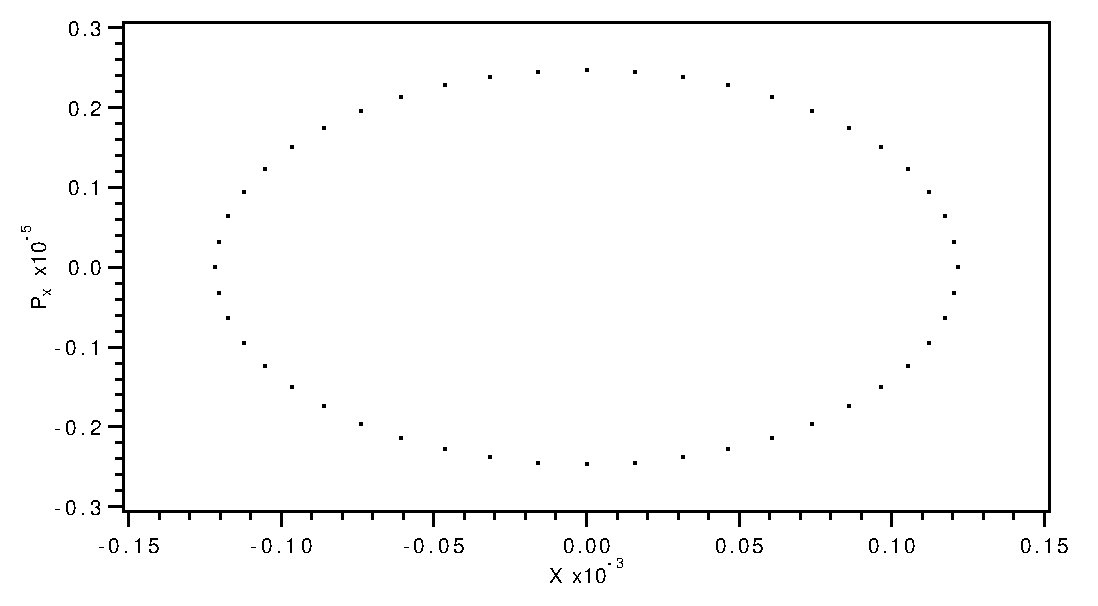
\includegraphics{fig10_7a}
  \caption{Horizontal projection of phase-space initial conditions data
(taken from file 14) as a result of invoking the line {\em makeic} in
{\em \#labor}.}
\end{figure}

\newpage
\begin{figure}[htbp]
\renewcommand{\thefigure}{\thesection.\arabic{figure}}
  \centering
  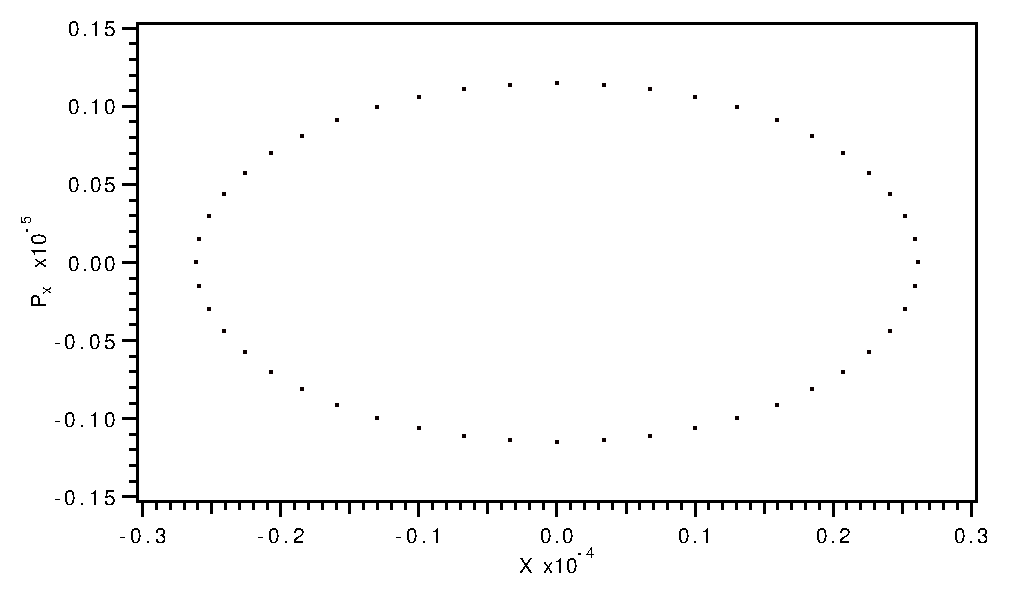
\includegraphics{fig10_7b}
  \caption{Vertical projection of phase-space initial conditions data
(taken from file 14) as a result of invoking the line {\em makeic} in
{\em \#labor}.}
\end{figure}

\newpage
\begin{figure}[htbp]
\renewcommand{\thefigure}{\thesection.\arabic{figure}}
  \centering
  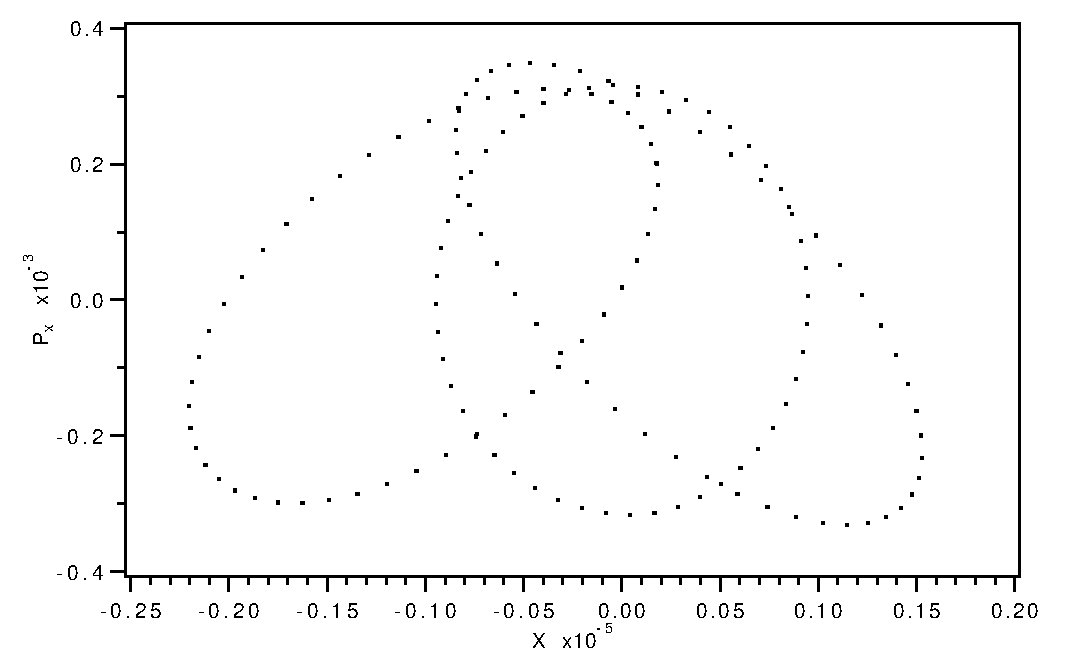
\includegraphics{fig10_8a}
  \caption{Horizontal projection of phase-space final conditions data
computed using the net transfer map for the entire system.}
\end{figure}

\newpage
\begin{figure}[htbp]
\renewcommand{\thefigure}{\thesection.\arabic{figure}}
  \centering
  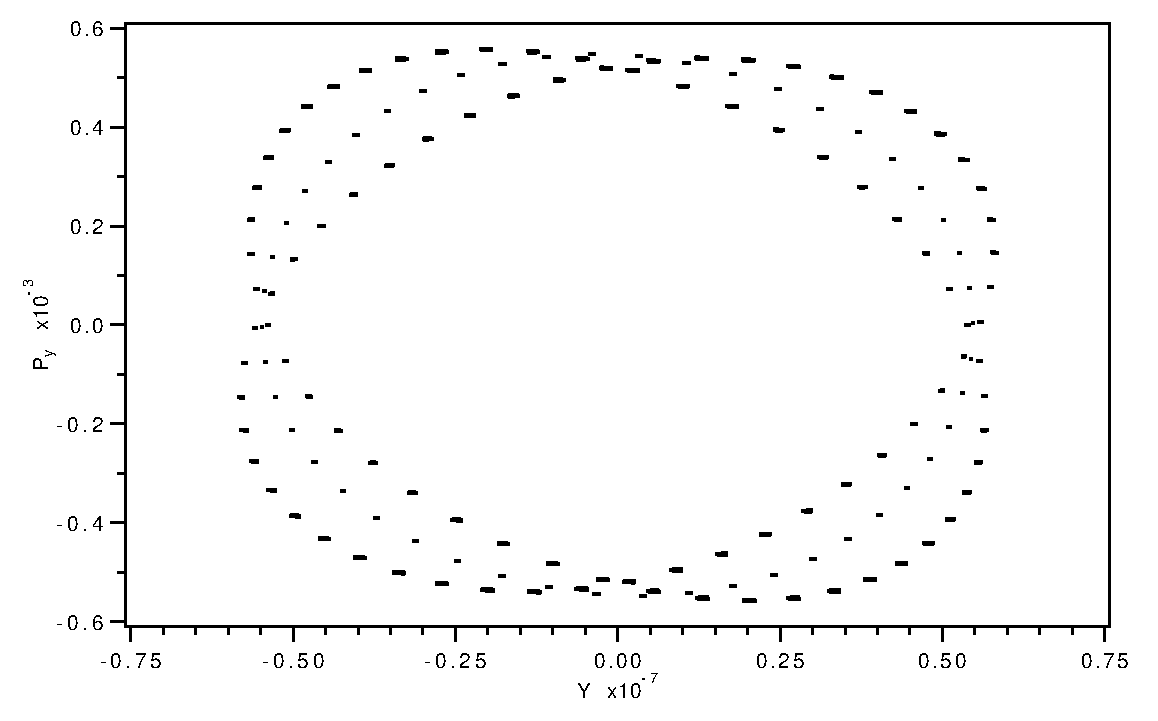
\includegraphics{fig10_8b}
  \caption{Vertical projection of phase-space final conditions data
computed using the net transfer map for the entire system.}
\end{figure}

\newpage
\begin{figure}[htbp]
\renewcommand{\thefigure}{\thesection.\arabic{figure}}
  \centering
  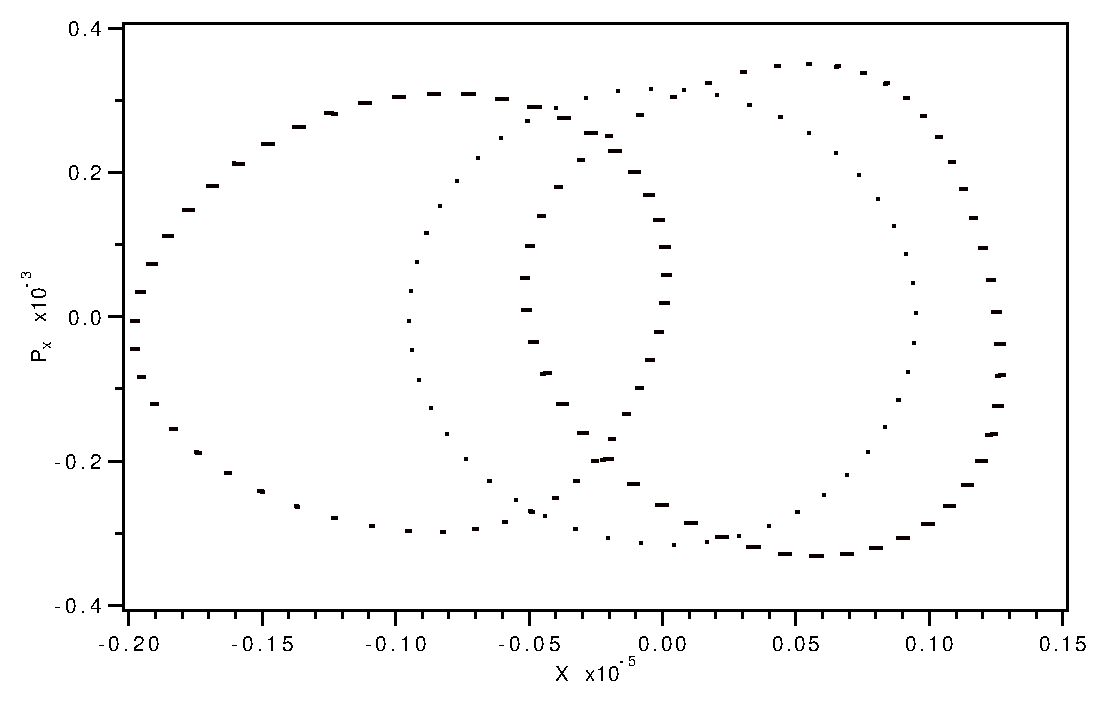
\includegraphics{fig10_9a}
  \caption{Horizontal projection of phase-space final conditions data
computed using element-by-element tracking.}
\end{figure}

\newpage
\begin{figure}[htbp]
\renewcommand{\thefigure}{\thesection.\arabic{figure}}
  \centering
  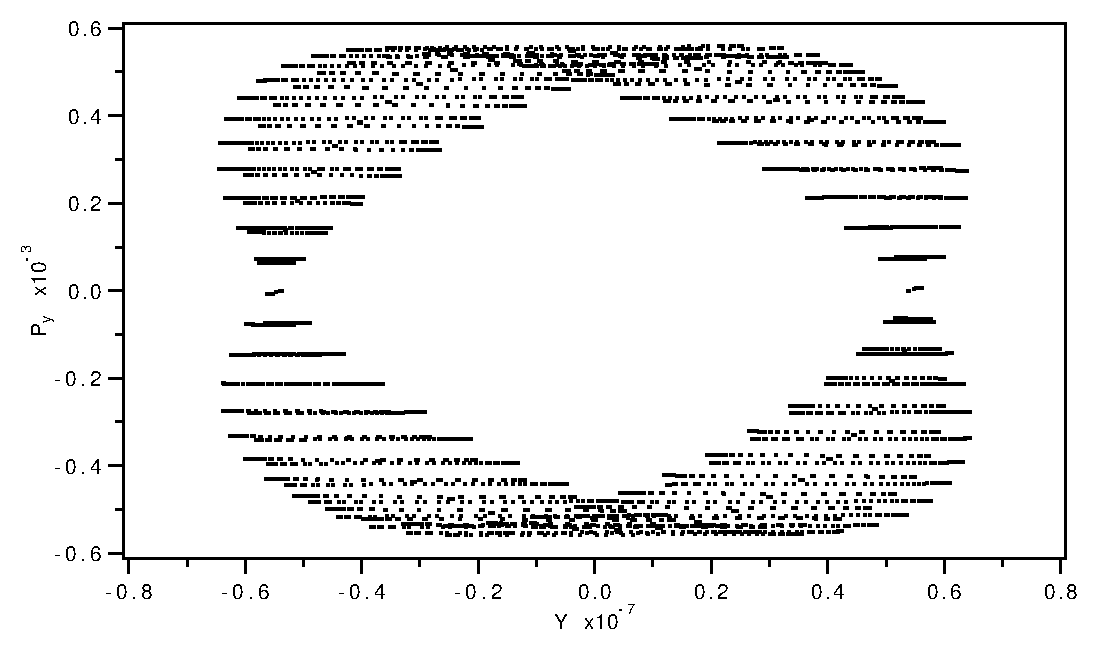
\includegraphics{fig10_9b}
  \caption{Vertical projection of phase-space final conditions data
computed using element-by-element tracking.}
\end{figure}

\newpage
\begin{footnotesize}
\begin{verbatim}
Exhibit 10.7a
***MARYLIE 3.0***
Prerelease Development Version 8/21/98
Copyright 1987 Alex J. Dragt
All rights reserved

Data input complete; going into #labor.
#comment
Exhibit 10.7.1.
     This is a study of the SLAC FFTB facility.  This run does 4
things:

 a) It generates the initial conditions for an input beam.
    This is done by invoking the line makeic in #labor.

 b) It computes the transfer map for the whole system.

 c) It applies this map to the input beam to generate an
    output beam.

 d) To provide an extimate of the effect of higher-order
    aberrations, it also carries out an element-by-element
    ray trace.

The #beam parameters are those for 50 GeV electrons.

#beam
  166.782047599076
  97845.7070864890
  1.00000000000000
  1.00000000000000
#menu
 bgen     bgen
   8.00000000000000       123.000000000000       2304.00000000000
   123.000000000000       1.00000000000000       1.00000000000000
 mom      ps1
  1.500000000000000E-10  1.500000000000000E-11  0.000000000000000E+00
  0.000000000000000E+00  0.000000000000000E+00  0.000000000000000E+00
 pt+      tic
  0.000000000000000E+00  0.000000000000000E+00  0.000000000000000E+00
  0.000000000000000E+00  0.000000000000000E+00  4.000000000000000E-03
 pt-      tic
  0.000000000000000E+00  0.000000000000000E+00  0.000000000000000E+00
  0.000000000000000E+00  0.000000000000000E+00 -8.000000000000000E-03
 twx      twsm
   1.00000000000000       290.000000000000      0.000000000000000E+00
   49.2880000000000
 twy      twsm
   2.00000000000000       31.0000000000000      0.000000000000000E+00
   22.7530000000000
 snor     snor
  0.000000000000000E+00  0.000000000000000E+00  0.000000000000000E+00
  0.000000000000000E+00  0.000000000000000E+00
 gbuf1    gbuf
   2.00000000000000       1.00000000000000
 xform    rt
  0.000000000000000E+00   14.0000000000000       3.00000000000000
  0.000000000000000E+00   1.00000000000000      0.000000000000000E+00
 raysin   rt
   14.0000000000000       14.0000000000000      -1.00000000000000
  0.000000000000000E+00  0.000000000000000E+00  0.000000000000000E+00
 clear    iden
 trace16  rt
  0.000000000000000E+00   16.0000000000000       3.00000000000000
  0.000000000000000E+00   1.00000000000000      0.000000000000000E+00
 circ18   circ
  0.000000000000000E+00   18.0000000000000       5.00000000000000
   1.00000000000000       1.00000000000000       3.00000000000000
 fileout  pmif
   1.00000000000000       12.0000000000000       3.00000000000000
 mapout   ptm
   3.00000000000000       3.00000000000000      0.000000000000000E+00
  0.000000000000000E+00   1.00000000000000
 q81      quad
  7.000000000000001E-02   76.4285271317830       1.00000000000000
   1.00000000000000
 dr01     drft
   13.2483800000000
 q1       quad
  9.367000000000000E-02  -62.0893946731235       1.00000000000000
   1.00000000000000
 dr02     drft
  0.140050000000000
 bpm1     drft
  0.000000000000000E+00
 dr03     drft
   1.62400000000000
 s100     drft
  0.000000000000000E+00
 dr04     drft
   2.68800000000000
 a1x      drft
  0.000000000000000E+00
 dr05     drft
  0.351000000000000
 a1y      drft
  0.000000000000000E+00
 dr06     drft
   4.33553000000000
 b40b1    drft
   1.98120000000000
 dr07     drft
   2.09207000000000
 a2x      drft
  0.000000000000000E+00
 dr08     drft
  0.351000000000000
 a2y      drft
  0.000000000000000E+00
 dr09     drft
  0.382760000000000
 q2       quad
  0.162155000000000       62.0893946731235       1.00000000000000
   1.00000000000000
 dr10     drft
  0.127930000000000
 bpm2     drft
  0.000000000000000E+00
 dr11     drft
   3.21300000000000
 a3x      drft
  0.000000000000000E+00
 dr12     drft
  0.351000000000000
 a3y      drft
  0.000000000000000E+00
 dr13     drft
  0.487100000000000
 q3       quad
  0.143255000000000      -62.0893946731235       1.00000000000000
   1.00000000000000
 dr14     drft
  0.204390000000000
 bpm3     drft
  0.000000000000000E+00
 dr15     drft
  0.580977000000000
 b1       drft
   1.13202700000000
 dr16     drft
  0.761970000000000
 pr2      drft
  0.000000000000000E+00
 dr17     drft
   5.08621300000000
 dr18     drft
   21.8169800000000
 qa01     drft
  5.075000000000000E-02
 dr19     drft
  0.406300000000000
 qa02     drft
  5.075000000000000E-02
 dr20     drft
  0.562626000000000
 pmv      drft
  0.000000000000000E+00
 dr21     drft
   1.09849920000000
 pm1      drft
  0.000000000000000E+00
 dr22     drft
   4.90240320000000
 pm3      drft
  0.000000000000000E+00
 dr23     drft
   4.90198160000000
 b2       drft
  0.000000000000000E+00
 dr24     drft
   65.8979512800000
 d10      drft
   4.26085000000000
 lx0      drft
  0.200000000000000
 lx1      drft
  0.300000000000000
 lx5      drft
  0.500000000000000
 dm0      drft
   7.70439912000000
 dm1      drft
   3.53897240000000
 dm2      drft
  0.561408100000000
 dm3      drft
  0.152400000000000
 dm4      drft
   9.21146240000000
 dm5      drft
  0.561378900000000
 dm6      drft
  0.567588400000000
 swall    drft
   16.7640000000000
 dm7      drft
  0.203200000000000
 dm8      drft
   1.53908000000000
 d2       drft
  0.609600000000000
 st60     drft
  0.609600000000000
 st61     drft
  0.609600000000000
 dmoni    drft
  9.525000000000000E-03
 q5       quad
  0.230460000000000      -19.2771304347826       1.00000000000000
   1.00000000000000
 q6       quad
  0.230460000000000       35.4012173913043       1.00000000000000
   1.00000000000000
 qa0      quad
  0.230460000000000      -24.8659130434783       1.00000000000000
   1.00000000000000
 qa1      quad
  0.230460000000000      -86.9565217391304       1.00000000000000
   1.00000000000000
 qa2      quad
  0.230460000000000       31.2483478260870       1.00000000000000
   1.00000000000000
 dws1     drft
  0.152400000000000
 dws2     drft
  0.304800000000000
 ws       drft
  0.104775000000000
 ws1      mark
 mccsx    mark
 b01      pbnd
  0.216215560584730      0.000000000000000E+00  0.500000000000000
  0.239947000000000
 la1      drft
   1.00000000000000
 la2      drft
   4.95822000000000
 ln1      drft
   5.69811000000000
 ln2      drft
  0.439340000000000
 qn1      quad
  0.230460000000000       75.9993043478261       1.00000000000000
   1.00000000000000
 qn2      quad
  0.230460000000000      -77.6042608695652       1.00000000000000
   1.00000000000000
 qn3      quad
  0.230460000000000       40.9167826086957       1.00000000000000
   1.00000000000000
 sf1      sext
  6.250000000000000E-02   5703.26378000000
 lt1      drft
   3.00000000000000
 lt2      drft
   7.41409000000000
 lt3      drft
   7.54059000000000
 qt1      quad
  0.230460000000000       74.5672173913044       1.00000000000000
   1.00000000000000
 qt2      quad
  0.230460000000000      -62.5448695652174       1.00000000000000
   1.00000000000000
 qt3      quad
  0.230460000000000       80.5043478260870       1.00000000000000
   1.00000000000000
 qt4      quad
  0.230460000000000      -36.8060869565217       1.00000000000000
   1.00000000000000
 b02      pbnd
 -0.216215560584730      0.000000000000000E+00  0.500000000000000
 -0.239947000000000
 qm1      quad
  0.230460000000000       77.6042608695652       1.00000000000000
   1.00000000000000
 qm2      quad
  0.230460000000000      -75.9993043478261       1.00000000000000
   1.00000000000000
 qm3      quad
  0.230460000000000      -40.9167826086957       1.00000000000000
   1.00000000000000
 sd1      sext
  6.250000000000000E-02   6069.09800000000
 lb2      drft
   1.26077000000000
 vcor     drft
  5.000000000000000E-02
 lb3      drft
   8.63923000000000
 lb1      drft
   2.50612000000000
 mff      mark
 pmip     drft
  0.000000000000000E+00
 b03      pbnd
 -2.758937360080000E-02  0.000000000000000E+00  0.500000000000000
 -3.047810000000000E-02
 lb0      drft
   4.96078000000000
 hcor     drft
  5.000000000000000E-02
 lb00     drft
  0.168610000000000
 lc4      drft
   10.3637400000000
 lc3      drft
   4.87095000000000
 lc2      drft
  0.889270000000000
 lxc      drft
  0.150000000000000
 lstar    drft
  0.400000000000000
 qc5      quad
  0.230460000000000      -65.8373913043478       1.00000000000000
   1.00000000000000
 qc4      quad
  0.230460000000000       4.94034782608696       1.00000000000000
   1.00000000000000
 qc3      quad
  0.233500000000000      -44.7427428571429       1.00000000000000
   1.00000000000000
 qc2      quad
   1.00000000000000       40.4418148148148       1.00000000000000
   1.00000000000000
 qx1      quad
  0.150000000000000      -140.000000000000       1.00000000000000
   1.00000000000000
 qc1      quad
  0.550000000000000      -175.384615384615       1.00000000000000
   1.00000000000000
 qs1      quad
  0.230460000000000      0.000000000000000E+00   1.00000000000000
   1.00000000000000
 qs2      quad
  0.230460000000000      0.000000000000000E+00   1.00000000000000
   1.00000000000000
 ftp      mark
 end      end
#lines
 dist
     1*mom         1*bgen
 tws
     1*clear       1*twx         1*twy
 makeic
     1*dist        1*tws         1*snor        1*gbuf1       1*mapout   &
     1*xform       1*pt+         1*xform       1*pt-         1*xform    &
     1*raysin      1*clear
 ltff
     1*q81         1*dr01        2*q1          1*dr02        1*bpm1     &
     1*dr03        1*s100        1*dr04        1*a1x         1*dr05     &
     1*a1y         1*dr06        2*b40b1       1*dr07        1*a2x      &
     1*dr08        1*a2y         1*dr09        2*q2          1*dr10     &
     1*bpm2        1*dr11        1*a3x         1*dr12        1*a3y      &
     1*dr13        2*q3          1*dr14        1*bpm3        1*dr15     &
     2*b1          1*dr16        1*pr2         1*dr17        1*dr18     &
     2*qa01        1*dr19        2*qa02        1*dr20        1*pmv      &
     1*dr21        1*pm1         1*dr22        1*pm3         1*dr23     &
     1*b2          1*dr24        1*d10
 pre
     1*dm0         2*q5          1*dm1         2*q6          1*dm2      &
     2*d2          1*dm3         2*st60        1*dm4         2*st61     &
     1*dm5         2*qa0         1*dm6         2*dmoni       1*swall    &
     1*dm7         2*qa1         1*dm8         2*qa2         1*dws1     &
     1*ws          1*ws1         1*ws          1*dws2
 b0b
     1*b02         1*lx1         1*b02
 b0a
     1*b01         1*lx1         1*b01
 itrm
     2*qt1         1*lt1         2*qt2         1*lx0         2*qt2      &
     1*lt2         2*qt3         1*lt3         2*qt4
 xcc
     1*lx0         4*sf1         1*lx0         2*qn3         1*ln1      &
     2*qn2         1*ln2         1*b0a         1*lx5
 ccsx
     1*b0a         1*la1         2*qn2         1*la2         2*qn3      &
     1*xcc         2*qn1        -1*xcc
 ycc2
     2*sd1         1*lx0         2*qm3         1*ln1         2*qm1      &
     1*ln2         1*b0b         1*lx5
 ccsy
     1*lx0         2*sd1         1*ycc2        2*qm2        -1*ycc2     &
     2*sd1         1*lx0         2*qm3         1*lb3         2*vcor     &
     1*lb2         2*qm1         1*lb1
 sb
     1*b03         1*lx1         1*b03
 ft
     2*qs1         1*lx0         2*qc5         1*lb0         2*hcor     &
     1*lb00        1*b0b         1*lx1         1*sb          1*lx1      &
     2*qc4         1*lc4         2*qs2         1*lx0         2*qc3      &
     1*lc3         1*qc2         1*qc2         1*lc2         2*qx1      &
     1*lxc         2*qc1         1*lstar       1*pmip
 fftb
     1*pre         1*ccsx        1*itrm        1*ccsy        1*ft
 whole
     1*ltff        1*fftb
#lumps
#loops
 onebyone
     1*whole
#labor
    1*fileout
    1*makeic
    1*whole
    1*mapout
    1*trace16
    1*clear
    1*onebyone
    1*circ18
    1*end

****************************************************
* Response to the command bgen in the line makeic: *
****************************************************

       2304 rays generated

 numerically computed values of selected moments
 values of <x*x>, <x*px>, <px*px>:
 1.500000000000011E-010 -2.664596835413195E-026  1.500000000000018E-010
 values of <y*y>, <y*py>, <py*py>:
 1.499999999999989E-011  5.402820688647018E-028  1.499999999999990E-011
 values of <t*t>, <t*pt>, <pt*pt>:
 0.000000000000000E+000  0.000000000000000E+000  0.000000000000000E+000

 analytically computed values of selected moments
 values of <x*x>, <x*px>, <px*px>:
 1.500000000000000E-010  0.000000000000000E+000  1.500000000000000E-010
 values of <y*y>, <y*py>, <py*py>:
 1.500000000000000E-011  0.000000000000000E+000  1.500000000000000E-011
 values of <t*t>, <t*pt>, <pt*pt>:
 0.000000000000000E+000  0.000000000000000E+000  0.000000000000000E+000

******************************
* The matching map script A: *
******************************

matrix for map is :

 7.02054E+00  0.00000E+00  0.00000E+00  0.00000E+00  0.00000E+00  0.00000E+00
 0.00000E+00  1.42439E-01  0.00000E+00  0.00000E+00  0.00000E+00  0.00000E+00
 0.00000E+00  0.00000E+00  4.77001E+00  0.00000E+00  0.00000E+00  0.00000E+00
 0.00000E+00  0.00000E+00  0.00000E+00  2.09643E-01  0.00000E+00  0.00000E+00
 0.00000E+00  0.00000E+00  0.00000E+00  0.00000E+00  1.00000E+00  0.00000E+00
 0.00000E+00  0.00000E+00  0.00000E+00  0.00000E+00  0.00000E+00  1.00000E+00

nonzero elements in generating polynomial are :

****************************
* Reading in matched beam: *
****************************

 6912 ray(s) read in from file  14

**********************************
* Transfer map for whole system: *
**********************************

matrix for map is :

 1.16042E-03  3.80255E-01  0.00000E+00  0.00000E+00  0.00000E+00 -6.52656E-07
-2.57205E+00  1.89289E+01  0.00000E+00  0.00000E+00  0.00000E+00  5.22049E-07
 0.00000E+00  0.00000E+00 -7.92903E-04  4.41560E-02  0.00000E+00  0.00000E+00
 0.00000E+00  0.00000E+00 -1.94231E+01 -1.79537E+02  0.00000E+00  0.00000E+00
 1.67806E-06 -1.25526E-05  0.00000E+00  0.00000E+00  1.00000E+00 -1.17060E-03
 0.00000E+00  0.00000E+00  0.00000E+00  0.00000E+00  0.00000E+00  1.00000E+00

nonzero elements in generating polynomial are :

 f( 28)=f( 30 00 00 )=-3.89227825816134E-02
 f( 29)=f( 21 00 00 )= 8.82503434730550E-02
 f( 33)=f( 20 00 01 )= -913.33367251839
 f( 34)=f( 12 00 00 )=-6.28096901842339E-02
 f( 38)=f( 11 00 01 )=  13.817825821166
 f( 39)=f( 10 20 00 )= 5.30573201601003E-02
 f( 40)=f( 10 11 00 )= 0.11077558702035
 f( 43)=f( 10 02 00 )= 3.51466442021233E-03
 f( 48)=f( 10 00 02 )= 0.45425928722257
 f( 49)=f( 03 00 00 )=-1.15123554435159E-04
 f( 53)=f( 02 00 01 )= 0.28123701550681
 f( 54)=f( 01 20 00 )=-0.54577103156849
 f( 55)=f( 01 11 00 )=-7.11881814520230E-02
 f( 58)=f( 01 02 00 )= 4.16651091578457E-05
 f( 63)=f( 01 00 02 )= 2.10706864800540E-02
 f( 67)=f( 00 20 01 )= -7607.4908656048
 f( 70)=f( 00 11 01 )=  4.0703495464613
 f( 76)=f( 00 02 01 )= 3.78505599207130E-03
 f( 83)=f( 00 00 03 )= 7.16372329713475E-04
 f( 84)=f( 40 00 00 )= -1509577.7880829
 f( 85)=f( 31 00 00 )=  31525.584758041
 f( 89)=f( 30 00 01 )=  1051.3749913900
 f( 90)=f( 22 00 00 )= -102.70479343622
 f( 94)=f( 21 00 01 )= -3117.6407533003
 f( 95)=f( 20 20 00 )= -41749615.002048
 f( 96)=f( 20 11 00 )= -823.45497555658
 f( 99)=f( 20 02 00 )= -12.024976325221
 f(104)=f( 20 00 02 )= -8215.8059409657
 f(105)=f( 13 00 00 )= -548.24879728467
 f(109)=f( 12 00 01 )=  2317.1974918641
 f(110)=f( 11 20 00 )=  166247.09590690
 f(111)=f( 11 11 00 )=  67.126217696816
 f(114)=f( 11 02 00 )= -7.8306638896465
 f(119)=f( 11 00 02 )=  593.63080145352
 f(123)=f( 10 20 01 )=  3977.3635330146
 f(126)=f( 10 11 01 )= -612.91427242861
 f(132)=f( 10 02 01 )= -173.87987518916
 f(139)=f( 10 00 03 )= -8.5049112006986
 f(140)=f( 04 00 00 )=  200.25538481841
 f(144)=f( 03 00 01 )= 0.89850794460257
 f(145)=f( 02 20 00 )= -249.70141545497
 f(146)=f( 02 11 00 )=  139.41365645640
 f(149)=f( 02 02 00 )=  5.9698255205061
 f(154)=f( 02 00 02 )=  5.2855306317948
 f(158)=f( 01 20 01 )= -18326.626444905
 f(161)=f( 01 11 01 )= -2655.4851662894
 f(167)=f( 01 02 01 )=-6.39318206821628E-02
 f(174)=f( 01 00 03 )= -10.589966794531
 f(175)=f( 00 40 00 )= -95434657.276104
 f(176)=f( 00 31 00 )=  30603.630699873
 f(179)=f( 00 22 00 )=  1516.9195509404
 f(184)=f( 00 20 02 )= -41485.878055000
 f(185)=f( 00 13 00 )=  147.03874397650
 f(190)=f( 00 11 02 )= -34.314062493911
 f(195)=f( 00 04 00 )=  5.0709745286033
 f(200)=f( 00 02 02 )= 1.72432221019481E-05
 f(209)=f( 00 00 04 )=-2.45235185866578E-02

*******************************************************
* Elements traversed in element-by-element ray trace: *
*******************************************************

circulating through onebyone :
 q81      dr01     q1       q1       dr02
 bpm1     dr03     s100     dr04     a1x
 dr05     a1y      dr06     b40b1    b40b1
 dr07     a2x      dr08     a2y      dr09
 q2       q2       dr10     bpm2     dr11
 a3x      dr12     a3y      dr13     q3
 q3       dr14     bpm3     dr15     b1
 b1       dr16     pr2      dr17     dr18
 qa01     qa01     dr19     qa02     qa02
 dr20     pmv      dr21     pm1      dr22
 pm3      dr23     b2       dr24     d10
 dm0      q5       q5       dm1      q6
 q6       dm2      d2       d2       dm3
 st60     st60     dm4      st61     st61
 dm5      qa0      qa0      dm6      dmoni
 dmoni    swall    dm7      qa1      qa1
 dm8      qa2      qa2      dws1     ws
 ws1      ws       dws2     b01      lx1
 b01      la1      qn2      qn2      la2
 qn3      qn3      lx0      sf1      sf1
 sf1      sf1      lx0      qn3      qn3
 ln1      qn2      qn2      ln2      b01
 lx1      b01      lx5      qn1      qn1
 lx5      b01      lx1      b01      ln2
 qn2      qn2      ln1      qn3      qn3
 lx0      sf1      sf1      sf1      sf1
 lx0      qt1      qt1      lt1      qt2
 qt2      lx0      qt2      qt2      lt2
 qt3      qt3      lt3      qt4      qt4
 lx0      sd1      sd1      sd1      sd1
 lx0      qm3      qm3      ln1      qm1
 qm1      ln2      b02      lx1      b02
 lx5      qm2      qm2      lx5      b02
 lx1      b02      ln2      qm1      qm1
 ln1      qm3      qm3      lx0      sd1
 sd1      sd1      sd1      lx0      qm3
 qm3      lb3      vcor     vcor     lb2
 qm1      qm1      lb1      qs1      qs1
 lx0      qc5      qc5      lb0      hcor
 hcor     lb00     b02      lx1      b02
 lx1      b03      lx1      b03      lx1
 qc4      qc4      lc4      qs2      qs2
 lx0      qc3      qc3      lc3      qc2
 qc2      lc2      qx1      qx1      lxc
 qc1      qc1      lstar    pmip

end of MARYLIE run


Exhibit 10.7b
Contents of file 9 that provides desired second
moments for the command moma:

6 6  0
7     .73932e-8
13   3.04333712059731e-12
18   3.41295e-10
22    .659253724783545e-12
209  0


Exhibit 10.7c
***MARYLIE 3.0***
Prerelease Development Version 1/12/00
Copyright 1987 Alex J. Dragt
All rights reserved

Data input complete; going into #labor.
#comment
Exhibit 10.7c
     This MaryLie run exhibits the use of the moma command
to generate a matched beam given a set of moments.

Although immaterial for this purpose, the #beam parameters are
those for 50 GeV electrons.

#beam
  166.782047599076
  97845.7070864890
  1.00000000000000
  1.00000000000000
#menu
 moma     moma
   21.0000000000000       1.00000000000000       9.00000000000000
   1.00000000000000      0.000000000000000E+00  0.000000000000000E+00
 bgen     bgen
   8.00000000000000       123.000000000000       2304.00000000000
   123.000000000000       1.00000000000000       1.00000000000000
 mom      ps1
  -1.00000000000000      0.000000000000000E+00  0.000000000000000E+00
  0.000000000000000E+00  0.000000000000000E+00  0.000000000000000E+00
 pt+      tic
  0.000000000000000E+00  0.000000000000000E+00  0.000000000000000E+00
  0.000000000000000E+00  0.000000000000000E+00  4.000000000000000E-03
 pt-      tic
  0.000000000000000E+00  0.000000000000000E+00  0.000000000000000E+00
  0.000000000000000E+00  0.000000000000000E+00 -8.000000000000000E-03
 gbuf1    gbuf
   2.00000000000000       1.00000000000000
 mask     mask
   1.00000000000000      0.000000000000000E+00  0.000000000000000E+00
  0.000000000000000E+00  0.000000000000000E+00  0.000000000000000E+00
 xform    rt
  0.000000000000000E+00   14.0000000000000       3.00000000000000
  0.000000000000000E+00   1.00000000000000      0.000000000000000E+00
 raysin   rt
   14.0000000000000       14.0000000000000      -1.00000000000000
  0.000000000000000E+00  0.000000000000000E+00  0.000000000000000E+00
 clear    iden
 trace16  rt
  0.000000000000000E+00   16.0000000000000       3.00000000000000
  0.000000000000000E+00   1.00000000000000      0.000000000000000E+00
 circ18   circ
  0.000000000000000E+00   18.0000000000000       5.00000000000000
   1.00000000000000       1.00000000000000       3.00000000000000
 fileout  pmif
   1.00000000000000       12.0000000000000       3.00000000000000
 mapout   ptm
   3.00000000000000       3.00000000000000      0.000000000000000E+00
  0.000000000000000E+00   1.00000000000000
 end      end
#lines
 dist
     1*mom         1*bgen
 makeic
     1*moma        1*gbuf1       1*mapout      1*dist        1*mask     &
     1*mapout      1*xform       1*pt+         1*xform       1*pt-      &
     1*xform       1*raysin      1*clear
#lumps
#loops
#labor
    1*fileout
    1*makeic
    1*end

****************************************************
* Response to the moma command in the line makeic: *
****************************************************

file unit  9 rewound
map read in from file   9;   0 record(s) skipped
xee2=  2.250000000000006E-020
yee2=  2.250000000000000E-022
tee2=  0.000000000000000E+000

********************************************
* Matrix part of the map produced by moma: *
********************************************

matrix for map is :

 7.02054E+00  0.00000E+00  0.00000E+00  0.00000E+00  0.00000E+00  0.00000E+00
 0.00000E+00  1.42439E-01  0.00000E+00  0.00000E+00  0.00000E+00  0.00000E+00
 0.00000E+00  0.00000E+00  4.77001E+00  0.00000E+00  0.00000E+00  0.00000E+00
 0.00000E+00  0.00000E+00  0.00000E+00  2.09643E-01  0.00000E+00  0.00000E+00
 0.00000E+00  0.00000E+00  0.00000E+00  0.00000E+00  1.00000E+00  0.00000E+00
 0.00000E+00  0.00000E+00  0.00000E+00  0.00000E+00  0.00000E+00  1.00000E+00

*******************************
* Eigenmoments found by moma: *
*******************************

nonzero elements in generating polynomial are :

 f(  7)=f( 20 00 00 )= 1.50000000000000E-10
 f( 13)=f( 02 00 00 )= 1.50000000000000E-10
 f( 18)=f( 00 20 00 )= 1.50000000000000E-11
 f( 22)=f( 00 02 00 )= 1.50000000000000E-11

**************************************************
* Response to the command bgen in the line dist: *
**************************************************

       2304 rays generated

 numerically computed values of selected moments
 values of <x*x>, <x*px>, <px*px>:
 1.500000000000022E-010 -3.136370717220037E-026  1.500000000000018E-010
 values of <y*y>, <y*py>, <py*py>:
 1.499999999999989E-011  5.402820688647018E-028  1.499999999999990E-011
 values of <t*t>, <t*pt>, <pt*pt>:
 0.000000000000000E+000  0.000000000000000E+000  0.000000000000000E+000

 analytically computed values of selected moments
 values of <x*x>, <x*px>, <px*px>:
 1.500000000000002E-010  0.000000000000000E+000  1.500000000000002E-010
 values of <y*y>, <y*py>, <py*py>:
 1.500000000000000E-011  0.000000000000000E+000  1.500000000000000E-011
 values of <t*t>, <t*pt>, <pt*pt>:
 0.000000000000000E+000  0.000000000000000E+000  0.000000000000000E+000

******************************************************
* Map (script A) used to transform the distribution: *
******************************************************

matrix for map is :

 7.02054E+00  0.00000E+00  0.00000E+00  0.00000E+00  0.00000E+00  0.00000E+00
 0.00000E+00  1.42439E-01  0.00000E+00  0.00000E+00  0.00000E+00  0.00000E+00
 0.00000E+00  0.00000E+00  4.77001E+00  0.00000E+00  0.00000E+00  0.00000E+00
 0.00000E+00  0.00000E+00  0.00000E+00  2.09643E-01  0.00000E+00  0.00000E+00
 0.00000E+00  0.00000E+00  0.00000E+00  0.00000E+00  1.00000E+00  0.00000E+00
 0.00000E+00  0.00000E+00  0.00000E+00  0.00000E+00  0.00000E+00  1.00000E+00

nonzero elements in generating polynomial are :

********************************************
* Reading in the transformed distribution: *
********************************************

 6912 ray(s) read in from file  14

end of MARYLIE run
\end{verbatim}
\end{footnotesize}

%\newpage
\section{Calculation of Dynamic Aperture for a Storage Ring}\index{dynamic aperture} \index{storage ring}
\label{aperture}
Accelerator codes that do not use maps typically determine the dynamic
aperture using element-by-element tracking.  Elements such as drifts, bends, and
quads are treated in linear approximation using matrices, and nonlinear elements
are treated as integrated multipole kicks.\index{kicks}  Sometimes even the linear effects
of bends and quads are treated as kicks.  High-order multipole errors in
quads and dipoles are treated by slicing these elements and inserting nonlinear
kicks between the slices.  Sometimes many slices are used.  Often, to speed up
computation (but presumably at the expense of accuracy), only a few slices
are used.  Sometimes kicks which properly should be made along the body of
dipoles (and frequently) are made instead only in quads.

Simulations of the type described above can also be done with \Mary.  One
can easily write user routines (see section 6.20) that kick particles in
any desired manner.  Any element can be sliced at will, and a user routine can
be inserted between any two slices.  For convenience, all the slices and user
routines can be put in a tracking loop, and this loop can be tracked
repeatedly as often as desired with the use of a circ command.  See sections 5.10 and
7.3.

However, wherever possible, it is desirable to make use of maps.  So doing
could speed up dynamic aperture calculations (which are often very
lengthy) by orders of magnitude.  Without any increase in computer time, one could
also use maps that are more accurate than kick approximations.  They could describe
thick elements and could also include fringe-field effects.  Finally, with maps
one might hope for more insight: perhaps various lattices could be compared
without the need for long-term tracking, detrimental terms in maps could be
identified, and correction schemes could be devised to remove them.

It appears that the dynamic aperture for various SSC designs and the CERN
Large Hadron Collider can be determined by symplectic tracking with a
one-turn map.  The same is believed to be true for the Stanford B-Factory rings.
In the case of synchrotron light rings, whose one-turn maps may be more nonlinear,
it may be necessary to use a modest number of lumps.  All these applications
of map methods are still somewhere in the development stage, and require maps
somewhat beyond third order.

Subsection 10.8.1 describes the calculation of a point on the edge of the dynamic aperture of the Tevatron in the case that several families of sextupoles are purposely
strongly powered to reduce the dynamic aperture.  (Experiments of this type were
done on the Tevatron to answer various questions about magnet quality
requirements for the  SSC.)  In this circumstance the dominant
nonlinearities are those produced by the sextupoles, and all other sources of
nonlinearity such as multipole errors in dipoles and quadrupoles become
negligible by comparison.  Correspondingly, it is sufficient to use third-order
maps providing the effect of the one-turn map is approximated by a
sufficient number of lumps.\index{lumps}  The same is true for any ring whose dynamic
aperture is controlled primarily by sextupole and octupole nonlinearities.

Subsection 10.8.2 studies the history of a particle that is just outside
the dynamic aperture, and consequently makes several turns before it is
lost.

\subsection{Dynamic Aperture of Tevatron with Strong Distortion Sextupoles}
\label{teva}
The Tevatron lattice
has 6 sectors labelled A through F as one circles around the ring
clockwise when seen from above.  See figure 10.8.1.1.  The strong
``distortion'' sextupoles described above
are located in
sectors C and F.  Eight of them are placed in each sector.  The beam is
``observed'' (a Poincare surface of section is situated) at the location
of a horizontal position monitor in sector E (by marker e24).\index{Tevatron}

Exhibit 10.8.1 shows the results of a \Mary run designed to find a point
on the edge of the dynamic aperture.  A ``linearly'' matched ``surface''
beam (consisting of 30 particles) is generated randomly and tracked for
10,000 turns.\index{matched beam}  It is found that one particle is lost in this process when
the horizontal and vertical mean-square emittances have the values
\[
\epsilon^2_x = \langle X^2\rangle \langle P^2_x\rangle = (5.31 \times
10^{-8})^2,
\]
\[
\epsilon^2_y = \langle Y^2\rangle \langle P^2_y\rangle = (5.31 \times
10^{-8})^2.
\]
By contrast, when $\epsilon^2_x = \epsilon^2_y = (5.30 \times
10^{-8})^2$, no particles are lost.  Thus, a point on or near the
boundary of the (10,000 turn) dynamic aperture has been determined.
Unlike many tracking studies, the use of a randomly generated matched
surface beam explores the dynamic aperture for many different initial
betatron and synchrotron phases.  Figures 10.8.1.2 through 10.8.1.4 show this
initial beam.  Note that the 2-dimensional projections of the beam lie
on ellipses in the vertical and temporal planes.  However, the horizontal
distribution is spread out because of dispersion at the location of the
horizontal position monitor.

Exhibits 10.8.1a and 10.8.1b show the contents of the {\em istat} and
{\em ihist} arrays at the end of the tracking run.  The {\em istat} array
shows that only particle number 6 is lost, and that loss occurred on turn
427.  The {\em ihist} array shows that the first (and only) particle to
be lost was lost on turn 427, and that particle is the 6th one in the
initial distribution.  Figures 10.8.1.5 through 10.8.1.7 show 2-dimensional
projections of the beam during the course of 10,000 turns with results
written out every 43rd turn.  The effect of dispersion in the horizontal
projection is again evident.  Also, the temporal projection exhibits
synchro-betatron coupling.  Finally, Exhibit 10.8.1c shows the \Mary
run itself.

\newpage
\begin{figure}[htbp]
  \centering
  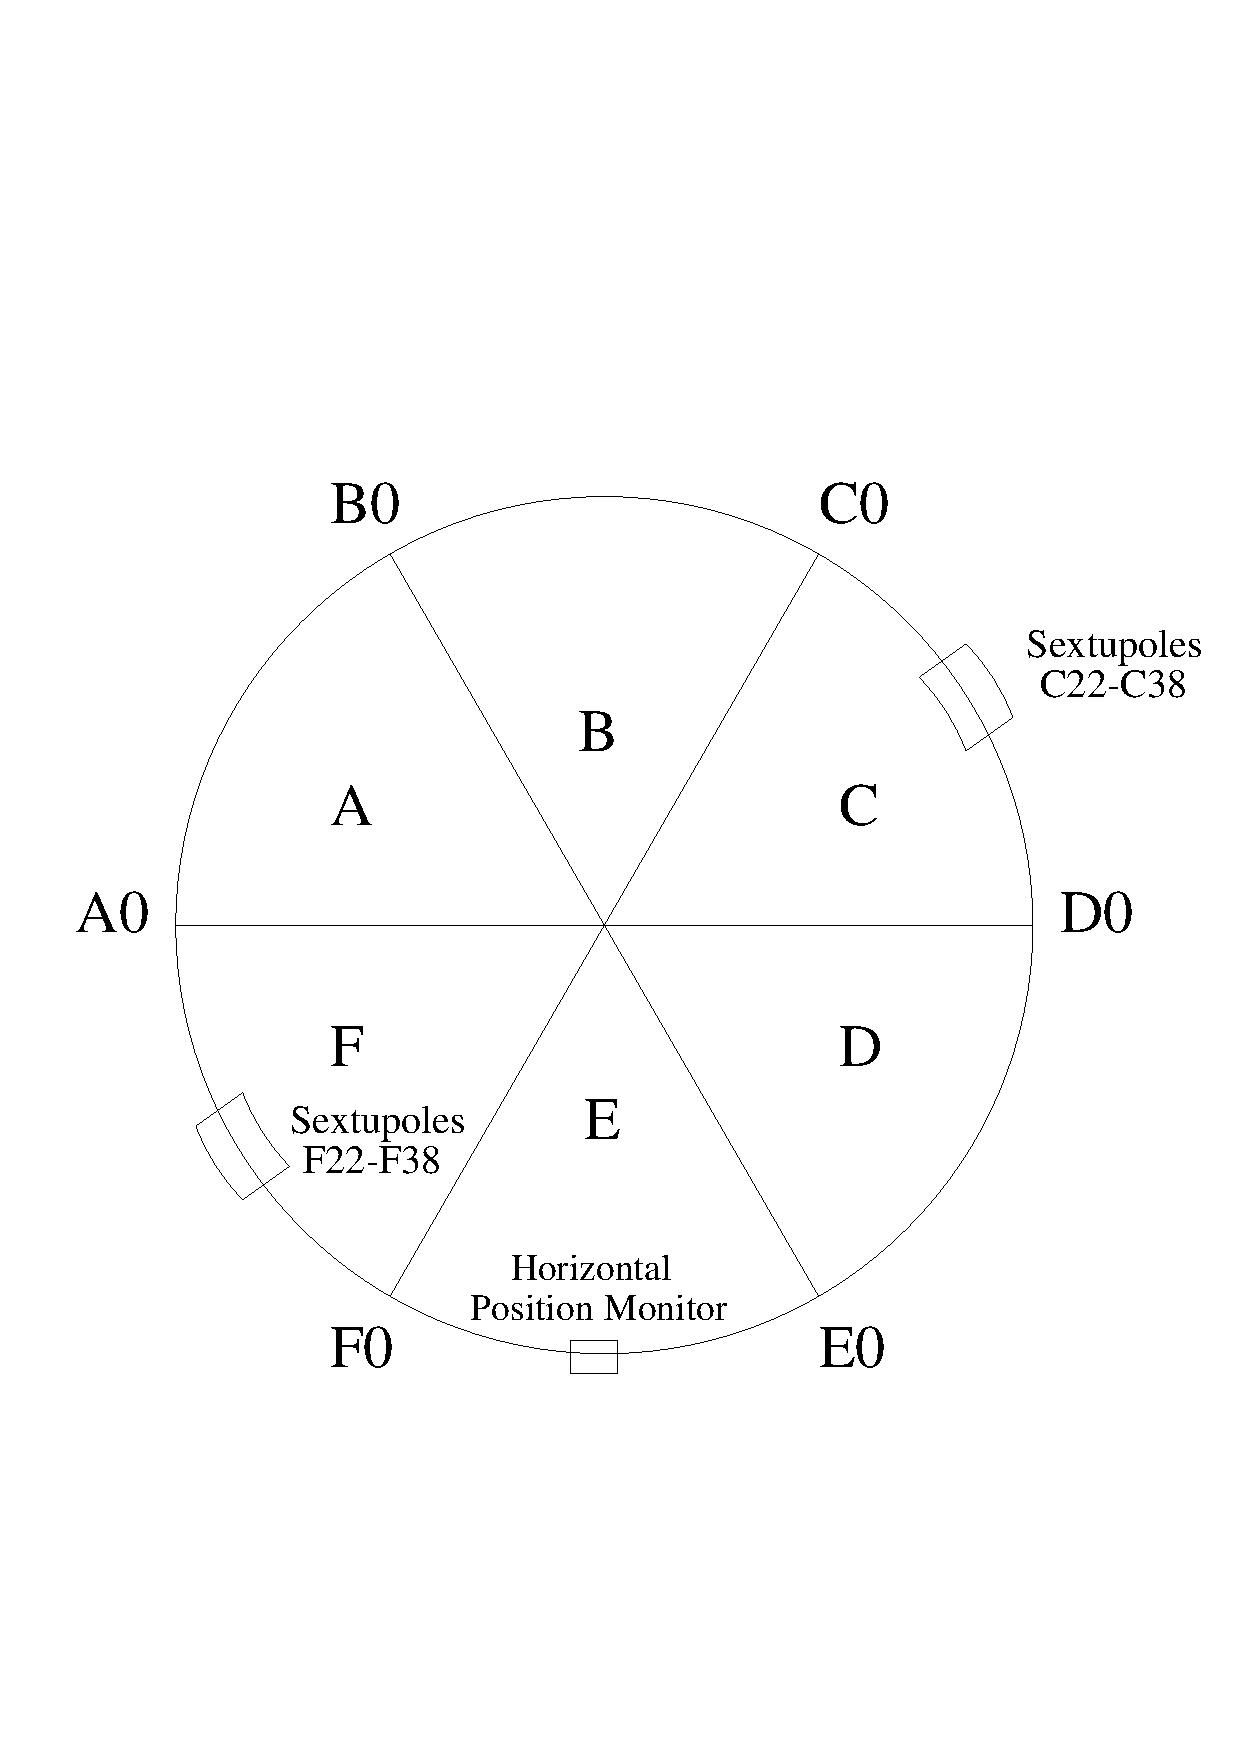
\includegraphics{fig10_10}
  \caption{Schematic layout of the Tevatron lattice.}
\end{figure}

\newpage
\begin{figure}[htbp]
  \centering
  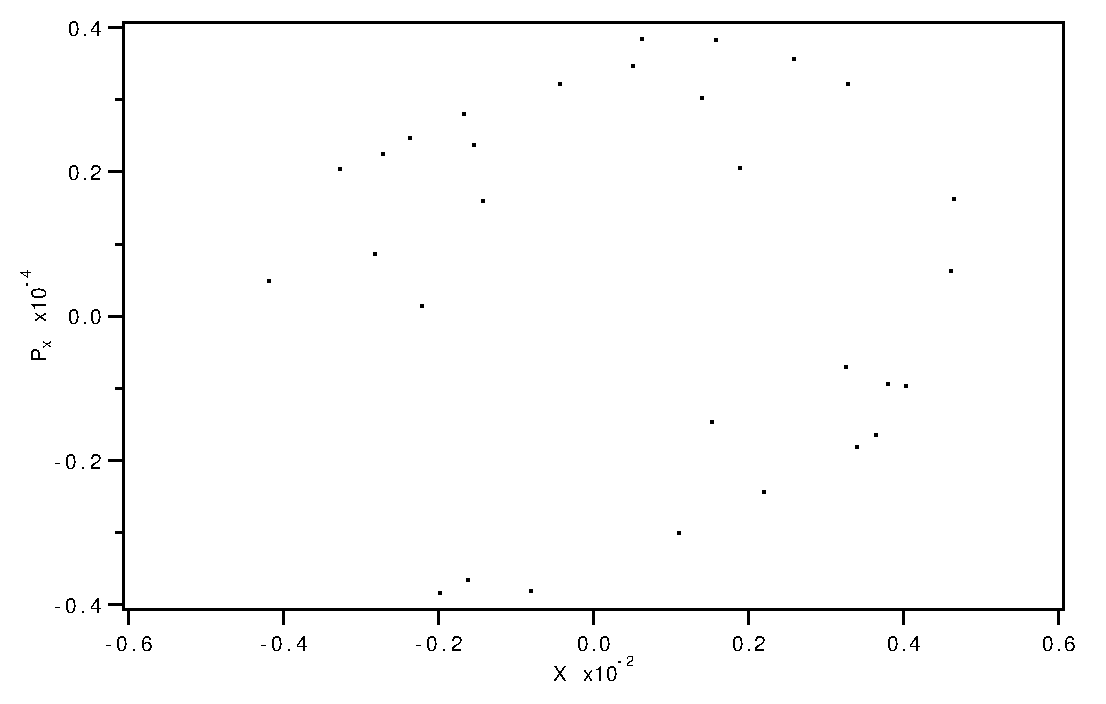
\includegraphics{fig10_11a}
  \caption{Horizontal projection of phase-space initial conditions (file 16).}
\end{figure}

\newpage
\begin{figure}[htbp]
  \centering
  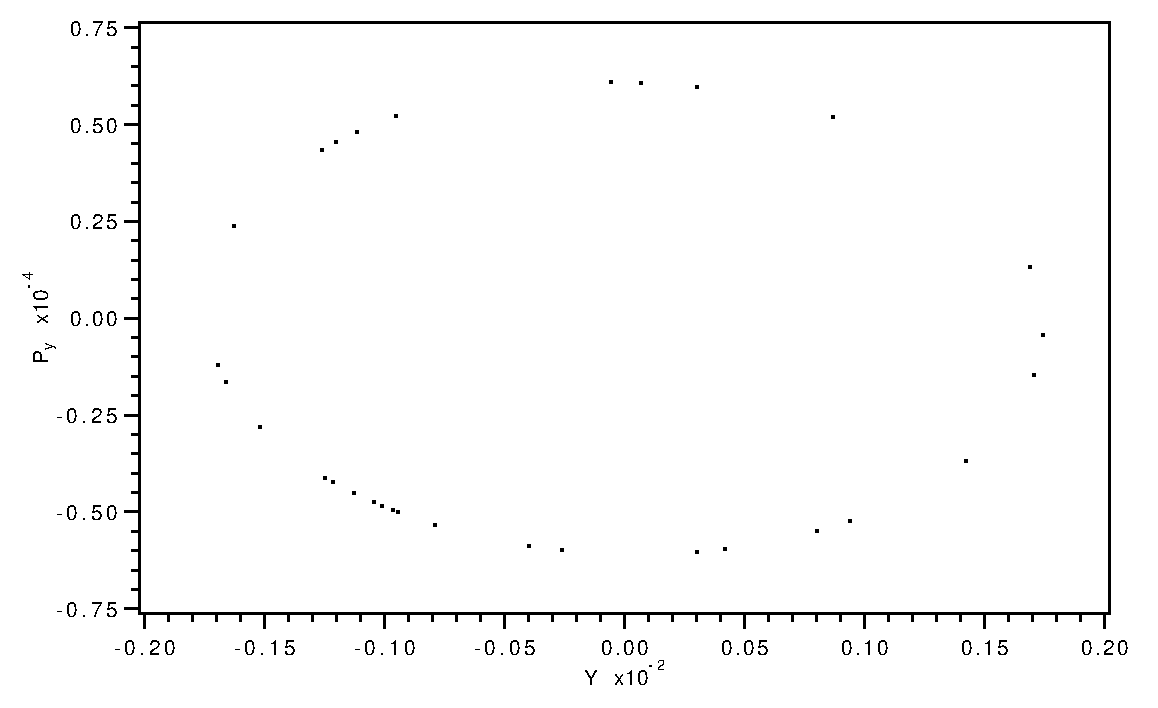
\includegraphics{fig10_11b}
  \caption{Vertical projection of phase-space initial conditions (file 16).}
\end{figure}

\newpage
\begin{figure}[htbp]
  \centering
  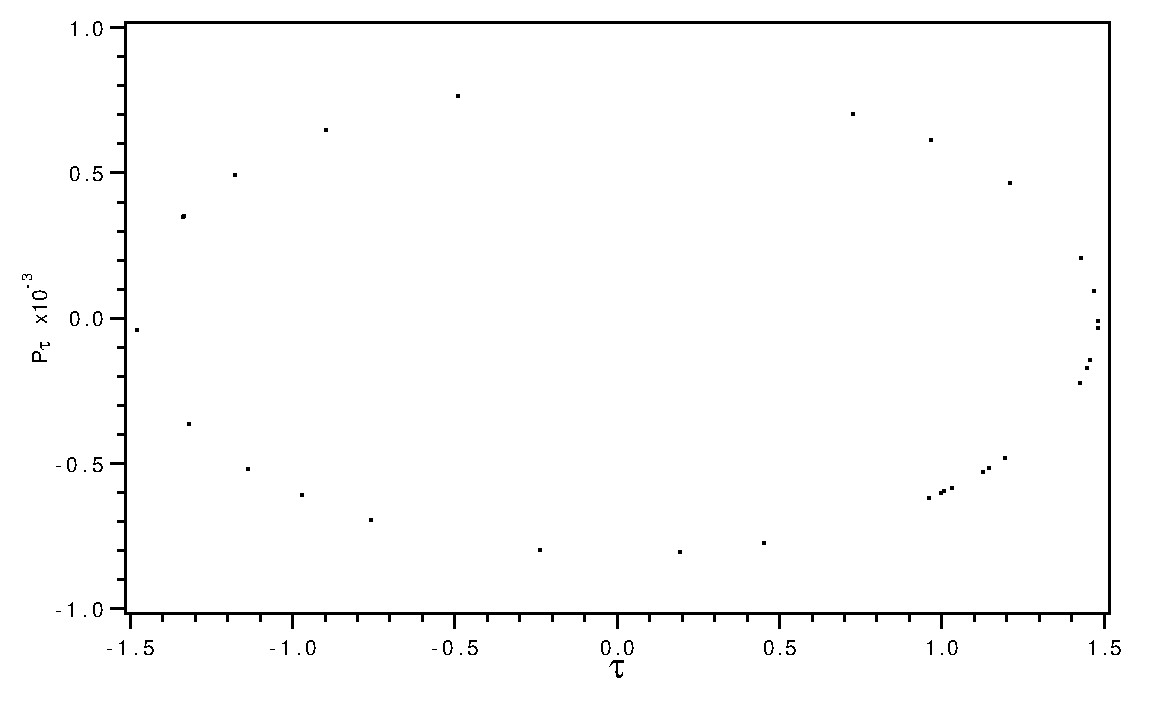
\includegraphics{fig10_11c}
  \caption{Temporal projection of phase-space initial conditions (file 16).}
\end{figure}

\newpage
\begin{figure}[htbp]
  \centering
  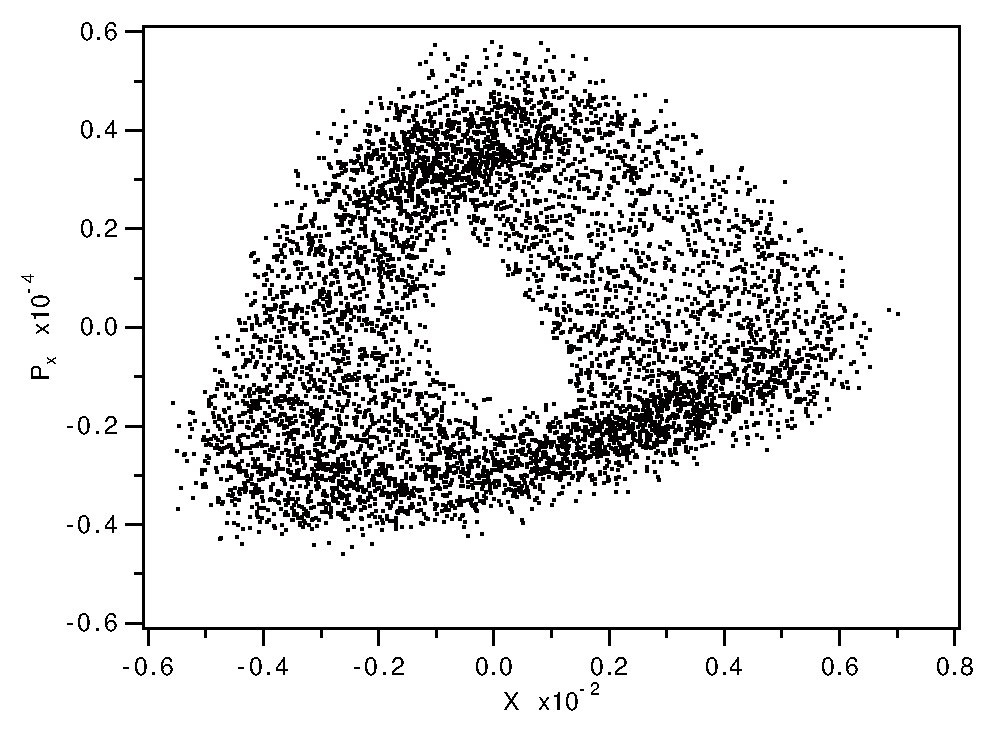
\includegraphics{fig10_12a}
  \caption{Horizontal projection of phase-space tracking data (file 14).}
\end{figure}

\newpage
\begin{figure}[htbp]
  \centering
  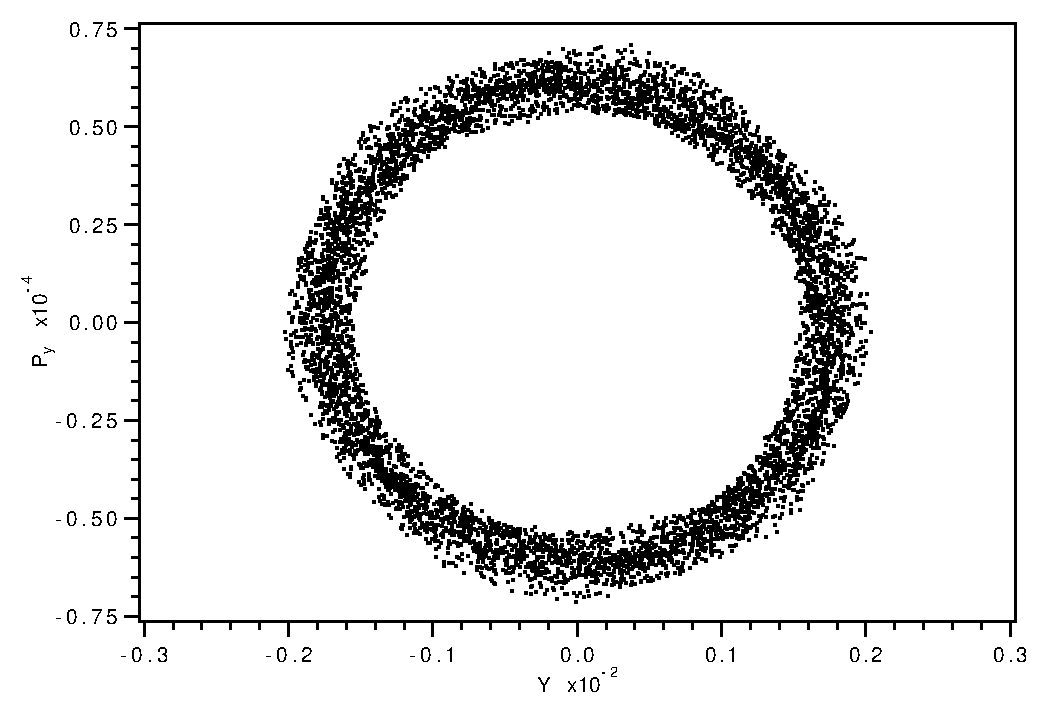
\includegraphics{fig10_12b}
  \caption{Vertical projection of phase-space tracking data (file 14).}
\end{figure}

\newpage
\begin{figure}[htbp]
  \centering
  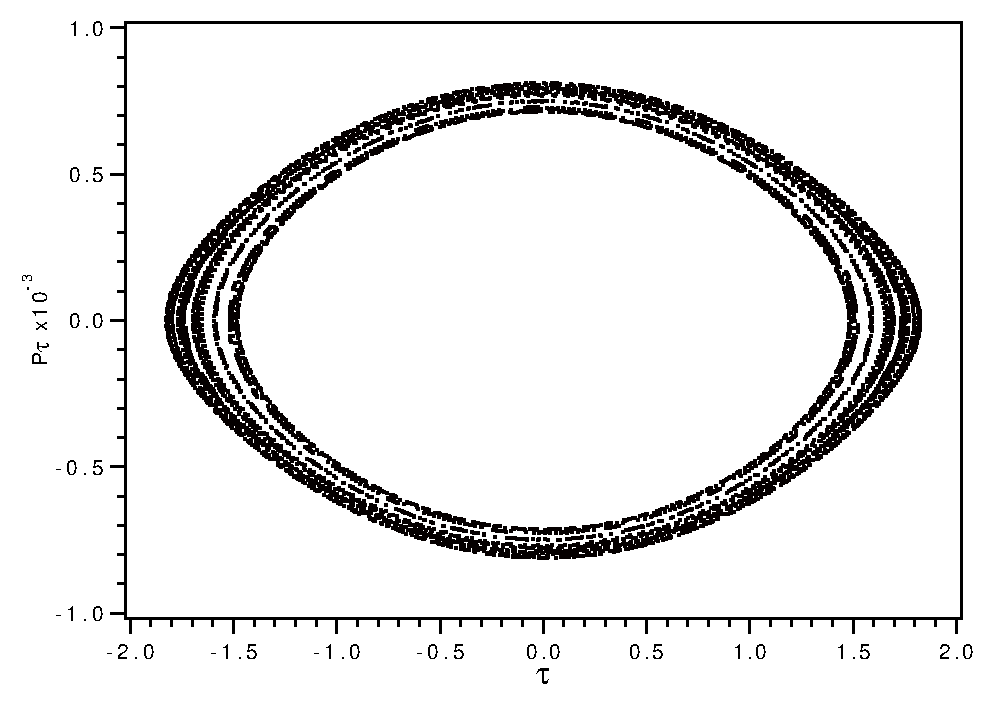
\includegraphics{fig10_12c}
  \caption{Temporal projection of phase-space tracking data (file 14).}
\end{figure}

\newpage
\begin{footnotesize}
\begin{verbatim}
Exhibit 10.8.1a
Contents of file 20, the array istat:

         1         0
         2         0
         3         0
         4         0
         5         0
         6       427
         7         0
         8         0
         9         0
        10         0
        11         0
        12         0
        13         0
        14         0
        15         0
        16         0
        17         0
        18         0
        19         0
        20         0
        21         0
        22         0
        23         0
        24         0
        25         0
        26         0
        27         0
        28         0
        29         0
        30         0


Exhibit 10.8.1b
Contents of file 22, the array ihist:

         1       427         6


Exhibit 10.8.1c
***MARYLIE 3.0***
Prerelease Development Version 8/21/98
Copyright 1987 Alex J. Dragt
All rights reserved

Data input complete; going into #labor.
#comment
Exhibit 10.8.1.
    This is a MARYLIE run to study the dynamic aperture of the Tevatron when
16 distortion sextupoles are powered.  The 'quads' q0c1 and q0c2 are set to
achieve horizontal and vertical tunes of .39 and .46, respectively, and the
'sextupoles' s0c1 and s0c2 are set to achieve zero first-order chromaticities.
Both these fits were made with the RF cavity (rfca) turned off.  In this run
the RF cavity is powered.  As one can see from the response to the tadm
command, the transverse tunes shift slightly when the cavity is turned on due
both to synchro-betatron coupling and the defocussing effects of the cavity.
The distortion sextupoles dsex+ and dsex- are set to strengths corresponding
to 30 amperes  excitation current.  Fringe-field effects are included.
Finally, the beam parameters are those for 150 GeV protons.

This MaryLie run does 10 things:

 a) It computes maps for the lines cxfd and cxdf, which occur
    repeatedly in the Tevatron lattice, and stores them as lumps
    in order to speed up subsequent computations.

 b) It computes 17 transfer maps and writes them out sequentially on file 10.
    The 1st transfer map describes the elements stretching from the location
    of a  horizontal beam position monitor in sector E (location e24) to the
    trailing end of the 1st distortion sextupole.  The 2nd transfer map
    describes the elements from the trailing end of the 1st distortion
    sextupole location to the trailing end of the 2nd distortion
    sextupole. ... The 16th transfer map describes the elements from the
    trailing end of the 15th distortion sextupole location to the trailing
    end of the 16th distortion sextupole.  Finally, the 17th transfer map
    describes the elements from the trailing end of the 16th distortion
    sextupole location back to the horizontal position monitor location.
    Thus, when combined, these 17 transfer maps give a full one-turn map.

 c) It reads these maps back in and stores them as lumps.

 d) These 17 maps are concatenated to give a one-turn map.

 e) A tadm command is used to compute script A and the tunes
    for the one-turn map.

 f) A random uniform distribution of rays is generated on the
    3-dimensional surface of a perfect torus in 6 dimensions.

 g) The "linear" part of script A is gotten from buffer1 and applied
    to these rays to make a "linearly" matched beam.

 h) This matched beam is written in "ordinary" precision on files
    14 and 16, and in full precision on file 18.

 i) This matched beam is tracked lump-by-lump for 10,000 turns
    with results written to file 14 every 43rd turn.

 j) The istat and ihist arrays are written on files 20 and 22,
    respectively.

#beam
  503.466178765432
  159.867058817009
  1.00000000000000
  1.00000000000000
#menu
 bh1      nbnd
  0.465116280536985      0.000000000000000E+00  0.500000000000000
  0.667664755182949       1.00000000000000       1.00000000000000
 bbs      nbnd
  0.222087819188675      0.000000000000000E+00  0.500000000000000
  0.667656760387843       1.00000000000000       1.00000000000000
 bl       nbnd
  0.105114881640705      0.000000000000000E+00  0.500000000000000
  0.163191579283132       1.00000000000000       1.00000000000000
 bc       nbnd
  8.535352727179631E-02  0.000000000000000E+00  0.500000000000000
  0.198175132463878       1.00000000000000       1.00000000000000
 bbpl     nbnd
  0.180481821924914      0.000000000000000E+00  0.500000000000000
  0.261245920741005       1.00000000000000       1.00000000000000
 bbmi     nbnd
  0.180481821924914      0.000000000000000E+00  0.500000000000000
  0.261245920741005       1.00000000000000       1.00000000000000
 bbmi002z arot
   180.000000000000
 bbmi003z arot
  -180.000000000000
 qf1      quad
  0.839470000000000       11.4651702288463       1.00000000000000
   1.00000000000000
 qd1      quad
  0.839470000000000      -11.4651702288463       1.00000000000000
   1.00000000000000
 qfab1    quad
  0.839470000000000       5.57362233202272       1.00000000000000
   1.00000000000000
 qfab2    quad
   2.28600000000000      0.000000000000000E+00   1.00000000000000
   1.00000000000000
 qfab3    quad
   1.82880000000000      0.000000000000000E+00   1.00000000000000
   1.00000000000000
 qfab4    quad
   1.82880000000000      0.000000000000000E+00   1.00000000000000
   1.00000000000000
 qfab5    quad
   1.05054400000000       11.4651702288463       1.00000000000000
   1.00000000000000
 qfab6    quad
   1.26238000000000       11.4651702288463       1.00000000000000
   1.00000000000000
 qdab1    quad
  0.839470000000000      -5.57362233202272       1.00000000000000
   1.00000000000000
 qdab2    quad
   2.28600000000000      0.000000000000000E+00   1.00000000000000
   1.00000000000000
 qdab3    quad
   1.82880000000000      0.000000000000000E+00   1.00000000000000
   1.00000000000000
 qdab4    quad
   1.82880000000000      0.000000000000000E+00   1.00000000000000
   1.00000000000000
 qdab5    quad
   1.05054400000000      -11.4651702288463       1.00000000000000
   1.00000000000000
 qdab6    quad
   1.26238000000000      -11.4651702288463       1.00000000000000
   1.00000000000000
 qfbc1    quad
  0.407289000000000       11.4651702288463       1.00000000000000
   1.00000000000000
 qfbc2    quad
   1.05054400000000       11.4651702288463       1.00000000000000
   1.00000000000000
 qfbc3    quad
   1.26238000000000       11.4651702288463       1.00000000000000
   1.00000000000000
 qdbc1    quad
  0.407289000000000      -11.4651702288463       1.00000000000000
   1.00000000000000
 qdbc2    quad
   1.05054400000000      -11.4651702288463       1.00000000000000
   1.00000000000000
 qdbc3    quad
   1.26238000000000      -11.4651702288463       1.00000000000000
   1.00000000000000
 qfcd1    quad
  0.323850000000000       11.4651702288463       1.00000000000000
   1.00000000000000
 qfcd2    quad
   1.14541300000000       11.4651702288463       1.00000000000000
   1.00000000000000
 qfcd3    quad
   1.26238000000000       11.4651702288463       1.00000000000000
   1.00000000000000
 qdcd1    quad
  0.323850000000000      -11.4651702288463       1.00000000000000
   1.00000000000000
 qdcd2    quad
   1.14541300000000      -11.4651702288463       1.00000000000000
   1.00000000000000
 qdcd3    quad
   1.26238000000000      -11.4651702288463       1.00000000000000
   1.00000000000000
 qfde1    thlm
  0.000000000000000E+00  0.000000000000000E+00  0.000000000000000E+00
  0.000000000000000E+00  0.000000000000000E+00  0.000000000000000E+00
 qfde2    thlm
  0.000000000000000E+00  0.000000000000000E+00  0.000000000000000E+00
  0.000000000000000E+00  0.000000000000000E+00  0.000000000000000E+00
 qfde3    thlm
  0.000000000000000E+00  0.000000000000000E+00  0.000000000000000E+00
  0.000000000000000E+00  0.000000000000000E+00  0.000000000000000E+00
 qdde1    thlm
  0.000000000000000E+00  0.000000000000000E+00  0.000000000000000E+00
  0.000000000000000E+00  0.000000000000000E+00  0.000000000000000E+00
 qdde2    thlm
  0.000000000000000E+00  0.000000000000000E+00  0.000000000000000E+00
  0.000000000000000E+00  0.000000000000000E+00  0.000000000000000E+00
 qdde3    thlm
  0.000000000000000E+00  0.000000000000000E+00  0.000000000000000E+00
  0.000000000000000E+00  0.000000000000000E+00  0.000000000000000E+00
 qfef1    quad
  0.407289000000000       11.4651702288463       1.00000000000000
   1.00000000000000
 qfef2    quad
   1.05054400000000       11.4651702288463       1.00000000000000
   1.00000000000000
 qfef3    quad
   1.26238000000000       11.4651702288463       1.00000000000000
   1.00000000000000
 qdef1    quad
  0.407289000000000      -11.4651702288463       1.00000000000000
   1.00000000000000
 qdef2    quad
   1.05054400000000      -11.4651702288463       1.00000000000000
   1.00000000000000
 qdef3    quad
   1.26238000000000      -11.4651702288463       1.00000000000000
   1.00000000000000
 qffa1    quad
  0.323850000000000       11.4651702288463       1.00000000000000
   1.00000000000000
 qffa2    quad
   1.14541300000000       11.4651702288463       1.00000000000000
   1.00000000000000
 qffa3    quad
   1.26238000000000       11.4651702288463       1.00000000000000
   1.00000000000000
 qdfa1    quad
  0.323850000000000      -11.4651702288463       1.00000000000000
   1.00000000000000
 qdfa2    quad
   1.14541300000000      -11.4651702288463       1.00000000000000
   1.00000000000000
 qdfa3    quad
   1.26238000000000      -11.4651702288463       1.00000000000000
   1.00000000000000
 dr1      drft
  0.279400000000000
 dr2      drft
  0.254000000000000
 dr3      drft
  0.381000000000000
 dr4      drft
   1.12433100000000
 dr5      drft
  0.600379800000000
 dr6      drft
   13.5057642000000
 dr6bke17 drft
   6.75288210000000
 dr6ake17 drft
   6.75288210000000
 dr7      drft
   1.01945440000000
 dr8      drft
  0.362331000000000
 dr9      drft
   7.97994340000000
 dr10     drft
   1.92595500000000
 dr11     drft
   26.5964670000000
 dr12     drft
   1.57919420000000
 dr13     drft
   8.03554400000000
 dr14     drft
   1.90957200000000
 dr15     drft
   26.5967853000000
 dr16     drft
   1.63482020000000
 dr17     drft
  0.320980000000000
 dr18     drft
   7.45060000000000
 dr19     drft
   1.29540000000000
 dr20     drft
  0.876300000000000
 dr21     drft
  0.381000000000000
 dr22     drft
   7.62300000000000
 dr23     drft
   1.63480000000000
 dr24     drft
   11.2340090000000
 dr25     drft
  0.600379800000000
 dr26     drft
   4.24680000000000
 dr27     drft
   4.81182680000000
 dr28     drft
   9.36772300000000
 dr29     drft
   9.38100700000000
 dr30     drft
   1.63480000000000
 dr31     drft
   3.47786500000000
 dr32     drft
   1.00363000000000
 dr33     drft
   10.7251500000000
 dr34     drft
   2.72647000000000
 dr35     drft
  0.913330000000000
 dr36     drft
   2.81678000000000
 dr37     drft
   1.57920000000000
 dr38     drft
   2.14028000000000
 dr39     drft
   1.55537000000000
 s0c1     thlm
  0.000000000000000E+00  0.000000000000000E+00   3.68808805114383
  0.000000000000000E+00  0.000000000000000E+00  0.000000000000000E+00
 s0c2     thlm
  0.000000000000000E+00  0.000000000000000E+00  -6.02362277156882
  0.000000000000000E+00  0.000000000000000E+00  0.000000000000000E+00
 dsex+    thlm
  0.000000000000000E+00  0.000000000000000E+00   105.555729800000
  0.000000000000000E+00  0.000000000000000E+00  0.000000000000000E+00
 dsex-    thlm
  0.000000000000000E+00  0.000000000000000E+00  -105.555729800000
  0.000000000000000E+00  0.000000000000000E+00  0.000000000000000E+00
 ssd12    thlm
  0.000000000000000E+00  0.000000000000000E+00  0.000000000000000E+00
  0.000000000000000E+00  0.000000000000000E+00  0.000000000000000E+00
 ssd14    thlm
  0.000000000000000E+00  0.000000000000000E+00  0.000000000000000E+00
  0.000000000000000E+00  0.000000000000000E+00  0.000000000000000E+00
 ssd16    thlm
  0.000000000000000E+00  0.000000000000000E+00  0.000000000000000E+00
  0.000000000000000E+00  0.000000000000000E+00  0.000000000000000E+00
 ssd18    thlm
  0.000000000000000E+00  0.000000000000000E+00  0.000000000000000E+00
  0.000000000000000E+00  0.000000000000000E+00  0.000000000000000E+00
 ssd23    thlm
  0.000000000000000E+00  0.000000000000000E+00  0.000000000000000E+00
  0.000000000000000E+00  0.000000000000000E+00  0.000000000000000E+00
 ssd27    thlm
  0.000000000000000E+00  0.000000000000000E+00  0.000000000000000E+00
  0.000000000000000E+00  0.000000000000000E+00  0.000000000000000E+00
 ssd37    thlm
  0.000000000000000E+00  0.000000000000000E+00  0.000000000000000E+00
  0.000000000000000E+00  0.000000000000000E+00  0.000000000000000E+00
 ssd43    thlm
  0.000000000000000E+00  0.000000000000000E+00  0.000000000000000E+00
  0.000000000000000E+00  0.000000000000000E+00  0.000000000000000E+00
 q0c1     thlm
 -1.873584106403250E-02  0.000000000000000E+00  0.000000000000000E+00
  0.000000000000000E+00  0.000000000000000E+00  0.000000000000000E+00
 q0c2     thlm
 -4.420029539156910E-02  0.000000000000000E+00  0.000000000000000E+00
  0.000000000000000E+00  0.000000000000000E+00  0.000000000000000E+00
 sq0c1    thlm
  0.000000000000000E+00  0.000000000000000E+00  0.000000000000000E+00
  0.000000000000000E+00  0.000000000000000E+00  0.000000000000000E+00
 sq0c2    thlm
  0.000000000000000E+00  0.000000000000000E+00  0.000000000000000E+00
  0.000000000000000E+00  0.000000000000000E+00  0.000000000000000E+00
 sq0c3    thlm
  0.000000000000000E+00  0.000000000000000E+00  0.000000000000000E+00
  0.000000000000000E+00  0.000000000000000E+00  0.000000000000000E+00
 sq0c4    thlm
  0.000000000000000E+00  0.000000000000000E+00  0.000000000000000E+00
  0.000000000000000E+00  0.000000000000000E+00  0.000000000000000E+00
 rfca     srfc
  -720000.000000000       53000000.0000000
 dummywrt mark
 a0       mark
 a11      mark
 a12      mark
 a13      mark
 a14      mark
 a15      mark
 a16      mark
 a17      mark
 a18      mark
 a19      mark
 a21      mark
 a22      mark
 a23      mark
 a24      mark
 a25      mark
 a26      mark
 a27      mark
 a28      mark
 a29      mark
 a32      mark
 a33      mark
 a34      mark
 a35      mark
 a36      mark
 a37      mark
 a38      mark
 a39      mark
 a42      mark
 a43      mark
 a44      mark
 a45      mark
 a46      mark
 a47      mark
 a48      mark
 a49      mark
 b0       mark
 b11      mark
 b12      mark
 b13      mark
 b14      mark
 b15      mark
 b16      mark
 b17      mark
 b18      mark
 b19      mark
 b21      mark
 b22      mark
 b23      mark
 b24      mark
 b25      mark
 b26      mark
 b27      mark
 b28      mark
 b29      mark
 b32      mark
 b33      mark
 b34      mark
 b35      mark
 b36      mark
 b37      mark
 b38      mark
 b39      mark
 b42      mark
 b43      mark
 b44      mark
 b45      mark
 b46      mark
 b47      mark
 b48      mark
 b49      mark
 c0       mark
 c11      mark
 c12      mark
 c13      mark
 c14      mark
 c15      mark
 c16      mark
 c17      mark
 c18      mark
 c19      mark
 c21      mark
 c22      mark
 c23      mark
 c24      mark
 c25      mark
 c26      mark
 c27      mark
 c28      mark
 c29      mark
 c32      mark
 c33      mark
 c34      mark
 c35      mark
 c36      mark
 c37      mark
 c38      mark
 c39      mark
 c42      mark
 c43      mark
 c44      mark
 c45      mark
 c46      mark
 c47      mark
 c48      mark
 c49      mark
 d0       mark
 d11      mark
 d12      mark
 d13      mark
 d14      mark
 d15      mark
 d16      mark
 d17      mark
 d18      mark
 d19      mark
 d21      mark
 d22      mark
 d23      mark
 d24      mark
 d25      mark
 d26      mark
 d27      mark
 d28      mark
 d29      mark
 d32      mark
 d33      mark
 d34      mark
 d35      mark
 d36      mark
 d37      mark
 d38      mark
 d39      mark
 d42      mark
 d43      mark
 d44      mark
 d45      mark
 d46      mark
 d47      mark
 d48      mark
 d49      mark
 e0       mark
 e11      mark
 e12      mark
 e13      mark
 e14      mark
 e15      mark
 e16      mark
 e17      mark
 kicke17m mark
 e18      mark
 e19      mark
 e21      mark
 e22      mark
 e23      mark
 hpme24   mark
 e24      mark
 vpme25   mark
 e25      mark
 hpme26m  mark
 e26      mark
 vpme27   mark
 e27      mark
 e28      mark
 e29      mark
 e32      mark
 e33      mark
 e34      mark
 e35      mark
 e36      mark
 e37      mark
 e38      mark
 e39      mark
 e42      mark
 e43      mark
 e44      mark
 e45      mark
 e46      mark
 e47      mark
 e48      mark
 e49      mark
 f0       mark
 f11      mark
 f12      mark
 f13      mark
 f14      mark
 f15      mark
 f16      mark
 f17      mark
 f18      mark
 f19      mark
 f21      mark
 f22      mark
 f23      mark
 f24      mark
 f25      mark
 f26      mark
 f27      mark
 f28      mark
 f29      mark
 f32      mark
 f33      mark
 f34      mark
 f35      mark
 f36      mark
 f37      mark
 f38      mark
 f39      mark
 f42      mark
 f43      mark
 f44      mark
 f45      mark
 f46      mark
 f47      mark
 f48      mark
 f49      mark
 fileout  pmif
   1.00000000000000       12.0000000000000       3.00000000000000
 clear    iden
 tadm     tadm
   1.00000000000000      0.000000000000000E+00   3.00000000000000
  0.000000000000000E+00
 tmo      tmo
   10.0000000000000
 mapout   ptm
   3.00000000000000       3.00000000000000      0.000000000000000E+00
  0.000000000000000E+00   1.00000000000000
 inv      inv
 gbuf1    gbuf
   2.00000000000000       1.00000000000000
 gbuf2    gbuf
   2.00000000000000       2.00000000000000
 icin     rt
   13.0000000000000       14.0000000000000      -1.00000000000000
  0.000000000000000E+00  0.000000000000000E+00  0.000000000000000E+00
 raysin   rt
   14.0000000000000       14.0000000000000      -1.00000000000000
  0.000000000000000E+00  0.000000000000000E+00  0.000000000000000E+00
 track14  rt
  0.000000000000000E+00   14.0000000000000       5.00000000000000
   2.00000000000000       1.00000000000000      0.000000000000000E+00
 rmap1    tmi
   1.00000000000000       10.0000000000000       1.00000000000000
  0.000000000000000E+00
 rmap2    tmi
   1.00000000000000       10.0000000000000       1.00000000000000
   1.00000000000000
 rmap3    tmi
   1.00000000000000       10.0000000000000       1.00000000000000
   2.00000000000000
 rmap4    tmi
   1.00000000000000       10.0000000000000       1.00000000000000
   3.00000000000000
 rmap5    tmi
   1.00000000000000       10.0000000000000       1.00000000000000
   4.00000000000000
 rmap6    tmi
   1.00000000000000       10.0000000000000       1.00000000000000
   5.00000000000000
 rmap7    tmi
   1.00000000000000       10.0000000000000       1.00000000000000
   6.00000000000000
 rmap8    tmi
   1.00000000000000       10.0000000000000       1.00000000000000
   7.00000000000000
 rmap9    tmi
   1.00000000000000       10.0000000000000       1.00000000000000
   8.00000000000000
 rmap10   tmi
   1.00000000000000       10.0000000000000       1.00000000000000
   9.00000000000000
 rmap11   tmi
   1.00000000000000       10.0000000000000       1.00000000000000
   10.0000000000000
 rmap12   tmi
   1.00000000000000       10.0000000000000       1.00000000000000
   11.0000000000000
 rmap13   tmi
   1.00000000000000       10.0000000000000       1.00000000000000
   12.0000000000000
 rmap14   tmi
   1.00000000000000       10.0000000000000       1.00000000000000
   13.0000000000000
 rmap15   tmi
   1.00000000000000       10.0000000000000       1.00000000000000
   14.0000000000000
 rmap16   tmi
   1.00000000000000       10.0000000000000       1.00000000000000
   15.0000000000000
 rmap17   tmi
   1.00000000000000       10.0000000000000       1.00000000000000
   16.0000000000000
 circ14   circ
  0.000000000000000E+00   14.0000000000000       5.00000000000000
   10000.0000000000       43.0000000000000       1.00000000000000
 circ14e  circ
  0.000000000000000E+00   14.0000000000000       5.00000000000000
   2000.00000000000       1.00000000000000       1.00000000000000
 stat     whst
   20.0000000000000       1.00000000000000
 hist     whst
   22.0000000000000       2.00000000000000
 zer      zer
  0.000000000000000E+00  1.000000000000000E-10  0.000000000000000E+00
 bgen     bgen
   12.0000000000000       123.000000000000       30.0000000000000
   123.000000000000       1.00000000000000       1.00000000000000
 mom      ps1
  5.310000000000000E-08  5.310000000000000E-08  5.999999999999999E-04
  0.000000000000000E+00  0.000000000000000E+00  0.000000000000000E+00
 xform14  rt
  0.000000000000000E+00   14.0000000000000       3.00000000000000
   1.00000000000000       1.00000000000000      0.000000000000000E+00
 xform24  rt
  0.000000000000000E+00   24.0000000000000       3.00000000000000
   1.00000000000000       1.00000000000000      0.000000000000000E+00
 rout16   rt
  0.000000000000000E+00   16.0000000000000       3.00000000000000
  0.000000000000000E+00   1.00000000000000      0.000000000000000E+00
 rout18f  rt
  0.000000000000000E+00  -18.0000000000000       3.00000000000000
  0.000000000000000E+00   1.00000000000000      0.000000000000000E+00
 end      end
#lines
 kicke17w
     1*wrtmap
 hpme26w
     1*wrtmap
 wrtmap
     1*tmo         1*clear
 wsc22
     1*dsex+       1*wrtmap
 wsc24
     1*dsex-       1*wrtmap
 wsc26
     1*dsex+       1*wrtmap
 wsc28
     1*dsex-       1*wrtmap
 wsc32
     1*dsex+       1*wrtmap
 wsc34
     1*dsex-       1*wrtmap
 wsc36
     1*dsex+       1*wrtmap
 wsc38
     1*dsex-       1*wrtmap
 wsf22
     1*dsex+       1*wrtmap
 wsf24
     1*dsex-       1*wrtmap
 wsf26
     1*dsex+       1*wrtmap
 wsf28
     1*dsex-       1*wrtmap
 wsf32
     1*dsex+       1*wrtmap
 wsf34
     1*dsex-       1*wrtmap
 wsf36
     1*dsex+       1*wrtmap
 wsf38
     1*dsex-       1*wrtmap
 spnormfd
     1*dr3         1*sq0c1       1*s0c1        1*q0c1        1*dr3
 spnormdf
     1*dr3         1*sq0c2       1*s0c2        1*q0c2        1*dr3
 bnd4
     1*bh1         1*dr1         1*bh1         1*dr1         1*bh1      &
     1*dr1         1*bh1
 bnd3
     1*bh1         1*dr1         1*bh1         1*dr1         1*bh1
 bnd2
     1*bh1         1*dr1         1*bh1
 setcxfd
     1*clear       1*qf1         1*dr2         1*spnormfd    1*dr4      &
     1*bnd4        1*dr5         1*qd1
 cxfd
     1*lcxfd
 setcxdf
     1*clear       1*qd1         1*dr2         1*spnormdf    1*dr4      &
     1*bnd4        1*dr5         1*qf1
 cxdf
     1*lcxdf
 eeef
     1*qd1         1*dr2         1*spnormdf    1*dr4         1*bnd4     &
     1*dr5         1*qf1
 cxbeg
     1*dr38        1*bnd4        1*dr5         1*qf1
 cdbeg
     1*dr2         1*dr3         1*dr3         1*dr3         1*ssd12    &
     1*dr3         1*dr8         1*bnd4        1*dr5         1*qf1
 cxend
     1*qd1         1*dr2         1*spnormdf    1*dr4         1*bnd4     &
     1*dr5
 ca47
     1*qd1         1*dr2         1*spnormdf    1*dr4         1*bnd4     &
     1*dr17
 cbbeg
     1*dr39        1*bnd4        1*dr5         1*qf1
 wcc22
     1*qf1         1*dr2         1*spnormfd    1*dr3         1*wsc22    &
     1*dr3         1*dr8         1*bnd4        1*dr5         1*qd1
 wcc24
     1*qf1         1*dr2         1*spnormfd    1*dr3         1*wsc24    &
     1*dr3         1*dr8         1*bnd4        1*dr5         1*qd1
 wcc26
     1*qf1         1*dr2         1*spnormfd    1*dr3         1*wsc26    &
     1*dr3         1*dr8         1*bnd4        1*dr5         1*qd1
 wcc28
     1*qf1         1*dr2         1*spnormfd    1*dr3         1*wsc28    &
     1*dr3         1*dr8         1*bnd4        1*dr5         1*qd1
 wcc32
     1*qf1         1*dr2         1*spnormfd    1*dr3         1*wsc32    &
     1*dr3         1*dr8         1*bnd4        1*dr5         1*qd1
 wcc34
     1*qf1         1*dr2         1*spnormfd    1*dr3         1*wsc34    &
     1*dr3         1*dr8         1*bnd4        1*dr5         1*qd1
 wcc36
     1*qf1         1*dr2         1*spnormfd    1*dr3         1*wsc36    &
     1*dr3         1*dr8         1*bnd4        1*dr5         1*qd1
 wcc38
     1*qf1         1*dr2         1*spnormfd    1*dr3         1*wsc38    &
     1*dr3         1*dr8         1*bnd4        1*dr5         1*qd1
 wcf22
     1*qf1         1*dr2         1*spnormfd    1*dr3         1*wsf22    &
     1*dr3         1*dr8         1*bnd4        1*dr5         1*qd1
 wcf24
     1*qf1         1*dr2         1*spnormfd    1*dr3         1*wsf24    &
     1*dr3         1*dr8         1*bnd4        1*dr5         1*qd1
 wcf26
     1*qf1         1*dr2         1*spnormfd    1*dr3         1*wsf26    &
     1*dr3         1*dr8         1*bnd4        1*dr5         1*qd1
 wcf28
     1*qf1         1*dr2         1*spnormfd    1*dr3         1*wsf28    &
     1*dr3         1*dr8         1*bnd4        1*dr5         1*qd1
 wcf32
     1*qf1         1*dr2         1*spnormfd    1*dr3         1*wsf32    &
     1*dr3         1*dr8         1*bnd4        1*dr5         1*qd1
 wcf34
     1*qf1         1*dr2         1*spnormfd    1*dr3         1*wsf34    &
     1*dr3         1*dr8         1*bnd4        1*dr5         1*qd1
 wcf36
     1*qf1         1*dr2         1*spnormfd    1*dr3         1*wsf36    &
     1*dr3         1*dr8         1*bnd4        1*dr5         1*qd1
 wcf38
     1*qf1         1*dr2         1*spnormfd    1*dr3         1*wsf38    &
     1*dr3         1*dr8         1*bnd4        1*dr5         1*qd1
 cd14
     1*qd1         1*dr2         1*spnormfd    1*dr3         1*ssd14    &
     1*dr3         1*dr8         1*bnd4        1*dr5         1*qf1
 cd16
     1*qd1         1*dr2         1*spnormfd    1*dr3         1*ssd16    &
     1*dr3         1*dr8         1*bnd4        1*dr5         1*qf1
 cd18
     1*qd1         1*dr2         1*spnormfd    1*dr3         1*ssd18    &
     1*dr3         1*dr8         1*bnd4        1*dr5         1*qf1
 cd23
     1*qd1         1*dr2         1*spnormfd    1*dr3         1*ssd23    &
     1*dr3         1*dr8         1*bnd4        1*dr5         1*qf1
 cd27
     1*qd1         1*dr2         1*spnormfd    1*dr3         1*ssd27    &
     1*dr3         1*dr8         1*bnd4        1*dr5         1*qf1
 cd37
     1*qd1         1*dr2         1*spnormfd    1*dr3         1*ssd37    &
     1*dr3         1*dr8         1*bnd4        1*dr5         1*qf1
 cd43
     1*qd1         1*dr2         1*spnormfd    1*dr3         1*ssd43    &
     1*dr3         1*dr8         1*bnd4        1*dr5         1*qf1
 cx17
     1*qf1         1*dr2         1*spnormfd    1*dr6         1*bnd2     &
     1*dr7         1*qd1
 ex17
     1*qf1         1*dr2         1*spnormfd    1*dr6bke17    1*kicke17m &
     1*dr6ake17    1*bnd2        1*dr7         1*qd1
 wex17
     1*qf1         1*dr2         1*spnormfd    1*dr6bke17    1*kicke17w &
     1*dr6ake17    1*bnd2        1*dr7         1*qd1
 fx17
     1*qf1         1*dr2         1*spnormfd    1*dr6         1*bnd2     &
     1*dr7         1*qd1
 axarc
     1*cxbeg       1*a13         1*cxfd        1*a14         1*cxdf     &
     1*a15         1*cxfd        1*a16         1*cxdf        1*a17      &
     1*cx17        1*a18         1*cxdf        1*a19         1*cxfd     &
     1*a21         1*cxdf        1*a22         1*cxfd        1*a23      &
     1*cxdf        1*a24         1*cxfd        1*a25         1*cxdf     &
     1*a26         1*cxfd        1*a27         1*cxdf        1*a28      &
     1*cxfd        1*a29         1*cxdf        1*a32         1*cxfd     &
     1*a33         1*cxdf        1*a34         1*cxfd        1*a35      &
     1*cxdf        1*a36         1*cxfd        1*a37         1*cxdf     &
     1*a38         1*cxfd        1*a39         1*cxdf        1*a42      &
     1*cxfd        1*a43         1*cxdf        1*a44         1*cxfd     &
     1*a45         1*cxdf        1*a46         1*cxfd        1*a47      &
     1*ca47
 bxarc
     1*cbbeg       1*b13         1*cxfd        1*b14         1*cxdf     &
     1*b15         1*cxfd        1*b16         1*cxdf        1*b17      &
     1*cx17        1*b18         1*cxdf        1*b19         1*cxfd     &
     1*b21         1*cxdf        1*b22         1*cxfd        1*b23      &
     1*cxdf        1*b24         1*cxfd        1*b25         1*cxdf     &
     1*b26         1*cxfd        1*b27         1*cxdf        1*b28      &
     1*cxfd        1*b29         1*cxdf        1*b32         1*cxfd     &
     1*b33         1*cxdf        1*b34         1*cxfd        1*b35      &
     1*cxdf        1*b36         1*cxfd        1*b37         1*cxdf     &
     1*b38         1*cxfd        1*b39         1*cxdf        1*b42      &
     1*cxfd        1*b43         1*cxdf        1*b44         1*cxfd     &
     1*b45         1*cxdf        1*b46         1*cxfd        1*b47      &
     1*cxend
 wcxarc
     1*cxbeg       1*c13         1*cxfd        1*c14         1*cxdf     &
     1*c15         1*cxfd        1*c16         1*cxdf        1*c17      &
     1*cx17        1*c18         1*cxdf        1*c19         1*cxfd     &
     1*c21         1*cxdf        1*c22         1*wcc22       1*c23      &
     1*cxdf        1*c24         1*wcc24       1*c25         1*cxdf     &
     1*c26         1*wcc26       1*c27         1*cxdf        1*c28      &
     1*wcc28       1*c29         1*cxdf        1*c32         1*wcc32    &
     1*c33         1*cxdf        1*c34         1*wcc34       1*c35      &
     1*cxdf        1*c36         1*wcc36       1*c37         1*cxdf     &
     1*c38         1*wcc38       1*c39         1*cxdf        1*c42      &
     1*cxfd        1*c43         1*cxdf        1*c44         1*cxfd     &
     1*c45         1*cxdf        1*c46         1*cxfd        1*c47      &
     1*cxend
 dxarc
     1*cdbeg       1*d13         1*cxfd        1*d14         1*cd14     &
     1*d15         1*cxfd        1*d16         1*cd16        1*d17      &
     1*cx17        1*d18         1*cd18        1*d19         1*cxfd     &
     1*d21         1*cxdf        1*d22         1*cxfd        1*d23      &
     1*cd23        1*d24         1*cxfd        1*d25         1*cxdf     &
     1*d26         1*cxfd        1*d27         1*cd27        1*d28      &
     1*cxfd        1*d29         1*cxdf        1*d32         1*cxfd     &
     1*d33         1*cxdf        1*d34         1*cxfd        1*d35      &
     1*cxdf        1*d36         1*cxfd        1*d37         1*cd37     &
     1*d38         1*cxfd        1*d39         1*cxdf        1*d42      &
     1*cxfd        1*d43         1*cd43        1*d44         1*cxfd     &
     1*d45         1*cxdf        1*d46         1*cxfd        1*d47      &
     1*cxend
 wexarc
     1*cxbeg       1*e13         1*cxfd        1*e14         1*cxdf     &
     1*e15         1*cxfd        1*e16         1*cxdf        1*e17      &
     1*wex17       1*e18         1*cxdf        1*e19         1*cxfd     &
     1*e21         1*cxdf        1*e22         1*cxfd        1*e23      &
     1*cxdf        1*e24         1*cxfd        1*e25         1*cxdf     &
     1*e26         1*cxfd        1*e27         1*cxdf        1*e28      &
     1*cxfd        1*e29         1*cxdf        1*e32         1*cxfd     &
     1*e33         1*cxdf        1*e34         1*cxfd        1*e35      &
     1*cxdf        1*e36         1*cxfd        1*e37         1*cxdf     &
     1*e38         1*cxfd        1*e39         1*cxdf        1*e42      &
     1*cxfd        1*e43         1*cxdf        1*e44         1*cxfd     &
     1*e45         1*cxdf        1*e46         1*cxfd        1*e47      &
     1*cxend
 wfxarc
     1*cxbeg       1*f13         1*cxfd        1*f14         1*cxdf     &
     1*f15         1*cxfd        1*f16         1*cxdf        1*f17      &
     1*fx17        1*f18         1*cxdf        1*f19         1*cxfd     &
     1*f21         1*cxdf        1*f22         1*wcf22       1*f23      &
     1*cxdf        1*f24         1*wcf24       1*f25         1*cxdf     &
     1*f26         1*wcf26       1*f27         1*cxdf        1*f28      &
     1*wcf28       1*f29         1*cxdf        1*f32         1*wcf32    &
     1*f33         1*cxdf        1*f34         1*wcf34       1*f35      &
     1*cxdf        1*f36         1*wcf36       1*f37         1*cxdf     &
     1*f38         1*wcf38       1*f39         1*cxdf        1*f42      &
     1*cxfd        1*f43         1*cxdf        1*f44         1*cxfd     &
     1*f45         1*cxdf        1*f46         1*cxfd        1*f47      &
     1*cxend
 fxst
     1*qffa1       1*f48         1*qffa1       1*dr9         1*bnd3     &
     1*dr5         1*qdfa2       1*qdfa2       1*dr10        1*f49      &
     1*dr10        1*qffa3       1*qffa3       1*dr11
 axst
     1*a0          1*dr11        1*qdfa3       1*qdfa3       1*dr10     &
     1*a11         1*dr10        1*qffa2       1*qffa2       1*dr12     &
     1*bnd4        1*dr5         1*qdfa1       1*a12         1*qdfa1
 efxst
     1*qfef1       1*e48         1*qfef1       1*dr13        1*bnd3     &
     1*dr5         1*qfef2       1*qfef2       1*dr14        1*e49      &
     1*dr14        1*qdef3       1*qdef3       1*dr15        1*rfca     &
     1*f0          1*dr15        1*qfef3       1*qfef3       1*dr14     &
     1*f11         1*dr14        1*qdef2       1*qdef2       1*dr16     &
     1*bnd4        1*dr5         1*qdef1       1*f12         1*qdef1
 abxst
     1*qfab1       1*a48         1*qfab1       1*dr18        1*bnd3     &
     1*dr5         1*qfab5       1*qfab5       1*dr14        1*a49      &
     1*dr14        1*qdab6       1*qdab6       1*dr19        1*qfab2    &
     1*qfab2       1*dr20        1*qdab3       1*qdab3       1*dr21     &
     1*qdab3       1*qdab3       1*dr20        1*qfab4       1*qfab4    &
     1*dr22        1*b0          1*dr22        1*qdab4       1*qdab4    &
     1*dr20        1*qfab3       1*qfab3       1*dr21        1*qfab3    &
     1*qfab3       1*dr20        1*qdab2       1*qdab2       1*dr19     &
     1*qfab6       1*qfab6       1*dr14        1*b11         1*dr14     &
     1*qdab5       1*qdab5       1*dr23        1*bnd4        1*dr17     &
     1*qdab1       1*b12         1*qdab1
 bcxst
     1*qfbc1       1*b48         1*qfbc1       1*dr24        1*bbs      &
     1*dr1         1*bnd2        1*dr25        1*qfbc2       1*qfbc2    &
     1*dr14        1*b49         1*dr14        1*qdbc3       1*qdbc3    &
     1*dr26        1*bl          1*dr1         1*bl          1*dr1      &
     1*bl          1*dr27        1*c0          1*dr28        1*bc       &
     1*dr1         1*bc          1*dr29        1*qfbc3       1*qfbc3    &
     1*dr14        1*c11         1*dr14        1*qdbc2       1*qdbc2    &
     1*dr30        1*bh1         1*dr31        1*bbs         1*dr1      &
     1*bnd2        1*dr5         1*qdbc1       1*c12         1*qdbc1
 cdxst
     1*qfcd1       1*c48         1*qfcd1       1*dr9         1*bnd3     &
     1*dr5         1*qdcd2       1*qdcd2       1*dr10        1*c49      &
     1*dr10        1*qfcd3       1*qfcd3       1*dr32        1*bbmi002z &
     1*bbmi        1*bbmi003z    1*dr33        1*bbpl        1*dr34     &
     1*d0          1*dr35        1*bbpl        1*dr33        1*bbmi002z &
     1*bbmi        1*bbmi003z    1*dr36        1*qdcd3       1*qdcd3    &
     1*dr10        1*d11         1*dr10        1*qfcd2       1*qfcd2    &
     1*dr37        1*bnd4        1*dr5         1*qdcd1       1*d12      &
     1*qdcd1
 dexst
     1*qfef1       1*d48         1*qfef1       1*dr13        1*bnd3     &
     1*dr5         1*qfef2       1*qfef2       1*dr14        1*d49      &
     1*dr14        1*qdef3       1*qdef3       1*dr15        1*e0       &
     1*dr15        1*qfef3       1*qfef3       1*dr14        1*e11      &
     1*dr14        1*qdef2       1*qdef2       1*dr16        1*bnd4     &
     1*dr5         1*qdef1       1*e12         1*qdef1
 wring
     1*hpme24      1*e24         1*cxfd        1*vpme25      1*e25      &
     1*cxdf        1*hpme26m     1*e26         1*cxfd        1*vpme27   &
     1*e27         1*cxdf        1*e28         1*cxfd        1*e29      &
     1*cxdf        1*e32         1*cxfd        1*e33         1*cxdf     &
     1*e34         1*cxfd        1*e35         1*cxdf        1*e36      &
     1*cxfd        1*e37         1*cxdf        1*e38         1*cxfd     &
     1*e39         1*cxdf        1*e42         1*cxfd        1*e43      &
     1*cxdf        1*e44         1*cxfd        1*e45         1*cxdf     &
     1*e46         1*cxfd        1*e47         1*cxend       1*efxst    &
     1*wfxarc      1*fxst        1*axst        1*axarc       1*abxst    &
     1*bxarc       1*bcxst       1*wcxarc      1*cdxst       1*dxarc    &
     1*dexst       1*cxbeg       1*e13         1*cxfd        1*e14      &
     1*cxdf        1*e15         1*cxfd        1*e16         1*cxdf     &
     1*e17         1*ex17        1*e18         1*cxdf        1*e19      &
     1*cxfd        1*e21         1*qd1         1*dr2         1*spnormdf &
     1*dr4         1*bnd4        1*dr5         1*qf1         1*e22      &
     1*cxfd        1*e23         1*cxdf        1*wrtmap
 totmap
     1*lm1         1*lm2         1*lm3         1*lm4         1*lm5      &
     1*lm6         1*lm7         1*lm8         1*lm9         1*lm10     &
     1*lm11        1*lm12        1*lm13        1*lm14        1*lm15     &
     1*lm16        1*lm17
#lumps
 lcxfd
     1*setcxfd
 lcxdf
     1*setcxdf
 lm1
     1*rmap1
 lm2
     1*rmap2
 lm3
     1*rmap3
 lm4
     1*rmap4
 lm5
     1*rmap5
 lm6
     1*rmap6
 lm7
     1*rmap7
 lm8
     1*rmap8
 lm9
     1*rmap9
 lm10
     1*rmap10
 lm11
     1*rmap11
 lm12
     1*rmap12
 lm13
     1*rmap13
 lm14
     1*rmap14
 lm15
     1*rmap15
 lm16
     1*rmap16
 lm17
     1*rmap17
#loops
 lmpbylmp
     1*lm1         1*lm2         1*lm3         1*lm4         1*lm5      &
     1*lm6         1*lm7         1*lm8         1*lm9         1*lm10     &
     1*lm11        1*lm12        1*lm13        1*lm14        1*lm15     &
     1*lm16        1*lm17
#labor
    1*fileout
    1*zer
    1*lcxfd
    1*lcxdf
    1*clear
    1*wring
    1*totmap
    1*tadm
    1*clear
    1*gbuf1
    1*mapout
    1*mom
    1*bgen
    1*xform14
    1*clear
    1*rout16
    1*rout18f
    1*clear
    1*lmpbylmp
    1*circ14
    1*stat
    1*hist
    1*end

**********************************************************
* Response requests to make lump maps for cxfd and cxdf: *
**********************************************************

lump lcxfd    constructed and stored.( 1)
lump lcxdf    constructed and stored.( 2)

********************************
* Writing out maps on file 10: *
********************************

starting new map file on unit 10
adding current map to file on unit 10
adding current map to file on unit 10
adding current map to file on unit 10
adding current map to file on unit 10
adding current map to file on unit 10
adding current map to file on unit 10
adding current map to file on unit 10
adding current map to file on unit 10
adding current map to file on unit 10
adding current map to file on unit 10
adding current map to file on unit 10
adding current map to file on unit 10
adding current map to file on unit 10
adding current map to file on unit 10
adding current map to file on unit 10
adding current map to file on unit 10

******************************************
* Reading maps back in and making lumps: *
******************************************

file unit 10 rewound
map read in from file  10;   0 record(s) skipped
lump lm1      constructed and stored.( 3)
file unit 10 rewound
map read in from file  10;   1 record(s) skipped
lump lm2      constructed and stored.( 4)
file unit 10 rewound
map read in from file  10;   2 record(s) skipped
lump lm3      constructed and stored.( 5)
file unit 10 rewound
map read in from file  10;   3 record(s) skipped
lump lm4      constructed and stored.( 6)
file unit 10 rewound
map read in from file  10;   4 record(s) skipped
lump lm5      constructed and stored.( 7)
file unit 10 rewound
map read in from file  10;   5 record(s) skipped
lump lm6      constructed and stored.( 8)
file unit 10 rewound
map read in from file  10;   6 record(s) skipped
lump lm7      constructed and stored.( 9)
file unit 10 rewound
map read in from file  10;   7 record(s) skipped
lump lm8      constructed and stored.(10)
file unit 10 rewound
map read in from file  10;   8 record(s) skipped
lump lm9      constructed and stored.(11)
file unit 10 rewound
map read in from file  10;   9 record(s) skipped
lump lm10     constructed and stored.(12)
file unit 10 rewound
map read in from file  10;  10 record(s) skipped
lump lm11     constructed and stored.(13)
file unit 10 rewound
map read in from file  10;  11 record(s) skipped
lump lm12     constructed and stored.(14)
file unit 10 rewound
map read in from file  10;  12 record(s) skipped
lump lm13     constructed and stored.(15)
file unit 10 rewound
map read in from file  10;  13 record(s) skipped
lump lm14     constructed and stored.(16)
file unit 10 rewound
map read in from file  10;  14 record(s) skipped
lump lm15     constructed and stored.(17)
file unit 10 rewound
map read in from file  10;  15 record(s) skipped
lump lm16     constructed and stored.(18)
file unit 10 rewound
map read in from file  10;  16 record(s) skipped
lump lm17     constructed and stored.(19)

*******************************************
* Analysis of 1-turn map made from lumps: *
*******************************************

twiss analysis of dynamic map

horizontal tune =  0.389999973016777
vertical tune =  0.460000000580470
temporal tune = -1.540349178325981E-003

normalized anharmonicities
 hhn=  -77326.8639811444
 vvn=  -4818.30454004036
 ttn=  0.217365676500829
 hvn=  -18022.7819055046
 htn=   6.39304607228565
 vtn=  5.567733042679678E-003

******************************
* "Linear" part of script A: *
******************************

matrix for map is :

 1.00358E+01  0.00000E+00 -6.80430E-14 -6.17887E-14 -8.11623E-05 -5.09857E-02
 1.40221E-04  9.96432E-02  2.87319E-17 -7.24095E-17 -6.08413E-07 -2.33048E-04
 4.36877E-20  6.00495E-20  5.35004E+00  0.00000E+00  1.86323E-17 -4.19422E-18
-5.66633E-22 -3.85387E-21 -6.08481E-03  1.86914E-01 -2.48534E-19 -3.28674E-18
 9.96505E-02 -2.17124E-01 -5.46098E-16  2.19142E-16  4.27377E+01  0.00000E+00
-3.45704E-07  6.31758E-07 -1.76267E-20  3.03092E-17 -8.71051E-05  2.33986E-02

nonzero elements in generating polynomial are :

*****************************
* Response to bgen command: *
*****************************

         30 rays generated

 numerically computed values of selected moments
 values of <x*x>, <x*px>, <px*px>:
 4.783083287136278E-008 -1.292970142712755E-008  5.836916712863723E-008
 values of <y*y>, <y*py>, <py*py>:
 4.467706053833843E-008  5.881425116420553E-009  6.152293946166155E-008
 values of <t*t>, <t*pt>, <pt*pt>:
 7.082762262866653E-004 -1.121407686789513E-004  4.917237737133348E-004

 analytically computed values of selected moments
 values of <x*x>, <x*px>, <px*px>:
 5.309999999999999E-008  0.000000000000000E+000  5.309999999999999E-008
 values of <y*y>, <y*py>, <py*py>:
 5.309999999999999E-008  0.000000000000000E+000  5.309999999999999E-008
 values of <t*t>, <t*pt>, <pt*pt>:
 6.000000000000001E-004  0.000000000000000E+000  6.000000000000001E-004

*****************************
* response to circ command: *
*****************************

circulating through lmpbylmp :
 lm1      lm2      lm3      lm4      lm5
 lm6      lm7      lm8      lm9      lm10
 lm11     lm12     lm13     lm14     lm15
 lm16     lm17

************************************************
* Message from symplectic raytracer indicating *
* large amplitude resulting in particle loss:  *
************************************************

 Search did not converge; root=  0.70332E-01

***********************************
* Responses to the whst commands: *
***********************************

istat written on file           20
nlost =           1
ihist written on file           22

end of MARYLIE run
\end{verbatim}
\end{footnotesize}

\subsection{History of Lost Particle}\index{history of lost particle} \index{particle loss}
\label{history}
Exhibit 10.8.2a shows the first 10 lines of the 30 lines in the
``ordinary'' precision initial conditions file (file 16) produced by the
\Mary run of subsection 10.8.1.  The initial condition values for the lost
particle, particle 6, are on line 6:
\begin{footnotesize}
\begin{verbatim}
 1.10064E-03 -3.00936E-05 -1.24754E-03 -4.11328E-05  1.45749E+00 -1.45480E-04
\end{verbatim}
\end{footnotesize}
This particle can be identified in figures 10.8.1.2 through 10.8.1.4.  Evidently it does not
appear to have any ``distinguished'' betatron and synchrotron phase.
Correspondingly, it is an initial condition that might be missed in
tracking studies that use only a more restricted set of initial conditions.

Exhibit 10.8.2b displays the corresponding initial condition values for the lost
particle in full precision as extracted from file 18.  The turn-by-turn
behavior of this particle can be studied by a special \Mary run as
illustrated in Exhibit 10.8.2c.  The initial condition values are placed
in an input file (file 13 in this case) and the particle is tracked (with
results written out on file 14 every turn) until it is lost.

Figures 10.8.2.1 through 10.8.2.3 show this tracking data.  Evidently the motion
remains bounded for a large number of turns, and then the particle is
abruptly lost within a few turns.  To study this tracking data in more
detail, it is read back in, transformed by the full nonlinear normalizing
map ${\cal A}^{-1}$, and again read out (onto file 24).    Figures 10.8.2.4
through 10.8.2.6 show this transformed tracking data.  Evidently the vertical
and temporal projections of the transformed data are more regular than
their counterparts in figures 10.8.2.2 and 10.8.2.3, and lie very nearly on tori.
However, the horizontal projection (figure 10.8.2.4) is at best only marginally more
regular than its counterpart in figure 10.8.2.1. Consequently, either effects
beyond third order are important for normalization calculations, or the
motion is chaotic, does not lie on a topological torus, and is irregular
no matter how it is viewed.\index{chaos}

\newpage
\begin{figure}[htbp]
\setcounter{figure}{0}
  \centering
  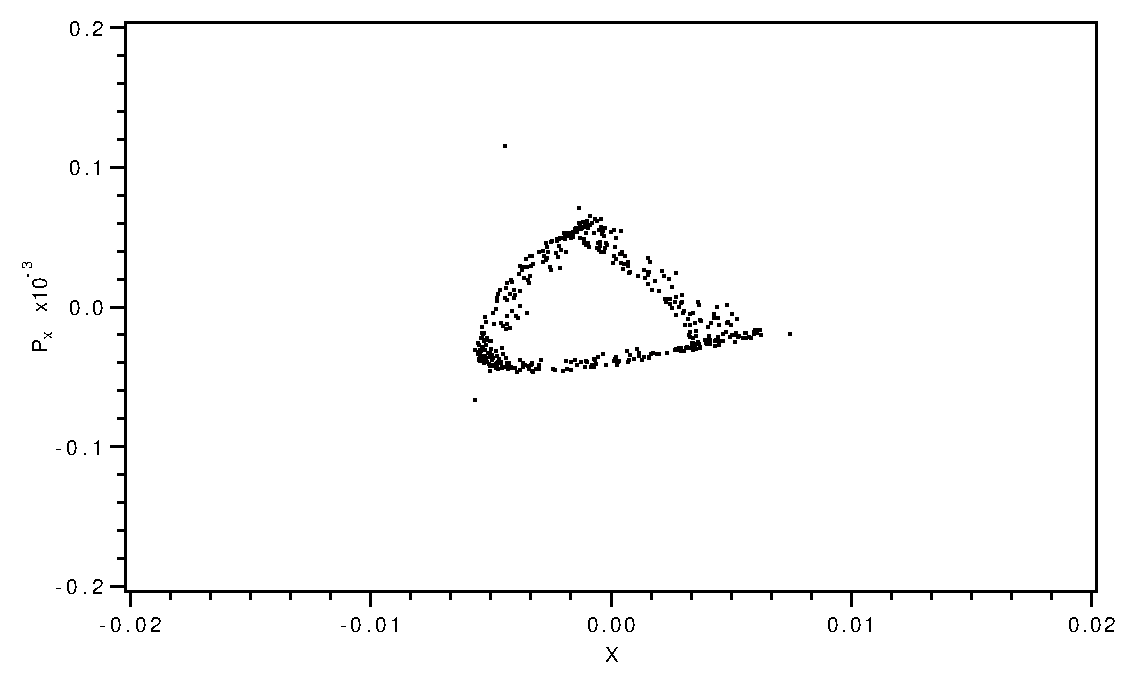
\includegraphics{fig10_13a}
  \caption{Horizontal projection of turn-by-turn phase-space tracking data
(file 14) for lost particle.}
\end{figure}

\newpage
\begin{figure}[htbp]
  \centering
  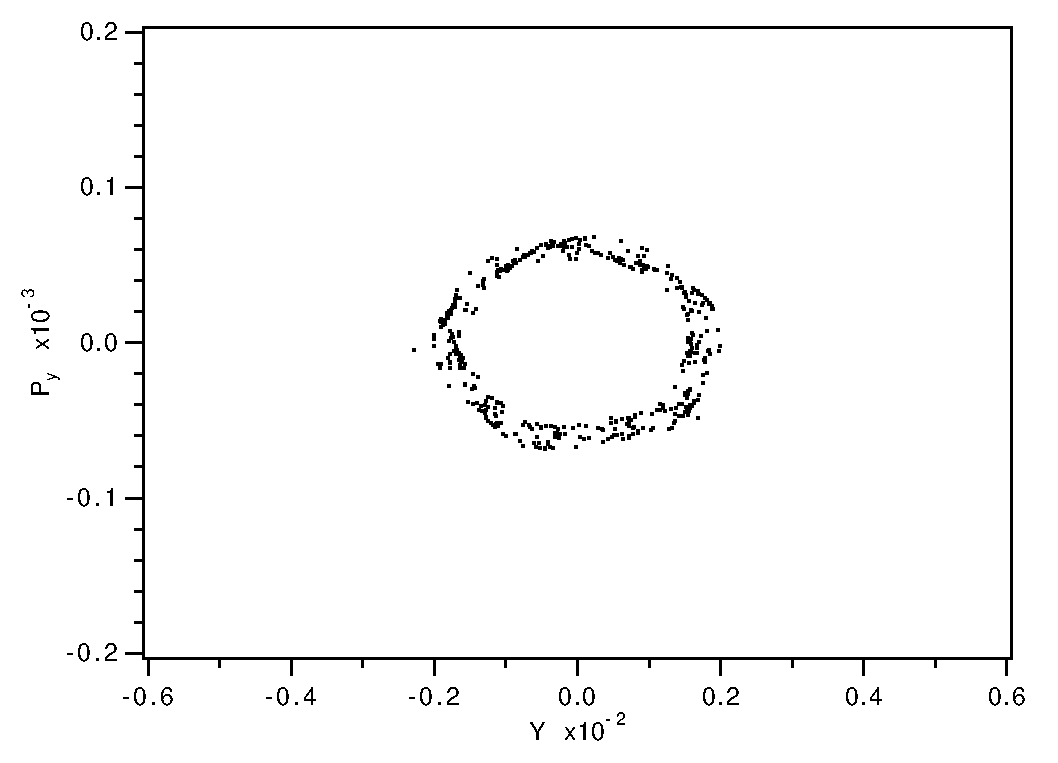
\includegraphics{fig10_13b}
  \caption{Vertical projection of turn-by-turn phase-space tracking data
(file 14) for lost particle.}
\end{figure}

\newpage
\begin{figure}[htbp]
  \centering
  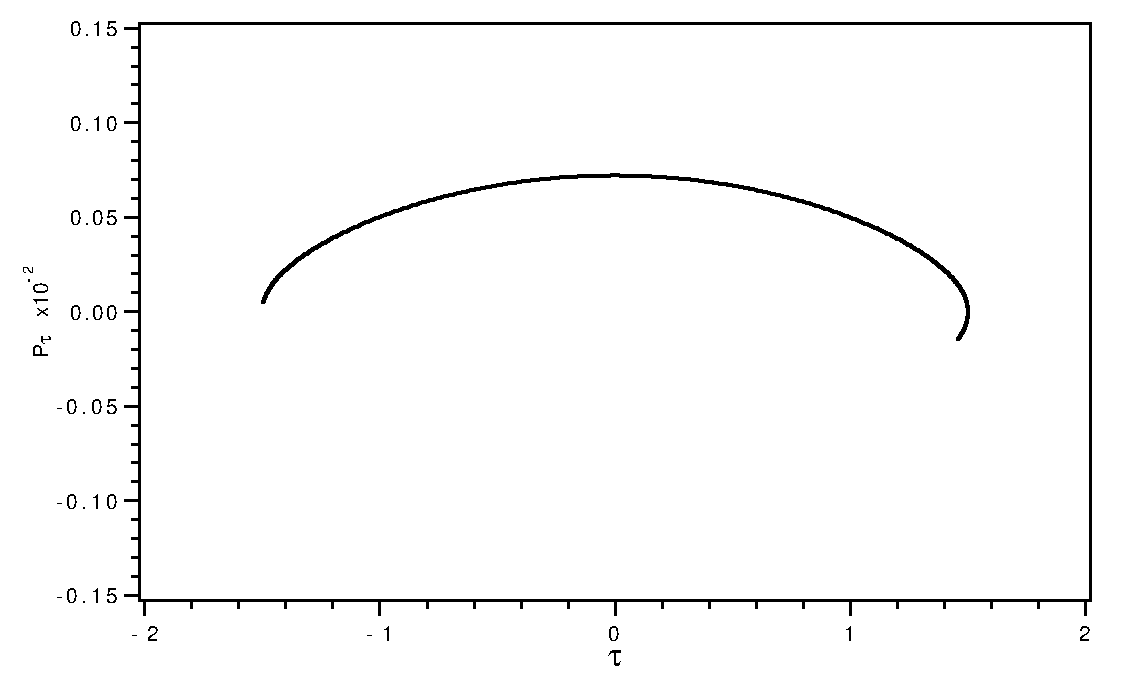
\includegraphics{fig10_13c}
  \caption{Temporal projection of turn-by-turn phase-space tracking data
(file 14) for lost particle.}
\end{figure}

\newpage
\begin{figure}[htbp]
  \centering
  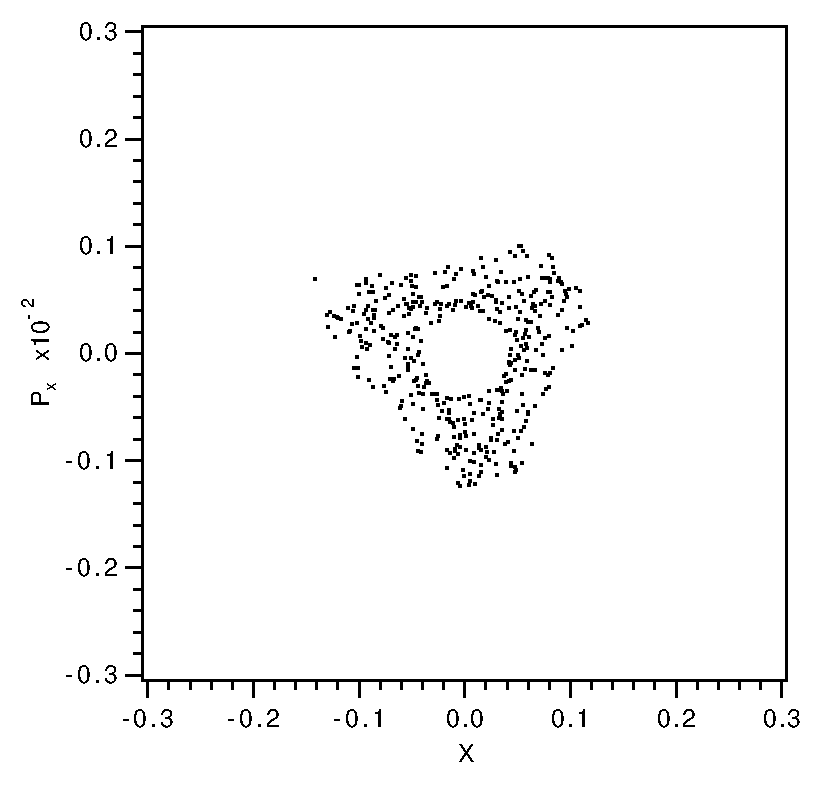
\includegraphics{fig10_14a}
  \caption{Horizontal projection of transformed phase-space data (file 24).}
\end{figure}

\newpage
\begin{figure}[htbp]
  \centering
  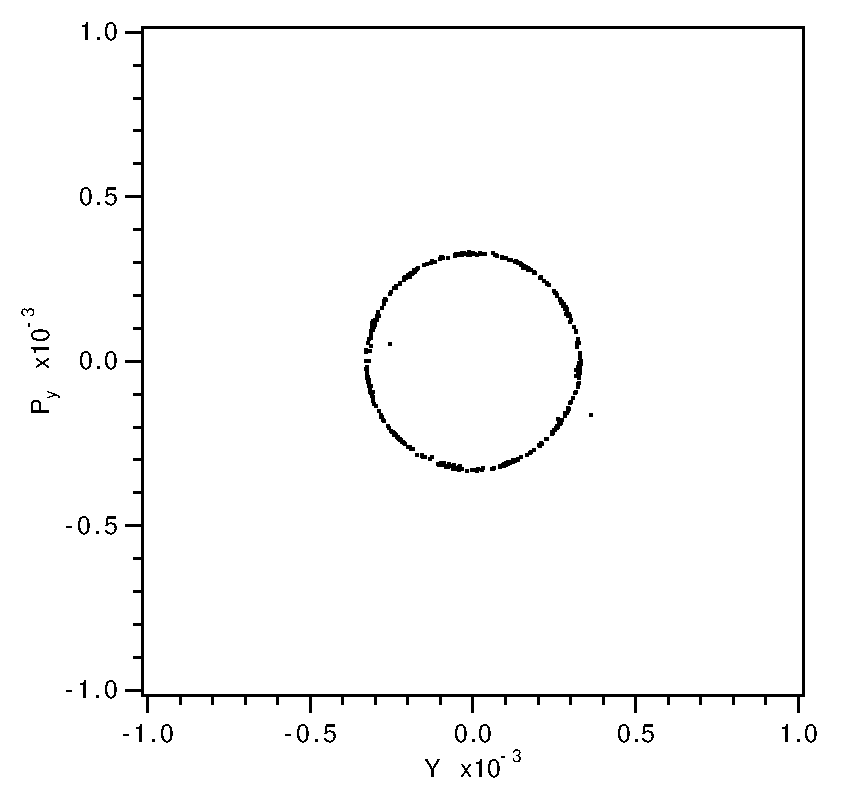
\includegraphics{fig10_14b}
  \caption{Vertical projection of transformed phase-space data (file 24).}
\end{figure}

\newpage
\begin{figure}[htbp]
  \centering
  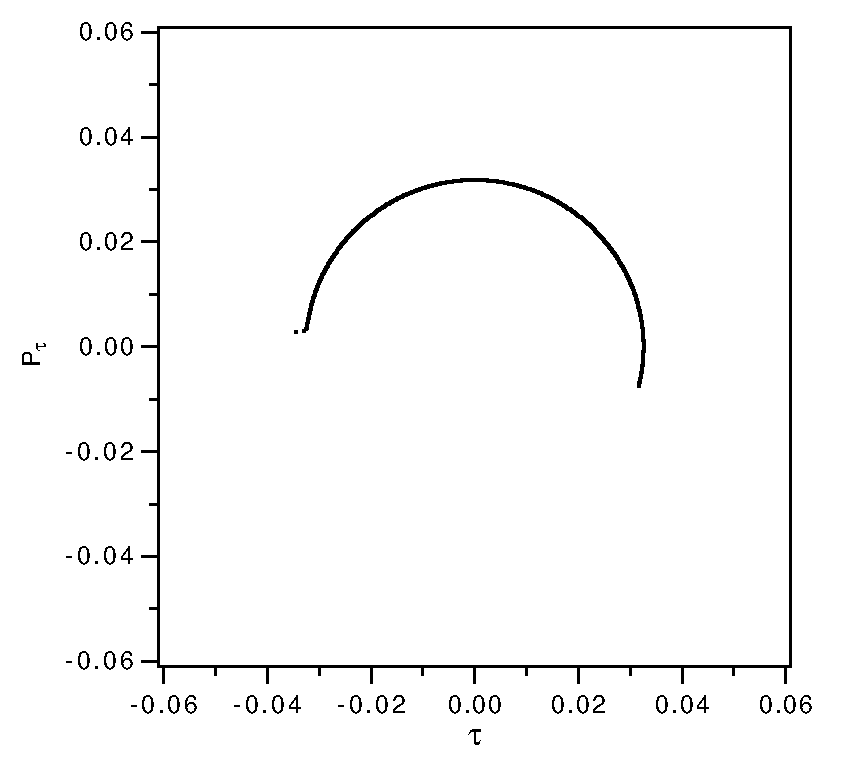
\includegraphics{fig10_14c}
  \caption{Temporal projection of transformed phase-space data (file 24).}
\end{figure}

\begin{footnotesize}
\begin{verbatim}
Exhibit 10.8.2a
First 10 lines from "ordinary" precision initial conditions file
(file 16) produced by the MaryLie run of subsection 10.8.1:

-2.72488E-03  2.24632E-05 -1.12649E-03 -4.52098E-05 -1.33566E+00  3.52445E-04
-2.21313E-03  1.37555E-06 -9.51780E-04  5.21177E-05  1.19509E+00 -4.80832E-04
 1.52671E-03 -1.46330E-05 -1.04655E-03 -4.75277E-05 -4.90794E-01  7.65706E-04
-1.42592E-03  1.59351E-05 -1.26283E-03  4.34335E-05 -2.38677E-01 -7.99465E-04
-1.62590E-03 -3.65853E-05 -2.60833E-04 -5.99301E-05  1.21025E+00  4.64431E-04
 1.10064E-03 -3.00936E-05 -1.24754E-03 -4.11328E-05  1.45749E+00 -1.45480E-04
 4.02458E-03 -9.72345E-06 -1.21551E-03 -4.22860E-05  1.14555E+00 -5.15828E-04
 6.26568E-04  3.84789E-05  1.42061E-03 -3.69284E-05  1.94167E-01 -8.03939E-04
 3.24966E-03 -6.99122E-06  1.70503E-03 -1.46624E-05  1.47949E+00 -3.33364E-05
 3.27788E-03  3.22586E-05 -5.60920E-05  6.09446E-05 -9.70909E-01 -6.09945E-04


Exhibit 10.8.2b
Full precision initial conditions for the lost particle, corresponding to
line 6 above, as extracted from file 18:

 1.100643642212187E-003
-3.009364428172349E-005
-1.247535309762509E-003
-4.113280353188271E-005
  1.45749101315727
-1.454801593473802E-004


Exhibit 10.8.2c
***MARYLIE 3.0***
Prerelease Development Version 8/21/98
Copyright 1987 Alex J. Dragt
All rights reserved

Data input complete; going into #labor.
#comment
Exhibit 10.8.2.
    This is a MARYLIE run to study the dynamic aperture of the Tevatron when
16 distortion sextupoles are powered.  The 'quads' q0c1 and q0c2 are set to
achieve horizontal and vertical tunes of .39 and .46, respectively, and the
'sextupoles' s0c1 and s0c2 are set to achieve zero first-order chromaticities.
Both these fits were made with the RF cavity (rfca) turned off.  In this run
the RF cavity is powered.  As one can see from the response to the tadm
command, the transverse tunes shift slightly when the cavity is turned on due
both to synchro-betatron coupling and the defocussing effects of the cavity.
The distortion sextupoles dsex+ and dsex- are set to strengths corresponding
to 30 amperes  excitation current.  Fringe-field effects are included.
Finally, the beam parameters are those for 150 GeV protons.

This MaryLie run does 10 things:

 a) It computes maps for the lines cxfd and cxdf, which occur
    repeatedly in the Tevatron lattice, and stores them as lumps
    in order to speed up subsequent computations.

 b) It computes 17 transfer maps and writes them out sequentially on file 10.
    The 1st transfer map describes the elements stretching from the location
    of a  horizontal beam position monitor in sector E (location e24) to the
    trailing end of the 1st distortion sextupole.  The 2nd transfer map
    describes the elements from the trailing end of the 1st distortion
    sextupole location to the trailing end of the 2nd distortion
    sextupole. ... The 16th transfer map describes the elements from the
    trailing end of the 15th distortion sextupole location to the trailing
    end of the 16th distortion sextupole.  Finally, the 17th transfer map
    describes the elements from the trailing end of the 16th distortion
    sextupole location back to the horizontal position monitor location.
    Thus, when combined, these 17 transfer maps give a full one-turn map.

 c) It reads these maps back in and stores them as lumps.

 d) These 17 maps are concatenated to give a one-turn map.

 e) A tadm command is used to compute script A and the tunes
    for the one-turn map.

 f) A "lost" linearly matched ray is read in from file 13.

 g) This ray is tracked lump-by-lump, with results written
    on file 14 every turn, until it is lost.

 h) The istat and ihist arrays are written on files 20 and 22,
    respectively.

 i) File 14 is read back in.

 j) The full script A for the one-turn map is gotten from
    buffer 2, inverted, and applied to the tracked rays with
    the results written on file 24.


#beam

***********************************************************
* The #beam, #menu, #lines, #lumps, and #loops components *
* of this file are the same as those in Exhibit 10.8.1c.  *
***********************************************************

#labor
    1*fileout
    1*zer
    1*lcxfd
    1*lcxdf
    1*clear
    1*wring
    1*totmap
    1*tadm
    1*clear
    1*icin
    1*xform14
    1*lmpbylmp
    1*circ14e
    1*stat
    1*hist
    1*clear
    1*raysin
    1*gbuf2
    1*inv
    1*mapout
    1*xform24
    1*end

*********************************************************
* The responses to the #labor entries 1*fileout, 1*zer, *
* 1*lcxfd, 1*lcxdf, 1*clear, 1*wring, 1*totmap, 1*tadm, *
* and 1*clear are the same as in Exhibit 10.8.1c.       *
*********************************************************

*********************************
* Response to the icin command: *
*********************************

    1 ray(s) read in from file  13

***************************************
* Response to the circ command, etc.: *
***************************************

circulating through lmpbylmp :
 lm1      lm2      lm3      lm4      lm5
 lm6      lm7      lm8      lm9      lm10
 lm11     lm12     lm13     lm14     lm15
 lm16     lm17

 Search did not converge; root=  0.70331E-01

all particles lost

istat written on file           20
nlost =           1
ihist written on file           22

***********************************
* Response to the raysin command: *
***********************************

  427 ray(s) read in from file  14

******************************************
* The transforming map script A inverse: *
******************************************

matrix for map is :

 9.96432E-02  0.00000E+00 -3.85387E-21 -6.00495E-20  6.31758E-07  2.17124E-01
-1.40221E-04  1.00358E+01  5.66633E-22  4.36877E-20  3.45704E-07  9.96505E-02
-7.24095E-17  6.17887E-14  1.86914E-01  0.00000E+00  3.03092E-17 -2.19142E-16
-2.87319E-17 -6.80430E-14  6.08481E-03  5.35004E+00  1.76267E-20 -5.46098E-16
-2.33048E-04  5.09857E-02 -3.28674E-18  4.19422E-18  2.33986E-02  0.00000E+00
 6.08413E-07 -8.11623E-05  2.48534E-19  1.86323E-17  8.71051E-05  4.27377E+01

nonzero elements in generating polynomial are :

 f( 28)=f( 30 00 00 )=  110.33115619351
 f( 29)=f( 21 00 00 )=  230.08011452766
 f( 32)=f( 20 00 10 )=-7.64236363671544E-04
 f( 33)=f( 20 00 01 )= 0.21061201497236
 f( 34)=f( 12 00 00 )= -409.33709895966
 f( 37)=f( 11 00 10 )=-1.98308774624551E-02
 f( 38)=f( 11 00 01 )= -1.5346294736954
 f( 39)=f( 10 20 00 )= -50.321815269185
 f( 40)=f( 10 11 00 )= -112.64954194020
 f( 43)=f( 10 02 00 )=  67.674674230258
 f( 46)=f( 10 00 20 )= 5.49264263214689E-07
 f( 47)=f( 10 00 11 )=-4.22537781016221E-05
 f( 48)=f( 10 00 02 )=-1.16100284894868E-02
 f( 49)=f( 03 00 00 )= -41.301620516121
 f( 52)=f( 02 00 10 )=-6.25872941601144E-04
 f( 53)=f( 02 00 01 )= 0.28339015039882
 f( 54)=f( 01 20 00 )= -53.913467515215
 f( 55)=f( 01 11 00 )=  145.98463472258
 f( 58)=f( 01 02 00 )=  18.416597618544
 f( 61)=f( 01 00 20 )=-2.43635493527592E-07
 f( 62)=f( 01 00 11 )=-2.47356004995205E-05
 f( 63)=f( 01 00 02 )= 1.05531720326059E-02
 f( 66)=f( 00 20 10 )=-1.44291715055299E-03
 f( 67)=f( 00 20 01 )=-0.14964403783604
 f( 69)=f( 00 11 10 )= 1.95582556852843E-02
 f( 70)=f( 00 11 01 )= 0.33591713531964
 f( 75)=f( 00 02 10 )= 1.38441203994220E-03
 f( 76)=f( 00 02 01 )= 0.18024669588979
 f( 80)=f( 00 00 30 )=-7.22824267157899E-03
 f( 81)=f( 00 00 21 )=-9.73630888091078E-10
 f( 82)=f( 00 00 12 )=-1.08424609271605E-02
 f( 83)=f( 00 00 03 )= 3.30917571378989E-05
 f( 84)=f( 40 00 00 )= -3699.1440602575
 f( 85)=f( 31 00 00 )=  42321.968671425
 f( 86)=f( 30 10 00 )= 2.66770915391513E-09
 f( 87)=f( 30 01 00 )=-2.33112222830107E-09
 f( 88)=f( 30 00 10 )=  4.5693950614251
 f( 89)=f( 30 00 01 )=  482.31125364226
 f( 90)=f( 22 00 00 )= -28181.836095754
 f( 91)=f( 21 10 00 )= 4.69209955695986E-09
 f( 92)=f( 21 01 00 )= 2.86314136454196E-09
 f( 93)=f( 21 00 10 )=  2.8759571796469
 f( 94)=f( 21 00 01 )= -429.63407177763
 f( 95)=f( 20 20 00 )=  12568.221040625
 f( 96)=f( 20 11 00 )= -209898.00228013
 f( 99)=f( 20 02 00 )= -7762.0900789243
 f(100)=f( 20 01 10 )=-2.38388163473635E-10
 f(102)=f( 20 00 20 )= -2.0075663524607
 f(103)=f( 20 00 11 )= -2075.1974330970
 f(104)=f( 20 00 02 )=-0.84614616589268
 f(105)=f( 13 00 00 )= -39644.566479127
 f(106)=f( 12 10 00 )= 5.32303330736889E-09
 f(107)=f( 12 01 00 )= 2.99482383271274E-10
 f(108)=f( 12 00 10 )=  5.1084562336192
 f(109)=f( 12 00 01 )=  236.07859432082
 f(110)=f( 11 20 00 )=  195669.82408561
 f(111)=f( 11 11 00 )=  51210.427258493
 f(112)=f( 11 10 10 )= 4.56259809595747E-10
 f(114)=f( 11 02 00 )= -194877.67131442
 f(117)=f( 11 00 20 )=-1.72811708277018E-02
 f(118)=f( 11 00 11 )= 7.12792983006422E-02
 f(119)=f( 11 00 02 )=  2.1815181618326
 f(120)=f( 10 30 00 )= 8.35080084371653E-09
 f(121)=f( 10 21 00 )=-2.27815722867953E-08
 f(122)=f( 10 20 10 )= -1.0536861517615
 f(123)=f( 10 20 01 )= -104.83855687539
 f(124)=f( 10 12 00 )=-1.45097237919057E-08
 f(125)=f( 10 11 10 )=-0.30587522080300
 f(126)=f( 10 11 01 )= -31.943377023477
 f(130)=f( 10 03 00 )= 1.01799936033082E-08
 f(131)=f( 10 02 10 )=  2.1028938077905
 f(132)=f( 10 02 01 )=  272.62188535886
 f(136)=f( 10 00 30 )=-5.55035395974697E-03
 f(137)=f( 10 00 21 )=-2.54193944373808E-04
 f(138)=f( 10 00 12 )=-1.43680084374256E-03
 f(139)=f( 10 00 03 )=-0.10479626465914
 f(140)=f( 04 00 00 )=  13093.089425509
 f(141)=f( 03 10 00 )= 4.89253100381726E-09
 f(142)=f( 03 01 00 )= 6.66471433660047E-09
 f(143)=f( 03 00 10 )= 0.35229448191160
 f(144)=f( 03 00 01 )=  330.76671162514
 f(145)=f( 02 20 00 )= -12389.381627853
 f(146)=f( 02 11 00 )=  212861.34726061
 f(149)=f( 02 02 00 )=  7583.2506661522
 f(150)=f( 02 01 10 )= 2.54415888439787E-10
 f(152)=f( 02 00 20 )= -2.0076971688682
 f(153)=f( 02 00 11 )= -2075.2312117017
 f(154)=f( 02 00 02 )=  4.8614096872223
 f(155)=f( 01 30 00 )= 7.40792041676429E-09
 f(156)=f( 01 21 00 )= 2.05883291330874E-08
 f(157)=f( 01 20 10 )=-0.53529042536235
 f(158)=f( 01 20 01 )=  93.904554169546
 f(159)=f( 01 12 00 )=-2.61215632847230E-08
 f(160)=f( 01 11 10 )= -3.6720314500957
 f(161)=f( 01 11 01 )= -212.26272557163
 f(165)=f( 01 03 00 )=-2.83383161190976E-09
 f(166)=f( 01 02 10 )= 0.15940346968810
 f(167)=f( 01 02 01 )= -38.870700999373
 f(171)=f( 01 00 30 )= 1.01415279468839E-02
 f(172)=f( 01 00 21 )= 3.68071933105609E-04
 f(173)=f( 01 00 12 )=-6.65930436712669E-04
 f(174)=f( 01 00 03 )=-2.13851125596395E-02
 f(175)=f( 00 40 00 )=  1764.2193369969
 f(176)=f( 00 31 00 )=  9514.4347875228
 f(179)=f( 00 22 00 )= -6227.0170299587
 f(182)=f( 00 20 20 )= 0.11708889760202
 f(183)=f( 00 20 11 )= -1.7999560071408
 f(184)=f( 00 20 02 )=-0.22321197489726
 f(185)=f( 00 13 00 )= -6956.9519944126
 f(188)=f( 00 11 20 )= 3.68164741059018E-03
 f(189)=f( 00 11 11 )= 2.29356563091016E-02
 f(190)=f( 00 11 02 )=  1.1225239665317
 f(195)=f( 00 04 00 )=  311.45300632266
 f(198)=f( 00 02 20 )= 0.12041502369326
 f(199)=f( 00 02 11 )= -1.8120938764225
 f(200)=f( 00 02 02 )=-1.42919463980606E-02
 f(205)=f( 00 00 40 )=-0.21862430319272
 f(206)=f( 00 00 31 )=  58.625111502592
 f(207)=f( 00 00 22 )= 0.26191390160400
 f(208)=f( 00 00 13 )=  35.107274558903
 f(209)=f( 00 00 04 )= 0.13131966932472

end of MARYLIE run
\end{verbatim}
\end{footnotesize}

\section{Production of Lattice Function Plots}\index{plots} \index{lattice function plots}
\label{prodlatt}
The production of lattice function plots requires 4 steps:
\begin{enumerate}
\item Specifying at what locations the lattice functions are to be
calculated.
\item Calculating various geometric properties of the lattice, such as
path length, at these locations and arranging to have these quantities
written out onto a file.
\item Arranging to have the lattice functions calculated at these
same locations and the desired results written out onto the same file.
\item Using the file generated in steps 2 and 3 above to
produce lattice function plots.
\end{enumerate}
These steps will be illustrated in this section for the case of the
Proton Storage Ring example described previously in section 2.5.

Step 1 is most easily made in the case that lattice functions are to be
computed only at locations between successive elements.  If lattice
functions are desired with finer spacing along the lattice, it is
necessary to split elements.  To illustrate element splitting, this
example splits dipoles and long and medium-long drifts into 5 pieces, and
quadrupoles and sextupoles in two.  Splitting parallel faced
(rectangular) bends is the most complicated operation.  Here use is made
of the factorization of section 6.6 that employs incoming and outgoing maps
surrounding a normal entry (sector) bend.  The normal entry bend in turn
is easily split into any number (5 in this case) of wedges. \index{slicing elements} \index{splitting elements}

Compare Exhibit 2.5a in section 2.5 with the Master Input File of this
section, Exhibit 10.9c.  In Exhibit 10.9c the menu entries {\em drml,
drl, bend, hfq}, and {\em hdq} found in Exhibit 2.5a are replaced with
the entries {\em cdrml, cdrl, cbend, chfq}, and {\em chdq}, respectively,
where the prefix letter {\em c} stands for {\em complete}.  Inspection of the
rest of the Master Input File in Exhibit 10.9c shows that the
``complete'' menu entries are not actually used.  They merely serve as a
reminder of things past and a resource for future use.  Instead, as can
be verified by inspection, the original menu entries {\em drml, drl,
$\cdots$ hfq, hdq} now appear as {\em lines} in the {\em \#lines}
component of the Master Input File.  The contents of these lines in turn
contain new menu entries.  For example, the line {\em drml} is defined by
the statement:

\begin{footnotesize}
\begin{verbatim}
 drml
     5*drml/5
\end{verbatim}
\end{footnotesize}
Reference to the {\em \#menu} component shows that {\em drml/5} is a drift
whose length is 1/5 that of the original medium-long drift {\em drml}.
Thus, the medium-long drift has been split into 5 pieces.  Similarly, the
sextupoles {\em hcs} and {\em vcs} have each been split into two pieces.

As mentioned earlier, splitting of the bend is somewhat more involved.
Inspection of the line {\em bend} shows that it has the contents:

\begin{footnotesize}
\begin{verbatim}
 bend
     1*inprot      1*infrng      1*ingbdy      5*sbend/5     1*outgbdy  &
     1*outfrng     1*outprot
\end{verbatim}
\end{footnotesize}
Reference to {\em \#menu} shows that {\em sbend/5} is a normal entry (sector)
bend whose angle is 1/5 that of the original bend.  Thus, in view of the
factorization described in Exhibit 6.6.1, the bend has also been split
into 5 pieces.

Finally, the quadrupoles have been split into leading and trailing
halves.  For example, the horizontal focusing quadrupole {\em hfq} is
defined by the statement:

\begin{footnotesize}
\begin{verbatim}
 hfq
     1*inhfq       1*outhfq
\end{verbatim}
\end{footnotesize}
Reference to {\em \#menu} shows that {\em inhfq} is a quadrupole of half
the original length with a leading fringe field but no trailing fringe
field.  Similarly, {\em outhfq} is a half-length quadrupole with no
leading fringe field but a trailing fringe field.  Thus, the horizontal
focusing quadrupole has been split into 2 pieces.

The discussion so far has been devoted to the sometimes necessary, but
still ancillary, subject of splitting elements.  The main subject is how
to specify at what locations in the lattice various functions are to be calculated.
Inspection of the {\em \#lines} components of Exhibits 2.5a and 10.9c
show that they both contain, in identical form, the lines {\em nsex, tsex,
lsex, half}, and {\em ring}.  In addition, Exhibit 10.9c also contains
the lines {\em \%tsex} and {\em \%ring}.  Examination of the contents of
these lines shows that they are ``split'' versions of the lines {\em
tsex} and {\em ring}, respectively, and in addition every entry is
surrounded by the character {\em \%}.  These lines were prepared in a
\Mary run with the help of the {\em wcl} commands {\em wcl10} and {\em
wcl15}.  See the {\em \#menu} component of Exhibit 10.9c and section
7.33.  Observe that the {\em \#loops} component of Exhibit 10.9c contains
the loops {\em ltsex} and {\em lring}.  Suppose these loops are invoked
in turn in {\em \#labor} followed by the commands {\em wcl15} and {\em
wcl20} as shown below:

\begin{footnotesize}
\begin{verbatim}
#labor
    1*fileout
    1*ltsex
    1*wcl10
    1*lring
    1*wcl15
    1*fin
\end{verbatim}
\end{footnotesize}
Such a \Mary run produces the contents of {\em \%tsex} in file 10 and the
contents of {\em \%ring} in file 15.  These contents can then be copied,
using an editor, into the {\em \#lines} component of a Master Input File
and given the names {\em \%tsex} and {\em \%ring}, as was done to prepare
the Master Input File of Exhibit 10.9c.

What is the point of having the lines {\em \%tsex} and {\em \%ring}?  As
will be seen, they can be used to produce \Mary runs which compute both
lattice functions and geometric quantities at every lattice location
where the symbol {\em \%} appears.  Thus, the line {\em \%ring} can be
used to produce lattice function plots with data points between every
element and within every split element in the entire ring.  Similarly,
the line {\em \%pring}, which contains {\em \%phalf} which in turn
contains {\em \%tsex}, can be used to produce lattice function plots for
only the {\em tsex} portion of half the ring with data points between
every element and within every split element in {\em tsex}..  This
completes the description of step 1.

The next step is to actually arrange to have lattice functions calculated
at each \% location and the desired results written out onto a file.
This can be accomplished by defining a {\em line} whose name is \% and
whose contents specify the work that is to be done.  Suppose, as in this
example, that what is desired are various lattice functions at all the
locations specified by a \% sign.  Then, similar to the case of section
10.5, it is first necessary to do some ``setup'' work in which the total
one-turn map is computed and stored.  This is accomplished by the entries in
the line {\em setup} as shown below:

\begin{footnotesize}
\begin{verbatim}
 setup
     1*iden        1*ring        1*stotmap        1*pli0     1*sq          1*iden
\end{verbatim}
\end{footnotesize}
When {\em setup} is invoked in {\em \#labor}, the entries {\em ring} and
{\em stotmap} result in the computation and storage of the one-turn
total map.  The command {\em pli0} places path-length information in the
fitting array.  (It could have been omitted here.)  In addition and for convenience, {\em setup} also contains
the entry {\em sq} that selects the quantities to be written out.  See
section 8.26.  In this case, {\em sq} receives its instructions from
file 20, whose contents are listed in Exhibit 10.9a.

The stage has now been set to present a description of the contents of the
line {\em \%}.  As can be verified from the {\em \#lines} component of
Exhibit 10.9c, it has the following entries:

\begin{footnotesize}
\begin{verbatim}
 %
     1*pli0        1*work
\end{verbatim}
\end{footnotesize}
The entry {\em pli0} places current path-length information in the
fitting/writing array so that it can be written out subsequently in
response to the {\em wsq} command.  The entry {\em work} is the name of a line that specifies the work to be
done (in this case the computation of lattice functions).

In order to compute a lattice function at some location, it is first
necessary to compute the Poincare surface of section map for this
location.  This is accomplished by the line {\em cpssmap} that appears in
{\em work}:

\begin{footnotesize}
\begin{verbatim}
 work
     1*cpssmap     1*anal        1*wsq         1*restore
\end{verbatim}
\end{footnotesize}
As can be seen, the entries in {\em cpssmap} result in storing the
current map ({\em scurmap}), inverting it ({\em inv}), concatenating the
result with the total map ({\em gtotmap}), and concatenating that result with
the current map ({\em gcurmap}):

\begin{footnotesize}
\begin{verbatim}
cpssmap
     1*scurmap     1*inv         1*gtotmap     1*gcurmap
\end{verbatim}
\end{footnotesize}
That is, as in the example of section 10.5, there is the product relation
\begin{center}
current Poincare surface of section map = \\
(current accumulated  map)$^{-1}$ (total map) (current accumulated map).
\end{center}

Once the current Poincare surface of section map has become available, it
is analyzed using the command in the line {\em anal}, in this case a
silent {\em tasm} command (and a {\em snor} command whose purpose will be
described later):

\begin{footnotesize}
\begin{verbatim}
anal
     1*stasm       1*snor
\end{verbatim}
\end{footnotesize}
See the contents of {\em work} and section 8.2.  Next, those results of
{\em pli0} and {\em anal} ({\em tasm} in this case) previously selected by {\em sq} are
written to an external file using the {\em wsq} command.  See section
8.27.  Finally, again see the contents of {\em work}, the line {\em
restore} makes the accumulated map the current map:

\begin{footnotesize}
\begin{verbatim}
restore
     1*iden        1*gcurmap
\end{verbatim}
\end{footnotesize}
Steps 2 and 3 have now been accomplished.  For example, if the lines {\em setup}
and {\em \%ring} are invoked in {\em \#labor} (see the {\em \#labor}
component of Exhibit 10.9e), then at each lattice location in {\em \%ring}
marked by a \% sign the path-length information and lattice functions specified by {\em sq} are
written to an external file, in this case file 30.  See Exhibit 10.9b.

Step 4 is accomplished by processing file 30 with some plotting program to produce
various lattice function plots.  Figures 9.1 through 9.4 show plots around
the ring of the first-order horizontal dispersion functions {\em dz1} and
{\em dz2} and the
horizontal and vertical beta functions.

Sometimes it may be desirable to have lattice function plots for only
some selected part of the lattice.  This is also easily done.  For
example, suppose a lattice function plot is desired only for a {\em tsex}
portion of the ring.  This can be accomplished by replacing (in {\em \#labor})
{\em \%ring} with {\em \%pring}.  Figures 9.5 and 9.6 show, for example, plots of the
first-order dispersion functions for just the final {\em tsex} portion of
the ring.

In the examples presented so far all the lattice functions have been the
usual {\em linear} lattice functions.  \Mary can
also compute and produce {\em nonlinear} lattice functions.  All lattice
functions are various entries in or functions of the entries in the transforming map ${\cal A}$.  This
map is available through the commands {\em snor} and {\em dnor}.  See
sections 8.8 and 8.9.  Now it can be understood why in this example a {\em snor} command
is also part of the {\em anal} line and why, to illustrate the case of a
nonlinear lattice function, the {\em sq} command has been instructed to
select also the f(28) entry in ${\cal A}$ (available in buffer 1).  This
entry is
the coefficient of the {\em X$^3$} generator.  See sections 8.8 and 14.1 and
Exhibit 10.9a.  Figure 9.7 shows this nonlinear lattice function for the final {\em
tsex} portion of the ring.

Upon examining figures 9.1, 9.2, 9.3, 9.5, 9.6, and 9.7, the reader might
wonder about the origin of what appear to be anomalous spikes.  They are
an artifact of the splitting process for dipoles.  See section 10.13.1
for further explanation and how they can be avoided.

\newpage
\begin{figure}[htbp]
\renewcommand{\thefigure}{\thesection.\arabic{figure}}
  \centering
  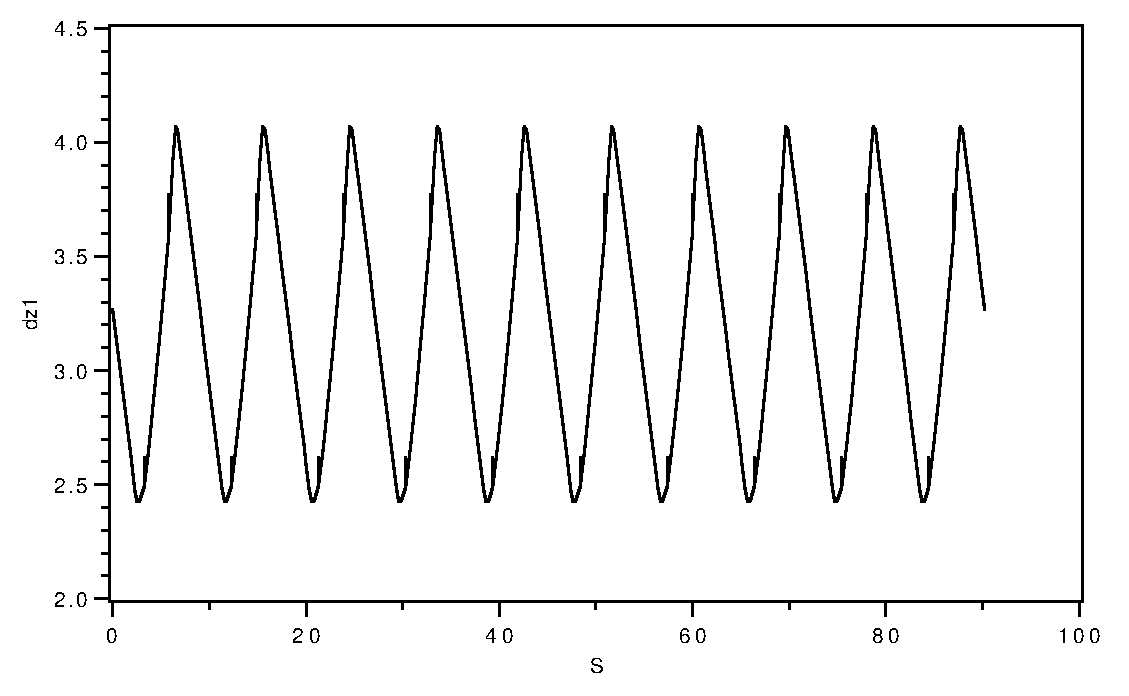
\includegraphics{fig10_15a}
  \caption{Plot of the first-order ``X'' dispersion function {\em dz1} for the
entire ring.}
\end{figure}

\newpage
\begin{figure}[htbp]
\renewcommand{\thefigure}{\thesection.\arabic{figure}}
  \centering
  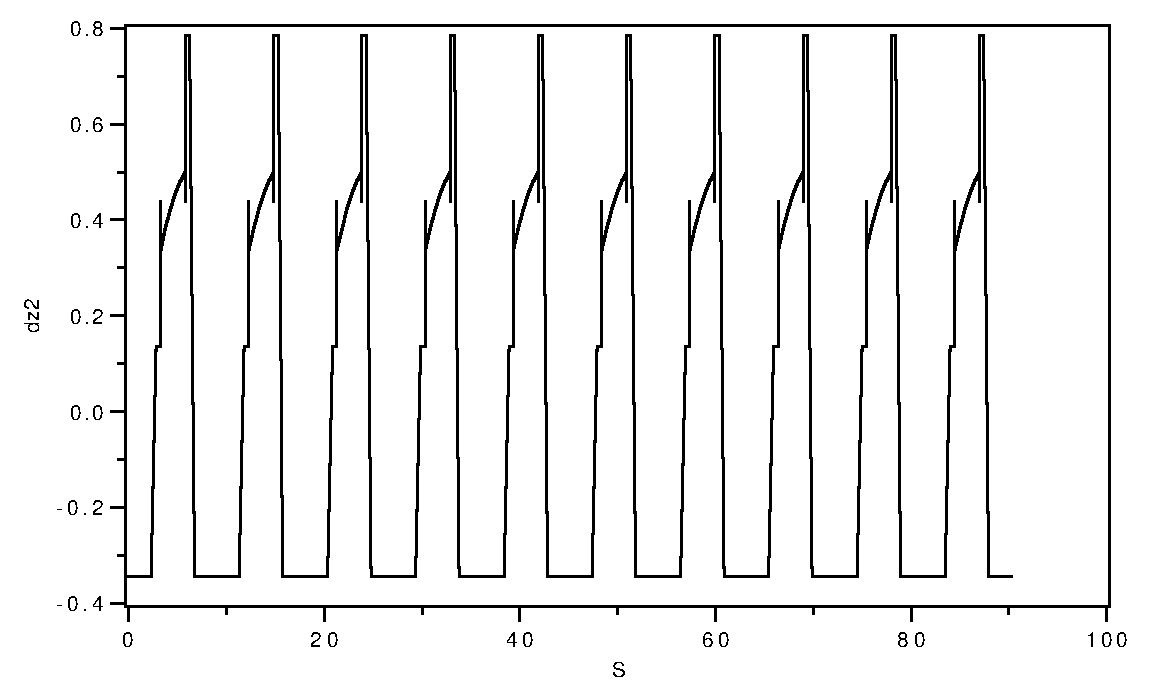
\includegraphics{fig10_15b}
  \caption{Plot of the first-order ``P$_x$'' dispersion function {\em dz2} for the
entire ring.}
\end{figure}

\newpage
\begin{figure}[htbp]
\renewcommand{\thefigure}{\thesection.\arabic{figure}}
  \centering
  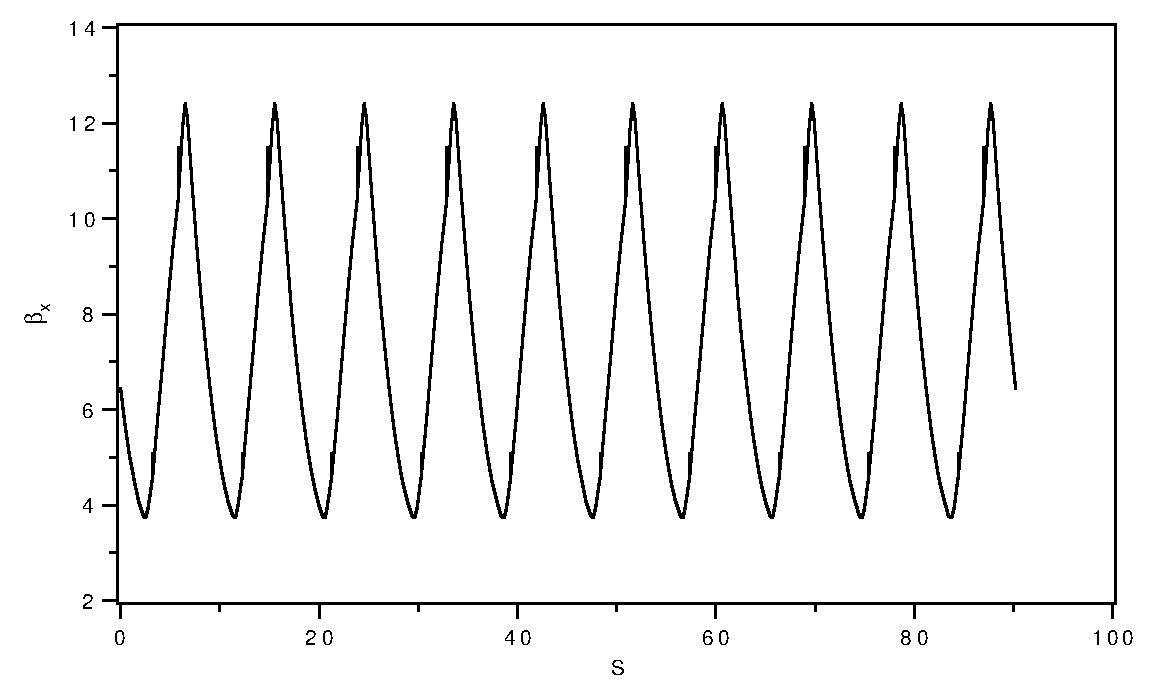
\includegraphics{fig10_15c}
  \caption{Plot of the horizontal beta function {\em bx} for the
entire ring.}
\end{figure}

\newpage
\begin{figure}[htbp]
\renewcommand{\thefigure}{\thesection.\arabic{figure}}
  \centering
  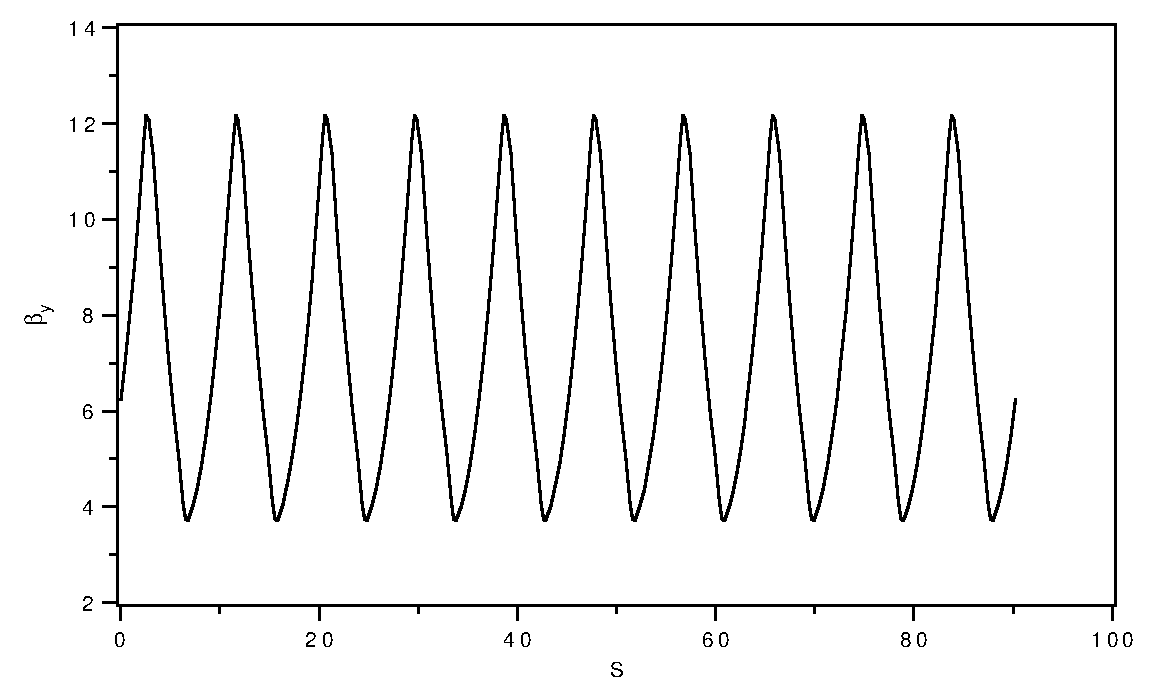
\includegraphics{fig10_15d}
  \caption{Plot of the vertical beta function {\em by} for the
entire ring.}
\end{figure}

\newpage
\begin{figure}[htbp]
\renewcommand{\thefigure}{\thesection.\arabic{figure}}
  \centering
  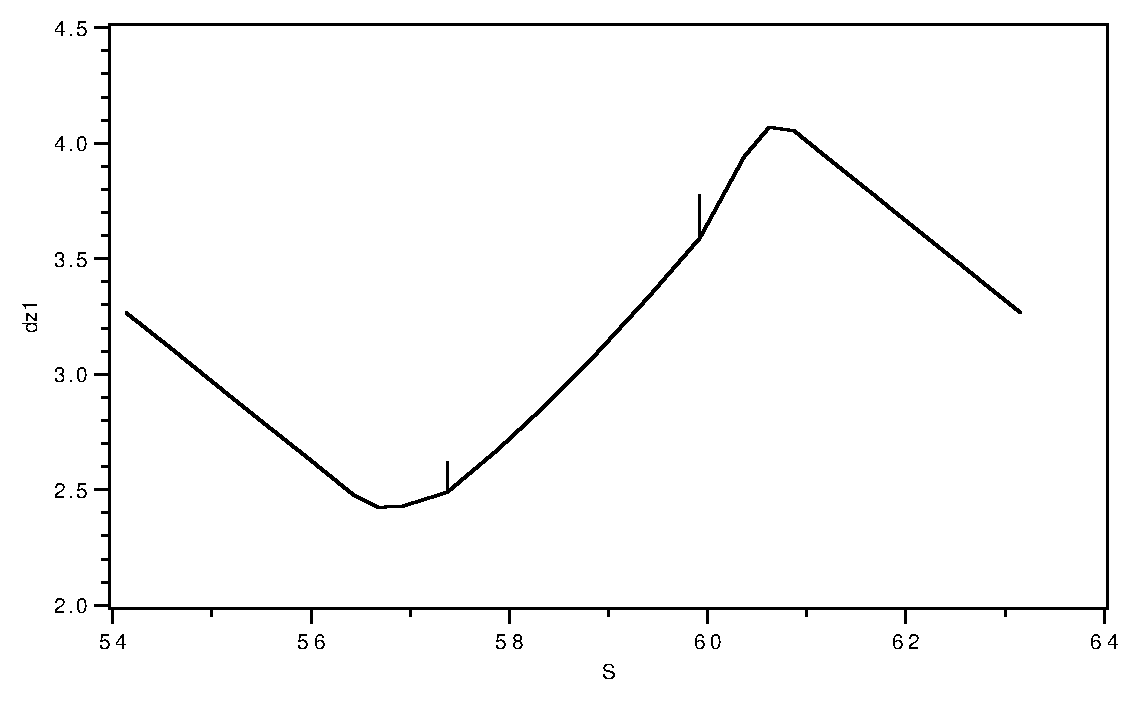
\includegraphics{fig10_16a}
  \caption{Plot of the first-order ``X'' dispersion function {\em dz1} for the
final {\em tsex} portion of the ring.}
\end{figure}

\newpage
\begin{figure}[htbp]
\renewcommand{\thefigure}{\thesection.\arabic{figure}}
  \centering
  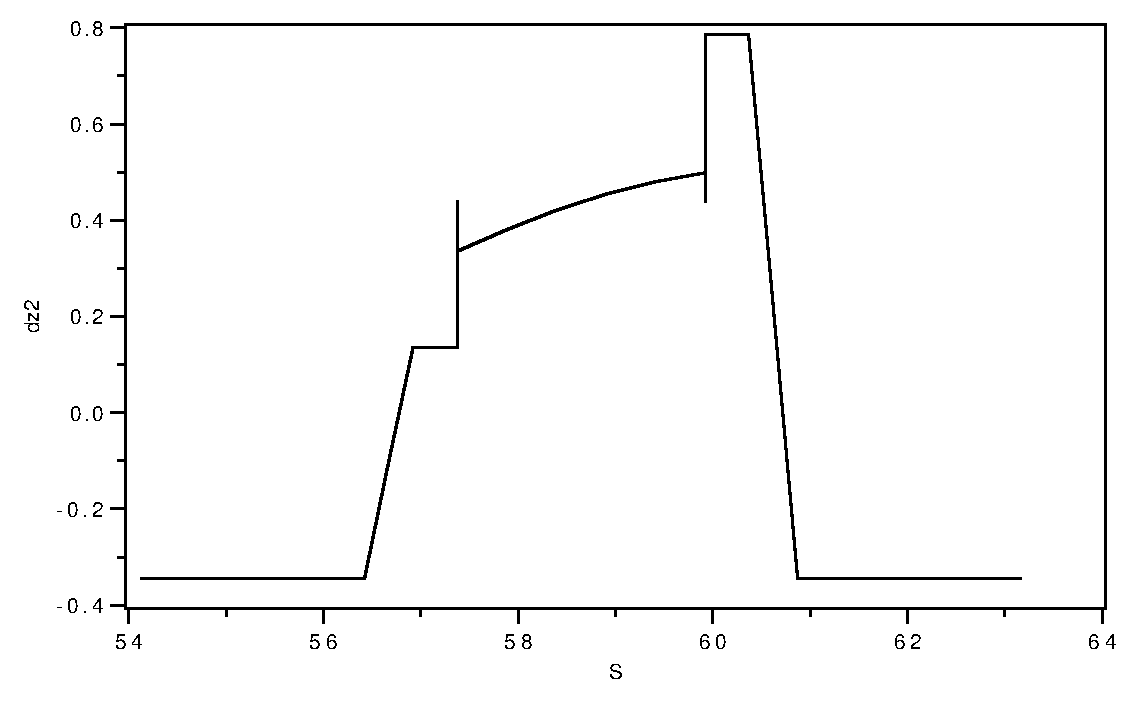
\includegraphics{fig10_16b}
  \caption{Plot of the first-order ``P$_x$'' dispersion function {\em dz2} for the
final {\em tsex} portion of the ring.}
\end{figure}

\newpage
\begin{figure}[htbp]
\renewcommand{\thefigure}{\thesection.\arabic{figure}}
  \centering
  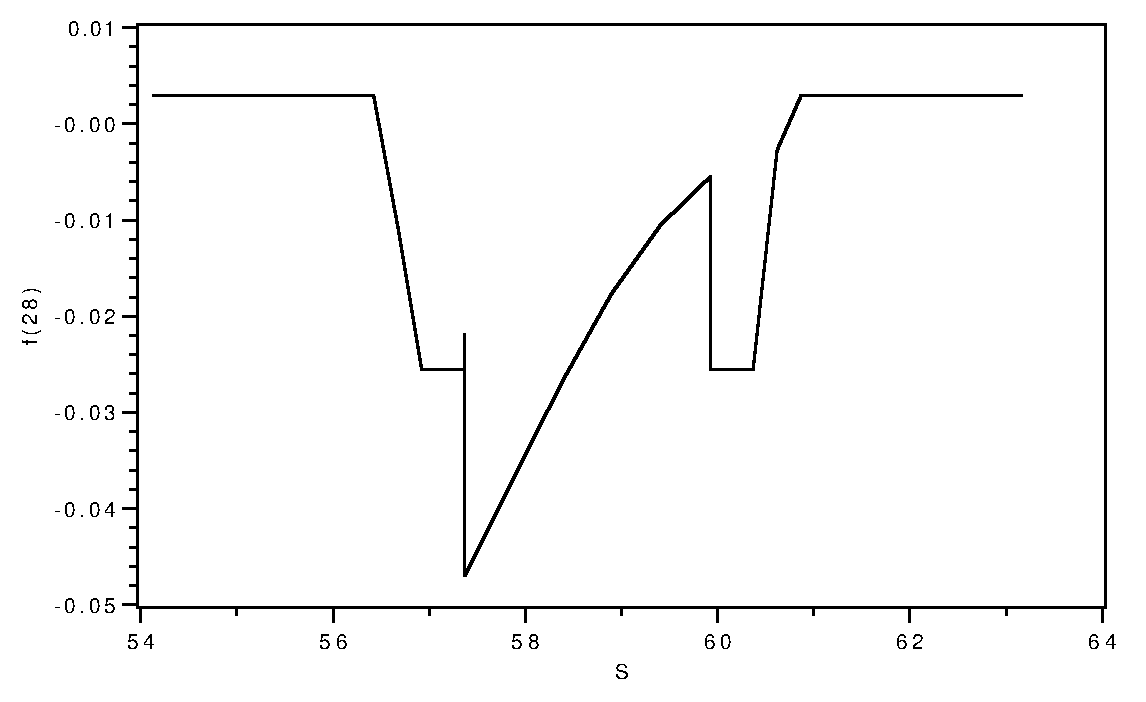
\includegraphics{fig10_16c}
  \caption{Plot, for the final {\em tsex} portion of the ring, of the nonlinear lattice function that is the coefficient of the
$X^3$ generator in ${\cal A}$.}
\end{figure}

\newpage
\begin{footnotesize}
\begin{verbatim}
Exhibit 10.9a
Instructions in file 20 for the sq command:

 1  bf1( 28)
 2       dz1
 3       dz2
 4        bx
 5        by
 6        pl
 #


Exhibit 10.9b
First few lines of file 30 written as a result of the wsq command.
In agreement with Exhibit 10.9a above, the columns are bf1(28),
dz1, dz2, bx, by, and pl, respectively:

  2.97958E-03  3.26669E+00 -3.44101E-01  6.43759E+00  6.23191E+00  0.00000E+00
  2.97958E-03  3.10933E+00 -3.44101E-01  5.66815E+00  7.08761E+00  4.57292E-01
  2.97958E-03  2.95198E+00 -3.44101E-01  5.01700E+00  8.06134E+00  9.14584E-01
  2.97958E-03  2.79462E+00 -3.44101E-01  4.48413E+00  9.15310E+00  1.37188E+00
  2.97958E-03  2.63727E+00 -3.44101E-01  4.06956E+00  1.03629E+01  1.82917E+00
  2.97958E-03  2.47991E+00 -3.44101E-01  3.77328E+00  1.16907E+01  2.28646E+00
 -1.05970E-02  2.42416E+00 -1.02875E-01  3.75309E+00  1.21683E+01  2.53646E+00
 -2.54879E-02  2.42827E+00  1.35811E-01  3.95404E+00  1.20626E+01  2.78646E+00

Exhibit 10.9c
***MARYLIE 3.0***
Prerelease Development Version 6/17/99
Copyright 1987 Alex J. Dragt
All rights reserved

Data input complete; going into #labor.
#comment
 Exhibit 10.9
      This is a MaryLie run that employs the pli and other type codes to
 produce lattice function plot data using the PSR as an example.  The
 dipoles and the long and medium-long drifts are split into 5 pieces.
 Quads and sextupoles are split in two.  This run generates lattice function
 plot data for the entire ring.  If the "labor" component is modified to
 take the form shown below, the run will generate lattice function plot
 data for just the final tsex portion of the ring:

 labor
   fileout
   setup
   %pring
   fin

#beam
  4.86914813175970
 0.849425847892200
  1.00000000000000
  1.00000000000000
#menu
 pli0     pli
  0.000000000000000E+00
 drvs     drft
  0.300000000000000
 drs      drft
  0.450000000000000
 cdrml    drft
   1.48646000000000
 drml/5   drft
  0.297292000000000
 cdrl     drft
   2.28646000000000
 drl/5    drft
  0.457292000000000
 cbend    pbnd
   36.0000000000000      0.000000000000000E+00  0.500000000000000
   1.20000000000000
 inprot   prot
   18.0000000000000       1.00000000000000
 outprot  prot
   18.0000000000000       2.00000000000000
 infrng   frng
   18.0000000000000      0.000000000000000E+00  0.000000000000000E+00
   1.20000000000000       1.00000000000000
 outfrng  frng
   18.0000000000000      0.000000000000000E+00  0.000000000000000E+00
   1.20000000000000       2.00000000000000
 ingbdy   gbdy
  0.000000000000000E+00   18.0000000000000      0.000000000000000E+00
   1.20000000000000
 outgbdy  gbdy
  0.000000000000000E+00  0.000000000000000E+00   18.0000000000000
   1.20000000000000
 sbend/5  nbnd
   7.20000000000000      0.000000000000000E+00  0.500000000000000
   1.20000000000000      0.000000000000000E+00  0.000000000000000E+00
 chfq     quad
  0.500000000000000       2.72000000000000       1.00000000000000
   1.00000000000000
 inhfq    quad
  0.250000000000000       2.72000000000000       1.00000000000000
  0.000000000000000E+00
 outhfq   quad
  0.250000000000000       2.72000000000000      0.000000000000000E+00
   1.00000000000000
 chdq     quad
  0.500000000000000      -1.92000000000000       1.00000000000000
   1.00000000000000
 inhdq    quad
  0.250000000000000      -1.92000000000000       1.00000000000000
  0.000000000000000E+00
 outhdq   quad
  0.250000000000000      -1.92000000000000      0.000000000000000E+00
   1.00000000000000
 chcs     sext
  0.500000000000000      0.000000000000000E+00
 hcs/2    sext
  0.250000000000000      0.000000000000000E+00
 cvcs     sext
  0.500000000000000      0.000000000000000E+00
 vcs/2    sext
  0.250000000000000      0.000000000000000E+00
 fileout  pmif
   1.00000000000000       12.0000000000000       3.00000000000000
 tasm     tasm
   2.00000000000000      1.000000000000000E-03   12.0000000000000
  0.000000000000000E+00   10.0000000000000      0.000000000000000E+00
 stasm    tasm
   2.00000000000000      1.000000000000000E-03   2.00000000000000
  0.000000000000000E+00  0.000000000000000E+00  0.000000000000000E+00
 snor     snor
  0.000000000000000E+00  0.000000000000000E+00  0.000000000000000E+00
  0.000000000000000E+00  0.000000000000000E+00
 iden     iden
 inv      inv
 stotmap  stm
   1.00000000000000
 gtotmap  gtm
   1.00000000000000       1.00000000000000
 scurmap  stm
   2.00000000000000
 gcurmap  gtm
   1.00000000000000       2.00000000000000
 sq       sq
   20.0000000000000      0.000000000000000E+00   1.00000000000000
   1.00000000000000
 wsq      wsq
   1.00000000000000       1.00000000000000       30.0000000000000
   1.00000000000000       2.00000000000000      0.000000000000000E+00
 wcl10    wcl
   3.00000000000000       10.0000000000000       3.00000000000000
 wcl15    wcl
   3.00000000000000       15.0000000000000       3.00000000000000
 setzero  zer
  0.000000000000000E+00  1.000000000000000E-10  0.000000000000000E+00
 mapout   ptm
   3.00000000000000       3.00000000000000      0.000000000000000E+00
  0.000000000000000E+00   1.00000000000000
 fin      end
#lines
 drml
     5*drml/5
 drl
     5*drl/5
 bend
     1*inprot      1*infrng      1*ingbdy      5*sbend/5     1*outgbdy  &
     1*outfrng     1*outprot
 hfq
     1*inhfq       1*outhfq
 hdq
     1*inhdq       1*outhdq
 hcs
     2*hcs/2
 vcs
     2*vcs/2
 nsex
     1*drl         1*hdq         1*drs         1*bend        1*drs      &
     1*hfq         1*drl
 tsex
     1*drl         1*hdq         1*drs         1*bend        1*drs      &
     1*hfq         1*drvs        1*hcs         1*drml
 lsex
     1*drml        1*vcs         1*drvs        1*hdq         1*drs      &
     1*bend        1*drs         1*hfq         1*drl
 half
     1*nsex        1*tsex        1*lsex        1*nsex        1*nsex
 ring
     2*half
 %tsex
     1*%           1*drl/5       1*%           1*drl/5       1*%        &
     1*drl/5       1*%           1*drl/5       1*%           1*drl/5    &
     1*%           1*inhdq       1*%           1*outhdq      1*%        &
     1*drs         1*%           1*inprot      1*%           1*infrng   &
     1*%           1*ingbdy      1*%           1*sbend/5     1*%        &
     1*sbend/5     1*%           1*sbend/5     1*%           1*sbend/5  &
     1*%           1*sbend/5     1*%           1*outgbdy     1*%        &
     1*outfrng     1*%           1*outprot     1*%           1*drs      &
     1*%           1*inhfq       1*%           1*outhfq      1*%        &
     1*drvs        1*%           1*hcs/2       1*%           1*hcs/2    &
     1*%           1*drml/5      1*%           1*drml/5      1*%        &
     1*drml/5      1*%           1*drml/5      1*%           1*drml/5   &
     1*%
 %ring
     1*%           1*drl/5       1*%           1*drl/5       1*%        &
     1*drl/5       1*%           1*drl/5       1*%           1*drl/5    &
     1*%           1*inhdq       1*%           1*outhdq      1*%        &
     1*drs         1*%           1*inprot      1*%           1*infrng   &
     1*%           1*ingbdy      1*%           1*sbend/5     1*%        &
     1*sbend/5     1*%           1*sbend/5     1*%           1*sbend/5  &
     1*%           1*sbend/5     1*%           1*outgbdy     1*%        &
     1*outfrng     1*%           1*outprot     1*%           1*drs      &
     1*%           1*inhfq       1*%           1*outhfq      1*%        &
     1*drl/5       1*%           1*drl/5       1*%           1*drl/5    &
     1*%           1*drl/5       1*%           1*drl/5       1*%        &
     1*drl/5       1*%           1*drl/5       1*%           1*drl/5    &
     1*%           1*drl/5       1*%           1*drl/5       1*%        &
     1*inhdq       1*%           1*outhdq      1*%           1*drs      &
     1*%           1*inprot      1*%           1*infrng      1*%        &
     1*ingbdy      1*%           1*sbend/5     1*%           1*sbend/5  &
     1*%           1*sbend/5     1*%           1*sbend/5     1*%        &
     1*sbend/5     1*%           1*outgbdy     1*%           1*outfrng  &
     1*%           1*outprot     1*%           1*drs         1*%        &
     1*inhfq       1*%           1*outhfq      1*%           1*drvs     &
     1*%           1*hcs/2       1*%           1*hcs/2       1*%        &
     1*drml/5      1*%           1*drml/5      1*%           1*drml/5   &
     1*%           1*drml/5      1*%           1*drml/5      1*%        &
     1*drml/5      1*%           1*drml/5      1*%           1*drml/5   &
     1*%           1*drml/5      1*%           1*drml/5      1*%        &
     1*vcs/2       1*%           1*vcs/2       1*%           1*drvs     &
     1*%           1*inhdq       1*%           1*outhdq      1*%        &
     1*drs         1*%           1*inprot      1*%           1*infrng   &
     1*%           1*ingbdy      1*%           1*sbend/5     1*%        &
     1*sbend/5     1*%           1*sbend/5     1*%           1*sbend/5  &
     1*%           1*sbend/5     1*%           1*outgbdy     1*%        &
     1*outfrng     1*%           1*outprot     1*%           1*drs      &
     1*%           1*inhfq       1*%           1*outhfq      1*%        &
     1*drl/5       1*%           1*drl/5       1*%           1*drl/5    &
     1*%           1*drl/5       1*%           1*drl/5       1*%        &
     1*drl/5       1*%           1*drl/5       1*%           1*drl/5    &
     1*%           1*drl/5       1*%           1*drl/5       1*%        &
     1*inhdq       1*%           1*outhdq      1*%           1*drs      &
     1*%           1*inprot      1*%           1*infrng      1*%        &
     1*ingbdy      1*%           1*sbend/5     1*%           1*sbend/5  &
     1*%           1*sbend/5     1*%           1*sbend/5     1*%        &
     1*sbend/5     1*%           1*outgbdy     1*%           1*outfrng  &
     1*%           1*outprot     1*%           1*drs         1*%        &
     1*inhfq       1*%           1*outhfq      1*%           1*drl/5    &
     1*%           1*drl/5       1*%           1*drl/5       1*%        &
     1*drl/5       1*%           1*drl/5       1*%           1*drl/5    &
     1*%           1*drl/5       1*%           1*drl/5       1*%        &
     1*drl/5       1*%           1*drl/5       1*%           1*inhdq    &
     1*%           1*outhdq      1*%           1*drs         1*%        &
     1*inprot      1*%           1*infrng      1*%           1*ingbdy   &
     1*%           1*sbend/5     1*%           1*sbend/5     1*%        &
     1*sbend/5     1*%           1*sbend/5     1*%           1*sbend/5  &
     1*%           1*outgbdy     1*%           1*outfrng     1*%        &
     1*outprot     1*%           1*drs         1*%           1*inhfq    &
     1*%           1*outhfq      1*%           1*drl/5       1*%        &
     1*drl/5       1*%           1*drl/5       1*%           1*drl/5    &
     1*%           1*drl/5       1*%           1*drl/5       1*%        &
     1*drl/5       1*%           1*drl/5       1*%           1*drl/5    &
     1*%           1*drl/5       1*%           1*inhdq       1*%        &
     1*outhdq      1*%           1*drs         1*%           1*inprot   &
     1*%           1*infrng      1*%           1*ingbdy      1*%        &
     1*sbend/5     1*%           1*sbend/5     1*%           1*sbend/5  &
     1*%           1*sbend/5     1*%           1*sbend/5     1*%        &
     1*outgbdy     1*%           1*outfrng     1*%           1*outprot  &
     1*%           1*drs         1*%           1*inhfq       1*%        &
     1*outhfq      1*%           1*drl/5       1*%           1*drl/5    &
     1*%           1*drl/5       1*%           1*drl/5       1*%        &
     1*drl/5       1*%           1*drl/5       1*%           1*drl/5    &
     1*%           1*drl/5       1*%           1*drl/5       1*%        &
     1*drl/5       1*%           1*inhdq       1*%           1*outhdq   &
     1*%           1*drs         1*%           1*inprot      1*%        &
     1*infrng      1*%           1*ingbdy      1*%           1*sbend/5  &
     1*%           1*sbend/5     1*%           1*sbend/5     1*%        &
     1*sbend/5     1*%           1*sbend/5     1*%           1*outgbdy  &
     1*%           1*outfrng     1*%           1*outprot     1*%        &
     1*drs         1*%           1*inhfq       1*%           1*outhfq   &
     1*%           1*drvs        1*%           1*hcs/2       1*%        &
     1*hcs/2       1*%           1*drml/5      1*%           1*drml/5   &
     1*%           1*drml/5      1*%           1*drml/5      1*%        &
     1*drml/5      1*%           1*drml/5      1*%           1*drml/5   &
     1*%           1*drml/5      1*%           1*drml/5      1*%        &
     1*drml/5      1*%           1*vcs/2       1*%           1*vcs/2    &
     1*%           1*drvs        1*%           1*inhdq       1*%        &
     1*outhdq      1*%           1*drs         1*%           1*inprot   &
     1*%           1*infrng      1*%           1*ingbdy      1*%        &
     1*sbend/5     1*%           1*sbend/5     1*%           1*sbend/5  &
     1*%           1*sbend/5     1*%           1*sbend/5     1*%        &
     1*outgbdy     1*%           1*outfrng     1*%           1*outprot  &
     1*%           1*drs         1*%           1*inhfq       1*%        &
     1*outhfq      1*%           1*drl/5       1*%           1*drl/5    &
     1*%           1*drl/5       1*%           1*drl/5       1*%        &
     1*drl/5       1*%           1*drl/5       1*%           1*drl/5    &
     1*%           1*drl/5       1*%           1*drl/5       1*%        &
     1*drl/5       1*%           1*inhdq       1*%           1*outhdq   &
     1*%           1*drs         1*%           1*inprot      1*%        &
     1*infrng      1*%           1*ingbdy      1*%           1*sbend/5  &
     1*%           1*sbend/5     1*%           1*sbend/5     1*%        &
     1*sbend/5     1*%           1*sbend/5     1*%           1*outgbdy  &
     1*%           1*outfrng     1*%           1*outprot     1*%        &
     1*drs         1*%           1*inhfq       1*%           1*outhfq   &
     1*%           1*drl/5       1*%           1*drl/5       1*%        &
     1*drl/5       1*%           1*drl/5       1*%           1*drl/5    &
     1*%           1*drl/5       1*%           1*drl/5       1*%        &
     1*drl/5       1*%           1*drl/5       1*%           1*drl/5    &
     1*%           1*inhdq       1*%           1*outhdq      1*%        &
     1*drs         1*%           1*inprot      1*%           1*infrng   &
     1*%           1*ingbdy      1*%           1*sbend/5     1*%        &
     1*sbend/5     1*%           1*sbend/5     1*%           1*sbend/5  &
     1*%           1*sbend/5     1*%           1*outgbdy     1*%        &
     1*outfrng     1*%           1*outprot     1*%           1*drs      &
     1*%           1*inhfq       1*%           1*outhfq      1*%        &
     1*drl/5       1*%           1*drl/5       1*%           1*drl/5    &
     1*%           1*drl/5       1*%           1*drl/5       1*%
 %phalf
     1*nsex        1*%tsex       1*lsex        1*nsex        1*nsex
 %pring
     1*half        1*%phalf
 setup
     1*iden        1*ring        1*stotmap     1*pli0        1*sq       &
     1*iden
 %
     1*pli0        1*work
 work
     1*cpssmap     1*anal        1*wsq         1*restore
 cpssmap
     1*scurmap     1*inv         1*gtotmap     1*gcurmap
 restore
     1*iden        1*gcurmap
 anal
     1*stasm       1*snor
#lumps
#loops
 ltsex
     1*tsex
 lring
     1*ring
#labor
    1*fileout
    1*setup
    1*%ring
    1*fin

*******************************
* Response to the sq command: *
*******************************

 In subroutine sq
accept  1:    bf1( 28)
accept  2:         dz1
accept  3:         dz2
accept  4:          bx
accept  5:          by
accept  6:          pl

 Aims/quantities selected :
No.     item      present value
----------------------------------
 1  bf1( 28) =      0.000000000E+00
 2       dz1 =      0.000000000E+00
 3       dz2 =      0.000000000E+00
 4        bx =      0.000000000E+00
 5        by =      0.000000000E+00
 6        pl =       90.2240000

end of MARYLIE run
\end{verbatim}
\end{footnotesize}

%\newpage
\section{Production of Ray Plots}\index{plots} \index{ray plots}
\label{prodray}
For some purposes it is useful to plot a limited number of rays as they
pass through a system.  The production of such ray plot data is
illustrated in this section for the case of the spot-forming system of
section 2.2.\index{spot forming system}

The production of ray plots requires 4 steps quite analogous to those
described in section 10.9 for the production of lattice function plots:
\begin{enumerate}
\item Specifying at what lattice locations ray (phase-space) coordinates
are to be calculated.
\item Calculating various geometric properties of the lattice, such as
path length, at these locations and arranging to have these
quantities written out onto a file.
\item Arranging to have the ray coordinates calculated at these same locations
and the desired results written out onto the same file.
\item Using the file generated in steps 2 and 3 above to produce ray plots.
\end{enumerate}

Step 1 in this case consists of deciding that, in order to produce a
detailed plot, the quads and short drifts of section 2.2 should be sliced
in 10 pieces, and the long drift should be sliced in 20 pieces.  See the
{\em \#menu} and {\em \#lines} components of
Exhibit 10.10f.  (We remark at this point that a {\em dims} command with
user name {\em aperture} has also been placed in the menu and various
lines.  It is of no consequence for the purposes of this section, but is
important for section 10.12)  The original drift {\em drs} is renamed {\em cdrs} for
reference purposes, an element {\em drs/10} with 1/10 the length is added
to the menu, and an equivalent line with the original name {\em drs} is
added to the {\em \#lines} component:

\begin{footnotesize}
\begin{verbatim}
drs
    10*drs/10
\end{verbatim}
\end{footnotesize}
An analogous action is taken for {\em drl}, this time with 20 slices:

\begin{footnotesize}
\begin{verbatim}
drl
    20*drl/20
\end{verbatim}
\end{footnotesize}
The quadrupole specifications are also given by lines.  For example, the
horizontal focusing quadrupole {\em hfq} is defined by the line

\begin{footnotesize}
\begin{verbatim}
hfq
     1*inhfq      10*hfq/10      1*outhfq
\end{verbatim}
\end{footnotesize}
Here the elements {\em inhfq} and {\em outhfq} specify leading and
trailing quadrupole fringe fields, respectively, and the element {\em hfq/10}
has no fringe fields.  See Exhibit 10.10f and section 6.9.  Finally, a
loop {\em lspot} with contents {\em spot} was invoked in {\em \#labor} in
an earlier \Mary run along with the command {\em wcl10} to produce and
write on file 10 the contents of the line {\em \%spot}:

\begin{footnotesize}
\begin{verbatim}
#labor
    1*fileout
    1*lspot
    1*wcl10
    1*end
\end{verbatim}
\end{footnotesize}
The contents of file 10 were subsequently copied with an editor into the
{\em \#lines} component of the Master Input File and give the name {\em
\%spot}.  See the {\em \#lines} component of Exhibit 10.10f and section
7.33.

Steps 2 and 3 in the case of ray plots are relatively easy.  One defines a line whose
name is {\em \%} and whose content is {\em work}.

\begin{footnotesize}
\begin{verbatim}
 %
     1*work
\end{verbatim}
\end{footnotesize}
The entity {\em work} is in turn defined by the line

\begin{footnotesize}
\begin{verbatim}
 work
     1*rt          1*scmap       1*gtmap       1*gcmap       1*stmap    &
     1*pli0        1*wsq         1*iden
\end{verbatim}
\end{footnotesize}
The net effect is that {\em work} is invoked at each appearance of the \% symbol
in the line {\em \%spot} (see Exhibit 10.10f).  When {\em work} is
invoked a ray trace is first performed (due to the command {\em rt}
appearing in {\em work}) using what we will call the {\em current} map.
Here the current map is the map for the (current) element that occurs just
before \% in the line {\em \%spot}.  This map is then stored ({\em
scmap}).  Next the {\em total} map for all the elements prior to the
current element is retrieved from storage ({\em gtmap}).  Then the
current map is brought back from storage ({\em
gcmap}), concatenated with the prior total map to form the new total map,
and the results stored for future use ({\em stmap}).  Accumulated path
length is then recorded ({\em pli0}) for this accumulated total map.  Now
both ray-trace and path-length information have been placed in the
fitting/writing array.  The selected contents of this array are then
written out ({\em wsq}) to an external file (in this case file 30).
Finally, the existing map is set back to the identity ({\em iden}), in
preparation for the next element.

Step 4 is accomplished, as before, by processing file 30 with some
plotting program to produce plots of ray-trace data as a function of path
length.

Suppose, as is done in this example, one wishes to plot some rays that
are in the horizontal (X) plane and initially parallel to the axis.  The
line {\em setup}, which is invoked at the beginning of {\em \#labor} (see
Exhibit 10.10f) reads in the initial conditions for these rays,
initializes the total map to the identity, and
selects the quantities to be written later by {\em wsq}:

\begin{footnotesize}
\begin{verbatim}
setup
     1*raysin      1*iden      1*stmap      1*sq
\end{verbatim}
\end{footnotesize}
Exhibit 10.10a shows the initial conditions file read in by {\em raysin},
and Exhibit 10.10b shows the instructions for the command {\em sq}.
Exhibit 10.10c shows the beginning of file 30 in this case produced in
response to the {\em wsq} commands.
Figure 10.1 shows the associated ray plot produced by plotting the contents of this file 30.

Alternatively, if one wishes to examine rays in the vertical (Y) plane, one
uses the initial conditions shown in Exhibit 10.10d and the instructions
shown in Exhibit 10.10e.  Figure 10.2 shows the ray plot
produced  in this case.

\newpage
\begin{figure}[htbp]
\renewcommand{\thefigure}{\thesection.\arabic{figure}}
  \centering
  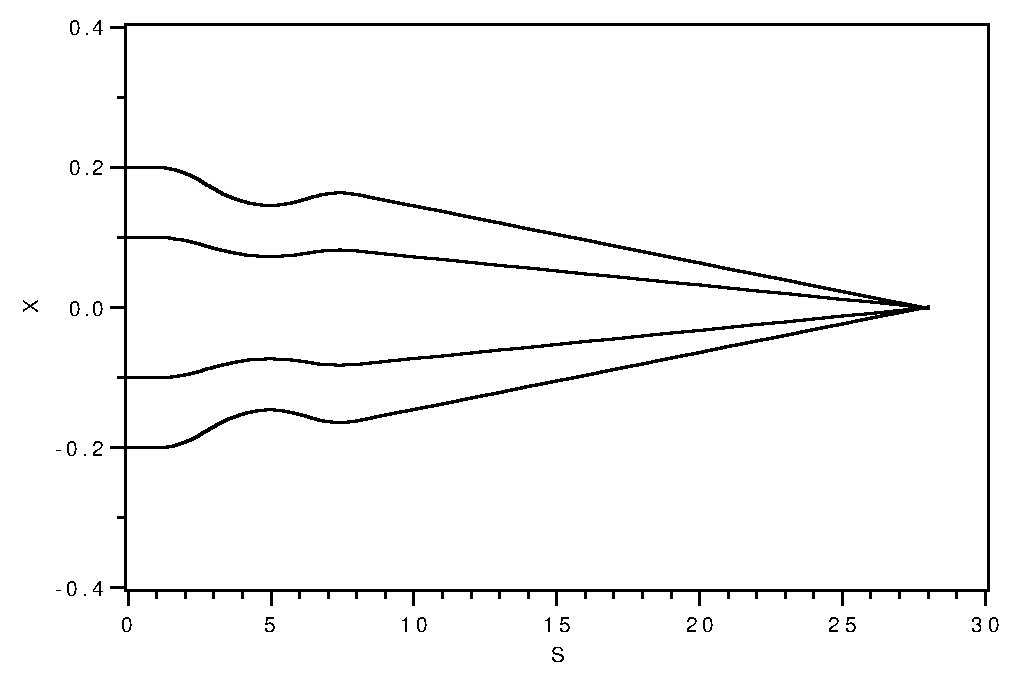
\includegraphics{fig10_17a}
  \caption{Spot-forming system ray plot for 4 initial rays launched in the
horizontal plane.}
\end{figure}

\newpage
\begin{figure}[htbp]
\renewcommand{\thefigure}{\thesection.\arabic{figure}}
  \centering
  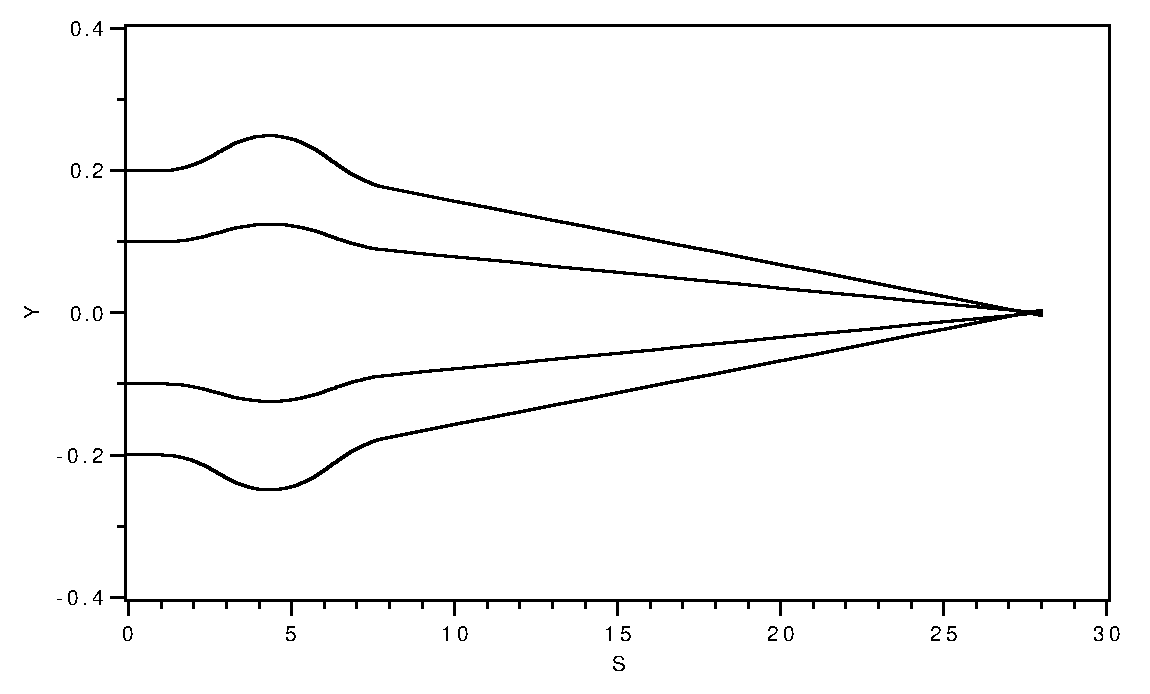
\includegraphics{fig10_17b}
  \caption{Spot-forming system ray plot for 4 initial rays launched in the
vertical plane.}
\end{figure}

\newpage
\begin{footnotesize}
\begin{verbatim}
Exhibit 10.10a
Contents of file 13 that specifies initial
conditions for 4 rays in the horizontal plane:

-.2 0 0 0 0 0
+.2 0 0 0 0 0
-.1 0 0 0 0 0
+.1 0 0 0 0 0


Exhibit 10.10b
Contents of file 20 that specifies instructions for the sq command
for writing out horizontal position coordinates for the 4 rays
whose initial conditions are specified in Exhibit 10.10a, and for
writing out path-length data:

 1  z(  1,1)
 2  z(  2,1)
 3  z(  3,1)
 4  z(  4,1)
 5        pl


Exhibit 10.10c
First few lines of file 30 that contains data written in response
to the wsq command.  In accord with the order presented in Exhibit
10.10b, the first 4 columns are the horizontal (X) position
coordinates of rays 1 through 4, respectively, and the last column
gives path-length data:

 -2.00000E-01  2.00000E-01 -1.00000E-01  1.00000E-01  0.00000E+00
 -2.00000E-01  2.00000E-01 -1.00000E-01  1.00000E-01  5.00000E-02
 -2.00000E-01  2.00000E-01 -1.00000E-01  1.00000E-01  1.00000E-01
 -2.00000E-01  2.00000E-01 -1.00000E-01  1.00000E-01  1.50000E-01
 -2.00000E-01  2.00000E-01 -1.00000E-01  1.00000E-01  2.00000E-01
 -2.00000E-01  2.00000E-01 -1.00000E-01  1.00000E-01  2.50000E-01
 -2.00000E-01  2.00000E-01 -1.00000E-01  1.00000E-01  3.00000E-01
 -2.00000E-01  2.00000E-01 -1.00000E-01  1.00000E-01  3.50000E-01
 -2.00000E-01  2.00000E-01 -1.00000E-01  1.00000E-01  4.00000E-01
 -2.00000E-01  2.00000E-01 -1.00000E-01  1.00000E-01  4.50000E-01
 -2.00000E-01  2.00000E-01 -1.00000E-01  1.00000E-01  5.00000E-01
 -2.00000E-01  2.00000E-01 -1.00000E-01  1.00000E-01  5.50000E-01
 -2.00000E-01  2.00000E-01 -1.00000E-01  1.00000E-01  6.00000E-01
 -2.00000E-01  2.00000E-01 -1.00000E-01  1.00000E-01  6.50000E-01
 -2.00000E-01  2.00000E-01 -1.00000E-01  1.00000E-01  7.00000E-01
 -2.00000E-01  2.00000E-01 -1.00000E-01  1.00000E-01  7.50000E-01
 -2.00000E-01  2.00000E-01 -1.00000E-01  1.00000E-01  8.00000E-01
 -2.00000E-01  2.00000E-01 -1.00000E-01  1.00000E-01  8.50000E-01
 -2.00000E-01  2.00000E-01 -1.00000E-01  1.00000E-01  9.00000E-01
 -2.00000E-01  2.00000E-01 -1.00000E-01  1.00000E-01  9.50000E-01
 -2.00000E-01  2.00000E-01 -1.00000E-01  1.00000E-01  1.00000E+00
 -2.00000E-01  2.00000E-01 -1.00000E-01  1.00000E-01  1.00000E+00
 -1.99868E-01  1.99868E-01 -9.99132E-02  9.99132E-02  1.15000E+00
 -1.99306E-01  1.99306E-01 -9.96320E-02  9.96320E-02  1.30000E+00
 -1.98369E-01  1.98369E-01 -9.91641E-02  9.91641E-02  1.45000E+00


Exhibit 10.10d
Contents of file 13 that specifies initial
conditions for 4 rays in the vertical plane:

0 0 -.2 0 0 0
0 0 +.2 0 0 0
0 0 +.1 0 0 0
0 0 -.1 0 0 0


Exhibit 10.10e
Contents of file 20 that specifies instructions for the sq command
for writing out vertical position coordinates for the 4 rays
whose initial conditions are specified in Exhibit 10.10d, and for
writing out path-length data:

 1  z(  1,3)
 2  z(  2,3)
 3  z(  3,3)
 4  z(  4,3)
 5        pl
 #

Exhibit 10.10f
***MARYLIE 3.0***
Prerelease Development Version 6/17/99
Copyright 1987 Alex J. Dragt
All rights reserved

Data input complete; going into #labor.
#comment
 Exhibit 10.10
      This is a MARYLIE run that demonstrates the production of ray plot data
 for the simple spot forming system of Section 2.2.  To do this all quads and
 drifts are split in 10 pieces, except for the final long drift which is split
 in 20 pieces.  The system is also slightly modified by preceding it with 2
 short drifts.   More precisely, since the elements are split in pieces,
 tracking is done piece by piece.

 The beam parameters are those for 50 MeV protons.

#beam
  1.03527440851950
 5.328901960570000E-002
  1.00000000000000
  1.00000000000000
#menu
 pli0     pli
  0.000000000000000E+00
 cdrs     drft
  0.500000000000000
 cdrl     drft
   20.0026000000000
 chfq     quad
   1.50000000000000      8.630000000000000E-02   1.00000000000000
   1.00000000000000
 chdq     quad
   3.00000000000000     -8.289450000000000E-02   1.00000000000000
   1.00000000000000
 drs/10   drft
  5.000000000000000E-02
 drl/20   drft
   1.00013000000000
 inhfq    quad
  0.000000000000000E+00  8.630000000000000E-02   1.00000000000000
  0.000000000000000E+00
 outhfq   quad
  0.000000000000000E+00  8.630000000000000E-02  0.000000000000000E+00
   1.00000000000000
 inhdq    quad
  0.000000000000000E+00 -8.289450000000000E-02   1.00000000000000
  0.000000000000000E+00
 outhdq   quad
  0.000000000000000E+00 -8.289450000000000E-02  0.000000000000000E+00
   1.00000000000000
 hfq/10   quad
  0.150000000000000      8.630000000000000E-02  0.000000000000000E+00
  0.000000000000000E+00
 hdq/10   quad
  0.300000000000000     -8.289450000000000E-02  0.000000000000000E+00
  0.000000000000000E+00
 fileout  pmif
   1.00000000000000       12.0000000000000       3.00000000000000
 mapout   ptm
   3.00000000000000       3.00000000000000      0.000000000000000E+00
  0.000000000000000E+00   1.00000000000000
 inv      inv
 wcl10    wcl
   3.00000000000000       10.0000000000000       3.00000000000000
 iden     iden
 raysin   rt
   13.0000000000000       14.0000000000000      -1.00000000000000
  0.000000000000000E+00  0.000000000000000E+00  0.000000000000000E+00
 rt       rt
  0.000000000000000E+00   14.0000000000000       5.00000000000000
   1.00000000000000       1.00000000000000      0.000000000000000E+00
 sq       sq
   20.0000000000000      0.000000000000000E+00   1.00000000000000
   1.00000000000000
 wsq      wsq
   1.00000000000000       1.00000000000000       30.0000000000000
   1.00000000000000       2.00000000000000      0.000000000000000E+00
 scmap    stm
   1.00000000000000
 stmap    stm
   2.00000000000000
 gcmap    gtm
   1.00000000000000       1.00000000000000
 gtmap    gtm
   2.00000000000000       2.00000000000000
 end      end
#lines
 hfq
     1*inhfq      10*hfq/10      1*outhfq
 hdq
     1*inhdq      10*hdq/10      1*outhdq
 drs
    10*drs/10
 drl
    20*drl/20
 trip
     1*hfq         1*drs         1*hdq         1*drs         1*hfq
 spot
     2*drs         1*trip        1*drl
 ctrip
     1*chfq        1*cdrs        1*chdq        1*cdrs        1*chfq
 cspot
     2*cdrs        1*ctrip       1*cdrl
 %spot
     1*%           1*drs/10      1*%           1*drs/10      1*%        &
     1*drs/10      1*%           1*drs/10      1*%           1*drs/10   &
     1*%           1*drs/10      1*%           1*drs/10      1*%        &
     1*drs/10      1*%           1*drs/10      1*%           1*drs/10   &
     1*%           1*drs/10      1*%           1*drs/10      1*%        &
     1*drs/10      1*%           1*drs/10      1*%           1*drs/10   &
     1*%           1*drs/10      1*%           1*drs/10      1*%        &
     1*drs/10      1*%           1*drs/10      1*%           1*drs/10   &
     1*%           1*inhfq       1*%           1*hfq/10      1*%        &
     1*hfq/10      1*%           1*hfq/10      1*%           1*hfq/10   &
     1*%           1*hfq/10      1*%           1*hfq/10      1*%        &
     1*hfq/10      1*%           1*hfq/10      1*%           1*hfq/10   &
     1*%           1*hfq/10      1*%           1*outhfq      1*%        &
     1*drs/10      1*%           1*drs/10      1*%           1*drs/10   &
     1*%           1*drs/10      1*%           1*drs/10      1*%        &
     1*drs/10      1*%           1*drs/10      1*%           1*drs/10   &
     1*%           1*drs/10      1*%           1*drs/10      1*%        &
     1*inhdq       1*%           1*hdq/10      1*%           1*hdq/10   &
     1*%           1*hdq/10      1*%           1*hdq/10      1*%        &
     1*hdq/10      1*%           1*hdq/10      1*%           1*hdq/10   &
     1*%           1*hdq/10      1*%           1*hdq/10      1*%        &
     1*hdq/10      1*%           1*outhdq      1*%           1*drs/10   &
     1*%           1*drs/10      1*%           1*drs/10      1*%        &
     1*drs/10      1*%           1*drs/10      1*%           1*drs/10   &
     1*%           1*drs/10      1*%           1*drs/10      1*%        &
     1*drs/10      1*%           1*drs/10      1*%           1*inhfq    &
     1*%           1*hfq/10      1*%           1*hfq/10      1*%        &
     1*hfq/10      1*%           1*hfq/10      1*%           1*hfq/10   &
     1*%           1*hfq/10      1*%           1*hfq/10      1*%        &
     1*hfq/10      1*%           1*hfq/10      1*%           1*hfq/10   &
     1*%           1*outhfq      1*%           1*drl/20      1*%        &
     1*drl/20      1*%           1*drl/20      1*%           1*drl/20   &
     1*%           1*drl/20      1*%           1*drl/20      1*%        &
     1*drl/20      1*%           1*drl/20      1*%           1*drl/20   &
     1*%           1*drl/20      1*%           1*drl/20      1*%        &
     1*drl/20      1*%           1*drl/20      1*%           1*drl/20   &
     1*%           1*drl/20      1*%           1*drl/20      1*%        &
     1*drl/20      1*%           1*drl/20      1*%           1*drl/20   &
     1*%           1*drl/20      1*%
 %
     1*work
 work
     1*rt          1*scmap       1*gtmap       1*gcmap       1*stmap    &
     1*pli0        1*wsq         1*iden
 setup
     1*raysin      1*iden        1*stmap       1*sq
#lumps
#loops
 lspot
     1*spot
#labor
    1*fileout
    1*setup
    1*%spot
    1*end

*******************************
* Response to raysin command: *
*******************************

    4 ray(s) read in from file  13

*******************************
* Response to the command sq: *
*******************************

 In subroutine sq
accept  1:    z(  1,1)
accept  2:    z(  2,1)
accept  3:    z(  3,1)
accept  4:    z(  4,1)
accept  5:          pl

 Aims/quantities selected :
No.     item      present value
----------------------------------
 1  z(  1,1) =     -0.200000000
 2  z(  2,1) =      0.200000000
 3  z(  3,1) =     -0.100000000
 4  z(  4,1) =      0.100000000
 5        pl =      0.000000000E+00

end of MARYLIE run
\end{verbatim}
\end{footnotesize}

\section{Production of Beam Moment Plots}\index{plots} \index{beam moment plots} \index{moment}
\label{prodbeam}
The production of beam moment plots is similar to the production of
lattice function and ray plots, and again requires 4 steps:

\begin{enumerate}
\item Specifying at what lattice locations beam moments or rms spreads
are to be calculated.
\item Calculating various geometric properties of the lattice, such as
path length, at these locations and arranging to have these
quantities written out onto a file.
\item Arranging to have the beam moments calculated at these same locations
and the desired results written out onto the same file.
\item Using the file generated in steps 2 and 3 above to produce beam
moment plots.
\end{enumerate}
The production of beam moment plot data is illustrated in this section
for the case of the spot-forming system of sections 2.2 and 10.10.  It
follows that steps 1 and 4 above are the same as those required to
produce ray plots for the spot-forming system.  (See section 10.10).\index{spot forming system}

Steps 2 and 3 require further explanation.  Examination of the {\em \#labor}
component of Exhibit 10.11c shows that it is identical to that in Exhibit
10.10f.  However, inspection of the {\em \#lines} component shows that
there is now the line {\em setup1} that has the contents

\begin{footnotesize}
\begin{verbatim}
setup1
     1*momgen      1*sq
\end{verbatim}
\end{footnotesize}
and that the line {\em momgen}, which contains the commands for
generating initial moments, has the contents

\begin{footnotesize}
\begin{verbatim}
momgen
     1*ps3         1*bgen        1*gbuf2       1*mapout      1*stm1     &
     1*iden        1*tws         1*mapout      1*snor        1*gbuf1    &
     1*mapout      1*amap        1*gbuf1       1*mapout      1*stm1     &
     1*iden
\end{verbatim}
\end{footnotesize}
The contents of {\em momgen} are somewhat analogous to those in the line
{\em makeic} in Exhibit 10.7a.  The commands {\em ps3} and {\em bgen} now
are used to generate moments which are fetched, exhibited at the terminal, and placed in
storage location 1 with the commands {\em gbuf2}, {\em mapout}, and {\em
stm1}.  See sections 8.14 and 8.34.  Subsequently a linear map with specified twiss
parameters is produced by {\em tws} and exhibited by {\em mapout}.  This
map is then analyzed by {\em snor} to produce a corresponding ${\cal A}$
that is fetched and exhibited by {\em gbuf1} and {\em mapout}.  See
section 8.8.  The map ${\cal A}$ is then applied by {\em amap} to the
moments produced earlier (and stored in location 1) to produce a set of
moments matched to {\em tws}.  See section 8.17.  The resulting moments are fetched by {\em
gbuf1}, exhibited by {\em mapout}, and put in storage location 1 by {\em stm1}
for subsequent use.  Finally, the current transfer map is reset to the
identity by the command {\em iden}.  Note that all the {\em mapout}
commands are used only to verify intermediate results, and need not be
invoked once one is confident all calculations are proceeding properly.

The other difference from the ray plot example is in the line {\em \%}:

\begin{footnotesize}
\begin{verbatim}
%
     1*work1
\end{verbatim}
\end{footnotesize}
It contains in turn the line {\em work1}
\begin{footnotesize}
\begin{verbatim}
work1
     1*pli0       1*samap       1*wsq
\end{verbatim}
\end{footnotesize}
This line invokes the command {\em pli0} to put path-length information
in the fitting/writing array.  It next invokes {\em samap} (a {\em silent} {\em amap} command) and the
expected {\em wsq} command required to write out results.  The {\em
samap} command applies the current total transfer map (which, unlike the
case of Exhibit 10.10f of the previous section, is now
being accumulated directly) to the initial moments that are in storage location 1
to obtain current transformed moments.  Again see section 8.17.

Exhibit 10.11a displays the instructions for {\em sq}.  Reference to the
description of {\em amap} in section 8.17 shows that the buffer 2 matrix
contents {\em bm2(1,1)}, {\em bm2(2,2)}, {\em bm2(3,3)}, and {\em
bm2(4,4)} are the root-mean-square spread quantities $\sqrt{\langle
X^2\rangle}$, $\sqrt{\langle P_x^2\rangle}$, $\sqrt{\langle Y^2\rangle}$,
and $\sqrt{\langle
P_y^2\rangle}$, respectively.  Also, the buffer 1 entry {\em bm1(1,2)} is
the moment $\langle XP_x\rangle$.  Thanks to the {\em wsq} command,
these quantities are written to file 30 along with path length along the
design orbit.  See Exhibit 10.11b.  Figures 11.1 through 11.5 show beam spread
and moment plots produced from file 30.  Finally, Exhibit 10.11c shows the
\Mary run itself.

\newpage
\begin{figure}[htbp]
\renewcommand{\thefigure}{\thesection.\arabic{figure}}
  \centering
  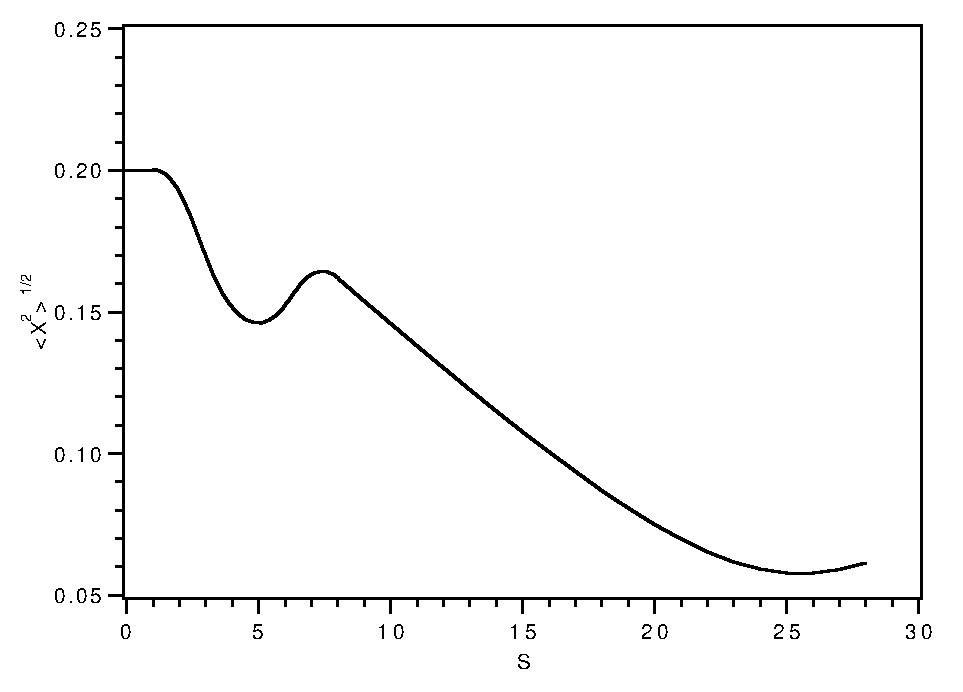
\includegraphics{fig10_18a}
  \caption{Spot-forming system plot of the rms horizontal position
spread $\sqrt{\langle X^2\rangle}$.}
\end{figure}

\newpage
\begin{figure}[htbp]
\renewcommand{\thefigure}{\thesection.\arabic{figure}}
  \centering
  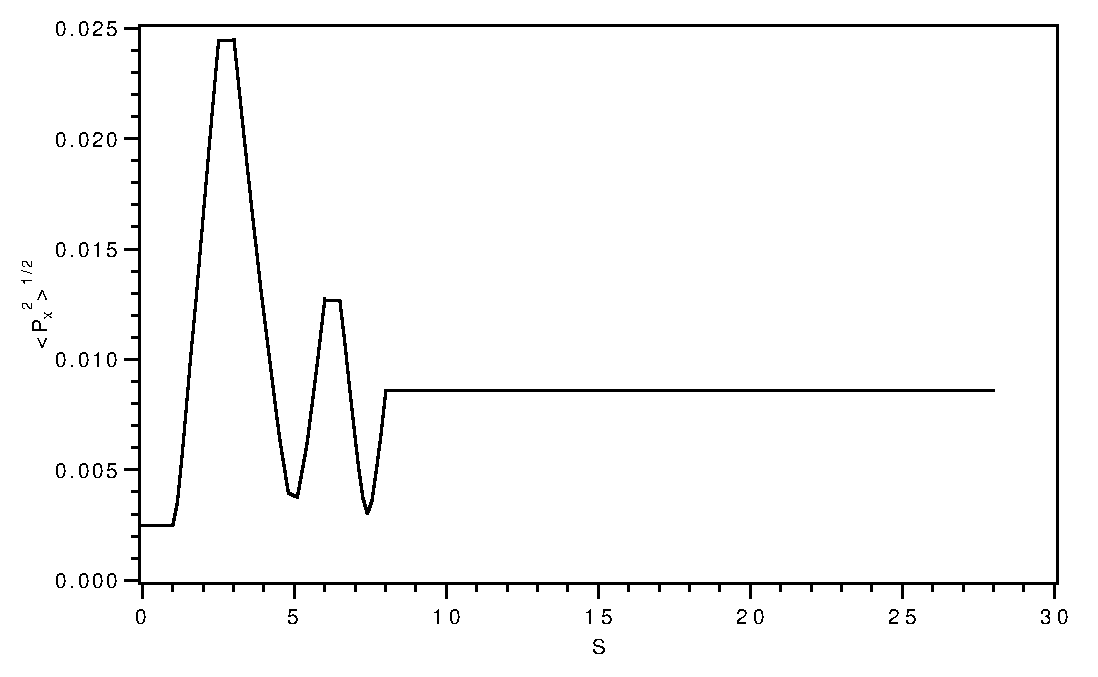
\includegraphics{fig10_18b}
  \caption{Spot-forming system plot of the rms horizontal momentum
spread $\sqrt{\langle P_x^2\rangle}$.}
\end{figure}

\newpage
\begin{figure}[htbp]
\renewcommand{\thefigure}{\thesection.\arabic{figure}}
  \centering
  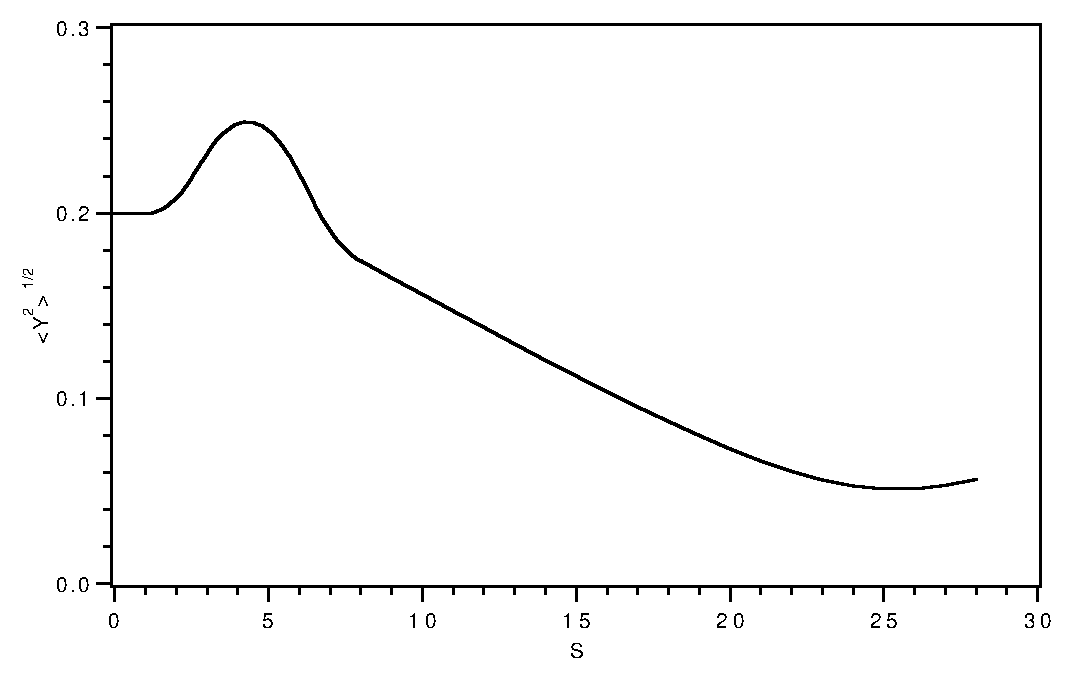
\includegraphics{fig10_18c}
  \caption{Spot-forming system plot of the rms vertical position
spread $\sqrt{\langle Y^2\rangle}$.}
\end{figure}

\newpage
\begin{figure}[htbp]
\renewcommand{\thefigure}{\thesection.\arabic{figure}}
  \centering
  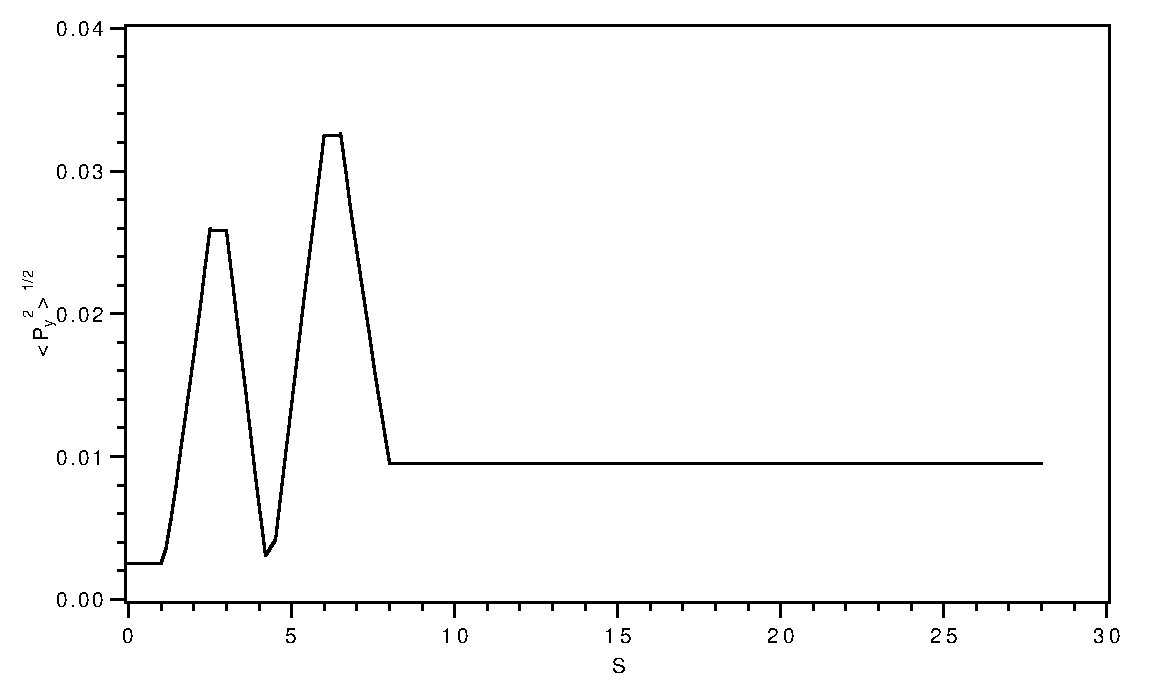
\includegraphics{fig10_18d}
  \caption{Spot-forming system plot of the rms vertical momentum
spread $\sqrt{\langle P_y^2\rangle}$.}
\end{figure}

\newpage
\begin{figure}[htbp]
\renewcommand{\thefigure}{\thesection.\arabic{figure}}
  \centering
  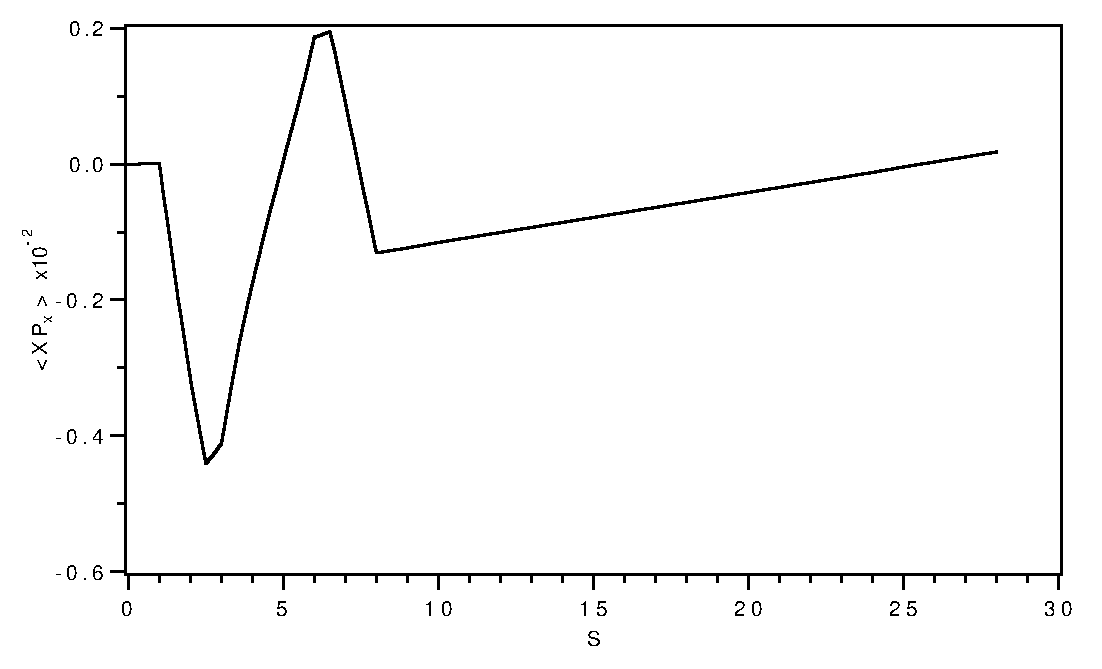
\includegraphics{fig10_18e}
  \caption{Spot-forming system plot of the horizontal moment
$\langle XP_x\rangle$.}
\end{figure}

\newpage
\begin{footnotesize}
\begin{verbatim}
Exhibit 10.11a
Contents of file 20 that specifies instructions for the sq command
for writing out the spread and moment quantities sqrt<XX>,
sqrt<PxPx>, sqrt<YY>, sqrt<PyPy>, <XPx>, and path length.

 1  bm2(1,1)
 2  bm2(2,2)
 3  bm2(3,3)
 4  bm2(4,4)
 5  bm1(1,2)
 6        pl


Exhibit 10.11b
First few lines of file 30 that contains data written in response to
the wsq command.  In accord with the ordering specified in Exhibit 10.11a
above, the first 4 columns are the spread and moment quantities sqrt<XX>,
sqrt<PxPx>, sqrt<YY>, sqrt<PyPy>, <XPx>, respectively, and the last column
is path length (pl).

  2.00000E-01  2.50000E-03  2.00000E-01  2.50000E-03  0.00000E+00  0.00000E+00
  2.00000E-01  2.50000E-03  2.00000E-01  2.50000E-03  3.12503E-07  5.00000E-02
  2.00000E-01  2.50000E-03  2.00000E-01  2.50000E-03  6.25006E-07  1.00000E-01
  2.00000E-01  2.50000E-03  2.00000E-01  2.50000E-03  9.37509E-07  1.50000E-01
  2.00001E-01  2.50000E-03  2.00001E-01  2.50000E-03  1.25001E-06  2.00000E-01

Exhibit 10.11c
***MARYLIE 3.0***
Prerelease Development Version 6/17/99
Copyright 1987 Alex J. Dragt
All rights reserved

Data input complete; going into #labor.
#comment
 Exhibit 10.11
 This is a MARYLIE run that demonstrates the production of beam moment
 plot data for the simple spot forming system of Section 2.2.  To do this all
 quads and drifts are split in 10 pieces, except for the final long drift
 which is split in 20 pieces.  The system is also slightly modified by
 preceding it with 2 short drifts.

 Transformed moments are computed from the initial moments using the
 accumulated transfer map.  See the contents of the line work1.

 Alternatively, transformed moments could be computed from the
 moments just preceding using just the map for the current element
 piece.  See the contents of the line work2 which could be used in place
 of work1.  (In this case one should also use setup2 in place of setup1.)
 This approach is the "moment" analog of element-by-element (actually
 piece-by-piece) tracking.

 The beam parameters are those for 50 MeV protons.

#beam
  1.03527440851950
 5.328901960570000E-002
  1.00000000000000
  1.00000000000000
#menu
 pli0     pli
  0.000000000000000E+00
 cdrs     drft
  0.500000000000000
 cdrl     drft
   20.0026000000000
 chfq     quad
   1.50000000000000      8.630000000000000E-02   1.00000000000000
   1.00000000000000
 chdq     quad
   3.00000000000000     -8.289450000000000E-02   1.00000000000000
   1.00000000000000
 drs/10   drft
  5.000000000000000E-02
 drl/20   drft
   1.00013000000000
 inhfq    quad
  0.000000000000000E+00  8.630000000000000E-02   1.00000000000000
  0.000000000000000E+00
 outhfq   quad
  0.000000000000000E+00  8.630000000000000E-02  0.000000000000000E+00
   1.00000000000000
 inhdq    quad
  0.000000000000000E+00 -8.289450000000000E-02   1.00000000000000
  0.000000000000000E+00
 outhdq   quad
  0.000000000000000E+00 -8.289450000000000E-02  0.000000000000000E+00
   1.00000000000000
 hfq/10   quad
  0.150000000000000      8.630000000000000E-02  0.000000000000000E+00
  0.000000000000000E+00
 hdq/10   quad
  0.300000000000000     -8.289450000000000E-02  0.000000000000000E+00
  0.000000000000000E+00
 fileout  pmif
   1.00000000000000       12.0000000000000       3.00000000000000
 mapout   ptm
   3.00000000000000       3.00000000000000      0.000000000000000E+00
  0.000000000000000E+00   1.00000000000000
 inv      inv
 wcl10    wcl
   3.00000000000000       10.0000000000000       3.00000000000000
 iden     iden
 raysin   rt
   13.0000000000000       14.0000000000000      -1.00000000000000
  0.000000000000000E+00  0.000000000000000E+00  0.000000000000000E+00
 rt       rt
  0.000000000000000E+00   14.0000000000000       5.00000000000000
   1.00000000000000       1.00000000000000      0.000000000000000E+00
 sq       sq
   20.0000000000000      0.000000000000000E+00   1.00000000000000
   1.00000000000000
 wsq      wsq
   1.00000000000000       1.00000000000000       30.0000000000000
   1.00000000000000       2.00000000000000      0.000000000000000E+00
 bgen     bgen
   2.00000000000000       2.00000000000000      0.000000000000000E+00
   123.000000000000       1.00000000000000       3.00000000000000
 ps3      ps3
  5.000000000000000E-04  5.000000000000000E-04  0.000000000000000E+00
  0.000000000000000E+00  0.000000000000000E+00  0.000000000000000E+00
 gbuf1    gbuf
   2.00000000000000       1.00000000000000
 gbuf2    gbuf
   2.00000000000000       2.00000000000000
 twx      twsm
   1.00000000000000       86.0000000000000      0.000000000000000E+00
   80.0000000000000
 twy      twsm
   2.00000000000000       96.0000000000000      0.000000000000000E+00
   80.0000000000000
 amap     amap
   2.00000000000000       1.00000000000000      -1.00000000000000
  0.000000000000000E+00  0.000000000000000E+00  0.000000000000000E+00
 samap    amap
   2.00000000000000      0.000000000000000E+00  -1.00000000000000
  0.000000000000000E+00  0.000000000000000E+00  0.000000000000000E+00
 stm1     stm
   1.00000000000000
 snor     snor
  0.000000000000000E+00  0.000000000000000E+00  0.000000000000000E+00
  0.000000000000000E+00  0.000000000000000E+00
 scmap    stm
   2.00000000000000
 stmap    stm
   3.00000000000000
 gcmap    gtm
   1.00000000000000       2.00000000000000
 gtmap    gtm
   2.00000000000000       3.00000000000000
 end      end
#lines
 hfq
     1*inhfq      10*hfq/10      1*outhfq
 hdq
     1*inhdq      10*hdq/10      1*outhdq
 drs
    10*drs/10
 drl
    20*drl/20
 trip
     1*hfq         1*drs         1*hdq         1*drs         1*hfq
 spot
     2*drs         1*trip        1*drl
 ctrip
     1*chfq        1*cdrs        1*chdq        1*cdrs        1*chfq
 cspot
     2*cdrs        1*ctrip       1*cdrl
 %spot
     1*%           1*drs/10      1*%           1*drs/10      1*%        &
     1*drs/10      1*%           1*drs/10      1*%           1*drs/10   &
     1*%           1*drs/10      1*%           1*drs/10      1*%        &
     1*drs/10      1*%           1*drs/10      1*%           1*drs/10   &
     1*%           1*drs/10      1*%           1*drs/10      1*%        &
     1*drs/10      1*%           1*drs/10      1*%           1*drs/10   &
     1*%           1*drs/10      1*%           1*drs/10      1*%        &
     1*drs/10      1*%           1*drs/10      1*%           1*drs/10   &
     1*%           1*inhfq       1*%           1*hfq/10      1*%        &
     1*hfq/10      1*%           1*hfq/10      1*%           1*hfq/10   &
     1*%           1*hfq/10      1*%           1*hfq/10      1*%        &
     1*hfq/10      1*%           1*hfq/10      1*%           1*hfq/10   &
     1*%           1*hfq/10      1*%           1*outhfq      1*%        &
     1*drs/10      1*%           1*drs/10      1*%           1*drs/10   &
     1*%           1*drs/10      1*%           1*drs/10      1*%        &
     1*drs/10      1*%           1*drs/10      1*%           1*drs/10   &
     1*%           1*drs/10      1*%           1*drs/10      1*%        &
     1*inhdq       1*%           1*hdq/10      1*%           1*hdq/10   &
     1*%           1*hdq/10      1*%           1*hdq/10      1*%        &
     1*hdq/10      1*%           1*hdq/10      1*%           1*hdq/10   &
     1*%           1*hdq/10      1*%           1*hdq/10      1*%        &
     1*hdq/10      1*%           1*outhdq      1*%           1*drs/10   &
     1*%           1*drs/10      1*%           1*drs/10      1*%        &
     1*drs/10      1*%           1*drs/10      1*%           1*drs/10   &
     1*%           1*drs/10      1*%           1*drs/10      1*%        &
     1*drs/10      1*%           1*drs/10      1*%           1*inhfq    &
     1*%           1*hfq/10      1*%           1*hfq/10      1*%        &
     1*hfq/10      1*%           1*hfq/10      1*%           1*hfq/10   &
     1*%           1*hfq/10      1*%           1*hfq/10      1*%        &
     1*hfq/10      1*%           1*hfq/10      1*%           1*hfq/10   &
     1*%           1*outhfq      1*%           1*drl/20      1*%        &
     1*drl/20      1*%           1*drl/20      1*%           1*drl/20   &
     1*%           1*drl/20      1*%           1*drl/20      1*%        &
     1*drl/20      1*%           1*drl/20      1*%           1*drl/20   &
     1*%           1*drl/20      1*%           1*drl/20      1*%        &
     1*drl/20      1*%           1*drl/20      1*%           1*drl/20   &
     1*%           1*drl/20      1*%           1*drl/20      1*%        &
     1*drl/20      1*%           1*drl/20      1*%           1*drl/20   &
     1*%           1*drl/20      1*%
 %
     1*work1
 work1
     1*pli0        1*samap       1*wsq
 work2
     1*scmap       1*samap       1*gbuf1       1*stm1        1*gtmap    &
     1*gcmap       1*stmap       1*pli0        1*wsq         1*iden
 setup1
     1*momgen      1*sq
 setup2
     1*momgen      1*iden        1*stmap       1*sq
 momgen
     1*ps3         1*bgen        1*gbuf2       1*mapout      1*stm1     &
     1*iden        1*tws         1*mapout      1*snor        1*gbuf1    &
     1*mapout      1*amap        1*gbuf1       1*mapout      1*stm1     &
     1*iden
 tws
     1*twx         1*twy
#lumps
#loops
 lspot
     1*spot
#labor
    1*fileout
    1*setup1
    1*%spot
    1*end

*********************************
* Response to the command bgen: *
*********************************

 analytically computed values of selected moments
 values of <x*x>, <x*px>, <px*px>:
 5.000000000000000E-004  0.000000000000000E+000  5.000000000000000E-004
 values of <y*y>, <y*py>, <py*py>:
 5.000000000000000E-004  0.000000000000000E+000  5.000000000000000E-004
 values of <t*t>, <t*pt>, <pt*pt>:
 0.000000000000000E+000  0.000000000000000E+000  0.000000000000000E+000

*********************************************
* Moments written in "map" form in response *
* to the gbuf2 and mapout commands:         *
*********************************************

matrix for map is :

 5.00000E-04  0.00000E+00  0.00000E+00  0.00000E+00  0.00000E+00  0.00000E+00
 0.00000E+00  5.00000E-04  0.00000E+00  0.00000E+00  0.00000E+00  0.00000E+00
 0.00000E+00  0.00000E+00  5.00000E-04  0.00000E+00  0.00000E+00  0.00000E+00
 0.00000E+00  0.00000E+00  0.00000E+00  5.00000E-04  0.00000E+00  0.00000E+00
 0.00000E+00  0.00000E+00  0.00000E+00  0.00000E+00  0.00000E+00  0.00000E+00
 0.00000E+00  0.00000E+00  0.00000E+00  0.00000E+00  0.00000E+00  0.00000E+00

nonzero elements in generating polynomial are :

 f(  7)=f( 20 00 00 )= 5.00000000000000E-04
 f( 13)=f( 02 00 00 )= 5.00000000000000E-04
 f( 18)=f( 00 20 00 )= 5.00000000000000E-04
 f( 22)=f( 00 02 00 )= 5.00000000000000E-04
 f( 84)=f( 40 00 00 )= 5.62500000000000E-07
 f( 90)=f( 22 00 00 )= 1.87500000000000E-07
 f( 95)=f( 20 20 00 )= 1.87500000000000E-07
 f( 99)=f( 20 02 00 )= 1.87500000000000E-07
 f(140)=f( 04 00 00 )= 5.62500000000000E-07
 f(145)=f( 02 20 00 )= 1.87500000000000E-07
 f(149)=f( 02 02 00 )= 1.87500000000000E-07
 f(175)=f( 00 40 00 )= 5.62500000000000E-07
 f(179)=f( 00 22 00 )= 1.87500000000000E-07
 f(195)=f( 00 04 00 )= 5.62500000000000E-07

*********************************
* Response to the stm1 command: *
*********************************

map stored in location   1

************************************
* Map produced by the tws command: *
************************************

matrix for map is :

 6.97565E-02  7.98051E+01  0.00000E+00  0.00000E+00  0.00000E+00  0.00000E+00
-1.24696E-02  6.97565E-02  0.00000E+00  0.00000E+00  0.00000E+00  0.00000E+00
 0.00000E+00  0.00000E+00 -1.04528E-01  7.95618E+01  0.00000E+00  0.00000E+00
 0.00000E+00  0.00000E+00 -1.24315E-02 -1.04528E-01  0.00000E+00  0.00000E+00
 0.00000E+00  0.00000E+00  0.00000E+00  0.00000E+00  1.00000E+00  0.00000E+00
 0.00000E+00  0.00000E+00  0.00000E+00  0.00000E+00  0.00000E+00  1.00000E+00

nonzero elements in generating polynomial are :

*********************************
* Response to the snor command: *
*********************************

det in fxpt is     0.4110E+01

***********************************************
* The matching map script A written in        *
* response to the gbuf1 and mapout commands:  *
***********************************************

matrix for map is :

 8.94427E+00  0.00000E+00  0.00000E+00  0.00000E+00  0.00000E+00  0.00000E+00
 0.00000E+00  1.11803E-01  0.00000E+00  0.00000E+00  0.00000E+00  0.00000E+00
 0.00000E+00  0.00000E+00  8.94427E+00  0.00000E+00  0.00000E+00  0.00000E+00
 0.00000E+00  0.00000E+00  0.00000E+00  1.11803E-01  0.00000E+00  0.00000E+00
 0.00000E+00  0.00000E+00  0.00000E+00  0.00000E+00  1.00000E+00  0.00000E+00
 0.00000E+00  0.00000E+00  0.00000E+00  0.00000E+00  0.00000E+00  1.00000E+00

nonzero elements in generating polynomial are :

*********************************
* Response to the amap command: *
*********************************

map gotten from location   1

******************************************
* Moments written in "map" form by amap: *
******************************************

 transformed moments

matrix for map is :

 4.00000E-02  0.00000E+00  0.00000E+00  0.00000E+00  0.00000E+00  0.00000E+00
 0.00000E+00  6.25000E-06  0.00000E+00  0.00000E+00  0.00000E+00  0.00000E+00
 0.00000E+00  0.00000E+00  4.00000E-02  0.00000E+00  0.00000E+00  0.00000E+00
 0.00000E+00  0.00000E+00  0.00000E+00  6.25000E-06  0.00000E+00  0.00000E+00
 0.00000E+00  0.00000E+00  0.00000E+00  0.00000E+00  0.00000E+00  0.00000E+00
 0.00000E+00  0.00000E+00  0.00000E+00  0.00000E+00  0.00000E+00  0.00000E+00

nonzero elements in generating polynomial are :

 f(  7)=f( 20 00 00 )= 4.00000000000000E-02
 f( 13)=f( 02 00 00 )= 6.25000000000000E-06
 f( 18)=f( 00 20 00 )= 4.00000000000000E-02
 f( 22)=f( 00 02 00 )= 6.25000000000000E-06
 f( 84)=f( 40 00 00 )= 3.60000000000000E-03
 f( 90)=f( 22 00 00 )= 1.87500000000000E-07
 f( 95)=f( 20 20 00 )= 1.20000000000000E-03
 f( 99)=f( 20 02 00 )= 1.87500000000000E-07
 f(140)=f( 04 00 00 )= 8.78906250000000E-11
 f(145)=f( 02 20 00 )= 1.87500000000000E-07
 f(149)=f( 02 02 00 )= 2.92968750000000E-11
 f(175)=f( 00 40 00 )= 3.60000000000000E-03
 f(179)=f( 00 22 00 )= 1.87500000000000E-07
 f(195)=f( 00 04 00 )= 8.78906250000000E-11

***************************************************
* Response to the gbuf1 and mapout commands       *
* showing the contents of buffer 1 in "map" form: *
***************************************************

matrix for map is :

 4.00000E-02  0.00000E+00  0.00000E+00  0.00000E+00  0.00000E+00  0.00000E+00
 0.00000E+00  6.25000E-06  0.00000E+00  0.00000E+00  0.00000E+00  0.00000E+00
 0.00000E+00  0.00000E+00  4.00000E-02  0.00000E+00  0.00000E+00  0.00000E+00
 0.00000E+00  0.00000E+00  0.00000E+00  6.25000E-06  0.00000E+00  0.00000E+00
 0.00000E+00  0.00000E+00  0.00000E+00  0.00000E+00  0.00000E+00  0.00000E+00
 0.00000E+00  0.00000E+00  0.00000E+00  0.00000E+00  0.00000E+00  0.00000E+00

nonzero elements in generating polynomial are :

 f(  7)=f( 20 00 00 )= 4.00000000000000E-02
 f( 13)=f( 02 00 00 )= 6.25000000000000E-06
 f( 18)=f( 00 20 00 )= 4.00000000000000E-02
 f( 22)=f( 00 02 00 )= 6.25000000000000E-06
 f( 84)=f( 40 00 00 )= 3.60000000000000E-03
 f( 90)=f( 22 00 00 )= 1.87500000000000E-07
 f( 95)=f( 20 20 00 )= 1.20000000000000E-03
 f( 99)=f( 20 02 00 )= 1.87500000000000E-07
 f(140)=f( 04 00 00 )= 8.78906250000000E-11
 f(145)=f( 02 20 00 )= 1.87500000000000E-07
 f(149)=f( 02 02 00 )= 2.92968750000000E-11
 f(175)=f( 00 40 00 )= 3.60000000000000E-03
 f(179)=f( 00 22 00 )= 1.87500000000000E-07
 f(195)=f( 00 04 00 )= 8.78906250000000E-11

*********************************
* Response to the stm1 command: *
*********************************

map stored in location   1

*******************************
* Response to the sq command: *
*******************************

 In subroutine sq
accept  1:    bm2(1,1)
accept  2:    bm2(2,2)
accept  3:    bm2(3,3)
accept  4:    bm2(4,4)
accept  5:    bm1(1,2)
accept  6:          pl

 Aims/quantities selected :
No.     item      present value
----------------------------------
 1  bm2(1,1) =      0.200000000
 2  bm2(2,2) =      2.500000000E-03
 3  bm2(3,3) =      0.200000000
 4  bm2(4,4) =      2.500000000E-03
 5  bm1(1,2) =      0.000000000E+00
 6        pl =      0.000000000E+00

end of MARYLIE run
\end{verbatim}
\end{footnotesize}

\section{Production of Composite Plots with Geometry}\index{plots} \index{composite plots} \index{geometry}
\label{compplots}
Sections 10.9, 10.10, and 10.11 illustrated the production of simple plots
of various quantities as a function of path length.  The path-length data
for these plots were obtained using {\em pli} commands.  It is often useful to have various kinds of plots be accompanied by some
schematic, similar to those of figure 2.5.2, that illustrates the
underlying lattice.  Such plots are easily produced, from output files
written by the {\em geom} command, with the aid of the program POSTER.
See sections 1.4.2 and 8.38.  The {\em geom} command acts on {\em loops}
to provide detailed geometric information as well as path-length data.
The subsections below illustrate the use of the {\em geom} command.  As
will be seen, the use of {\em geom} rather than {\em pli} to provide
path-length information can also sometimes simplify the logic of some entries in the
Master Input File.\index{POSTER}

\subsection{Lattice Function Plots with Geometry}\index{lattice function plots}
\label{latfunplots}
Figures 10.12.1.1 and 10.12.1.2 show lattice function plots, with
additional geometrical data, for the Proton Storage Ring.  Exhibit
10.12.1f shows the \Mary run used to produce these plots.  Much of this
Master Input File is similar to that of Exhibit 10.9c.  However, there
are a few differences that are described below.

First, the line {\em setup} now takes the form
\begin{footnotesize}
\begin{verbatim}
setup
     1*iden       1*ring       1*stotmap       1*sq       1*iden
\end{verbatim}
\end{footnotesize}
There is now no need for a {\em pli0} command since, as will be seen,
path-length data will be provided by {\em geom}.  Correspondingly, there
is now no need to select {\em pl} in response to the {\em sq} command.
Exhibit 10.12.1a shows how file 20 is modified in this case.

Second, the line {\em \%} now takes the form
\begin{footnotesize}
\begin{verbatim}
%
     1*work       1*dp
\end{verbatim}
\end{footnotesize}
The line {\em work} specifies the work to be done, and is the same as
before in Exhibit 10.9c.  The entry {\em dp} is used in a subsequent
computation of geometrical properties of the lattice.  See section 6.26.

Third, the {\em \#labor} component of the Master Input File now has the
contents
\begin{footnotesize}
\begin{verbatim}
#labor
	 1*fileout
	 1*setup
	 1*%ring
	 1*l%ring
	 1*cgeom
	 1*merf
	 1*fin
\end{verbatim}
\end{footnotesize}

\newpage
\renewcommand{\thefigure}{\thesubsection.\arabic{figure}}
\begin{figure}[h]
  \centering
  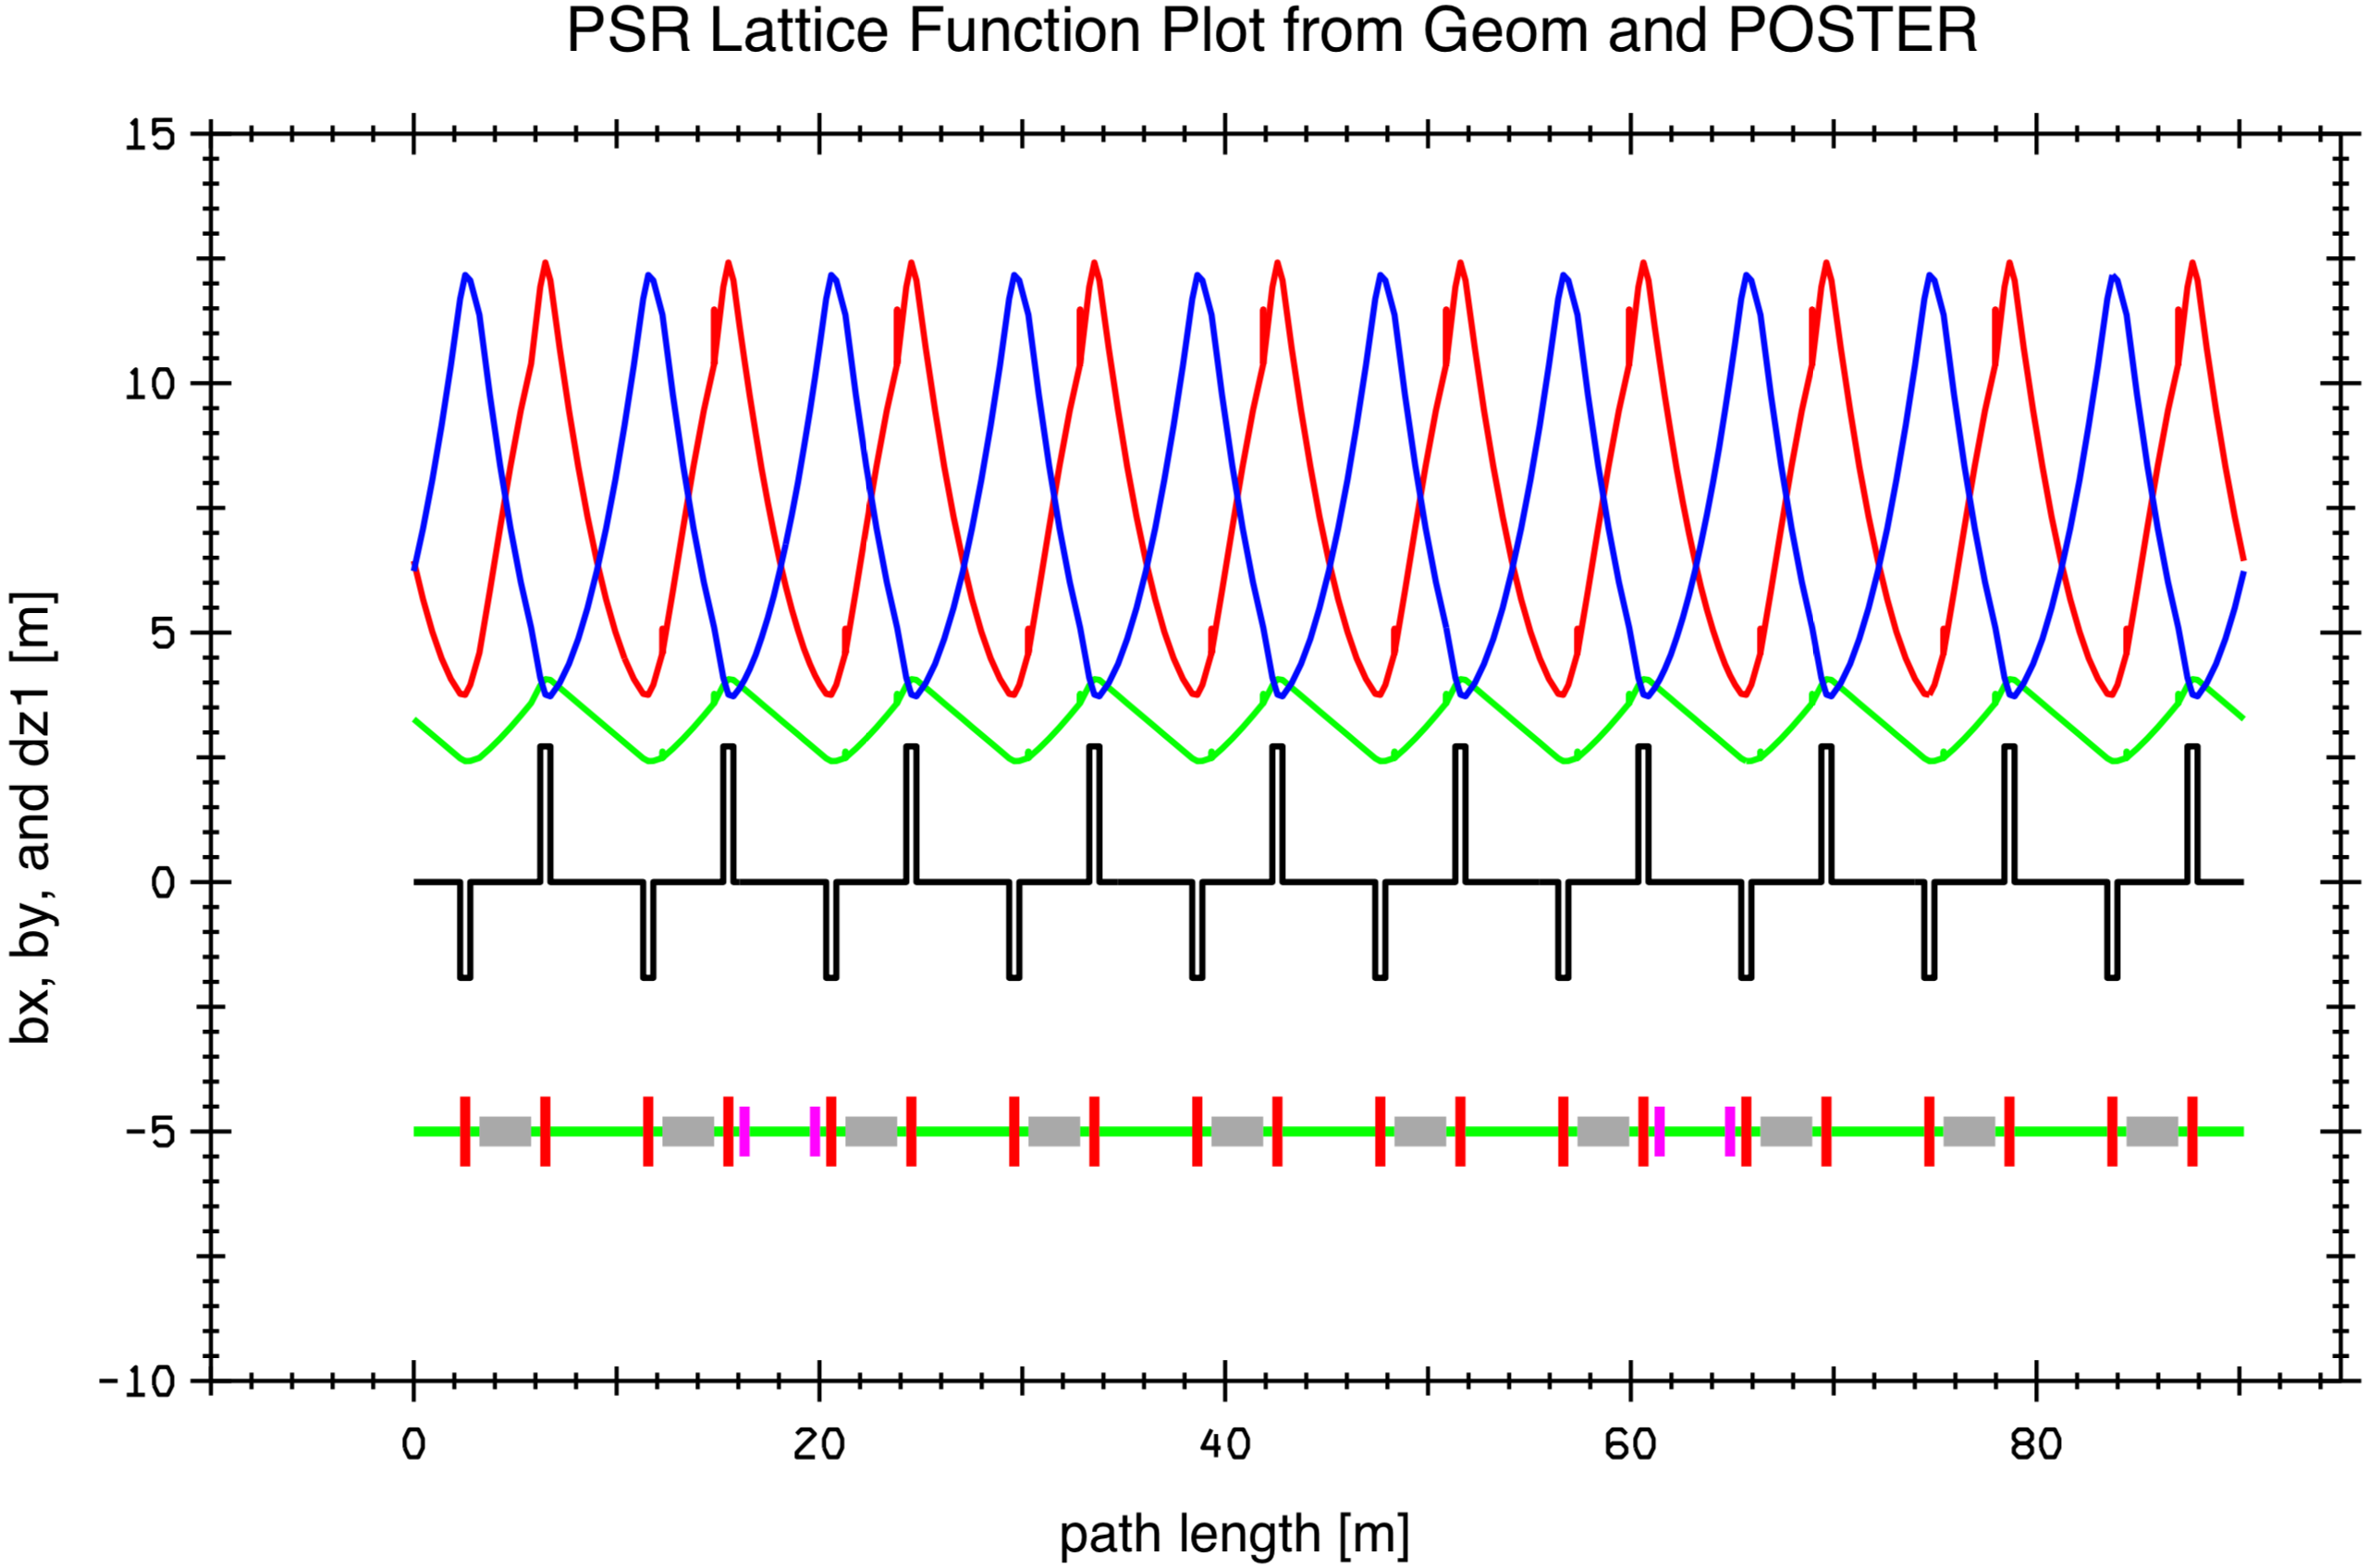
\includegraphics[scale=0.400]{lat}
  \caption{Various lattice functions for the Proton Storage Ring treated
in section 10.9 accompanied by a schematic of the lattice.  The
quadrupole gradient is also illustrated.}
\end{figure}

\newpage
\begin{figure}[h]
  \centering
  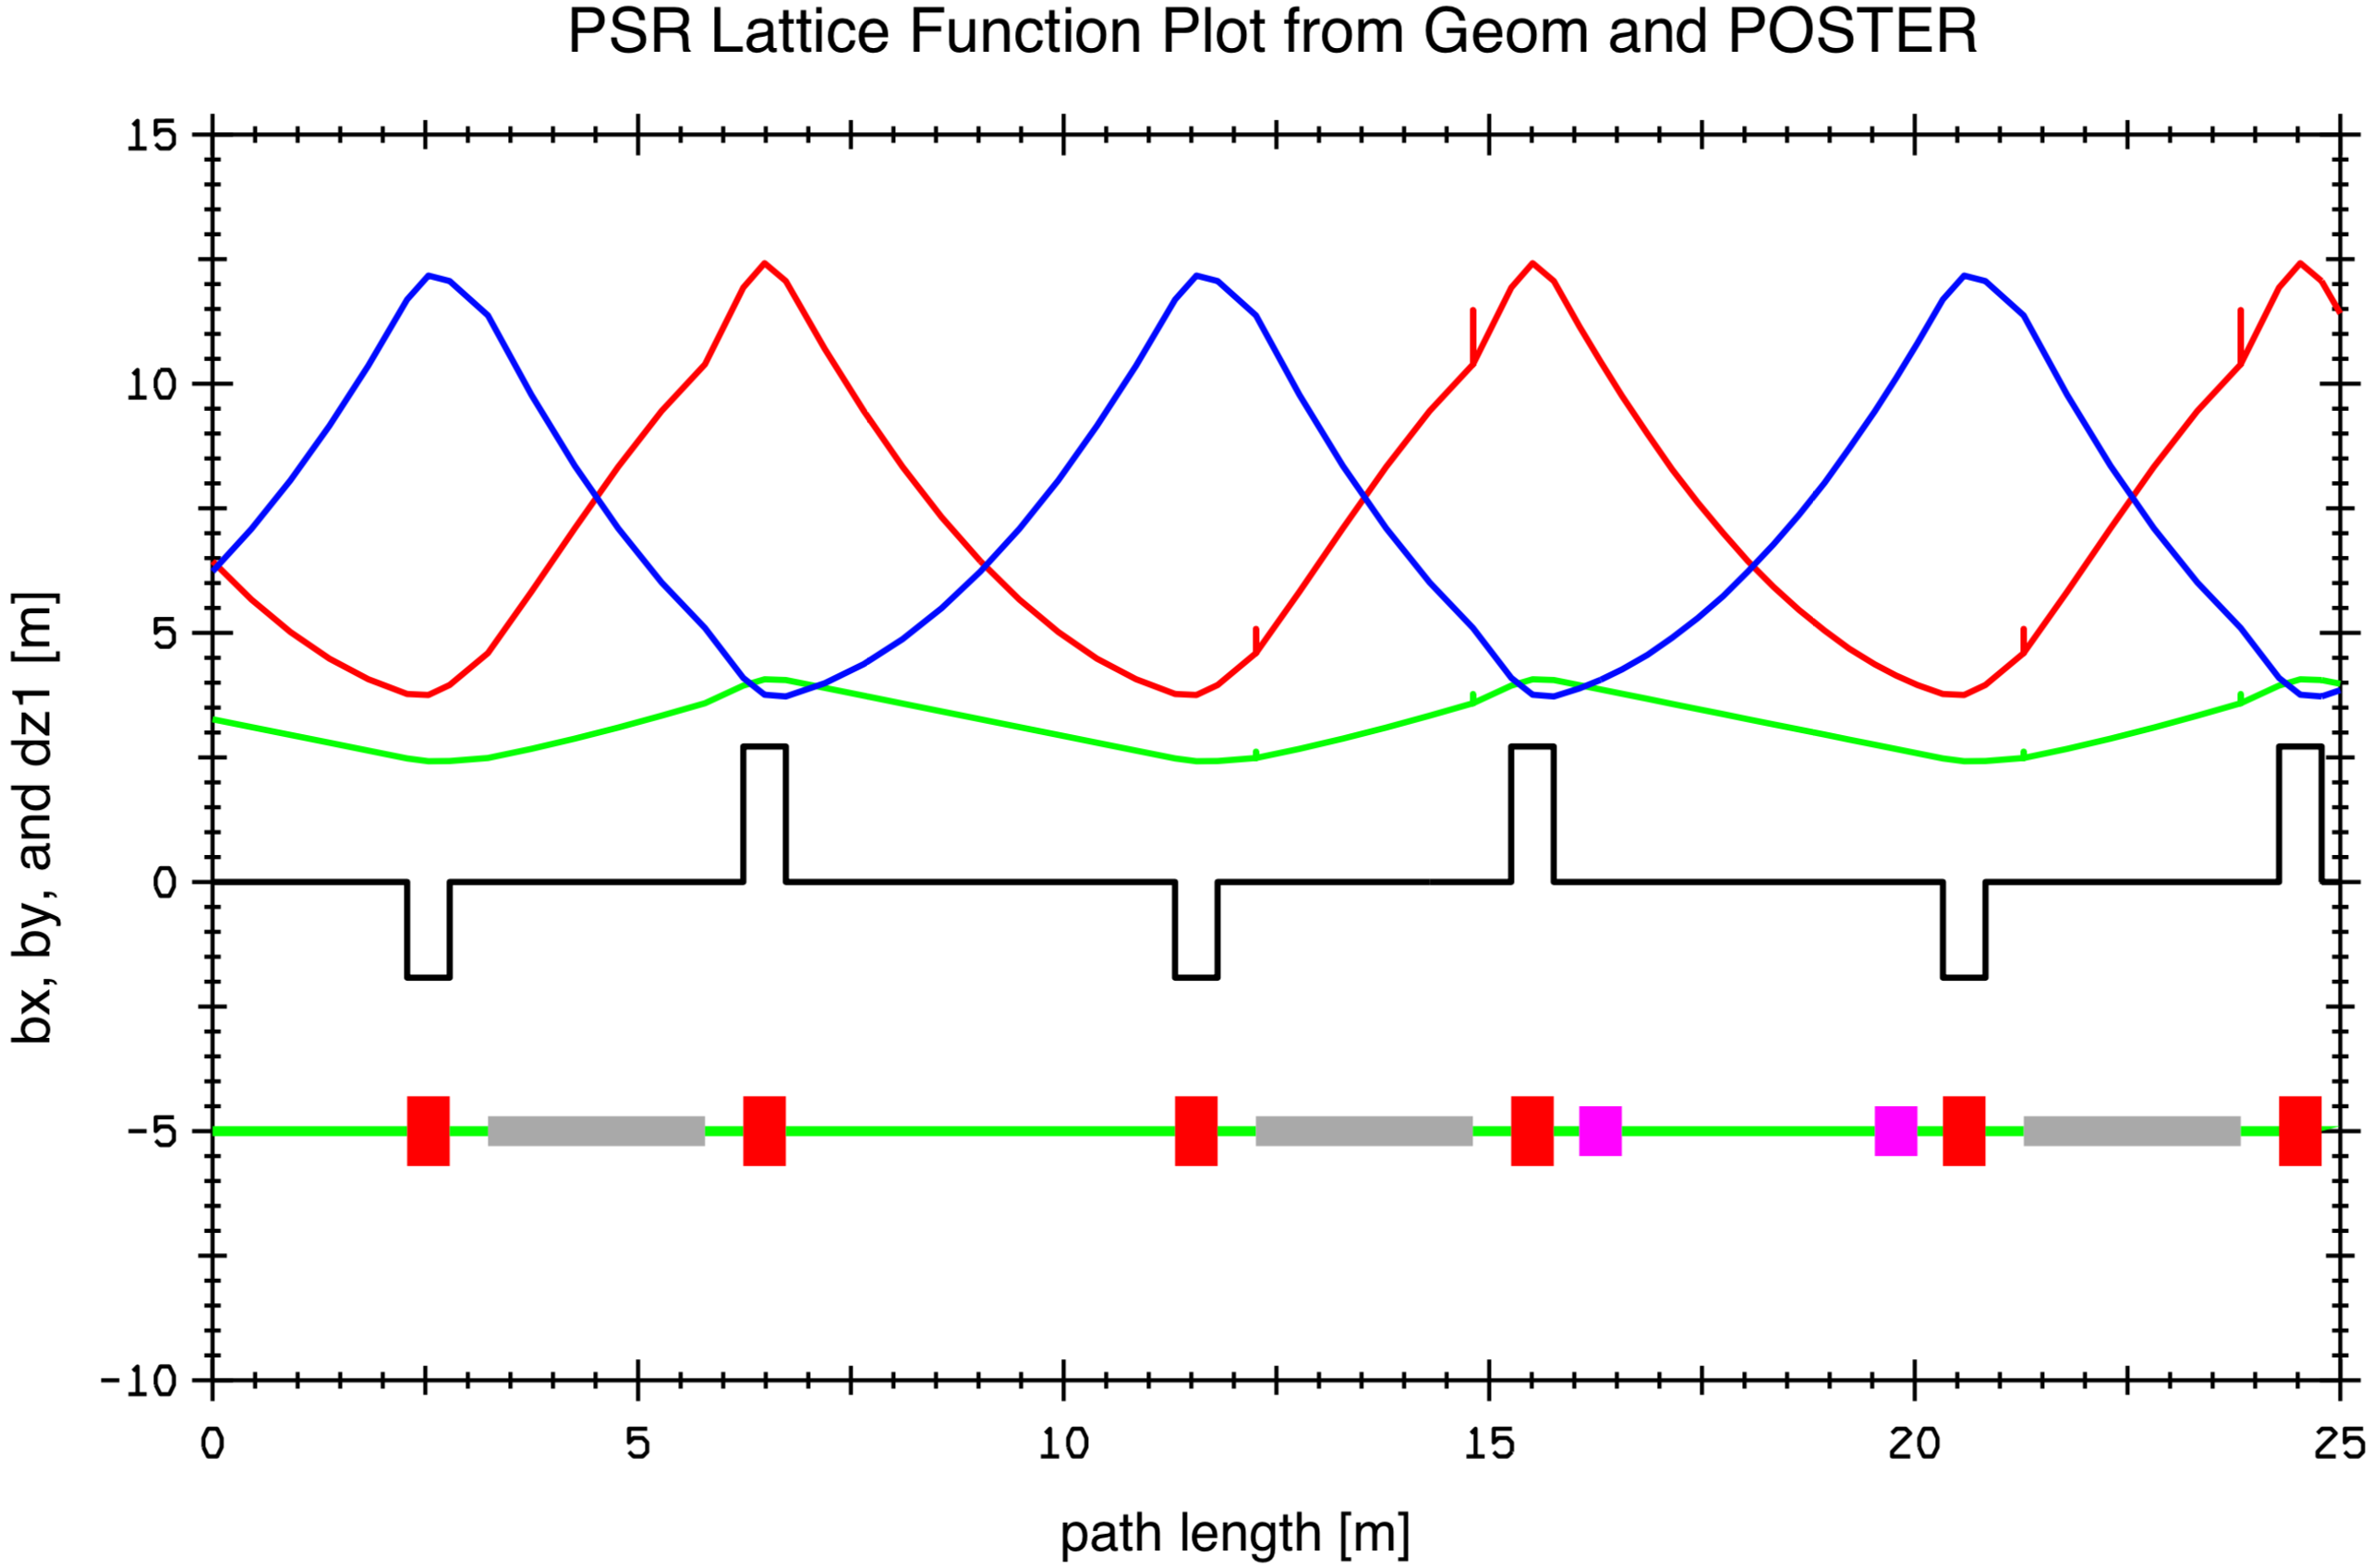
\includegraphics[scale=0.400]{latzoom}
  \caption{An expanded version of a portion of figure 10.12.1.1.}
\end{figure}

\newpage
\noindent The first 3 entries ({\em 1*fileout}, {\em 1*setup}, {\em 1*\%ring}) function as
before except that only lattice function, and not path-length, information
is written on file 30.  See Exhibit 10.12.1b.  The entry {\em 1*l\%ring}
invokes a {\em loop} whose contents is {\em \%ring}.  See the {\em
\#loops} component of Exhibit 10.12.1f.  The entry {\em cgeom} invokes a
line that contains a {\em geom} command preceded by the commands {\em ps1}
and {\em ps2} that set the parameters required by {\em geom}:

\begin{footnotesize}
\begin{verbatim}
cgeom
     1*ps1       1*ps2       1*geom
\end{verbatim}
\end{footnotesize}

So doing causes various geometric properties of the lattice to be
computed and written
to the external file IFILE, in this case file 40, at each occurrence of
the command {\em dp} (which in turn occurs in the line {\em \%}).  See
section 8.38.  Exhibit 10.12.1c shows the first few lines of file 40.  In
particular, the first column of file 40 is path length along the design
orbit.  Finally, the {\em merf} command in {\em \#labor} merges the first
column of file 40 with the remaining columns of file 30 and writes the
results on file 50.  (See the contents of {\em \#labor} and section
8.40.)  Exhibit 10.12.1d shows the
first few lines of file 50.  Note that the contents of Exhibits 10.12.1d
and 10.9b are identical except for the interchange of various columns.
Therefore, if desired, this file could be used to produce (with the aid
of any of a variety of graphics programs) simple lattice-function plots of the
form shown in section 10.9.

In addition to file 40 (which contains path-length and coordinate data),
{\em geom} also writes simple element description and path-length
information to file KFILE, in this case file 60.  See section 8.38.
Exhibit 10.12.1e shows the first few lines of file 60.  By processing with POSTER
simultaneously file 50 (written by {\em merf}) and file 60, it is
possible to produce plots accompanied by a schematic of the underlying
lattice.  Figures 12.1.1 and 12.1.2 show composite lattice plots produced in
this way for the Proton Storage Ring.

As mentioned in section 10.9, in the lattice function plots of figures
10.9.1 through 10.9.3 and 10.9.5 through
10.9.7 there are some unexpected spikes.  Inspection shows that these spikes
are also present in figures 12.1.1 and 12.1.2, and from these figures it is
clear that these spikes are associated with the entries and exits of
dipoles.  These spikes are unphysical, and are an artifact of the
procedure used to slice (split) the dipoles.

As described in sections 6.6 and 10.9, the slicing of parallel faced bends
entails use of the maps {\em inprot} and {\em ingbdy} at the entrance to
the dipole, and the use of the maps {\em outgbdy} and {\em outprot} at
the exit of the dipole.  It is these maps, which have no length and
therefore give results at the same path-length {\em s} value, that produce the
spikes.

Closer inspection of figures 12.1.1 and 12.1.2 shows that there are no spikes
associated with the first dipole, but there are spikes associated with
the subsequent dipoles.  There are no spikes associated with the first
dipole because, for the \Mary run that produced this figure, the
computation and writing out of lattice functions at points between {\em
inprot} and {\em ingbdy} and between {\em outgbdy} and {\em outprot}
were suppressed for the first dipole.  Comparison of the lines {\em
\%ring} in Exhibits 10.9c and 10.12.1f shows one (easily
reversible) way of doing this.  What has
been done is to replace by {\em \$} signs the {\em \%} signs that occur in the
first dipole between {\em inprot} and {\em ingbdy} and between {\em
outgbdy} and {\em outprot}.  The {\em \$} sign refers to the line

\begin{footnotesize}
\begin{verbatim}
$
     1*mark
\end{verbatim}
\end{footnotesize}

So doing replaces {\em work} and {\em dp} (which cause
computation and writing of lattice functions and geometric information) by the no effect marker
element {\em mark}.  See section 6.25.  Alternatively, one could simply
remove these {\em \%} signs.

\begin{footnotesize}
\begin{verbatim}
Exhibit 10.12.1a
Instructions in file 20 for the sq command:

 1  bf1( 28)
 2       dz1
 3       dz2
 4        bx
 5        by
 #

Exhibit 10.12.1b
First few lines of file 30 written as a result of the wsq command.
In agreement with Exhibit 10.12.1a above, the columns are bf1(28),
dz1, dz2, bx, and by, respectively:

 2.97958E-03  3.26669E+00 -3.44101E-01  6.43759E+00  6.23191E+00
 2.97958E-03  3.10933E+00 -3.44101E-01  5.66815E+00  7.08761E+00
 2.97958E-03  2.95198E+00 -3.44101E-01  5.01700E+00  8.06134E+00
 2.97958E-03  2.79462E+00 -3.44101E-01  4.48413E+00  9.15310E+00
 2.97958E-03  2.63727E+00 -3.44101E-01  4.06956E+00  1.03629E+01
 2.97958E-03  2.47991E+00 -3.44101E-01  3.77328E+00  1.16907E+01
-1.05970E-02  2.42416E+00 -1.02875E-01  3.75309E+00  1.21683E+01
-2.54879E-02  2.42827E+00  1.35811E-01  3.95404E+00  1.20626E+01

Exhibit 10.12.1c
First few lines of file 40 written as a result of the geom command.
The first column is path length along the design orbit:

 0.00000E+00  1.40000E+01  0.00000E+00  0.00000E+00  0.00000E+00  0.00000E+00
 4.57292E-01  1.40000E+01  0.00000E+00  4.57292E-01  1.81329E-09  0.00000E+00
 9.14584E-01  1.40000E+01  0.00000E+00  9.14584E-01  3.62659E-09  0.00000E+00
 1.37188E+00  1.40000E+01  0.00000E+00  1.37188E+00  5.43988E-09  0.00000E+00
 1.82917E+00  1.40000E+01  0.00000E+00  1.82917E+00  7.25318E-09  0.00000E+00
 2.28646E+00  1.40000E+01  0.00000E+00  2.28646E+00  9.06647E-09  0.00000E+00
 2.53646E+00  1.40000E+01  0.00000E+00  2.53646E+00  1.00578E-08  0.00000E+00
 2.78646E+00  1.40000E+01  0.00000E+00  2.78646E+00  1.10491E-08  0.00000E+00


Exhibit 10.12.1d
First few lines of file 50 written as a result of the merf command.
Note that the first column (path length) is the same as that in
Exhibit 10.12.1c above, and the remaining columns (lattice functions) are
the same as in Exhibit 10.12.1b:

  0.0000E+00  0.2980E-02  0.3267E+01 -0.3441E+00  0.6438E+01  0.6232E+01
  0.4573E+00  0.2980E-02  0.3109E+01 -0.3441E+00  0.5668E+01  0.7088E+01
  0.9146E+00  0.2980E-02  0.2952E+01 -0.3441E+00  0.5017E+01  0.8061E+01
  0.1372E+01  0.2980E-02  0.2795E+01 -0.3441E+00  0.4484E+01  0.9153E+01
  0.1829E+01  0.2980E-02  0.2637E+01 -0.3441E+00  0.4070E+01  0.1036E+02
  0.2286E+01  0.2980E-02  0.2480E+01 -0.3441E+00  0.3773E+01  0.1169E+02
  0.2536E+01 -0.1060E-01  0.2424E+01 -0.1029E+00  0.3753E+01  0.1217E+02
  0.2786E+01 -0.2549E-01  0.2428E+01  0.1358E+00  0.3954E+01  0.1206E+02

Exhibit 10.12.1e
First few lines of file 60 written as a result of the geom command.
This file provides simple element and path-length information:

drl/5     1  1  0.00000E+00  0.00000E+00  0.00000E+00  0.00000E+00
drl/5     1  1  4.57292E-01  0.00000E+00  0.00000E+00  0.00000E+00
drl/5     1  1  4.57292E-01  0.00000E+00  0.00000E+00  0.00000E+00
drl/5     1  1  9.14584E-01  0.00000E+00  0.00000E+00  0.00000E+00
drl/5     1  1  9.14584E-01  0.00000E+00  0.00000E+00  0.00000E+00
drl/5     1  1  1.37188E+00  0.00000E+00  0.00000E+00  0.00000E+00
drl/5     1  1  1.37188E+00  0.00000E+00  0.00000E+00  0.00000E+00
drl/5     1  1  1.82917E+00  0.00000E+00  0.00000E+00  0.00000E+00
drl/5     1  1  1.82917E+00  0.00000E+00  0.00000E+00  0.00000E+00
drl/5     1  1  2.28646E+00  0.00000E+00  0.00000E+00  0.00000E+00
inhdq     1  9  2.28646E+00  0.00000E+00  0.00000E+00 -1.92000E+00
inhdq     1  9  2.53646E+00  0.00000E+00  0.00000E+00 -1.92000E+00
outhdq    1  9  2.53646E+00  0.00000E+00  0.00000E+00 -1.92000E+00
outhdq    1  9  2.78646E+00  0.00000E+00  0.00000E+00 -1.92000E+00
drs       1  1  2.78646E+00  0.00000E+00  0.00000E+00  0.00000E+00


Exhibit 10.12.1f
***MARYLIE 3.0***
Prerelease Development Version 6/17/99
Copyright 1987 Alex J. Dragt
All rights reserved

Data input complete; going into #labor.
#comment

 Exhibit 10.12.1

 This is a MaryLie run that employs the geom and other type codes to
 produce lattice function and geometrical data using the PSR as an
 example.  The dipoles and the long and medium-long drifts are split into
 5 pieces.  Quads and sextupoles are split in two.  This run generates
 data for the entire ring.

 For the first dipole at the beginning of the line %ring, the computation
 and writing of lattice function and geometrical data (produced by the
 commands work and dp) is suppressed between inprot and ingbdy at the
 entrance to the dipole, and between outgbdy and outprot at the exit of
 the dipole.  This is accomplished by replacing % by $.  Here % is the
 name of the line

 %
     1*work        1*dp

 and $ is the name of the line

 $
     1*mark

 So doing removes from the lattice function plots (for the first dipole)
 the unphysical spikes that are an artifact of the slicing (splitting)
 procedure for dipoles.

#beam
  4.86914813175970
 0.849425847892200
  1.00000000000000
  1.00000000000000
#menu
 mark     mark
 drvs     drft
  0.300000000000000
 drs      drft
  0.450000000000000
 cdrml    drft
   1.48646000000000
 drml/5   drft
  0.297292000000000
 cdrl     drft
   2.28646000000000
 drl/5    drft
  0.457292000000000
 cbend    pbnd
   36.0000000000000      0.000000000000000E+00  0.500000000000000
   1.20000000000000
 inprot   prot
   18.0000000000000       1.00000000000000
 outprot  prot
   18.0000000000000       2.00000000000000
 infrng   frng
   18.0000000000000      0.000000000000000E+00  0.000000000000000E+00
   1.20000000000000       1.00000000000000
 outfrng  frng
   18.0000000000000      0.000000000000000E+00  0.000000000000000E+00
   1.20000000000000       2.00000000000000
 ingbdy   gbdy
  0.000000000000000E+00   18.0000000000000      0.000000000000000E+00
   1.20000000000000
 outgbdy  gbdy
  0.000000000000000E+00  0.000000000000000E+00   18.0000000000000
   1.20000000000000
 sbend/5  nbnd
   7.20000000000000      0.000000000000000E+00  0.500000000000000
   1.20000000000000      0.000000000000000E+00  0.000000000000000E+00
 chfq     quad
  0.500000000000000       2.72000000000000       1.00000000000000
   1.00000000000000
 inhfq    quad
  0.250000000000000       2.72000000000000       1.00000000000000
  0.000000000000000E+00
 outhfq   quad
  0.250000000000000       2.72000000000000      0.000000000000000E+00
   1.00000000000000
 chdq     quad
  0.500000000000000      -1.92000000000000       1.00000000000000
   1.00000000000000
 inhdq    quad
  0.250000000000000      -1.92000000000000       1.00000000000000
  0.000000000000000E+00
 outhdq   quad
  0.250000000000000      -1.92000000000000      0.000000000000000E+00
   1.00000000000000
 chcs     sext
  0.500000000000000      0.000000000000000E+00
 hcs/2    sext
  0.250000000000000      0.000000000000000E+00
 cvcs     sext
  0.500000000000000      0.000000000000000E+00
 vcs/2    sext
  0.250000000000000      0.000000000000000E+00
 fileout  pmif
   1.00000000000000       12.0000000000000       3.00000000000000
 tasm     tasm
   2.00000000000000      1.000000000000000E-03   12.0000000000000
  0.000000000000000E+00   10.0000000000000      0.000000000000000E+00
 stasm    tasm
   2.00000000000000      1.000000000000000E-03   2.00000000000000
  0.000000000000000E+00  0.000000000000000E+00  0.000000000000000E+00
 snor     snor
  0.000000000000000E+00  0.000000000000000E+00  0.000000000000000E+00
  0.000000000000000E+00  0.000000000000000E+00
 iden     iden
 inv      inv
 dp       dp
 stotmap  stm
   1.00000000000000
 gtotmap  gtm
   1.00000000000000       1.00000000000000
 scurmap  stm
   2.00000000000000
 gcurmap  gtm
   1.00000000000000       2.00000000000000
 sq       sq
   20.0000000000000      0.000000000000000E+00   1.00000000000000
   1.00000000000000
 wsq      wsq
   1.00000000000000       1.00000000000000       30.0000000000000
   1.00000000000000       2.00000000000000      0.000000000000000E+00
 wcl10    wcl
   3.00000000000000       10.0000000000000       3.00000000000000
 wcl15    wcl
   3.00000000000000       15.0000000000000       3.00000000000000
 geom     geom
   3.00000000000000      0.000000000000000E+00  0.000000000000000E+00
   1.00000000000000       2.00000000000000      0.000000000000000E+00
 ps1      ps1
   14.0000000000000      0.000000000000000E+00  0.000000000000000E+00
  0.000000000000000E+00  0.000000000000000E+00  0.000000000000000E+00
 ps2      ps2
   40.0000000000000      0.000000000000000E+00   60.0000000000000
   70.0000000000000      0.000000000000000E+00   1.00000000000000
 merf     usr12
   40.0000000000000       30.0000000000000       50.0000000000000
   1.00000000000000       5.00000000000000      0.000000000000000E+00
 setzero  zer
  0.000000000000000E+00  1.000000000000000E-10  0.000000000000000E+00
 mapout   ptm
   3.00000000000000       3.00000000000000      0.000000000000000E+00
  0.000000000000000E+00   1.00000000000000
 fin      end
#lines
 drml
     5*drml/5
 drl
     5*drl/5
 bend
     1*inprot      1*infrng      1*ingbdy      5*sbend/5     1*outgbdy  &
     1*outfrng     1*outprot
 hfq
     1*inhfq       1*outhfq
 hdq
     1*inhdq       1*outhdq
 hcs
     2*hcs/2
 vcs
     2*vcs/2
 nsex
     1*drl         1*hdq         1*drs         1*bend        1*drs      &
     1*hfq         1*drl
 tsex
     1*drl         1*hdq         1*drs         1*bend        1*drs      &
     1*hfq         1*drvs        1*hcs         1*drml
 lsex
     1*drml        1*vcs         1*drvs        1*hdq         1*drs      &
     1*bend        1*drs         1*hfq         1*drl
 half
     1*nsex        1*tsex        1*lsex        1*nsex        1*nsex
 ring
     2*half
 %tsex
     1*%           1*drl/5       1*%           1*drl/5       1*%        &
     1*drl/5       1*%           1*drl/5       1*%           1*drl/5    &
     1*%           1*inhdq       1*%           1*outhdq      1*%        &
     1*drs         1*%           1*inprot      1*%           1*infrng   &
     1*%           1*ingbdy      1*%           1*sbend/5     1*%        &
     1*sbend/5     1*%           1*sbend/5     1*%           1*sbend/5  &
     1*%           1*sbend/5     1*%           1*outgbdy     1*%        &
     1*outfrng     1*%           1*outprot     1*%           1*drs      &
     1*%           1*inhfq       1*%           1*outhfq      1*%        &
     1*drvs        1*%           1*hcs/2       1*%           1*hcs/2    &
     1*%           1*drml/5      1*%           1*drml/5      1*%        &
     1*drml/5      1*%           1*drml/5      1*%           1*drml/5   &
     1*%
 %ring
     1*%           1*drl/5       1*%           1*drl/5       1*%        &
     1*drl/5       1*%           1*drl/5       1*%           1*drl/5    &
     1*%           1*inhdq       1*%           1*outhdq      1*%        &
     1*drs         1*%           1*inprot      1*$           1*infrng   &
     1*$           1*ingbdy      1*%           1*sbend/5     1*%        &
     1*sbend/5     1*%           1*sbend/5     1*%           1*sbend/5  &
     1*%           1*sbend/5     1*%           1*outgbdy     1*$        &
     1*outfrng     1*$           1*outprot     1*%           1*drs      &
     1*%           1*inhfq       1*%           1*outhfq      1*%        &
     1*drl/5       1*%           1*drl/5       1*%           1*drl/5    &
     1*%           1*drl/5       1*%           1*drl/5       1*%        &
     1*drl/5       1*%           1*drl/5       1*%           1*drl/5    &
     1*%           1*drl/5       1*%           1*drl/5       1*%        &
     1*inhdq       1*%           1*outhdq      1*%           1*drs      &
     1*%           1*inprot      1*%           1*infrng      1*%        &
     1*ingbdy      1*%           1*sbend/5     1*%           1*sbend/5  &
     1*%           1*sbend/5     1*%           1*sbend/5     1*%        &
     1*sbend/5     1*%           1*outgbdy     1*%           1*outfrng  &
     1*%           1*outprot     1*%           1*drs         1*%        &
     1*inhfq       1*%           1*outhfq      1*%           1*drvs     &
     1*%           1*hcs/2       1*%           1*hcs/2       1*%        &
     1*drml/5      1*%           1*drml/5      1*%           1*drml/5   &
     1*%           1*drml/5      1*%           1*drml/5      1*%        &
     1*drml/5      1*%           1*drml/5      1*%           1*drml/5   &
     1*%           1*drml/5      1*%           1*drml/5      1*%        &
     1*vcs/2       1*%           1*vcs/2       1*%           1*drvs     &
     1*%           1*inhdq       1*%           1*outhdq      1*%        &
     1*drs         1*%           1*inprot      1*%           1*infrng   &
     1*%           1*ingbdy      1*%           1*sbend/5     1*%        &
     1*sbend/5     1*%           1*sbend/5     1*%           1*sbend/5  &
     1*%           1*sbend/5     1*%           1*outgbdy     1*%        &
     1*outfrng     1*%           1*outprot     1*%           1*drs      &
     1*%           1*inhfq       1*%           1*outhfq      1*%        &
     1*drl/5       1*%           1*drl/5       1*%           1*drl/5    &
     1*%           1*drl/5       1*%           1*drl/5       1*%        &
     1*drl/5       1*%           1*drl/5       1*%           1*drl/5    &
     1*%           1*drl/5       1*%           1*drl/5       1*%        &
     1*inhdq       1*%           1*outhdq      1*%           1*drs      &
     1*%           1*inprot      1*%           1*infrng      1*%        &
     1*ingbdy      1*%           1*sbend/5     1*%           1*sbend/5  &
     1*%           1*sbend/5     1*%           1*sbend/5     1*%        &
     1*sbend/5     1*%           1*outgbdy     1*%           1*outfrng  &
     1*%           1*outprot     1*%           1*drs         1*%        &
     1*inhfq       1*%           1*outhfq      1*%           1*drl/5    &
     1*%           1*drl/5       1*%           1*drl/5       1*%        &
     1*drl/5       1*%           1*drl/5       1*%           1*drl/5    &
     1*%           1*drl/5       1*%           1*drl/5       1*%        &
     1*drl/5       1*%           1*drl/5       1*%           1*inhdq    &
     1*%           1*outhdq      1*%           1*drs         1*%        &
     1*inprot      1*%           1*infrng      1*%           1*ingbdy   &
     1*%           1*sbend/5     1*%           1*sbend/5     1*%        &
     1*sbend/5     1*%           1*sbend/5     1*%           1*sbend/5  &
     1*%           1*outgbdy     1*%           1*outfrng     1*%        &
     1*outprot     1*%           1*drs         1*%           1*inhfq    &
     1*%           1*outhfq      1*%           1*drl/5       1*%        &
     1*drl/5       1*%           1*drl/5       1*%           1*drl/5    &
     1*%           1*drl/5       1*%           1*drl/5       1*%        &
     1*drl/5       1*%           1*drl/5       1*%           1*drl/5    &
     1*%           1*drl/5       1*%           1*inhdq       1*%        &
     1*outhdq      1*%           1*drs         1*%           1*inprot   &
     1*%           1*infrng      1*%           1*ingbdy      1*%        &
     1*sbend/5     1*%           1*sbend/5     1*%           1*sbend/5  &
     1*%           1*sbend/5     1*%           1*sbend/5     1*%        &
     1*outgbdy     1*%           1*outfrng     1*%           1*outprot  &
     1*%           1*drs         1*%           1*inhfq       1*%        &
     1*outhfq      1*%           1*drl/5       1*%           1*drl/5    &
     1*%           1*drl/5       1*%           1*drl/5       1*%        &
     1*drl/5       1*%           1*drl/5       1*%           1*drl/5    &
     1*%           1*drl/5       1*%           1*drl/5       1*%        &
     1*drl/5       1*%           1*inhdq       1*%           1*outhdq   &
     1*%           1*drs         1*%           1*inprot      1*%        &
     1*infrng      1*%           1*ingbdy      1*%           1*sbend/5  &
     1*%           1*sbend/5     1*%           1*sbend/5     1*%        &
     1*sbend/5     1*%           1*sbend/5     1*%           1*outgbdy  &
     1*%           1*outfrng     1*%           1*outprot     1*%        &
     1*drs         1*%           1*inhfq       1*%           1*outhfq   &
     1*%           1*drvs        1*%           1*hcs/2       1*%        &
     1*hcs/2       1*%           1*drml/5      1*%           1*drml/5   &
     1*%           1*drml/5      1*%           1*drml/5      1*%        &
     1*drml/5      1*%           1*drml/5      1*%           1*drml/5   &
     1*%           1*drml/5      1*%           1*drml/5      1*%        &
     1*drml/5      1*%           1*vcs/2       1*%           1*vcs/2    &
     1*%           1*drvs        1*%           1*inhdq       1*%        &
     1*outhdq      1*%           1*drs         1*%           1*inprot   &
     1*%           1*infrng      1*%           1*ingbdy      1*%        &
     1*sbend/5     1*%           1*sbend/5     1*%           1*sbend/5  &
     1*%           1*sbend/5     1*%           1*sbend/5     1*%        &
     1*outgbdy     1*%           1*outfrng     1*%           1*outprot  &
     1*%           1*drs         1*%           1*inhfq       1*%        &
     1*outhfq      1*%           1*drl/5       1*%           1*drl/5    &
     1*%           1*drl/5       1*%           1*drl/5       1*%        &
     1*drl/5       1*%           1*drl/5       1*%           1*drl/5    &
     1*%           1*drl/5       1*%           1*drl/5       1*%        &
     1*drl/5       1*%           1*inhdq       1*%           1*outhdq   &
     1*%           1*drs         1*%           1*inprot      1*%        &
     1*infrng      1*%           1*ingbdy      1*%           1*sbend/5  &
     1*%           1*sbend/5     1*%           1*sbend/5     1*%        &
     1*sbend/5     1*%           1*sbend/5     1*%           1*outgbdy  &
     1*%           1*outfrng     1*%           1*outprot     1*%        &
     1*drs         1*%           1*inhfq       1*%           1*outhfq   &
     1*%           1*drl/5       1*%           1*drl/5       1*%        &
     1*drl/5       1*%           1*drl/5       1*%           1*drl/5    &
     1*%           1*drl/5       1*%           1*drl/5       1*%        &
     1*drl/5       1*%           1*drl/5       1*%           1*drl/5    &
     1*%           1*inhdq       1*%           1*outhdq      1*%        &
     1*drs         1*%           1*inprot      1*%           1*infrng   &
     1*%           1*ingbdy      1*%           1*sbend/5     1*%        &
     1*sbend/5     1*%           1*sbend/5     1*%           1*sbend/5  &
     1*%           1*sbend/5     1*%           1*outgbdy     1*%        &
     1*outfrng     1*%           1*outprot     1*%           1*drs      &
     1*%           1*inhfq       1*%           1*outhfq      1*%        &
     1*drl/5       1*%           1*drl/5       1*%           1*drl/5    &
     1*%           1*drl/5       1*%           1*drl/5       1*%
 %phalf
     1*nsex        1*%tsex       1*lsex        1*nsex        1*nsex
 %pring
     1*half        1*%phalf
 setup
     1*iden        1*ring        1*stotmap     1*sq          1*iden
 %
     1*work        1*dp
 work
     1*cpssmap     1*anal        1*wsq         1*restore
 cpssmap
     1*scurmap     1*inv         1*gtotmap     1*gcurmap
 restore
     1*iden        1*gcurmap
 anal
     1*stasm       1*snor
 $
     1*mark
 cgeom
     1*ps1         1*ps2         1*geom
#lumps
#loops
 ltsex
     1*tsex
 lring
     1*ring
 l%ring
     1*%ring
 l%pring
     1*%pring
#labor
    1*fileout
    1*setup
    1*%ring
    1*l%ring
    1*cgeom
    1*merf
    1*fin

*******************************
* Response to the sq command: *
*******************************

 In subroutine sq
accept  1:    bf1( 28)
accept  2:         dz1
accept  3:         dz2
accept  4:          bx
accept  5:          by

 Aims/quantities selected :
No.     item      present value
----------------------------------
 1  bf1( 28) =      0.000000000E+00
 2       dz1 =      0.000000000E+00
 3       dz2 =      0.000000000E+00
 4        bx =      0.000000000E+00
 5        by =      0.000000000E+00

*********************************
* Response to the merf command: *
*********************************

 number of lines read =         279

end of MARYLIE run
\end{verbatim}
\end{footnotesize}

\newpage
\subsection{Ray Plots with Geometry}\index{plots} \index{geometry} \index{ray plots with geometry}
\label{rayplots}
Figure 10.12.2.1 shows a ray plot, with additional geometric data, for the
spot-forming system of sections 2.2 and 10.10.  Exhibit 10.12.2f shows
the \Mary run used to produce this plot.  Much of this Master Input File
is similar to that of Exhibit 10.10f.  However, there are a few
differences that are described below.\index{spot forming system}

First, there is no need to store the total map since path-length data
will now be produced by a {\em geom} command.  Therefore the line {\em
setup} can take the simpler form
\begin{footnotesize}
\begin{verbatim}
setup
     1*raysin     1*sq
\end{verbatim}
\end{footnotesize}
Correspondingly, there is now no need to select {\em pl} in response to
the {\em sq} command.  Exhibit 10.12.2a shows
how file 20 is modified in this case.

Second, the line {\em \%} now takes the form
\begin{footnotesize}
\begin{verbatim}
%
     1*work      1*dp
\end{verbatim}
\end{footnotesize}
and the line {\em work}, which specifies the work to be done, can now take the
simple form
\begin{footnotesize}
\begin{verbatim}
work
     1*rt     1*wsq     1*iden
\end{verbatim}
\end{footnotesize}
When the line {\em work} is invoked at each occurrence of the $\%$ symbol
in the line {\em \%spot} (see Exhibit 10.12.2f) a ray trace will be
performed using the current map, selected results from this ray trace
will be written to an external file (in this case file 30) by the command
{\em wsq}, and the current map will be reset to the identity map as a
result of the command {\em iden}.  The entry {\em dp} in {\em \%}, which follows {\em
work}, is used in connection with {\em geom} in a subsequent computation of geometrical properties of
the spot-forming system.  See section 6.26.

Third, the {\em \#labor} component of the Master Input File now has the
contents
\begin{footnotesize}
\begin{verbatim}
#labor
	 1*fileout
	 1*setup
	 1*%spot
	 1*l%spot
	 1*cgeom
	 1*merf
	 1*end
\end{verbatim}
\end{footnotesize}

The first 3 entries ({\em 1*fileout}, {\em 1*setup}, {\em 1*\%spot})
function as before except that only ray, and not path-length, information
is written on file 30.  See Exhibit 10.12.2b.  The entry {\em 1*l\%spot}
invokes a {\em loop} whose contents is {\em \%spot}.  See the {\em \#loops}
component of Exhibit 10.12.2f.  The entry {\em cgeom} invokes a line that
contains a {\em geom} command preceded by the commands {\em ps1}
and {\em ps2} that set the parameters required by geom:
\begin{footnotesize}
\begin{verbatim}
cgeom
     1*ps1   1*ps2  1*geom
\end{verbatim}
\end{footnotesize}

\newpage
\renewcommand{\thefigure}{\thesubsection.\arabic{figure}}
\setcounter{figure}{0}
\begin{figure}[htp]
  \centering
  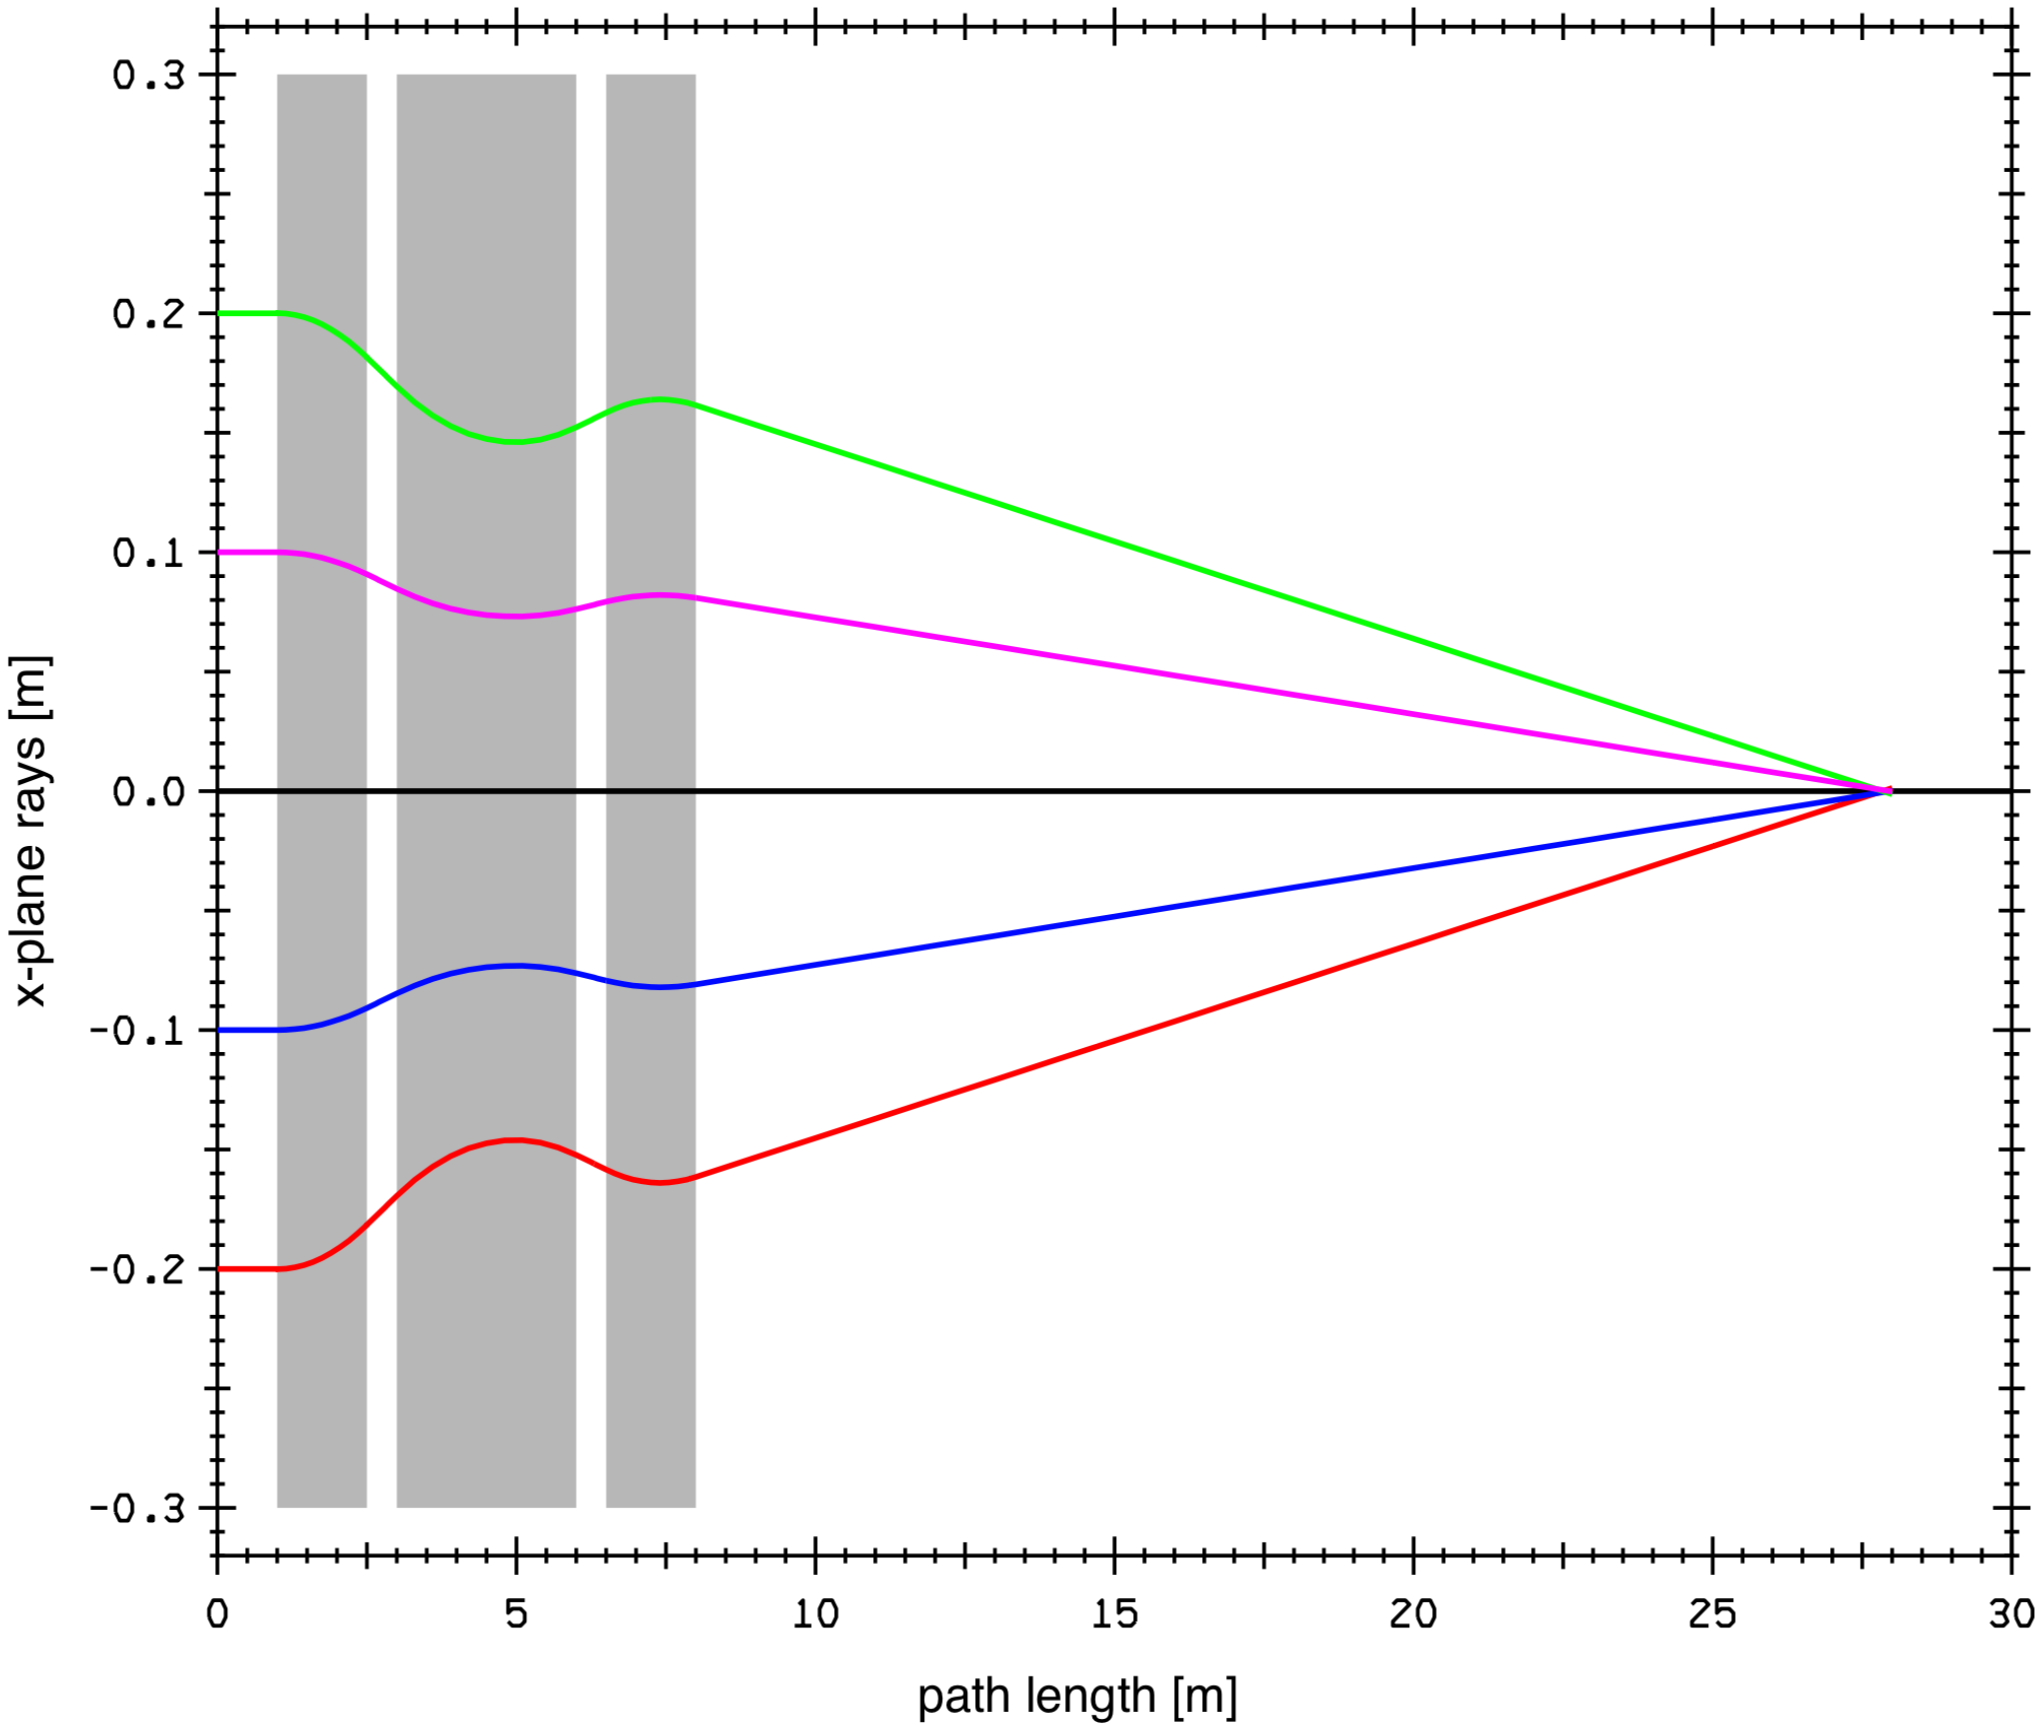
\includegraphics[height=5.75in]{rays}
  \caption{Horizontal plane ray plot for the spot-forming system treated
in section 10.10 accompanied by a schematic showing the lengths and
locations of quadrupoles and their apertures.}
\end{figure}

\newpage
\noindent So doing causes various geometric properties of the spot-forming system to
be computed and written to the external file IFILE, in this case file 40, at
each occurrence of the command {\em dp} (which in turn occurs in the line
{\em \%}).  See section 8.38.  Exhibit 10.12.2c shows the first few lines of file 40.  In
particular, the first column of file 40 is path length along the design orbit.
Finally the {\em merf} command in {\em \#labor} merges the first column of file 40 with the
remaining columns of file 30 and writes the result on file 50.  (See the
contents of {\em \#labor} and section 8.40.)  Exhibit 10.12.2d shows the first few lines of
file 50.  Note that the contents of Exhibits 10.12.2d and 10.10c are identical
except for the interchange of various columns.  Therefore, if desired, this file
could be used to produce (with the aid of any of a variety of graphics programs)
simple ray plots of the form shown in section 10.10.

In addition to file 40 (which contains path-length and coordinate data),
{\em geom} also writes simple element description and path-length information to
the file KFILE, in this case file 60.  See section 8.38.  Exhibit 10.12.2e
shows the first few lines of file 60.  By processing with POSTER simultaneously file
50 (written by {\em merf}) and file 60, it is possible to produce ray plots
accompanied by geometrical information about the associated beam line.
Figure 10.12.2
shows a composite ray plot produced in this way for the spot-forming system of
sections 2.2 and 10.10.  This composite plot displays the lengths,
locations, and apertures of the quadrupoles in the beam line as well as ray data.\index{POSTER}

There is one last detail to be described.  Observe, by comparing Exhibits
10.10f and 10.12.2f, that the lines {\em hfq} and {\em hdq} in this case contain a
{\em dims} command with user name {\em aperture}.  This command is recognized by {\em geom},
affects the contents of the file 60 it writes, and is used to specify the aperture
size for the quadrupoles that appear in figure 10.12.2.  See section 7.40.
\begin{footnotesize}
\begin{verbatim}
Exhibit 10.12.2a
Instructions in file 20 for the sq command:

 1  z(  1,1)
 2  z(  2,1)
 3  z(  3,1)
 4  z(  4,1)
 #


Exhibit 10.12.2b
First few lines of file 30 that contains data written in response
to the wsq command.  In accord with the order presented in Exhibit
10.12.2a, the columns are the horizontal (X) position coordinates
of rays 1 through 4, respectively:

-2.00000E-01  2.00000E-01 -1.00000E-01  1.00000E-01
-2.00000E-01  2.00000E-01 -1.00000E-01  1.00000E-01
-2.00000E-01  2.00000E-01 -1.00000E-01  1.00000E-01
-2.00000E-01  2.00000E-01 -1.00000E-01  1.00000E-01
-2.00000E-01  2.00000E-01 -1.00000E-01  1.00000E-01
-2.00000E-01  2.00000E-01 -1.00000E-01  1.00000E-01
-2.00000E-01  2.00000E-01 -1.00000E-01  1.00000E-01
-2.00000E-01  2.00000E-01 -1.00000E-01  1.00000E-01
-2.00000E-01  2.00000E-01 -1.00000E-01  1.00000E-01
-2.00000E-01  2.00000E-01 -1.00000E-01  1.00000E-01
-2.00000E-01  2.00000E-01 -1.00000E-01  1.00000E-01
-2.00000E-01  2.00000E-01 -1.00000E-01  1.00000E-01
-2.00000E-01  2.00000E-01 -1.00000E-01  1.00000E-01
-2.00000E-01  2.00000E-01 -1.00000E-01  1.00000E-01
-2.00000E-01  2.00000E-01 -1.00000E-01  1.00000E-01
-2.00000E-01  2.00000E-01 -1.00000E-01  1.00000E-01
-2.00000E-01  2.00000E-01 -1.00000E-01  1.00000E-01
-2.00000E-01  2.00000E-01 -1.00000E-01  1.00000E-01
-2.00000E-01  2.00000E-01 -1.00000E-01  1.00000E-01
-2.00000E-01  2.00000E-01 -1.00000E-01  1.00000E-01
-2.00000E-01  2.00000E-01 -1.00000E-01  1.00000E-01
-2.00000E-01  2.00000E-01 -1.00000E-01  1.00000E-01
-2.00056E-01  2.00056E-01 -1.00007E-01  1.00007E-01
-1.99868E-01  1.99868E-01 -9.99132E-02  9.99132E-02
-1.99306E-01  1.99306E-01 -9.96320E-02  9.96320E-02
-1.98369E-01  1.98369E-01 -9.91641E-02  9.91641E-02



Exhibit 10.12.2c
First few lines of file 40 that contains data written in response to
the geom command.  Column 1 is path length along the design orbit:

 0.00000E+00  0.00000E+00  0.00000E+00  0.00000E+00  0.00000E+00  0.00000E+00
 5.00000E-02  0.00000E+00  0.00000E+00  5.00000E-02  5.31071E-10  0.00000E+00
 1.00000E-01  0.00000E+00  0.00000E+00  1.00000E-01  1.06214E-09  0.00000E+00
 1.50000E-01  0.00000E+00  0.00000E+00  1.50000E-01  1.59321E-09  0.00000E+00
 2.00000E-01  0.00000E+00  0.00000E+00  2.00000E-01  2.12429E-09  0.00000E+00
 2.50000E-01  0.00000E+00  0.00000E+00  2.50000E-01  2.65536E-09  0.00000E+00
 3.00000E-01  0.00000E+00  0.00000E+00  3.00000E-01  3.18643E-09  0.00000E+00
 3.50000E-01  0.00000E+00  0.00000E+00  3.50000E-01  3.71750E-09  0.00000E+00
 4.00000E-01  0.00000E+00  0.00000E+00  4.00000E-01  4.24857E-09  0.00000E+00
 4.50000E-01  0.00000E+00  0.00000E+00  4.50000E-01  4.77964E-09  0.00000E+00
 5.00000E-01  0.00000E+00  0.00000E+00  5.00000E-01  5.31071E-09  0.00000E+00
 5.50000E-01  0.00000E+00  0.00000E+00  5.50000E-01  5.84179E-09  0.00000E+00
 6.00000E-01  0.00000E+00  0.00000E+00  6.00000E-01  6.37286E-09  0.00000E+00
 6.50000E-01  0.00000E+00  0.00000E+00  6.50000E-01  6.90393E-09  0.00000E+00
 7.00000E-01  0.00000E+00  0.00000E+00  7.00000E-01  7.43500E-09  0.00000E+00
 7.50000E-01  0.00000E+00  0.00000E+00  7.50000E-01  7.96607E-09  0.00000E+00
 8.00000E-01  0.00000E+00  0.00000E+00  8.00000E-01  8.49714E-09  0.00000E+00
 8.50000E-01  0.00000E+00  0.00000E+00  8.50000E-01  9.02821E-09  0.00000E+00
 9.00000E-01  0.00000E+00  0.00000E+00  9.00000E-01  9.55929E-09  0.00000E+00
 9.50000E-01  0.00000E+00  0.00000E+00  9.50000E-01  1.00904E-08  0.00000E+00
 1.00000E+00  0.00000E+00  0.00000E+00  1.00000E+00  1.06214E-08  0.00000E+00
 1.00000E+00  0.00000E+00  0.00000E+00  1.00000E+00  1.06214E-08  0.00000E+00
 1.00000E+00  0.00000E+00  0.00000E+00  1.00000E+00  1.06214E-08  0.00000E+00
 1.15000E+00  0.00000E+00  0.00000E+00  1.15000E+00  1.22146E-08  0.00000E+00
 1.30000E+00  0.00000E+00  0.00000E+00  1.30000E+00  1.38079E-08  0.00000E+00
 1.45000E+00  0.00000E+00  0.00000E+00  1.45000E+00  1.54011E-08  0.00000E+00


Exhibit 10.12.2d
First few lines of file 50 that contains data written in response to
the merf command.  Column 1 is path length along the design orbit, and
the next 4 columnns are the horizontal position coordinates of the 4 rays:

  0.0000E+00 -0.2000E+00  0.2000E+00 -0.1000E+00  0.1000E+00  0.0000E+00
  0.5000E-01 -0.2000E+00  0.2000E+00 -0.1000E+00  0.1000E+00  0.0000E+00
  0.1000E+00 -0.2000E+00  0.2000E+00 -0.1000E+00  0.1000E+00  0.0000E+00
  0.1500E+00 -0.2000E+00  0.2000E+00 -0.1000E+00  0.1000E+00  0.0000E+00
  0.2000E+00 -0.2000E+00  0.2000E+00 -0.1000E+00  0.1000E+00  0.0000E+00
  0.2500E+00 -0.2000E+00  0.2000E+00 -0.1000E+00  0.1000E+00  0.0000E+00
  0.3000E+00 -0.2000E+00  0.2000E+00 -0.1000E+00  0.1000E+00  0.0000E+00
  0.3500E+00 -0.2000E+00  0.2000E+00 -0.1000E+00  0.1000E+00  0.0000E+00
  0.4000E+00 -0.2000E+00  0.2000E+00 -0.1000E+00  0.1000E+00  0.0000E+00
  0.4500E+00 -0.2000E+00  0.2000E+00 -0.1000E+00  0.1000E+00  0.0000E+00
  0.5000E+00 -0.2000E+00  0.2000E+00 -0.1000E+00  0.1000E+00  0.0000E+00
  0.5500E+00 -0.2000E+00  0.2000E+00 -0.1000E+00  0.1000E+00  0.0000E+00
  0.6000E+00 -0.2000E+00  0.2000E+00 -0.1000E+00  0.1000E+00  0.0000E+00
  0.6500E+00 -0.2000E+00  0.2000E+00 -0.1000E+00  0.1000E+00  0.0000E+00
  0.7000E+00 -0.2000E+00  0.2000E+00 -0.1000E+00  0.1000E+00  0.0000E+00
  0.7500E+00 -0.2000E+00  0.2000E+00 -0.1000E+00  0.1000E+00  0.0000E+00
  0.8000E+00 -0.2000E+00  0.2000E+00 -0.1000E+00  0.1000E+00  0.0000E+00
  0.8500E+00 -0.2000E+00  0.2000E+00 -0.1000E+00  0.1000E+00  0.0000E+00
  0.9000E+00 -0.2000E+00  0.2000E+00 -0.1000E+00  0.1000E+00  0.0000E+00
  0.9500E+00 -0.2000E+00  0.2000E+00 -0.1000E+00  0.1000E+00  0.0000E+00
  0.1000E+01 -0.2000E+00  0.2000E+00 -0.1000E+00  0.1000E+00  0.0000E+00
  0.1000E+01 -0.2000E+00  0.2000E+00 -0.1000E+00  0.1000E+00  0.0000E+00
  0.1000E+01 -0.2001E+00  0.2001E+00 -0.1000E+00  0.1000E+00  0.0000E+00
  0.1150E+01 -0.1999E+00  0.1999E+00 -0.9991E-01  0.9991E-01  0.0000E+00
  0.1300E+01 -0.1993E+00  0.1993E+00 -0.9963E-01  0.9963E-01  0.0000E+00
  0.1450E+01 -0.1984E+00  0.1984E+00 -0.9916E-01  0.9916E-01  0.0000E+00


Exhibit 10.12.2e
First few lines of file 60 that contains data written in response to
the geom command.  It contains simple element description and
path-length information:

drs/10    1  1  0.00000E+00  0.00000E+00  0.00000E+00  0.00000E+00
drs/10    1  1  5.00000E-02  0.00000E+00  0.00000E+00  0.00000E+00
drs/10    1  1  5.00000E-02  0.00000E+00  0.00000E+00  0.00000E+00
drs/10    1  1  1.00000E-01  0.00000E+00  0.00000E+00  0.00000E+00
drs/10    1  1  1.00000E-01  0.00000E+00  0.00000E+00  0.00000E+00
drs/10    1  1  1.50000E-01  0.00000E+00  0.00000E+00  0.00000E+00
drs/10    1  1  1.50000E-01  0.00000E+00  0.00000E+00  0.00000E+00
drs/10    1  1  2.00000E-01  0.00000E+00  0.00000E+00  0.00000E+00
drs/10    1  1  2.00000E-01  0.00000E+00  0.00000E+00  0.00000E+00
drs/10    1  1  2.50000E-01  0.00000E+00  0.00000E+00  0.00000E+00
drs/10    1  1  2.50000E-01  0.00000E+00  0.00000E+00  0.00000E+00
drs/10    1  1  3.00000E-01  0.00000E+00  0.00000E+00  0.00000E+00
drs/10    1  1  3.00000E-01  0.00000E+00  0.00000E+00  0.00000E+00
drs/10    1  1  3.50000E-01  0.00000E+00  0.00000E+00  0.00000E+00
drs/10    1  1  3.50000E-01  0.00000E+00  0.00000E+00  0.00000E+00
drs/10    1  1  4.00000E-01  0.00000E+00  0.00000E+00  0.00000E+00
drs/10    1  1  4.00000E-01  0.00000E+00  0.00000E+00  0.00000E+00
drs/10    1  1  4.50000E-01  0.00000E+00  0.00000E+00  0.00000E+00
drs/10    1  1  4.50000E-01  0.00000E+00  0.00000E+00  0.00000E+00
drs/10    1  1  5.00000E-01  0.00000E+00  0.00000E+00  0.00000E+00
drs/10    1  1  5.00000E-01  0.00000E+00  0.00000E+00  0.00000E+00
drs/10    1  1  5.50000E-01  0.00000E+00  0.00000E+00  0.00000E+00
drs/10    1  1  5.50000E-01  0.00000E+00  0.00000E+00  0.00000E+00
drs/10    1  1  6.00000E-01  0.00000E+00  0.00000E+00  0.00000E+00
drs/10    1  1  6.00000E-01  0.00000E+00  0.00000E+00  0.00000E+00
drs/10    1  1  6.50000E-01  0.00000E+00  0.00000E+00  0.00000E+00
drs/10    1  1  6.50000E-01  0.00000E+00  0.00000E+00  0.00000E+00
drs/10    1  1  7.00000E-01  0.00000E+00  0.00000E+00  0.00000E+00
drs/10    1  1  7.00000E-01  0.00000E+00  0.00000E+00  0.00000E+00
drs/10    1  1  7.50000E-01  0.00000E+00  0.00000E+00  0.00000E+00
drs/10    1  1  7.50000E-01  0.00000E+00  0.00000E+00  0.00000E+00
drs/10    1  1  8.00000E-01  0.00000E+00  0.00000E+00  0.00000E+00
drs/10    1  1  8.00000E-01  0.00000E+00  0.00000E+00  0.00000E+00
drs/10    1  1  8.50000E-01  0.00000E+00  0.00000E+00  0.00000E+00
drs/10    1  1  8.50000E-01  0.00000E+00  0.00000E+00  0.00000E+00
drs/10    1  1  9.00000E-01  0.00000E+00  0.00000E+00  0.00000E+00
drs/10    1  1  9.00000E-01  0.00000E+00  0.00000E+00  0.00000E+00
drs/10    1  1  9.50000E-01  0.00000E+00  0.00000E+00  0.00000E+00
drs/10    1  1  9.50000E-01  0.00000E+00  0.00000E+00  0.00000E+00
drs/10    1  1  1.00000E+00  0.00000E+00  0.00000E+00  0.00000E+00
inhfq     1  9  1.00000E+00  3.00000E-01  0.00000E+00  8.63000E-02
hfq/10    1  9  1.00000E+00  3.00000E-01  0.00000E+00  8.63000E-02
hfq/10    1  9  1.15000E+00  3.00000E-01  0.00000E+00  8.63000E-02
hfq/10    1  9  1.15000E+00  3.00000E-01  0.00000E+00  8.63000E-02
hfq/10    1  9  1.30000E+00  3.00000E-01  0.00000E+00  8.63000E-02
hfq/10    1  9  1.30000E+00  3.00000E-01  0.00000E+00  8.63000E-02
hfq/10    1  9  1.45000E+00  3.00000E-01  0.00000E+00  8.63000E-02
hfq/10    1  9  1.45000E+00  3.00000E-01  0.00000E+00  8.63000E-02


Exhibit 10.12.2f
***MARYLIE 3.0***
Prerelease Development Version 6/17/99
Copyright 1987 Alex J. Dragt
All rights reserved

Data input complete; going into #labor.
#comment
 Exhibit 10.12.2
      This is a MARYLIE run that demonstrates the production of ray and
 geometric data for the simple spot forming system of Section 2.2.
 To do this all quads and drifts are split in 10 pieces, except for the
 final long drift which is split in 20 pieces.  The system is also slightly
 modified by preceding it with 2 short drifts.

 The beam parameters are those for 50 MeV protons.

#beam
  1.03527440851950
 5.328901960570000E-002
  1.00000000000000
  1.00000000000000
#menu
 cdrs     drft
  0.500000000000000
 cdrl     drft
   20.0026000000000
 chfq     quad
   1.50000000000000      8.630000000000000E-02   1.00000000000000
   1.00000000000000
 chdq     quad
   3.00000000000000     -8.289450000000000E-02   1.00000000000000
   1.00000000000000
 drs/10   drft
  5.000000000000000E-02
 drl/20   drft
   1.00013000000000
 inhfq    quad
  0.000000000000000E+00  8.630000000000000E-02   1.00000000000000
  0.000000000000000E+00
 outhfq   quad
  0.000000000000000E+00  8.630000000000000E-02  0.000000000000000E+00
   1.00000000000000
 inhdq    quad
  0.000000000000000E+00 -8.289450000000000E-02   1.00000000000000
  0.000000000000000E+00
 outhdq   quad
  0.000000000000000E+00 -8.289450000000000E-02  0.000000000000000E+00
   1.00000000000000
 hfq/10   quad
  0.150000000000000      8.630000000000000E-02  0.000000000000000E+00
  0.000000000000000E+00
 hdq/10   quad
  0.300000000000000     -8.289450000000000E-02  0.000000000000000E+00
  0.000000000000000E+00
 aperture dims
  0.300000000000000      0.000000000000000E+00  0.000000000000000E+00
  0.000000000000000E+00  0.000000000000000E+00  0.000000000000000E+00
 fileout  pmif
   1.00000000000000       12.0000000000000       3.00000000000000
 mapout   ptm
   3.00000000000000       3.00000000000000      0.000000000000000E+00
  0.000000000000000E+00   1.00000000000000
 inv      inv
 wcl10    wcl
   3.00000000000000       10.0000000000000       3.00000000000000
 mark     mark
 iden     iden
 raysin   rt
   13.0000000000000       14.0000000000000      -1.00000000000000
  0.000000000000000E+00  0.000000000000000E+00  0.000000000000000E+00
 rt       rt
  0.000000000000000E+00   14.0000000000000       5.00000000000000
   1.00000000000000       1.00000000000000      0.000000000000000E+00
 sq       sq
   20.0000000000000      0.000000000000000E+00   1.00000000000000
   1.00000000000000
 wsq      wsq
   1.00000000000000       1.00000000000000       30.0000000000000
   1.00000000000000       2.00000000000000      0.000000000000000E+00
 dp       dp
 geom     geom
   3.00000000000000      0.000000000000000E+00  0.000000000000000E+00
   1.00000000000000       2.00000000000000      0.000000000000000E+00
 ps1      ps1
  0.000000000000000E+00  0.000000000000000E+00  0.000000000000000E+00
  0.000000000000000E+00  0.000000000000000E+00  0.000000000000000E+00
 ps2      ps2
   40.0000000000000      0.000000000000000E+00   60.0000000000000
  0.000000000000000E+00  0.000000000000000E+00   1.00000000000000
 merf     usr12
   40.0000000000000       30.0000000000000       50.0000000000000
   1.00000000000000       4.00000000000000      0.000000000000000E+00
 end      end
#lines
 hfq
     1*aperture    1*inhfq      10*hfq/10      1*outhfq
 hdq
     1*aperture    1*inhdq      10*hdq/10      1*outhdq
 drs
    10*drs/10
 drl
    20*drl/20
 trip
     1*hfq         1*drs         1*hdq         1*drs         1*hfq
 spot
     2*drs         1*trip        1*drl
 ctrip
     1*chfq        1*cdrs        1*chdq        1*cdrs        1*chfq
 cspot
     2*cdrs        1*ctrip       1*cdrl
 %spot
     1*%           1*drs/10      1*%           1*drs/10      1*%        &
     1*drs/10      1*%           1*drs/10      1*%           1*drs/10   &
     1*%           1*drs/10      1*%           1*drs/10      1*%        &
     1*drs/10      1*%           1*drs/10      1*%           1*drs/10   &
     1*%           1*drs/10      1*%           1*drs/10      1*%        &
     1*drs/10      1*%           1*drs/10      1*%           1*drs/10   &
     1*%           1*drs/10      1*%           1*drs/10      1*%        &
     1*drs/10      1*%           1*drs/10      1*%           1*drs/10   &
     1*%           1*aperture    1*%           1*inhfq       1*%        &
     1*hfq/10      1*%           1*hfq/10      1*%           1*hfq/10   &
     1*%           1*hfq/10      1*%           1*hfq/10      1*%        &
     1*hfq/10      1*%           1*hfq/10      1*%           1*hfq/10   &
     1*%           1*hfq/10      1*%           1*hfq/10      1*%        &
     1*outhfq      1*%           1*drs/10      1*%           1*drs/10   &
     1*%           1*drs/10      1*%           1*drs/10      1*%        &
     1*drs/10      1*%           1*drs/10      1*%           1*drs/10   &
     1*%           1*drs/10      1*%           1*drs/10      1*%        &
     1*drs/10      1*%           1*aperture    1*%           1*inhdq    &
     1*%           1*hdq/10      1*%           1*hdq/10      1*%        &
     1*hdq/10      1*%           1*hdq/10      1*%           1*hdq/10   &
     1*%           1*hdq/10      1*%           1*hdq/10      1*%        &
     1*hdq/10      1*%           1*hdq/10      1*%           1*hdq/10   &
     1*%           1*outhdq      1*%           1*drs/10      1*%        &
     1*drs/10      1*%           1*drs/10      1*%           1*drs/10   &
     1*%           1*drs/10      1*%           1*drs/10      1*%        &
     1*drs/10      1*%           1*drs/10      1*%           1*drs/10   &
     1*%           1*drs/10      1*%           1*aperture    1*%        &
     1*inhfq       1*%           1*hfq/10      1*%           1*hfq/10   &
     1*%           1*hfq/10      1*%           1*hfq/10      1*%        &
     1*hfq/10      1*%           1*hfq/10      1*%           1*hfq/10   &
     1*%           1*hfq/10      1*%           1*hfq/10      1*%        &
     1*hfq/10      1*%           1*outhfq      1*%           1*drl/20   &
     1*%           1*drl/20      1*%           1*drl/20      1*%        &
     1*drl/20      1*%           1*drl/20      1*%           1*drl/20   &
     1*%           1*drl/20      1*%           1*drl/20      1*%        &
     1*drl/20      1*%           1*drl/20      1*%           1*drl/20   &
     1*%           1*drl/20      1*%           1*drl/20      1*%        &
     1*drl/20      1*%           1*drl/20      1*%           1*drl/20   &
     1*%           1*drl/20      1*%           1*drl/20      1*%        &
     1*drl/20      1*%           1*drl/20      1*%
 %
     1*work        1*dp
 work
     1*rt          1*wsq         1*iden
 setup
     1*raysin      1*sq
 cgeom
     1*ps1         1*ps2         1*geom
#lumps
#loops
 lspot
     1*spot
 l%spot
     1*%spot
#labor
    1*fileout
    1*setup
    1*%spot
    1*l%spot
    1*cgeom
    1*merf
    1*end

*******************************
* Response to raysin command: *
*******************************

    4 ray(s) read in from file  13

*******************************
* Response to the command sq: *
*******************************

 In subroutine sq
accept  1:    z(  1,1)
accept  2:    z(  2,1)
accept  3:    z(  3,1)
accept  4:    z(  4,1)

 Aims/quantities selected :
No.     item      present value
----------------------------------
 1  z(  1,1) =     -0.200000000
 2  z(  2,1) =      0.200000000
 3  z(  3,1) =     -0.100000000
 4  z(  4,1) =      0.100000000

*****************************
* Response to merf command: *
*****************************

 number of lines read =         100

end of MARYLIE run
\end{verbatim}
\end{footnotesize}

\newpage
\subsection{Beam Moment Plots with Geometry}\index{beam moment plots with geometry} \index{geometry} \index{plots} \index{moment}
\label{beammomplots}
Figure 10.12.3.1 shows a position spread plot, with additional geometric data, for the
spot-forming system of sections 2.2 and 10.11.  Exhibit 10.12.3f shows
the \Mary run used to produce this plot.  Much of this Master Input File
is similar to that of Exhibit 10.11c.  However, there are a few
differences that are described below.

First, because path-length information will now be provided by {\em
geom}, file 20 which provides instruction for {\em sq} is shortened to
exclude {\em pl} as shown in Exhibit 10.12.3a.  Correspondingly, as shown
in Exhibit 10.12.3b, file 30 now contains only spread and moment
quantities.

Second, the line {\em \%} now takes the form
\begin{footnotesize}
\begin{verbatim}
%
     1*work1     1*dp
\end{verbatim}
\end{footnotesize}
and the line {\em work1} itself takes the  simpler form
\begin{footnotesize}
\begin{verbatim}
work1
     1*samap     1*wsq
\end{verbatim}
\end{footnotesize}
since there is now no need to invoke a {\em pli0} command because
path-length information will be computed by {\em geom}.

Third, the {\em \#labor} component of the Master Input File now has the
contents
\begin{footnotesize}
\begin{verbatim}
#labor
	 1*fileout
	 1*setup1
	 1*%spot
	 1*l%spot
	 1*cgeom
	 1*merf
	 1*end
\end{verbatim}
\end{footnotesize}
The first 3 entries ({\em 1*fileout}, {\em 1*setup1}, {\em 1*\%spot}) function as before
except that (as already mentioned) only spead and moment, and not path-length,
information is written on file 30.  See Exhibit 10.12.3b.  The entry
{\em 1*l\%spot} invokes a loop whose contents is {\em \%spot}.  See the
{\em \#loops} component of
Exhibit 10.12.3f.  The entry {\em cgeom} invokes a line that contains a {\em geom} command
preceded by the commands {\em ps1} and {\em ps2} that set the parameters required by geom:
\begin{footnotesize}
\begin{verbatim}
cgeom
     1*ps1   1*ps2  1*geom
\end{verbatim}
\end{footnotesize}

\newpage
\begin{figure}[htp]
\setcounter{figure}{0}
  \centering
  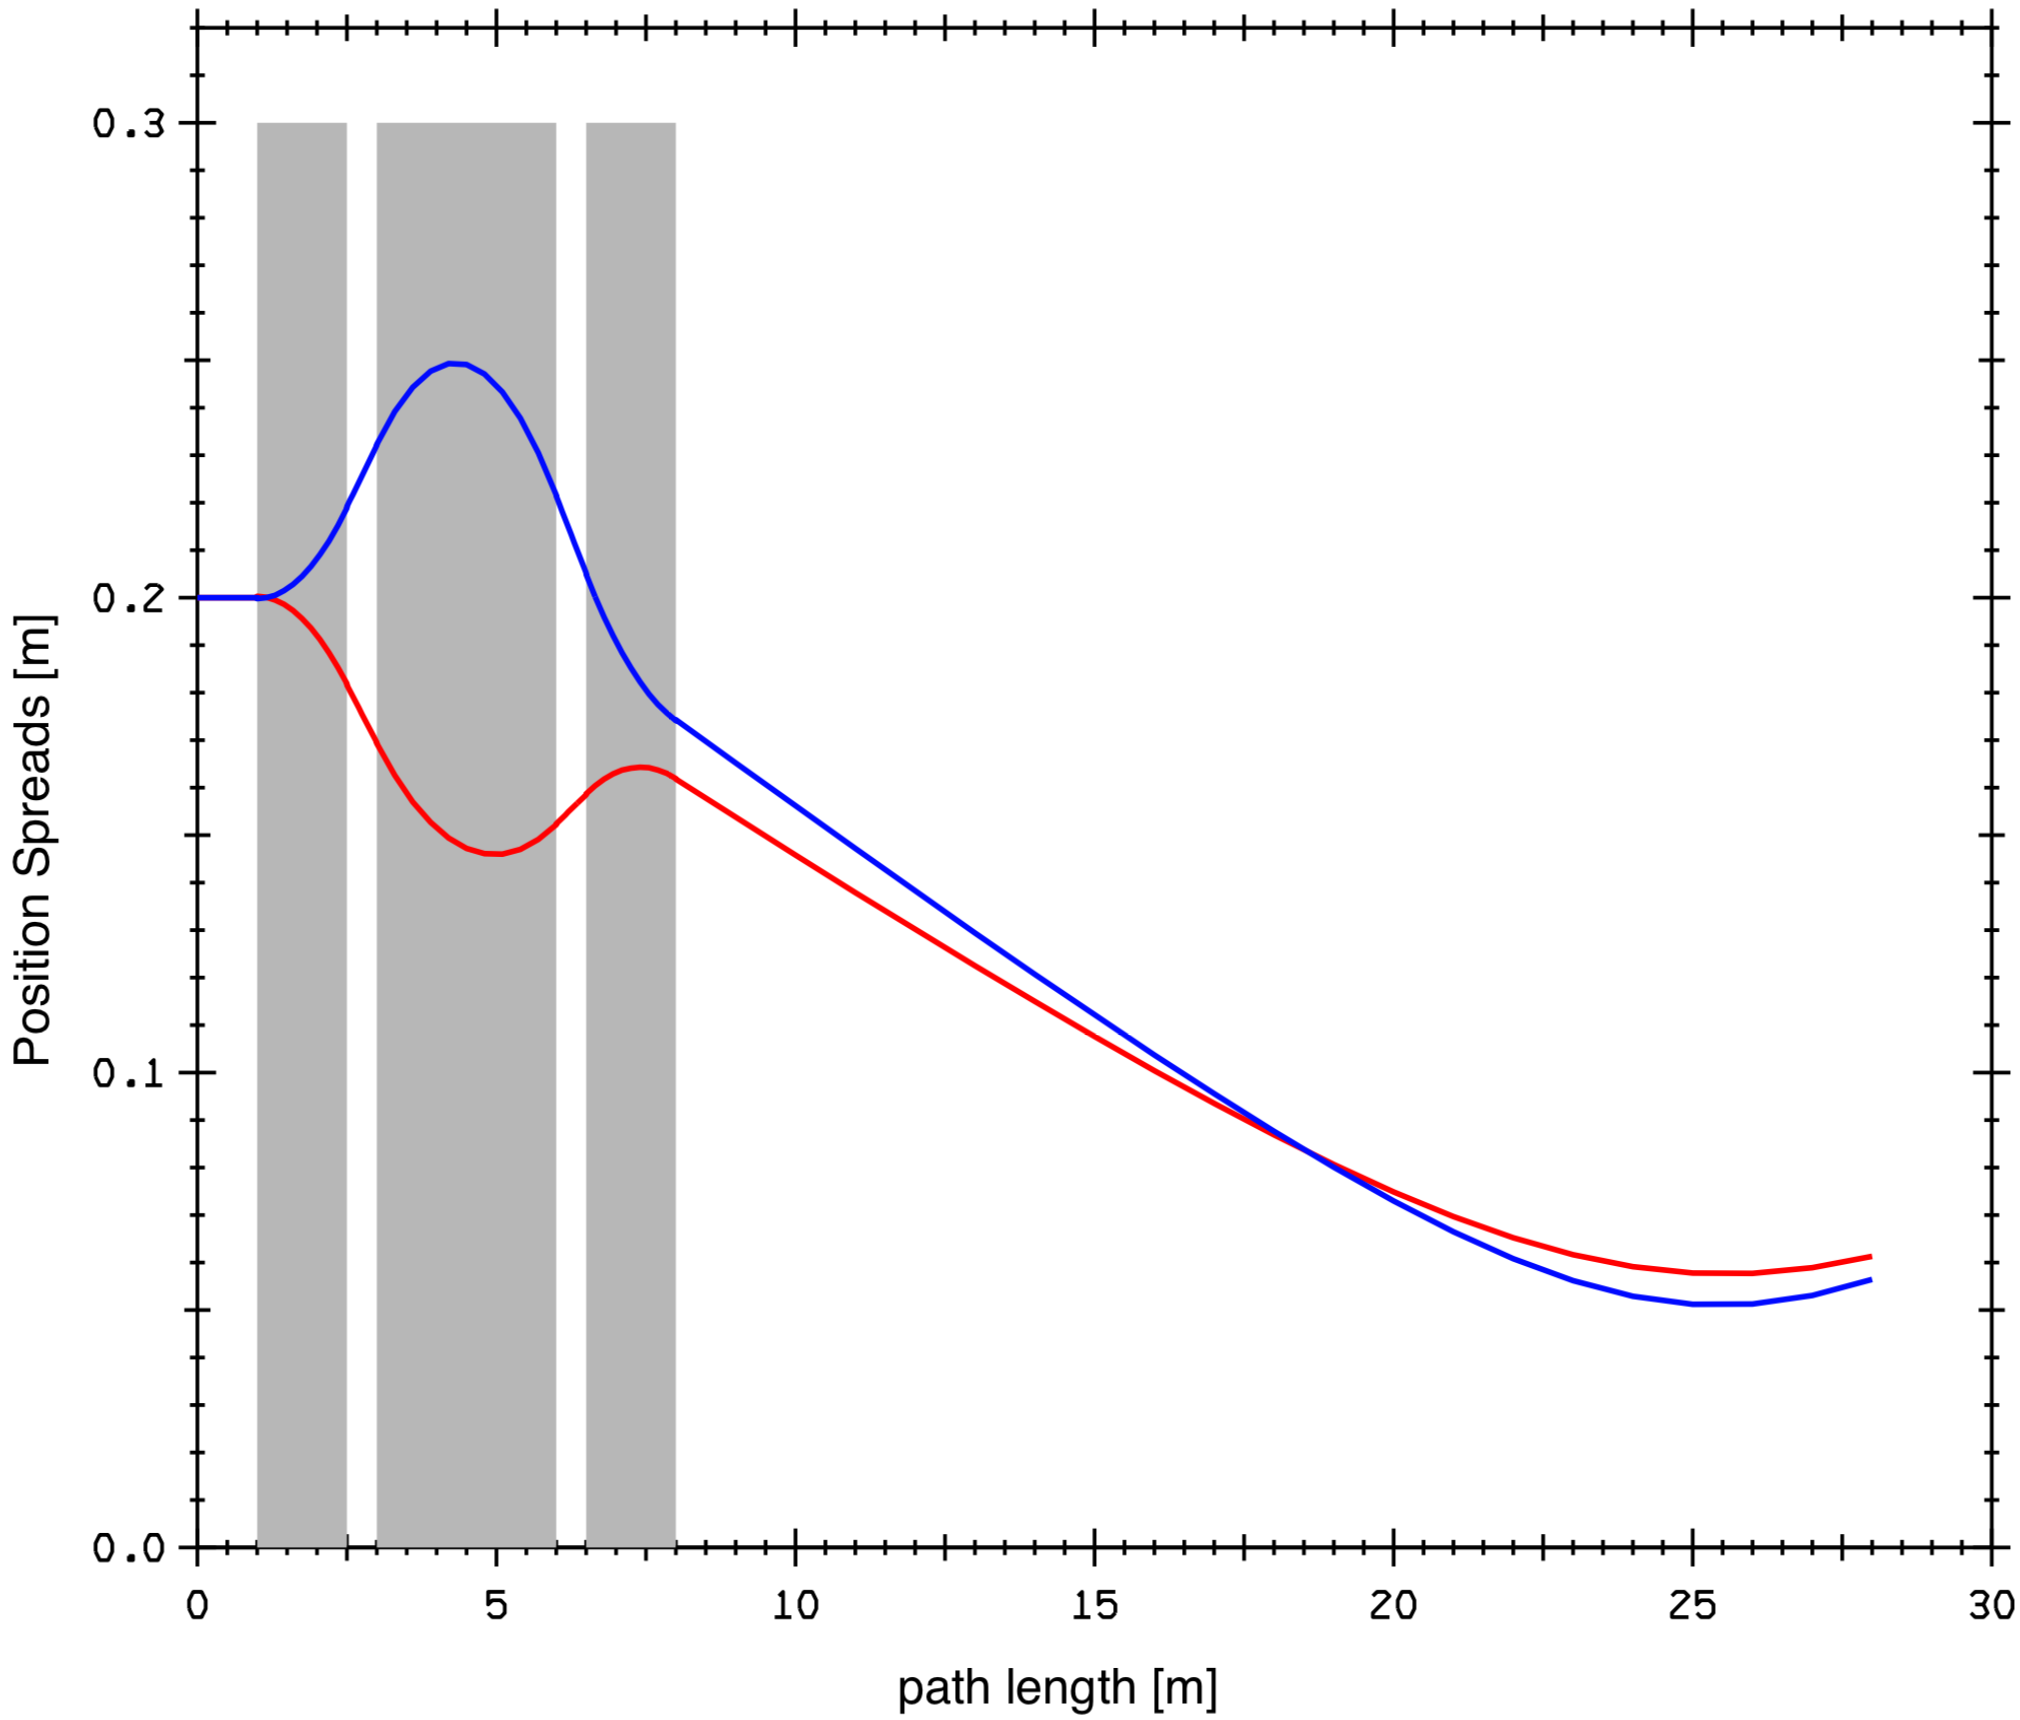
\includegraphics[height=5.75in]{mom1}
  \caption{The rms position spreads $\sqrt{\langle X^2\rangle}$ and
$\sqrt{\langle Y^2\rangle}$ for the
spot-forming system treated in section 10.11 accompanied by a schematic
showing the lengths and locations of quadrupoles and their apertures.}
\end{figure}

\newpage
\noindent So doing causes various geometric properties of the spot-forming system to
be computed and written to the external file IFILE, in this case file 40, at each
occurrence of the command {\em dp} (which in turn occurs in the line \%).  See
section 8.38.  Exhibit 10.12.3c shows the first few lines of file 40.  In
particular, the first column of file 40 is path length along the design orbit.
Finally the {\em merf} command in {\em \#labor} merges the first column of file 40 with the
remaining columns of file 30 and writes the result on file 50.  (See the contents of
{\em \#labor} and section 8.40.)  Exhibit 10.12.3d shows the first few lines of
file 50.  Note that the contents of Exhibits 10.12.3d and 10.11b are identical
except for the interchange of various columns.  Therefore, if desired, this file
could be used to produce (with the aid of any of a variety of graphics programs)
simple spread and moment plots of the form shown in section 10.11.

In addition to file 40 (which contains path-length and coordinate data),
{\em geom} also writes simple element description and path-length information to
the file KFILE, in this case file 60.  See section 8.38.  Exhibit 10.12.3e
shows the first few lines of file 60.  By processing with POSTER simultaneously file
50 (written by {\em merf}) and file 60, it is possible to produce spread and moment
plots accompanied by geometrical information about the associated beam line.
Figure 10.12.3 shows a composite spread  plot produced in this way for the
spot-forming system of sections 2.2 and 10.11.  This composite plot displays the
lengths, locations, and apertures of the quadrupoles in the beam line as well as
spread data.\index{POSTER}

There is one last detail to be described.  Observe, by comparing Exhibits
10.11c and 10.12.3f, that the lines {\em hfq} and {\em hdq} in this case contain a
{\em dims} command with user name {\em aperture}.  This command is recognized by {\em geom},
affects the contents of the file 60 it writes, and is used to specify the aperture
size for the quadrupoles that appear in figure 10.12.3.  See section 7.40.
\begin{footnotesize}
\begin{verbatim}
Exhibit 10.12.3a
Instructions in file 20 for the sq command:

 1  bm2(1,1)
 2  bm2(2,2)
 3  bm2(3,3)
 4  bm2(4,4)
 5  bm1(1,2)
 #


Exhibit 10.12.3b
First few lines of file 30 that contains data written in response to the
wsq command.  In accord with the ordering specified in Exhibit 10.12a
above, the columns are the spread and moment quantities sqrt<XX>,
sqrt<PxPx>, sqrt<YY>, sqrt<PyPy>, and <XPx>, respectively.

 2.00000E-01  2.50000E-03  2.00000E-01  2.50000E-03  0.00000E+00
 2.00000E-01  2.50000E-03  2.00000E-01  2.50000E-03  3.12503E-07
 2.00000E-01  2.50000E-03  2.00000E-01  2.50000E-03  6.25006E-07
 2.00000E-01  2.50000E-03  2.00000E-01  2.50000E-03  9.37509E-07
 2.00001E-01  2.50000E-03  2.00001E-01  2.50000E-03  1.25001E-06


Exhibit 10.12.3c
First few lines of file 40 that contains data written in response to
the geom command.  Column 1 is path length data along the design orbit:

 0.00000E+00  0.00000E+00  0.00000E+00  0.00000E+00  0.00000E+00  0.00000E+00
 5.00000E-02  0.00000E+00  0.00000E+00  5.00000E-02  5.31071E-10  0.00000E+00
 1.00000E-01  0.00000E+00  0.00000E+00  1.00000E-01  1.06214E-09  0.00000E+00
 1.50000E-01  0.00000E+00  0.00000E+00  1.50000E-01  1.59321E-09  0.00000E+00
 2.00000E-01  0.00000E+00  0.00000E+00  2.00000E-01  2.12429E-09  0.00000E+00


Exhibit 10.12.3d
First few lines of file 40 that contains data written in response to
the merf command.  Column 1 is path length data along the design orbit,
and the next 4 columns are spread and moment quantities:

  0.0000E+00  0.2000E+00  0.2500E-02  0.2000E+00  0.2500E-02  0.0000E+00
  0.5000E-01  0.2000E+00  0.2500E-02  0.2000E+00  0.2500E-02  0.3125E-06
  0.1000E+00  0.2000E+00  0.2500E-02  0.2000E+00  0.2500E-02  0.6250E-06
  0.1500E+00  0.2000E+00  0.2500E-02  0.2000E+00  0.2500E-02  0.9375E-06
  0.2000E+00  0.2000E+00  0.2500E-02  0.2000E+00  0.2500E-02  0.1250E-05


Exhibit 10.12.3e
First few lines of file 60 that contains data written in response to
the geom command.  It contains simple element description and
path-length information:

drs/10    1  1  0.00000E+00  0.00000E+00  0.00000E+00  0.00000E+00
drs/10    1  1  5.00000E-02  0.00000E+00  0.00000E+00  0.00000E+00
drs/10    1  1  5.00000E-02  0.00000E+00  0.00000E+00  0.00000E+00
drs/10    1  1  1.00000E-01  0.00000E+00  0.00000E+00  0.00000E+00
drs/10    1  1  1.00000E-01  0.00000E+00  0.00000E+00  0.00000E+00
drs/10    1  1  1.50000E-01  0.00000E+00  0.00000E+00  0.00000E+00
drs/10    1  1  1.50000E-01  0.00000E+00  0.00000E+00  0.00000E+00
drs/10    1  1  2.00000E-01  0.00000E+00  0.00000E+00  0.00000E+00
drs/10    1  1  2.00000E-01  0.00000E+00  0.00000E+00  0.00000E+00


Exhibit 10.12.3f
***MARYLIE 3.0***
Prerelease Development Version 6/17/99
Copyright 1987 Alex J. Dragt
All rights reserved

Data input complete; going into #labor.
#comment
 Exhibit 10.12.3
      This is a MARYLIE run that demonstrates the production of beam moment
 and geometric data for the simple spot forming system of Section 2.2.
 To do this all quads and drifts are split in 10 pieces, except for the
 final long drift  which is split in 20 pieces.  The system is also
 slightly modified by preceding it with 2 short drifts.

 Transformed moments are computed from the initial moments using the
 accumulated transfer map.  See the contents of the line work1.

 Alternatively, transformed moments could be computed from the
 moments just preceding using just the map for the current element
 slice.  See the contents of the line work2.  This approach is the
 "moment" analog of element-by-element (actually slice-by-slice)
 tracking.

 The beam parameters are those for 50 MeV protons.

#beam
  1.03527440851950
 5.328901960570000E-002
  1.00000000000000
  1.00000000000000
#menu
 cdrs     drft
  0.500000000000000
 cdrl     drft
   20.0026000000000
 chfq     quad
   1.50000000000000      8.630000000000000E-02   1.00000000000000
   1.00000000000000
 chdq     quad
   3.00000000000000     -8.289450000000000E-02   1.00000000000000
   1.00000000000000
 drs/10   drft
  5.000000000000000E-02
 drl/20   drft
   1.00013000000000
 inhfq    quad
  0.000000000000000E+00  8.630000000000000E-02   1.00000000000000
  0.000000000000000E+00
 outhfq   quad
  0.000000000000000E+00  8.630000000000000E-02  0.000000000000000E+00
   1.00000000000000
 inhdq    quad
  0.000000000000000E+00 -8.289450000000000E-02   1.00000000000000
  0.000000000000000E+00
 outhdq   quad
  0.000000000000000E+00 -8.289450000000000E-02  0.000000000000000E+00
   1.00000000000000
 hfq/10   quad
  0.150000000000000      8.630000000000000E-02  0.000000000000000E+00
  0.000000000000000E+00
 hdq/10   quad
  0.300000000000000     -8.289450000000000E-02  0.000000000000000E+00
  0.000000000000000E+00
 aperture dims
  0.300000000000000      0.000000000000000E+00  0.000000000000000E+00
  0.000000000000000E+00  0.000000000000000E+00  0.000000000000000E+00
 fileout  pmif
   1.00000000000000       12.0000000000000       3.00000000000000
 mapout   ptm
   3.00000000000000       3.00000000000000      0.000000000000000E+00
  0.000000000000000E+00   1.00000000000000
 inv      inv
 wcl10    wcl
   3.00000000000000       10.0000000000000       3.00000000000000
 mark     mark
 iden     iden
 raysin   rt
   13.0000000000000       14.0000000000000      -1.00000000000000
  0.000000000000000E+00  0.000000000000000E+00  0.000000000000000E+00
 rt       rt
  0.000000000000000E+00   14.0000000000000       5.00000000000000
   1.00000000000000       1.00000000000000      0.000000000000000E+00
 sq       sq
   20.0000000000000      0.000000000000000E+00   1.00000000000000
   1.00000000000000
 wsq      wsq
   1.00000000000000       1.00000000000000       30.0000000000000
   1.00000000000000       2.00000000000000      0.000000000000000E+00
 dp       dp
 geom     geom
   3.00000000000000      0.000000000000000E+00  0.000000000000000E+00
   1.00000000000000       2.00000000000000      0.000000000000000E+00
 ps1      ps1
  0.000000000000000E+00  0.000000000000000E+00  0.000000000000000E+00
  0.000000000000000E+00  0.000000000000000E+00  0.000000000000000E+00
 ps2      ps2
   40.0000000000000      0.000000000000000E+00   60.0000000000000
  0.000000000000000E+00  0.000000000000000E+00   1.00000000000000
 merf     usr12
   40.0000000000000       30.0000000000000       50.0000000000000
   1.00000000000000       5.00000000000000      0.000000000000000E+00
 bgen     bgen
   2.00000000000000       2.00000000000000      0.000000000000000E+00
   123.000000000000       1.00000000000000       3.00000000000000
 ps3      ps3
  5.000000000000000E-04  5.000000000000000E-04  0.000000000000000E+00
  0.000000000000000E+00  0.000000000000000E+00  0.000000000000000E+00
 gbuf1    gbuf
   2.00000000000000       1.00000000000000
 gbuf2    gbuf
   2.00000000000000       2.00000000000000
 twx      twsm
   1.00000000000000       86.0000000000000      0.000000000000000E+00
   80.0000000000000
 twy      twsm
   2.00000000000000       96.0000000000000      0.000000000000000E+00
   80.0000000000000
 amap     amap
   2.00000000000000       1.00000000000000      -1.00000000000000
  0.000000000000000E+00  0.000000000000000E+00  0.000000000000000E+00
 samap    amap
   2.00000000000000      0.000000000000000E+00  -1.00000000000000
  0.000000000000000E+00  0.000000000000000E+00  0.000000000000000E+00
 stm1     stm
   1.00000000000000
 snor     snor
  0.000000000000000E+00  0.000000000000000E+00  0.000000000000000E+00
  0.000000000000000E+00  0.000000000000000E+00
 end      end
#lines
 hfq
     1*aperture    1*inhfq      10*hfq/10      1*outhfq
 hdq
     1*aperture    1*inhdq      10*hdq/10      1*outhdq
 drs
    10*drs/10
 drl
    20*drl/20
 trip
     1*hfq         1*drs         1*hdq         1*drs         1*hfq
 spot
     2*drs         1*trip        1*drl
 ctrip
     1*chfq        1*cdrs        1*chdq        1*cdrs        1*chfq
 cspot
     2*cdrs        1*ctrip       1*cdrl
 %spot
     1*%           1*drs/10      1*%           1*drs/10      1*%        &
     1*drs/10      1*%           1*drs/10      1*%           1*drs/10   &
     1*%           1*drs/10      1*%           1*drs/10      1*%        &
     1*drs/10      1*%           1*drs/10      1*%           1*drs/10   &
     1*%           1*drs/10      1*%           1*drs/10      1*%        &
     1*drs/10      1*%           1*drs/10      1*%           1*drs/10   &
     1*%           1*drs/10      1*%           1*drs/10      1*%        &
     1*drs/10      1*%           1*drs/10      1*%           1*drs/10   &
     1*%           1*aperture    1*%           1*inhfq       1*%        &
     1*hfq/10      1*%           1*hfq/10      1*%           1*hfq/10   &
     1*%           1*hfq/10      1*%           1*hfq/10      1*%        &
     1*hfq/10      1*%           1*hfq/10      1*%           1*hfq/10   &
     1*%           1*hfq/10      1*%           1*hfq/10      1*%        &
     1*outhfq      1*%           1*drs/10      1*%           1*drs/10   &
     1*%           1*drs/10      1*%           1*drs/10      1*%        &
     1*drs/10      1*%           1*drs/10      1*%           1*drs/10   &
     1*%           1*drs/10      1*%           1*drs/10      1*%        &
     1*drs/10      1*%           1*aperture    1*%           1*inhdq    &
     1*%           1*hdq/10      1*%           1*hdq/10      1*%        &
     1*hdq/10      1*%           1*hdq/10      1*%           1*hdq/10   &
     1*%           1*hdq/10      1*%           1*hdq/10      1*%        &
     1*hdq/10      1*%           1*hdq/10      1*%           1*hdq/10   &
     1*%           1*outhdq      1*%           1*drs/10      1*%        &
     1*drs/10      1*%           1*drs/10      1*%           1*drs/10   &
     1*%           1*drs/10      1*%           1*drs/10      1*%        &
     1*drs/10      1*%           1*drs/10      1*%           1*drs/10   &
     1*%           1*drs/10      1*%           1*aperture    1*%        &
     1*inhfq       1*%           1*hfq/10      1*%           1*hfq/10   &
     1*%           1*hfq/10      1*%           1*hfq/10      1*%        &
     1*hfq/10      1*%           1*hfq/10      1*%           1*hfq/10   &
     1*%           1*hfq/10      1*%           1*hfq/10      1*%        &
     1*hfq/10      1*%           1*outhfq      1*%           1*drl/20   &
     1*%           1*drl/20      1*%           1*drl/20      1*%        &
     1*drl/20      1*%           1*drl/20      1*%           1*drl/20   &
     1*%           1*drl/20      1*%           1*drl/20      1*%        &
     1*drl/20      1*%           1*drl/20      1*%           1*drl/20   &
     1*%           1*drl/20      1*%           1*drl/20      1*%        &
     1*drl/20      1*%           1*drl/20      1*%           1*drl/20   &
     1*%           1*drl/20      1*%           1*drl/20      1*%        &
     1*drl/20      1*%           1*drl/20      1*%
 %
     1*work1       1*dp
 work1
     1*samap       1*wsq
 work2
     1*samap       1*wsq         1*gbuf1       1*stm1        1*iden
 setup
     1*momgen      1*sq
 momgen
     1*ps3         1*bgen        1*gbuf2       1*mapout      1*stm1     &
     1*iden        1*tws         1*mapout      1*snor        1*gbuf1    &
     1*mapout      1*amap        1*gbuf1       1*mapout      1*stm1     &
     1*iden
 tws
     1*twx         1*twy
 cgeom
     1*ps1         1*ps2         1*geom
#lumps
#loops
 lspot
     1*spot
 l%spot
     1*%spot
#labor
    1*fileout
    1*setup
    1*%spot
    1*l%spot
    1*cgeom
    1*merf
    1*end

*********************************
* Response to the command bgen: *
*********************************

 analytically computed values of selected moments
 values of <x*x>, <x*px>, <px*px>:
 5.000000000000000E-004  0.000000000000000E+000  5.000000000000000E-004
 values of <y*y>, <y*py>, <py*py>:
 5.000000000000000E-004  0.000000000000000E+000  5.000000000000000E-004
 values of <t*t>, <t*pt>, <pt*pt>:
 0.000000000000000E+000  0.000000000000000E+000  0.000000000000000E+000

*********************************************
* Moments written in "map" form in response *
* to the gbuf2 and mapout commands:         *
*********************************************

matrix for map is :

 5.00000E-04  0.00000E+00  0.00000E+00  0.00000E+00  0.00000E+00  0.00000E+00
 0.00000E+00  5.00000E-04  0.00000E+00  0.00000E+00  0.00000E+00  0.00000E+00
 0.00000E+00  0.00000E+00  5.00000E-04  0.00000E+00  0.00000E+00  0.00000E+00
 0.00000E+00  0.00000E+00  0.00000E+00  5.00000E-04  0.00000E+00  0.00000E+00
 0.00000E+00  0.00000E+00  0.00000E+00  0.00000E+00  0.00000E+00  0.00000E+00
 0.00000E+00  0.00000E+00  0.00000E+00  0.00000E+00  0.00000E+00  0.00000E+00

nonzero elements in generating polynomial are :

 f(  7)=f( 20 00 00 )= 5.00000000000000E-04
 f( 13)=f( 02 00 00 )= 5.00000000000000E-04
 f( 18)=f( 00 20 00 )= 5.00000000000000E-04
 f( 22)=f( 00 02 00 )= 5.00000000000000E-04
 f( 84)=f( 40 00 00 )= 5.62500000000000E-07
 f( 90)=f( 22 00 00 )= 1.87500000000000E-07
 f( 95)=f( 20 20 00 )= 1.87500000000000E-07
 f( 99)=f( 20 02 00 )= 1.87500000000000E-07
 f(140)=f( 04 00 00 )= 5.62500000000000E-07
 f(145)=f( 02 20 00 )= 1.87500000000000E-07
 f(149)=f( 02 02 00 )= 1.87500000000000E-07
 f(175)=f( 00 40 00 )= 5.62500000000000E-07
 f(179)=f( 00 22 00 )= 1.87500000000000E-07
 f(195)=f( 00 04 00 )= 5.62500000000000E-07

*********************************
* Response to the stm1 command: *
*********************************

map stored in location   1

************************************
* Map produced by the tws command: *
************************************

matrix for map is :

 6.97565E-02  7.98051E+01  0.00000E+00  0.00000E+00  0.00000E+00  0.00000E+00
-1.24696E-02  6.97565E-02  0.00000E+00  0.00000E+00  0.00000E+00  0.00000E+00
 0.00000E+00  0.00000E+00 -1.04528E-01  7.95618E+01  0.00000E+00  0.00000E+00
 0.00000E+00  0.00000E+00 -1.24315E-02 -1.04528E-01  0.00000E+00  0.00000E+00
 0.00000E+00  0.00000E+00  0.00000E+00  0.00000E+00  1.00000E+00  0.00000E+00
 0.00000E+00  0.00000E+00  0.00000E+00  0.00000E+00  0.00000E+00  1.00000E+00

nonzero elements in generating polynomial are :

*********************************
* Response to the snor command: *
*********************************

det in fxpt is     0.4110E+01

******************************************
* The matching map script A written in   *
* response to gbuf1 and mapout commands: *
******************************************

matrix for map is :

 8.94427E+00  0.00000E+00  0.00000E+00  0.00000E+00  0.00000E+00  0.00000E+00
 0.00000E+00  1.11803E-01  0.00000E+00  0.00000E+00  0.00000E+00  0.00000E+00
 0.00000E+00  0.00000E+00  8.94427E+00  0.00000E+00  0.00000E+00  0.00000E+00
 0.00000E+00  0.00000E+00  0.00000E+00  1.11803E-01  0.00000E+00  0.00000E+00
 0.00000E+00  0.00000E+00  0.00000E+00  0.00000E+00  1.00000E+00  0.00000E+00
 0.00000E+00  0.00000E+00  0.00000E+00  0.00000E+00  0.00000E+00  1.00000E+00

nonzero elements in generating polynomial are :

*********************************
* Response to the amap command: *
*********************************

map gotten from location   1

******************************************
* Moments written in "map" form by amap: *
******************************************

 transformed moments

matrix for map is :

 4.00000E-02  0.00000E+00  0.00000E+00  0.00000E+00  0.00000E+00  0.00000E+00
 0.00000E+00  6.25000E-06  0.00000E+00  0.00000E+00  0.00000E+00  0.00000E+00
 0.00000E+00  0.00000E+00  4.00000E-02  0.00000E+00  0.00000E+00  0.00000E+00
 0.00000E+00  0.00000E+00  0.00000E+00  6.25000E-06  0.00000E+00  0.00000E+00
 0.00000E+00  0.00000E+00  0.00000E+00  0.00000E+00  0.00000E+00  0.00000E+00
 0.00000E+00  0.00000E+00  0.00000E+00  0.00000E+00  0.00000E+00  0.00000E+00

nonzero elements in generating polynomial are :

 f(  7)=f( 20 00 00 )= 4.00000000000000E-02
 f( 13)=f( 02 00 00 )= 6.25000000000000E-06
 f( 18)=f( 00 20 00 )= 4.00000000000000E-02
 f( 22)=f( 00 02 00 )= 6.25000000000000E-06
 f( 84)=f( 40 00 00 )= 3.60000000000000E-03
 f( 90)=f( 22 00 00 )= 1.87500000000000E-07
 f( 95)=f( 20 20 00 )= 1.20000000000000E-03
 f( 99)=f( 20 02 00 )= 1.87500000000000E-07
 f(140)=f( 04 00 00 )= 8.78906250000000E-11
 f(145)=f( 02 20 00 )= 1.87500000000000E-07
 f(149)=f( 02 02 00 )= 2.92968750000000E-11
 f(175)=f( 00 40 00 )= 3.60000000000000E-03
 f(179)=f( 00 22 00 )= 1.87500000000000E-07
 f(195)=f( 00 04 00 )= 8.78906250000000E-11

***************************************************
* Response to the gbuf1 and mapout commands       *
* showing the contents of buffer 1 in "map" form: *
***************************************************

matrix for map is :

 4.00000E-02  0.00000E+00  0.00000E+00  0.00000E+00  0.00000E+00  0.00000E+00
 0.00000E+00  6.25000E-06  0.00000E+00  0.00000E+00  0.00000E+00  0.00000E+00
 0.00000E+00  0.00000E+00  4.00000E-02  0.00000E+00  0.00000E+00  0.00000E+00
 0.00000E+00  0.00000E+00  0.00000E+00  6.25000E-06  0.00000E+00  0.00000E+00
 0.00000E+00  0.00000E+00  0.00000E+00  0.00000E+00  0.00000E+00  0.00000E+00
 0.00000E+00  0.00000E+00  0.00000E+00  0.00000E+00  0.00000E+00  0.00000E+00

nonzero elements in generating polynomial are :

 f(  7)=f( 20 00 00 )= 4.00000000000000E-02
 f( 13)=f( 02 00 00 )= 6.25000000000000E-06
 f( 18)=f( 00 20 00 )= 4.00000000000000E-02
 f( 22)=f( 00 02 00 )= 6.25000000000000E-06
 f( 84)=f( 40 00 00 )= 3.60000000000000E-03
 f( 90)=f( 22 00 00 )= 1.87500000000000E-07
 f( 95)=f( 20 20 00 )= 1.20000000000000E-03
 f( 99)=f( 20 02 00 )= 1.87500000000000E-07
 f(140)=f( 04 00 00 )= 8.78906250000000E-11
 f(145)=f( 02 20 00 )= 1.87500000000000E-07
 f(149)=f( 02 02 00 )= 2.92968750000000E-11
 f(175)=f( 00 40 00 )= 3.60000000000000E-03
 f(179)=f( 00 22 00 )= 1.87500000000000E-07
 f(195)=f( 00 04 00 )= 8.78906250000000E-11

*********************************
* Response to the stm1 command: *
*********************************

map stored in location   1

*******************************
* Response to the sq command: *
*******************************


 In subroutine sq
accept  1:    bm2(1,1)
accept  2:    bm2(2,2)
accept  3:    bm2(3,3)
accept  4:    bm2(4,4)
accept  5:    bm1(1,2)

 Aims/quantities selected :
No.     item      present value
----------------------------------
 1  bm2(1,1) =      0.200000000
 2  bm2(2,2) =      2.500000000E-03
 3  bm2(3,3) =      0.200000000
 4  bm2(4,4) =      2.500000000E-03
 5  bm1(1,2) =      0.000000000E+00

*********************************
* Response to the merf command: *
*********************************

 number of lines read =         100

end of MARYLIE run
\end{verbatim}
\end{footnotesize}

\newpage
\section{Production of Layout Drawings}
\label{prodlayout}
The {\em geom} command can also be used to write simple element
description and path-length and coordinate information for a lattice on
file LFILE, and this information can be processed by POSTER to produce
floor-plan layout drawings.  See sections 1.4.2 and 8.38.  To produce
LFILE, it is only necessary to define a {\em loop} whose contents is the
lattice to be drawn, invoke this loop in {\em \#labor}, and follow this
invocation by a {\em geom} command.  There is no need to subdivide the
lattice.\index{layout drawings} \index{drawings} \index{floor plan}

Figure 13 shows a floor-plan layout drawing of the Proton Storage Ring
produced in this way; and Exhibit 10.13 shows the Master Input File for
the associated \Mary run.

\newpage
\renewcommand{\thefigure}{\thesection.{\arabic{figure}}}
\begin{figure}[htp]
  \centering
  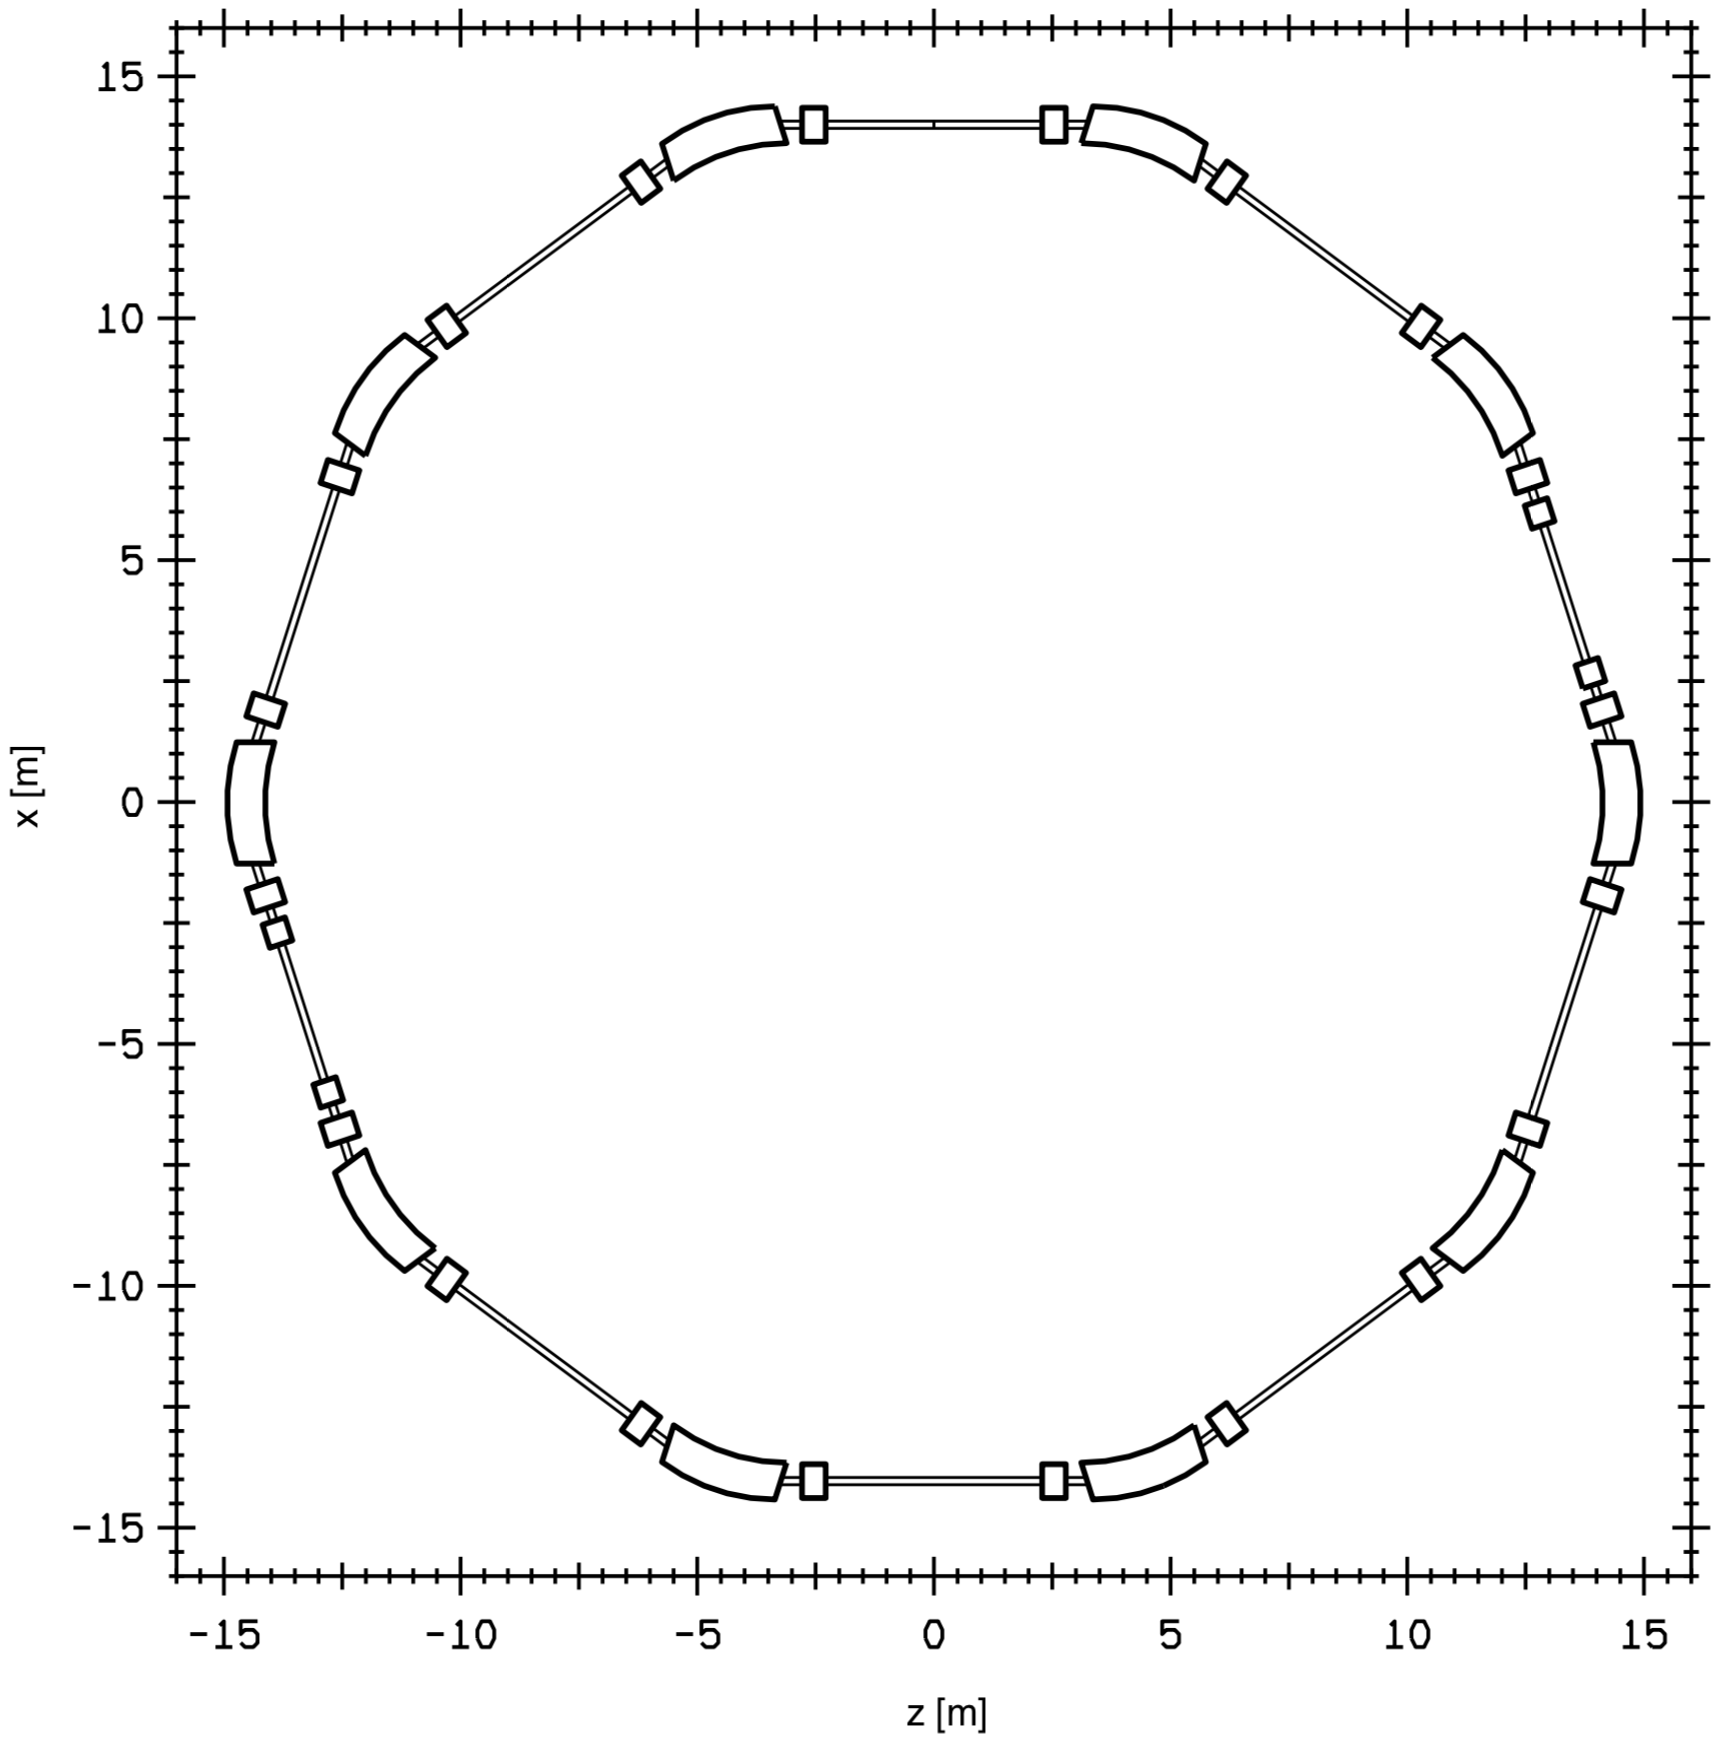
\includegraphics[height=5.75in]{floor}
  \caption{Floor plan of the Proton Storage Ring of section 2.5.  Compare
    with figure 2.5.1.  The $y$ axis is out of the plane of the paper.}
\end{figure}

\newpage
\begin{footnotesize}
\begin{verbatim}
Exhibit 10.13
***MARYLIE 3.0***
Prerelease Development Version 8/21/98
Copyright 1987 Alex J. Dragt
All rights reserved

Data input complete; going into #labor.
#comment
 Exhibit 10.13.
      This is a MaryLie run that employs the geom type code
 to produce a layout drawing using the PSR as an example.
#beam
  4.86914813175970
 0.849425847892200
  1.00000000000000
  1.00000000000000
#menu
 drvs     drft
  0.300000000000000
 drs      drft
  0.450000000000000
 drml     drft
   1.48646000000000
 drl      drft
   2.28646000000000
 bend     pbnd
   36.0000000000000      0.000000000000000E+00  0.500000000000000
   1.20000000000000
 hfq      quad
  0.500000000000000       2.72000000000000      0.000000000000000E+00
  0.000000000000000E+00
 hdq      quad
  0.500000000000000      -1.92000000000000      0.000000000000000E+00
  0.000000000000000E+00
 hcs      sext
  0.500000000000000      0.000000000000000E+00
 vcs      sext
  0.500000000000000      0.000000000000000E+00
 fileout  pmif
   1.00000000000000       12.0000000000000       3.00000000000000
 mapout   ptm
   3.00000000000000       3.00000000000000      0.000000000000000E+00
  0.000000000000000E+00   1.00000000000000
 chrom    tasm
   2.00000000000000      1.000000000000000E-03   1.00000000000000
  0.000000000000000E+00   3.00000000000000      0.000000000000000E+00
 geom     geom
   2.00000000000000      0.000000000000000E+00  0.000000000000000E+00
   1.00000000000000       2.00000000000000      0.000000000000000E+00
 ps1      ps1
   14.0000000000000      0.000000000000000E+00  0.000000000000000E+00
  0.000000000000000E+00  0.000000000000000E+00  0.000000000000000E+00
 ps2      ps2
  0.000000000000000E+00  0.000000000000000E+00  0.000000000000000E+00
   80.0000000000000      0.000000000000000E+00   5.00000000000000
 fin      end
#lines
 nsex
     1*drl         1*hdq         1*drs         1*bend        1*drs      &
     1*hfq         1*drl
 tsex
     1*drl         1*hdq         1*drs         1*bend        1*drs      &
     1*hfq         1*drvs        1*hcs         1*drml
 lsex
     1*drml        1*vcs         1*drvs        1*hdq         1*drs      &
     1*bend        1*drs         1*hfq         1*drl
 half
     1*nsex        1*tsex        1*lsex        1*nsex        1*nsex
 ring
     2*half
 cgeom
     1*ps1         1*ps2         1*geom
#lumps
#loops
 lring
     1*ring
#labor
    1*fileout
    1*lring
    1*cgeom
    1*fin

end of MARYLIE run
\end{verbatim}
\end{footnotesize}


